\documentclass{article}
\usepackage{amsmath,amssymb,amstext,mathtools,array,url,bm,graphicx,color,epsfig}
\usepackage{fullpage,setspace}
\usepackage{authblk}
\usepackage{filecontents}
\usepackage{natbib}
\usepackage{lineno}
\usepackage[colorlinks]{hyperref}
\usepackage{subcaption}
\usepackage{float}
\usepackage[flushleft]{threeparttable}

\def\dt{\partial t}
\def\dx{\partial x}
\def\dy{\partial y}
\def\dz{\partial z}
\def\BE{\begin{equation}}
\def\EE{\end{equation}}
\def\half{\frac{1}{2}}
\def\calT{\cal T}
\def\Deltax{\Delta x}
\def\Deltat{\Delta t}
\DeclareSymbolFont{largesymbolsA}{U}{txexa}{m}{n}
\DeclareMathSymbol{\varprod}{\mathop}{largesymbolsA}{16}


\begin{document}

\title{\bf Modeling of Geophysical Flows -- Analysis of Models and Modeling Assumptions Using UQ}
\author[1]{ Ali A. Safaei}
\author[2]{A. Bevilacqua}
\author[1,3]{Abani K. Patra}
\author[4]{E. B. Pitman}

\affil[1]{\textit{Dept. of Mech. and  Aero. Eng., University at Buffalo, Buffalo NY 14260} }
\affil[2]{\textit{Dept. of Geology., University at Buffalo, Buffalo NY 14260} }
\affil[3]{\textit{Comp. Data Science and Eng., University at Buffalo, Buffalo NY 14260} }
\affil[4]{\textit{Dept. of Materials Design and Innovation, University at Buffalo, NY, 14260}}

\date{\texttt{\{abani,aliakhav,abevilac\}@buffalo.edu}}


\maketitle

\abstract
Dense large scale granular avalanches are a complex class of flows with physics that has often been poorly captured by models that are computationally tractable. Sparsity of actual flow data (usually only a posteriori  deposit information is available) and large uncertainty in the mechanisms of initiation and flow propagation make the modeling task challenging and a
subject of much continuing interest. Models that appear to represent the physics well
 in certain flows turn out to be poorly behaved in others due to intrinsic mathematical or numerical issues.
Nevertheless, given the large implications on life and property many models with different modeling assumptions have been proposed.

While, inverse problems can shed some light on parameter choices it is difficult to make firm judgements on the validity or appropriateness of any single or set of modeling assumptions for a particular target flow or potential flows that needs to be modeled for predictive use in hazard analysis. We will present here an uncertainty quantification  based approach to carefully, analyze the effect of modeling assumptions on quantities of
interest in simulations based on three established models (Mohr-Coulomb, Pouliqen-Fortere and Voellmy-Salm) and thereby derive a model (from a set of modeling assumptions) suitable for use in a particular context. We also illustrate that a simpler though more restrictive approach is to use a Bayesian modeling average approach based on the limited data to combine the outcomes of different models.

\newpage
\section{Geophysical Flows and Review of Models -- Ali}\label{sec:GeoPhFlows}

\subsection{An Overview of Geophysical Flow Types}\label{subsec:FlowTypes}
The term ``geophysical flow'' describes a broad class of flows that covers small mudflows and rockfalls, debris flows, pyroclastic density currents (including pumice and ash and block and ash flows), lava, and dry volcanic debris avalanches. Particles in block and ash flows, debris avalanches, and debris flows typically range from centimeters to meters in size. These flows are sometimes tens of kilometers in length and may travel at speeds as fast as hundreds of meters per second. Their deposits can be as much as 100 meters deep and kilometers long. In other words, there is no single universal description of a ``typical'' geophysical mass flow, even if we restrict ourselves to those flows occurring at a single volcano. Different types of flows are the results of different types of mechanisms/processes and so different types of flows will have significantly different physical characteristics. For the sake of clarification, let us consider three different types of events that are \textit{pyroclastic pumice and ash flow} (resulting from a column collapse), \textit{pyroclastic block and ash flow} (resulting from a dome collapse) an \textit{volcanic debris avalanche}.

A column collapse pyroclastic flow is formed from a vertically-ejected eruption column. Instead of rising in the eruption plume, denser than air material collapses back to the ground and begins to flow as a gravity current. The kinetic energy of the material that lands on the upper slopes of the volcano is therefore redirected into downslope motion. These types of flow involve ash and low density pumiceous material, formed by vesiculation and fragmentation of gas-rich magmas in the volcanic conduit during the explosions. In a column collapse, during the horizontal component of flow, ambient air is entrained into the flow and heated. The flows therefore involve a mixture of hot gas, ash, and small pumice clasts (a few [cm] to 0.5 [m]). This extremely hot mixture can have initial downslope speeds in the range of 30 -- 80 meters per second. The volume of material involved in such a flow is roughly constrained to the volume of the plug and upper conduit (for short-lived explosive eruptions) and therefore will most likely be in the range $10^4$ -- $10^6$ [$\mathrm{m^3}$].

A dome collapse occurs when there is a significant amount of (recently extruded) viscous lava piled up in an unstable configuration around a vent. Further extrusion and/or externals forces such as intense rainfall cause the still hot dome of viscous lava to collapse, disintegrate, and avalanche downhill. The hot, dense blocks in this ``block and ash'' flow will typically range from centimeters to a few meters in size. The matrix is composed of fine ash from the comminuted blocks. The amount of material involved in these collapses is constrained by the size of the newly extruded and still hot dome but usually involves volumes in the range $10^4$ -- $10^8$ [$\mathrm{m^3}$].

A debris avalanche is the failure of a major part of an established volcanic edifice. These usually involve predominantly cold and mechanically weakened rocks as well as large volumes, up to tens of cubic kilometers. The triggering mechanism can be internal (such as the intrusion of new magma and pressurization) or external (such as seismic acceleration, rainfall, etc.). As such, the material involved in these events can be a mixture or fresh magmatic components as well as ancient hydrothermally weakened rocks. The material volume is usually in the range of $10^4$ -- 3$\times10^{10}$ [$\mathrm{m^3}$]. These types of flows are distinguished in that they involve large parts of the edifice that are not thoroughly broken up, i.e. some particles can be up to hundreds of meters or even kilometers in diameter.

\subsection{Modeling Assumptions}\label{subsec:ModelAssump}
As a matter of fact, a very crucial feature of a sophisticated model for geophysical mass flows is that it is based on \textit{physical reasoning} and \textit{rigorous mathematical foundations}. Subsequently, several simplifying, but nevertheless realistic, assumptions were made that streamlined the mathematical formulation. They as follows:
\begin{enumerate}
\item The moving mass was assumed to be \textit{volume preserving}. Since the dynamics define the motion, assuming volume preserving is an adequate approximation.
\item Geophysical mass flows are mostly assumed to be \textit{free surface} flows consist of granular material (i.e. a large collection of discrete particles, frequently with interstitial fluid, and whatever else that get caught in the flow path). In general, the ``typical particle'' is small compared to the depth and length of the flowing mass and makes it reasonable to model the flowing material as a continuum which implies that the thickness of sliding and deforming body extends over several particle diameters. Therefore, we can consider an ``equivalent flowing material'' whose rheological properties are chosen to approximate the bulk behavior that is expected of an actual mass flow; however, the properties of this ``equivalent material'' may not correspond to those of any component of the actual mass flow.
\item According to the \textit{geometries} of geophysical mass flows, numerous models make the \textit{shallowness} approximation for their numerical simulation. In this approximation, the flow depth is assumed to be at least an order of magnitude less than the characteristic length of the flowing material.
\item The shear stresses lateral to the main flow direction can be neglected.
\item The body of mass is supposed to be in \textit{isothermal} state or, if not, thermal effects can be ignored.
\item The flowing mass is assumed to be consisted of an \textit{incompressible} granular continuum material. This means that we are allowed to ignore variations of density due to the void ratio (density preserving assumption).
\item Motion of the bulk of mass consists of ``shearing within the deforming mass'' and ``sliding along the basal surface''. However, based on the observations, the shearing deformation commonly takes place within a very small boundary layer, so that it is justified to collapse this boundary layer to zero thickness and to combine the sliding and shearing velocity to a single sliding law with a somewhat larger modelled \textit{sliding velocity}. This then effectively means that variations of the material velocities across the flow depth may be ignored and \textit{depth-averaged} equations may be employed \citep{SavageHutter,Hutter1993}. Details on the integration of continuum models for shallow free surface flows can be studied in \citep{PudasainiHutter2007}.%This method was introduced by Von K\'{a}rm\'{a}n and later refined by Pohlhausen, where the equations are averaged over depth and the velocity profile is assumed.
\item The shallowness assumption gives a \textit{hydrostatic} expression for the normal pressure in the direction perpendicular to the basal surface. Moreover, the downslope and cross-slope pressure components are assumed to be varying linearly with the normal pressure component through the flow depth. The coefficient could either be defined based on the rheology model or be constant \citep{SavageHutter,Bartelt1999,Iverson2001,Denlinger2001}.
\end{enumerate}
%This list is not comprehensive across the many models that have been proposed for such flows.
\subsection{Governing Equations and Boundary Conditions}\label{subsec:GovEqsBCs}
Starting with the basic conservation of mass and momentum for an incompressible medium, we can describe the motion of an avalanching mass:
\begin{eqnarray}\label{eq:N_S}
\nabla \cdot\underline{{\textbf u}} &=& 0, \nonumber \\
\dfrac{\partial}{\dt}(\rho \ \underline{{\textbf u}})+\nabla \cdot (\rho \ \underline{{\textbf u}}\otimes \underline{{\textbf u}}) &=& \nabla \cdot \underline{\underline{{\mathbf{T}}}}+\rho \ \underline{{\textbf g}},
\end{eqnarray}
Where $\underline{{\textbf u}}=[u, v, w]^{\mathrm{T}}$, is the material velocity vector, $\rho$ is its constant density, $\underline{\underline{{\mathbf{T}}}}$ is the \textit{Cauchy} stress tensor, and $\underline{{\textbf g}}$ is the gravity vector. Based on the material rheology we choose, the Cauchy stress tensor, $\underline{\underline{{\mathbf{T}}}}$, is defined differently \citep{FreundtBursik1998}. Defining the free and basal surface interfaces respectively as follows,
\begin{eqnarray}\label{eq:surfacesDefs}
F^s(x,y,t) &=& s(x,y,t)-z, \nonumber \\
F^b(x,y,t) &=& b(x,y,t)-z,
\end{eqnarray}
Therefore, one can impose the \textit{kinematic boundary conditions} at free and basal surface interfaces:
\begin{equation}\label{eq:SurKinBC}
\frac{\partial F^s}{\dt} + \underline{{\textbf u}}\cdot\nabla F^s = 0, \ \ at \ F^s(x,y,t)=0
\end{equation}
\begin{equation}\label{eq:BedKinBC}
\frac{\partial F^b}{\dt} + \underline{{\textbf u}}\cdot\nabla F^b = 0, \ \ at \ F^b(x,y,t)=0
\end{equation}
According to the $\mathrm{2^{nd}}$ and $\mathrm{7^{th}}$ assumptions, we may also impose the traction-free boundary condition at the free surface, while a \textit{Coulomb dry-friction} sliding law at the interface between the granular flow and the basal surface is imposed:
\begin{equation}\label{eq:SurTracBC}
\underline{\underline{{\mathbf{T}}}}^s\underline{n}^s=\underline{0}, \ \ at \ F^s(x,y,t)=0
\end{equation}
\begin{equation}\label{eq:BedTracBC}
\underline{\underline{{\mathbf{T}}}}^b\underline{n}^b-\underline{n}^b(\underline{n}^b\cdot \underline{\underline{{\mathbf{T}}}}^b\underline{n}^b)=\frac{\underline{{\textbf u}}^b}{\Vert\underline{{\textbf u}}^b\Vert}(\underline{n}^b\cdot \underline{\underline{{\mathbf{T}}}}^b\underline{n}^b)\mu_{\mathrm{Bed}}, \ \ at \ F^b(x,y,t)=0
\end{equation}
where $\mu_{\mathrm{Bed}}$ is the basal friction coefficient and the basal and surface unit normals are:
\begin{equation}
\underline{n}^b=\frac{\nabla F^b}{\Vert\nabla F^b\Vert}, \ \ \underline{n}^s=\frac{\nabla F^s}{\Vert\nabla F^s\Vert}.
\end{equation}
It is worth mentioning that $\underline{\underline{{\mathbf{T}}}} \ \underline{n}$ is a resisting traction, while $\underline{n}\cdot\underline{\underline{{\mathbf{T}}}} \ \underline{n}$ is the normal pressure and $\underline{n}\cdot\underline{\underline{{\mathbf{T}}}}-\underline{n}(\underline{n}\cdot\underline{\underline{{\mathbf{T}}}} \ \underline{n})$ is the resusting shear traction. Considering Equation (\ref{eq:BedTracBC}), Coulomb dry-friction sliding law expresses that the magnitude of the basal shear stress is equal to the normal basal pressure multiplied by the basal friction coefficient, $\mu_{\mathrm{Bed}}$. Furthermore, Equation (\ref{eq:BedTracBC}) is stating that the shear traction is assumed to point in the opposite direction to the basal velocity, $\underline{{\textbf u}}^b$ (resisting shear traction) which also implicitly assumes that $\underline{{\textbf u}}^b\cdot \underline{n}^b=0$ when we also consider the basal kinematic boundary condition.

\subsection{Models}\label{subsec:Models}

\section{UQ Process}
The key purpose of this study is to present a procedure for the improved exploration and quantitative comparison of physical models and their assumptions through the collection of full statistical data. Models are not black boxes, behind each physical model there are different physical assumptions, and therefore it would be more appropriate to look at those instead than at the entire model results. Our statistical approach enables a first step towards a data driven selection of the best modeling assumptions to use.

In particular, a good forecasting capability in the context of mass flows requires the careful selection of the pair $(M(A), P(M(A)))$, where $A$ is a set of assumptions, $M(A)$ is the model which combines those assumptions, and $P(M)$ is a probability distribution in the parameter space of $M$. An assumption is a quite general concept - for example it can be a specific equation for the internal stress, the implementation of bed curvature effects, of active-passive material stretching, or the use of a specific correction on the pressure effects, etc... Assumptions are what makes the models being different, and each model may be seen as the combined result of a set of assumptions. Sometimes a good model contains a useless assumption that may be removed, sometimes a good assumption should be implemented inside a different model - those are usually considered as subjective choices, not data driven. Moreover, the correct assumptions may change through time, making the analysis more difficult.

It is worth mentioning that whereas the support of $P(M)$ can be restricted to a single point in case an optimization procedure is performed for the reconstruction of a particular flow, this is not possible if we are interested in the general predictive capabilities of the model, i.e. what is desired in probabilistic hazard assessment. In this study we will always assume $P(M)\sim \varprod_{i=1}^{N_M} Unif(a_{i,M},b_{i,M})$, where $N_M$ is the number of parameters of $M$. These parameter ranges will not be selected under the influence of a particular observation, but we will try to use the information gathered in literature about the physical meaning of those values.

In general, the simulation algorithms can be classified as:
$$\textmd{(1)INPUT VARIABLES} \longrightarrow \textmd{(2)DYNAMICAL QUANTITIES} \longrightarrow \textmd{(3)OBSERVABLE OUTPUTS}$$

The input variables can include: volume, rheology coefficients, initiation site and geometry, digital elevation map. We will focus on the former two of those, the volume of the pile and the rheology, which constitute our parameter space in all the case studies. The dynamical quantities are directly related to the force terms in the Newton Equations that rule the simulation, they include: driving and dissipative stresses and powers. The terms of the equations are hidden to the observation, but they directly depend on the parameters, and represent a fundamental link between the parameters and the observable outputs. Moreover, the models share some of those terms while change others, and this enables a detailed comparison of the real physics below the curtain. Finally, the observable outputs include: flow height, inundated area, flow velocity and acceleration. In the sequel (2) and (3) are also called quantities of interest (QoI).

Another level of complexity can be achieved choosing the degree of integration of (2) and (3) in the previous scheme:
\begin{description}
  \item[(A)] LOCAL MEASUREMENTS
  \item[(B)] SPATIAL AVERAGES
  \item[(C)] TEMPORAL AVERAGES
  \item[(D)] SPATIO-TEMPORAL (FULL) AVERAGES
\end{description}

In particular, all the dynamical quantities, and most of the observable outputs, have a local meaning. They are calculated on the elements of the numerical mesh created by the code. Moreover, all those quantities are time dependent. Differences in time and location enable to constrain the changes in flow regime. Those are really important because if the flow behavior is radically different, then the significance and effects of the assumptions may also change.

A first approach to look at the data is to choose a reasonable design of spatial locations and to calculate the graph of the quantities as a function of time. A second approach is to make the spatial integral of those quantities and calculate their temporal graph - this integration can be done with respect to the basal area, e.g. for the stresses and related powers, or with respect to the flow volume, e.g. velocity and acceleration. A third possible approach requires to make the integrals through time at each designed spatial site, a fourth approach the full integral in space-time.

In general, for each QoI and degree of integration, during a Monte Carlo simulation we sample the input variables and obtain a family of temporal graphs in (A), (B), and numeric values in (C), (D). These results are statistically summarized - plotting their expectation, their standard deviation, their 5th and 95 percentiles. Their correlation structure is also explored, presenting the plots of the Pearson coefficients of the most interesting pairs of quantities in (1), (2), (3). In the following, we will detail the considered input variables and quantities of interest for each of our cases study.

Our sampling technique of the input variables is based on the Latin Hypercube idea, and in particular, on the orthogonal array-based Latin Hypercubes (Tang 1993).

\subsection{Latin Hypercubes and orthogonal arrays}
The Latin Hypercube Sampling (LHS) is a well established procedure for defining pseudo-random design of samples in $\mathbb R^d$ which have: (i) enhanced capability to fill the d-dimensional space, (ii) avoid overlapping of point locations in the one dimensional projections, (iii) reduce the dependence of the number of points necessary on the dimensionality $d$.

The procedure is simple: once the desired number of samples $N\in\mathbb N$ is selected, then the d-dimensional projections are divided in $N$ equal bins, and each bin will contain one and only one sample. There are a large number of possible designs, corresponding the number of permutations of the bins in the d-projections, i.e. $d\cdot N!$. If the permutations are randomly sampled there is a high possibility that the design will have good properties. However, this is not assured.

For this reason, we base our design on the orthogonal arrays (OA). An orthogonal array is an $n\times m$ matrix $Q$ with entries from a set of $s\ge 2 $ symbols. $Q$ is called an $OA(n,m,s,r)$ of strength $r$, size $n$, with $m$ constrains, and $s$ levels if each $n\times r$ submatrix of $Q$ contains all possible $1\times r$ row vectors with the same frequency $\lambda=n/s^r$, which is called the index of the array. Orthogonal arrays are very useful for defining latin hypercubes which are constrained to fill the space (or its r-dimensional subspaces) in a sufficient way.

Let $Q$ be an $OA(n,m,s,r)$. Then for each column of $Q$ we replace the $\lambda s^{r-1}$ elements with entry $k$ by a random permutation of $\left((k-1)\lambda s^{r-1} + h\right)_{h\in 1,\dots, \lambda s^{r-1}}$. After the replacement procedure is done, the newly obtained matrix $U$ is a LHS which inherits from $Q$ the property of fully covering $s^r$ equal r-dimensional hypercubes in every r-dimensional projection. Each hypercube contains $\lambda$ points. In other words, inside each r-dimensional projection, the design associated to $U$ fills the space like a regular grid at the scale of those $s^r$ hypercubes, but it is still an LHS at a finer scale, i.e. the $\lambda s^{r-1}$ one dimensional bins.

What happens in the projections with dimension $r'>r$ is not controlled, and randomizing procedures are made more difficult by the additional structure imposed by the $OA$. Moreover, the total number of points necessary to achieve a full design increases with $r$, and hence is affected by dimensionality issues.

Dealing with relatively small $d$, i.e. $d\in\{3,4\}$, we adopt a LHS $U$ created by a $OA(s^d,d,s,d)$. The strength is equal to the dimension $d$, hence the design fills the entire space like a $d$ dimensional grid, but it is a LHS as well. In this case there is one point in each hypercube, and $\lambda=1$. We took $s=8$ for the 3-dimensional designs, i.e. $512$ points; we took $s=6$ for the 4-dimensional designs, i.e. 1296 points.

\section{QoIs and Data Collected}
\subsection{Flow down an inclined plane}
In order to investigate the effects of constituent elements of each rheology model, we are interested in computing the quantitative contribution of each force component (gravitational, basal friction and material resistence forces) to the time evolution of the flowing material. However, there is not a straight forward way to simply obtain the quantitative contribution of these force components. The reason is that ``total force'' is not necerssarily a positive/negative or non-zero figure along time that we can simply extract the contribution of each force component based on it; therefore, the leading force component may vary with time. Furthermore, we there is no precise way to carry out this study without considering the spatial effects for the bulk of flowing material just as function of time. As a result, we pick four different locations on the planes center line, $y=0$, that are the slumping pile location ($x=-0.7$), middle of the inclined plane ($x=-0.35$), joint location of inclined and runout planes ($x=0.0$), and on the runout plane ($x=0.15$). According to the specified threshold for flow thickness, $h>1.0$ mm, we may consider temporal invaded region and check if the specified locations are inside that region. If so, we may find the maximum absolute value of force elements along each direction so that we can obtain the magnitude and type of ``dominant'' force elements, $\vert F_{\mathrm{dominant}}\vert$, along runout and lateral directions. Having computed temporal $\vert F_{\mathrm{dominant}}(t)\vert$, we now divide all the force components by $\vert F_{\mathrm{dominant}}(t)\vert$, so that the resulting quotients, $q_i(t)_{i=1,2,3,4}$, show us the temporal impact of each force type and its direction at the specified locations. We should consider that if $q_{\mathrm{dominant}}(t)=\pm 1$, the $i^\mathrm{{th}}$ force component is the dominant one and the other three non-dominant quotients would be $0 \leq \vert q_i(t) \vert < 1$. This is true for a sample simulated flow; however, when we consider the entire flow regime inside an ensemble of simulations, we can take the mean values of $q_i(t)$ as fair measure for the temporal impact of each force type and its direction (with respect to the flow direction) along the whole ensemble range. We should note that after taking the mean values of $\bar{q}_i(t)$, the dominant ones are \textit{not necessarily} $\bar{q}_{\mathrm{dominant}}(t)=\pm 1$; nevertheless, their absolute values are larger than other non-dominant averaged quotients. the following three sections include the results of the impact quotients, $\bar{q}_i(t)$ for the three rheology models of our study.
\subsubsection{Mohr-Coulomb Model, Force Impact Quotients}
\begin{figure}[H]
        \begin{minipage}[b]{0.5\linewidth}
                \centering
                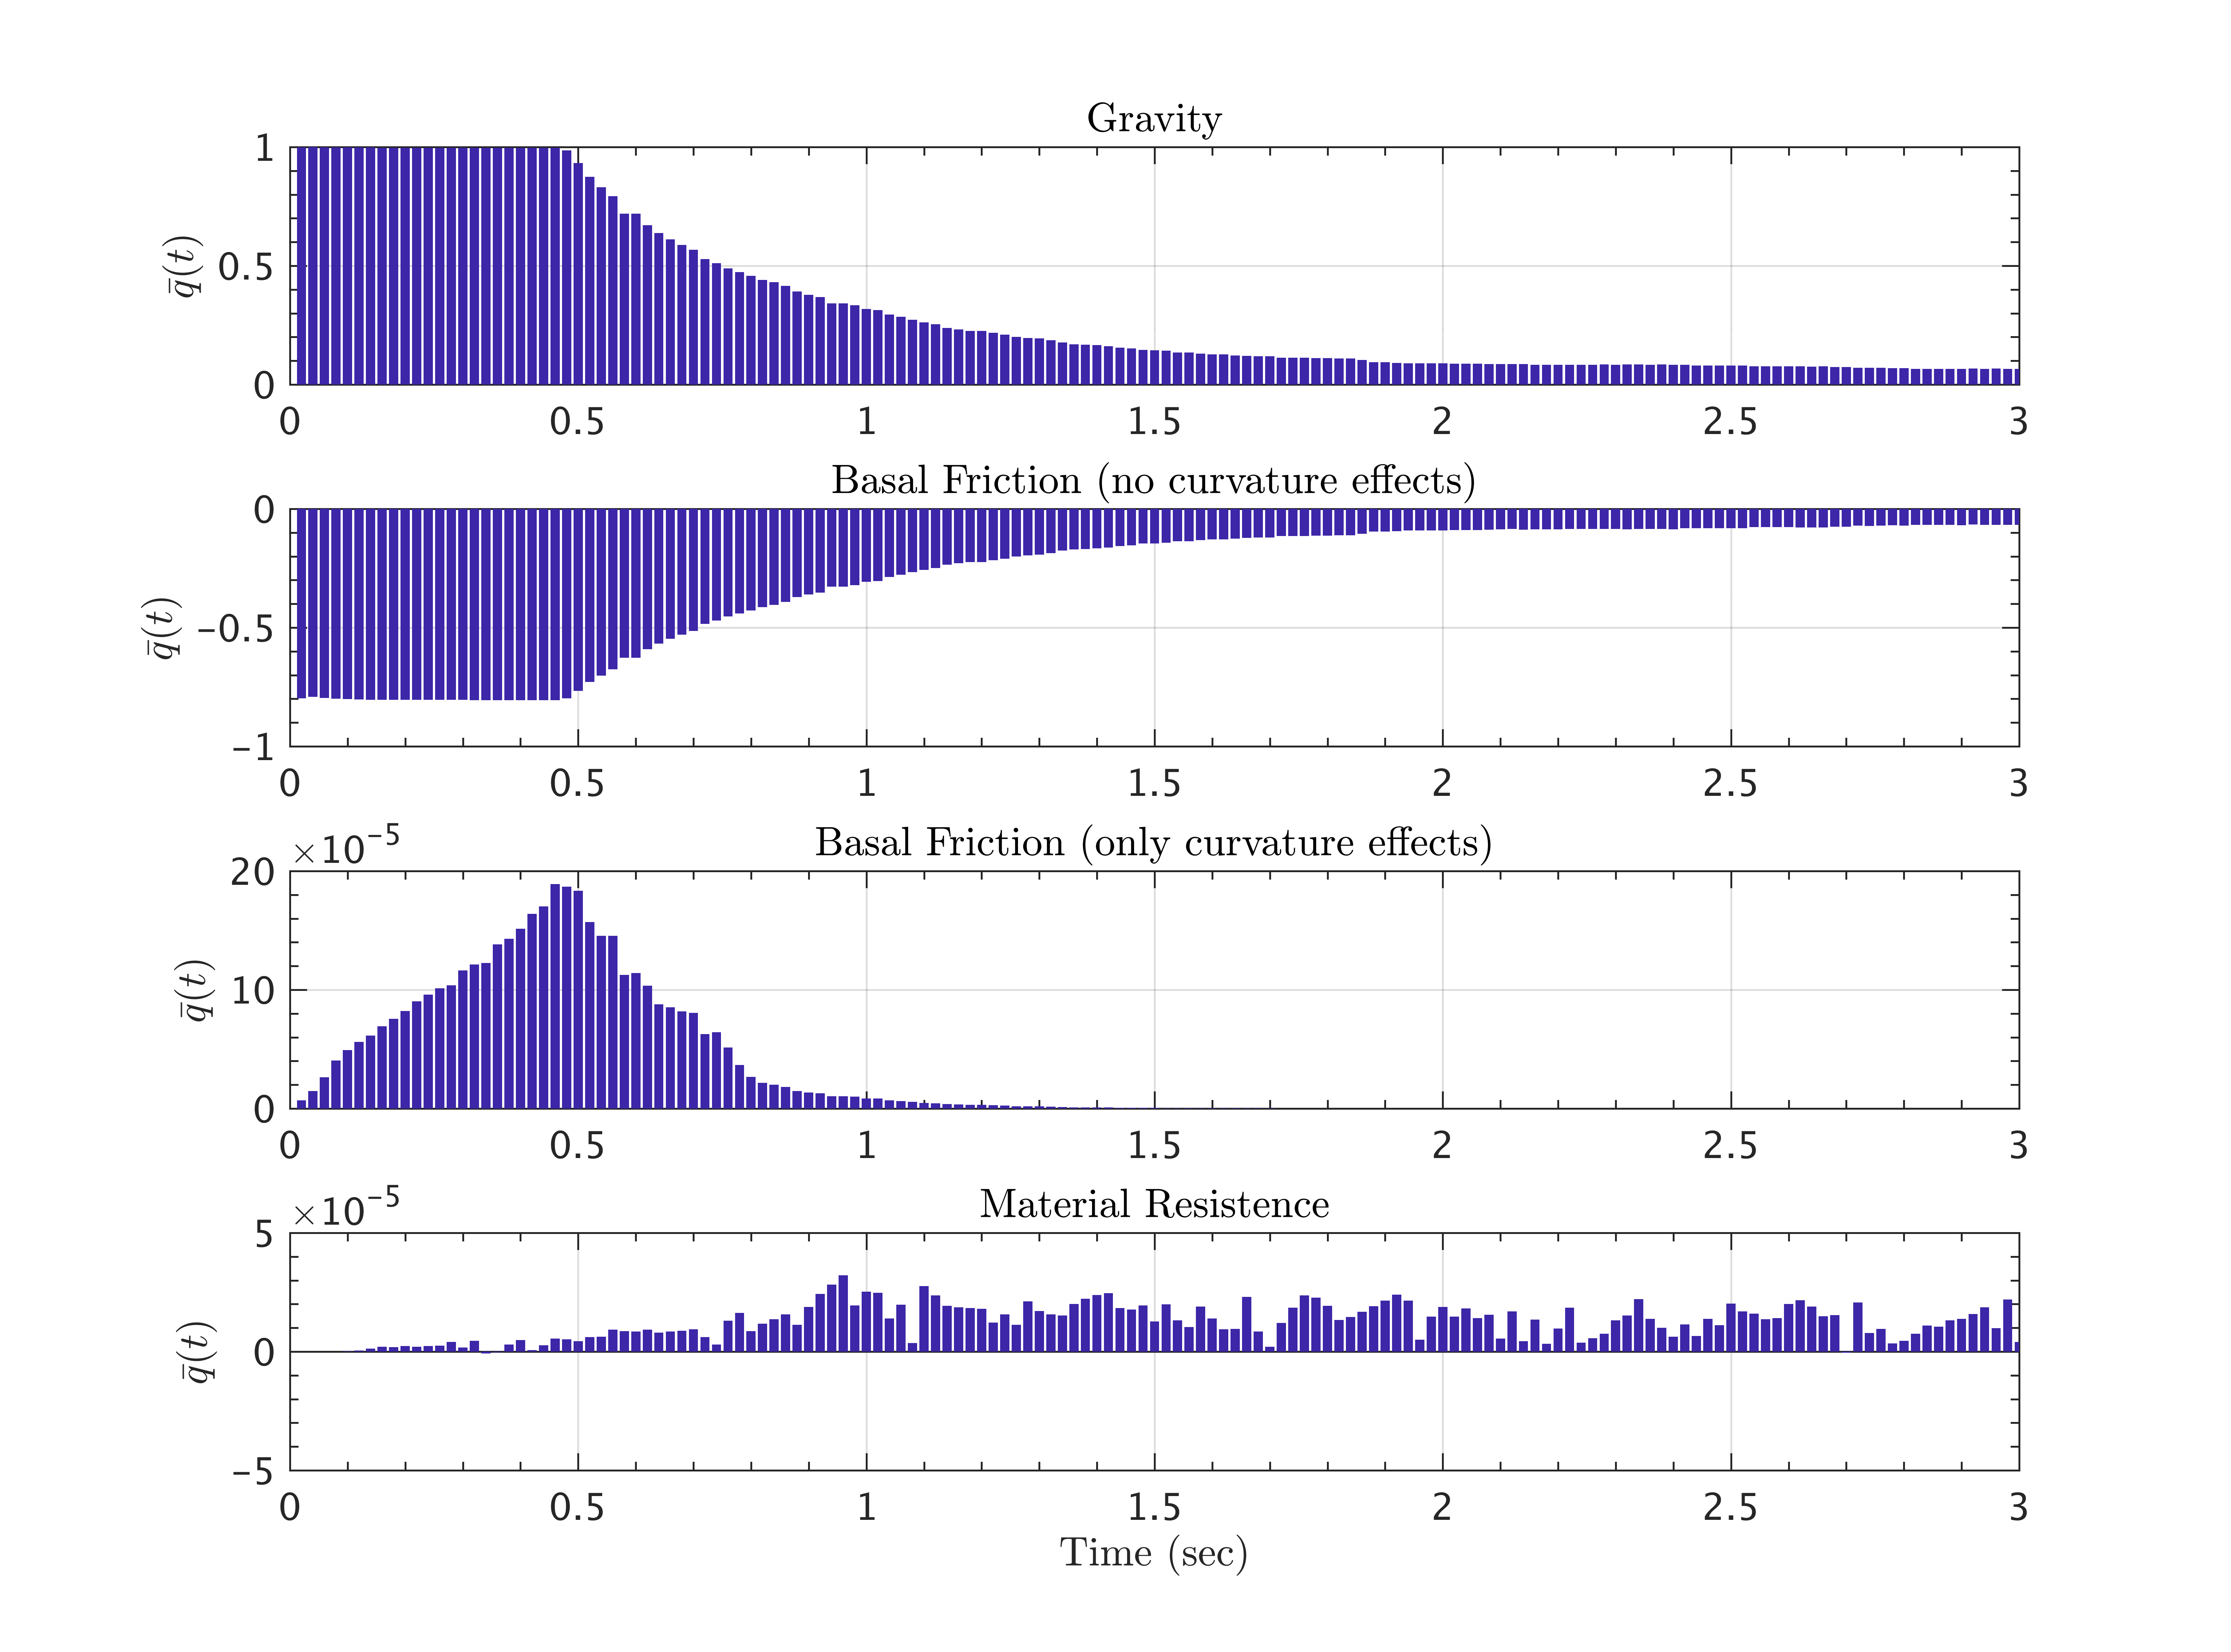
\includegraphics[width=1\textwidth]{InclinedPlane/LocalRecords/ContribF1_C_x.png}
                \subcaption{$x=-0.7, \ y=0.0$, slumping pile location.}
                \label{fig:Ramp-Cx1}
        \end{minipage}
        \begin{minipage}[b]{0.5\linewidth}
                \centering
                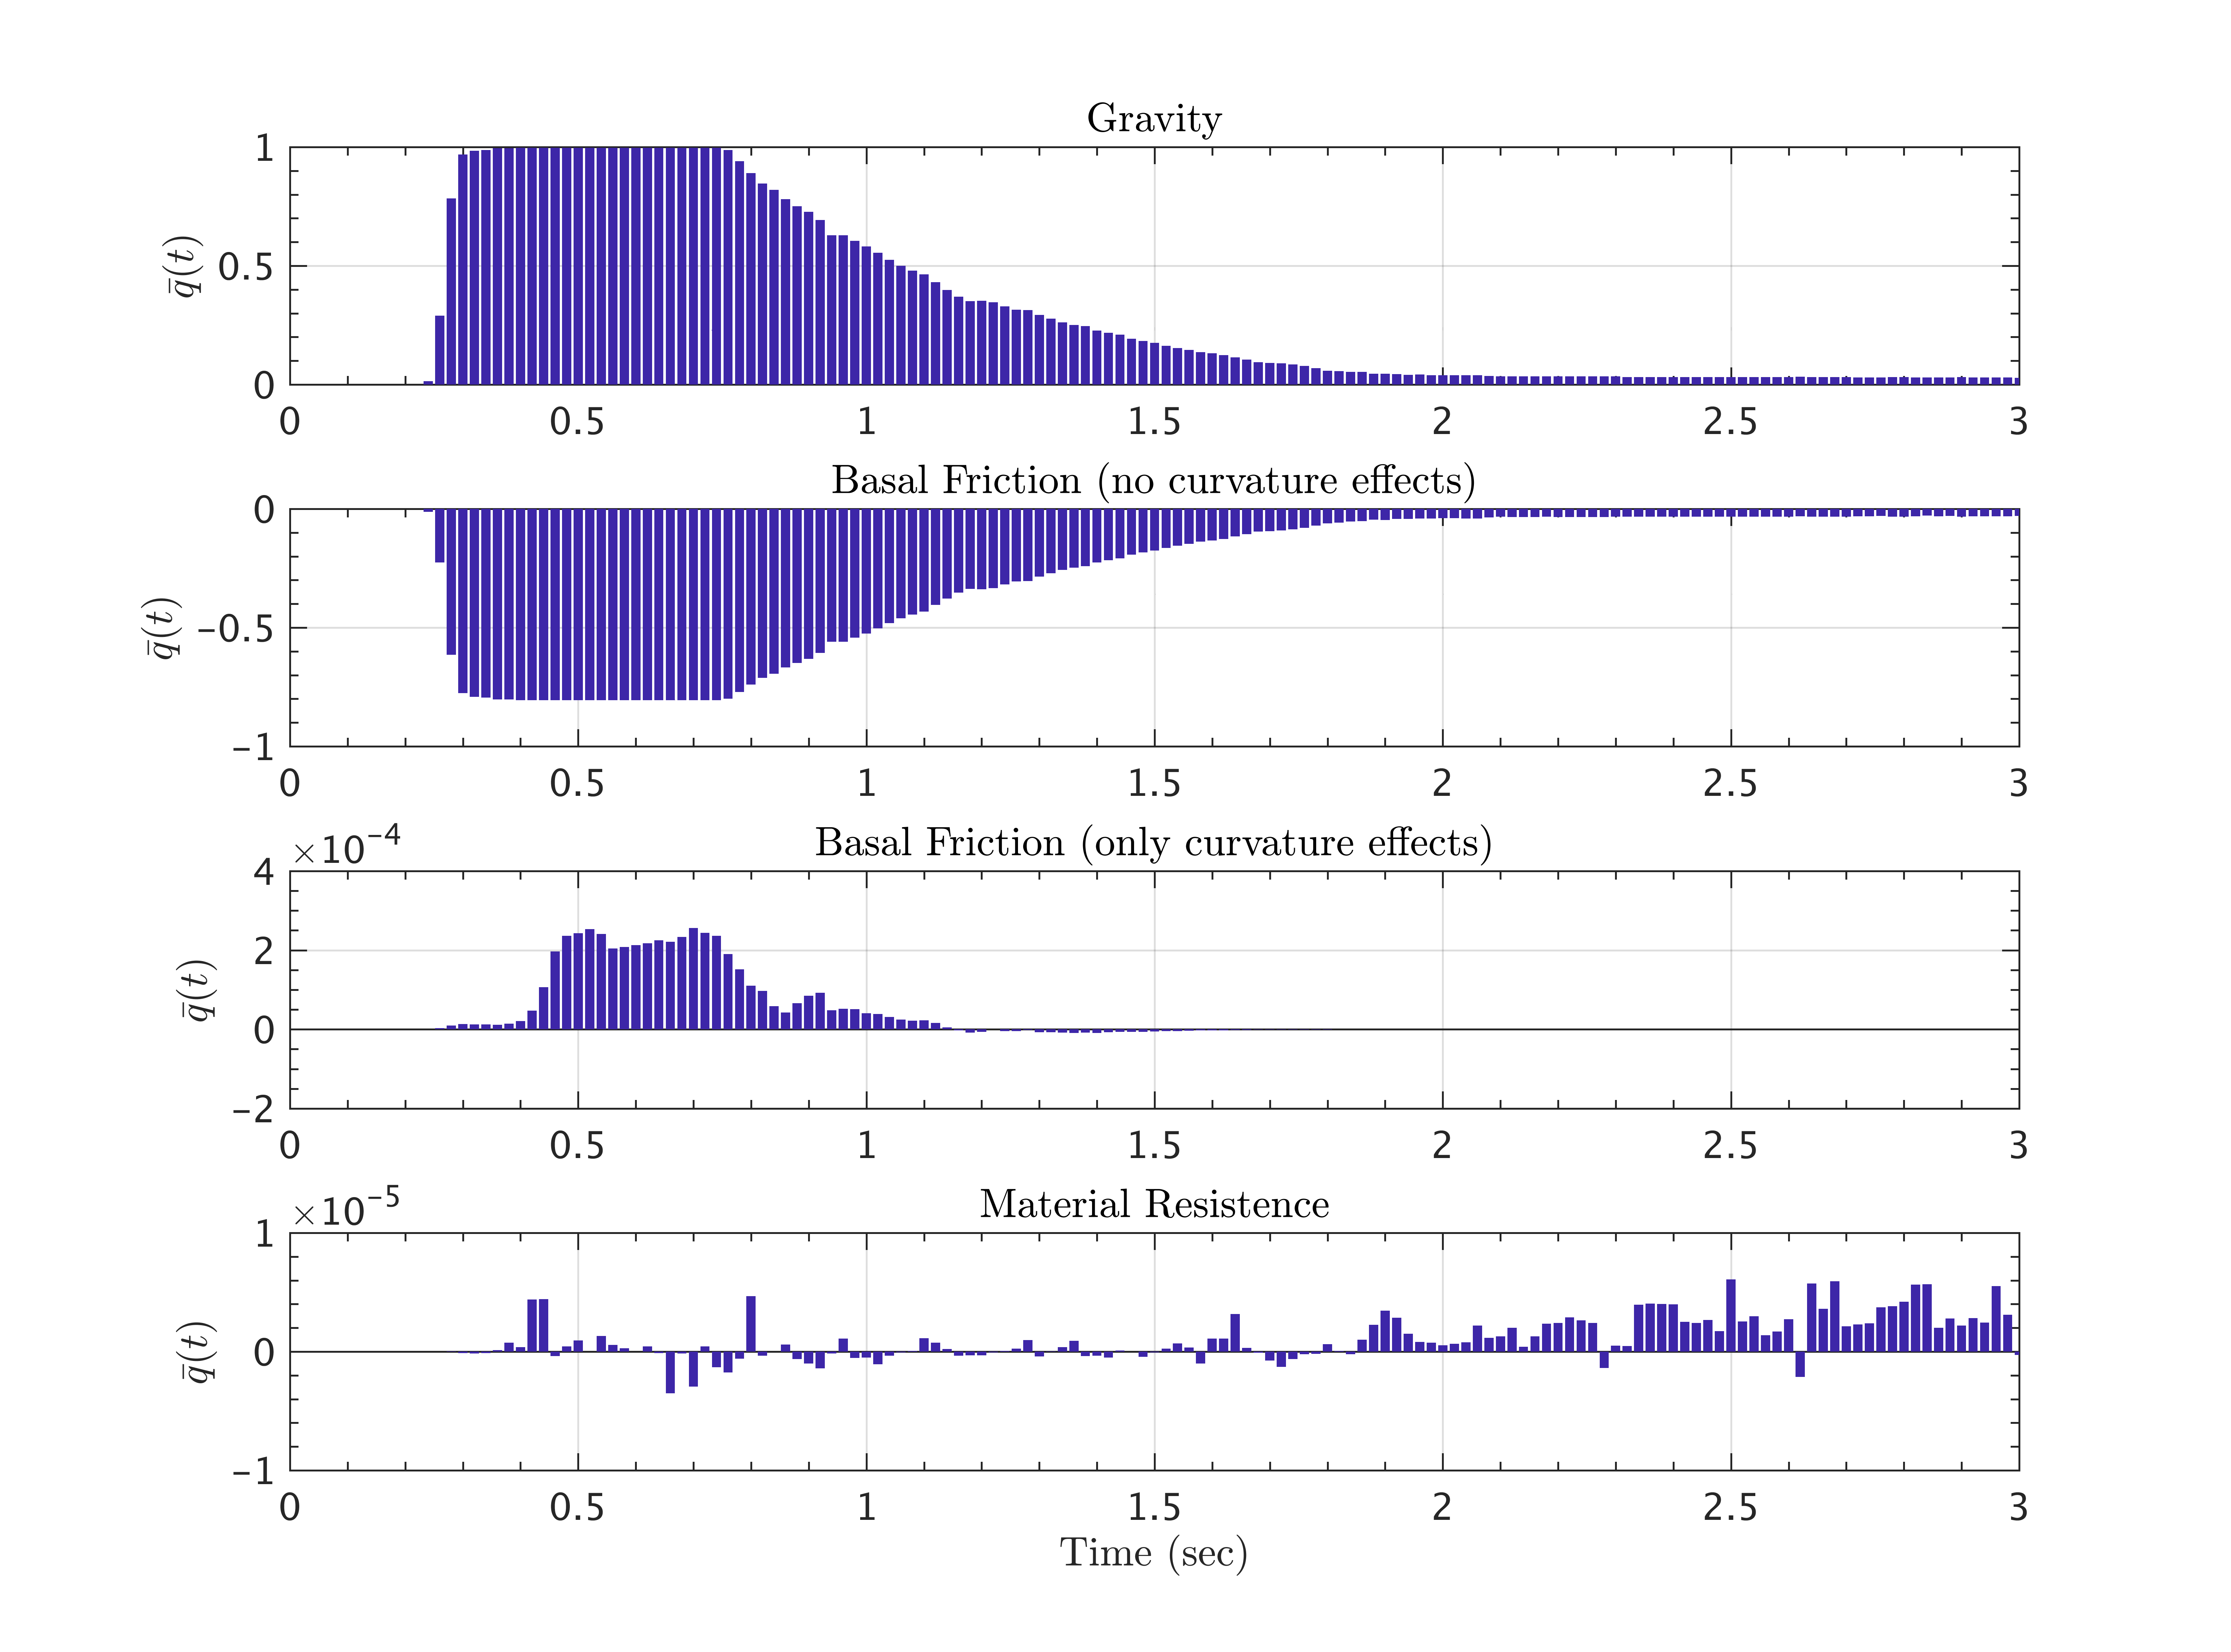
\includegraphics[width=1\textwidth]{InclinedPlane/LocalRecords/ContribF8_C_x.png}
                \subcaption{$x=-0.35, \ y=0.0$, middle point on inclined plane.}
                \label{fig:Ramp-Cx2}
        \end{minipage}

        \begin{minipage}[b]{0.5\linewidth}
                \centering
                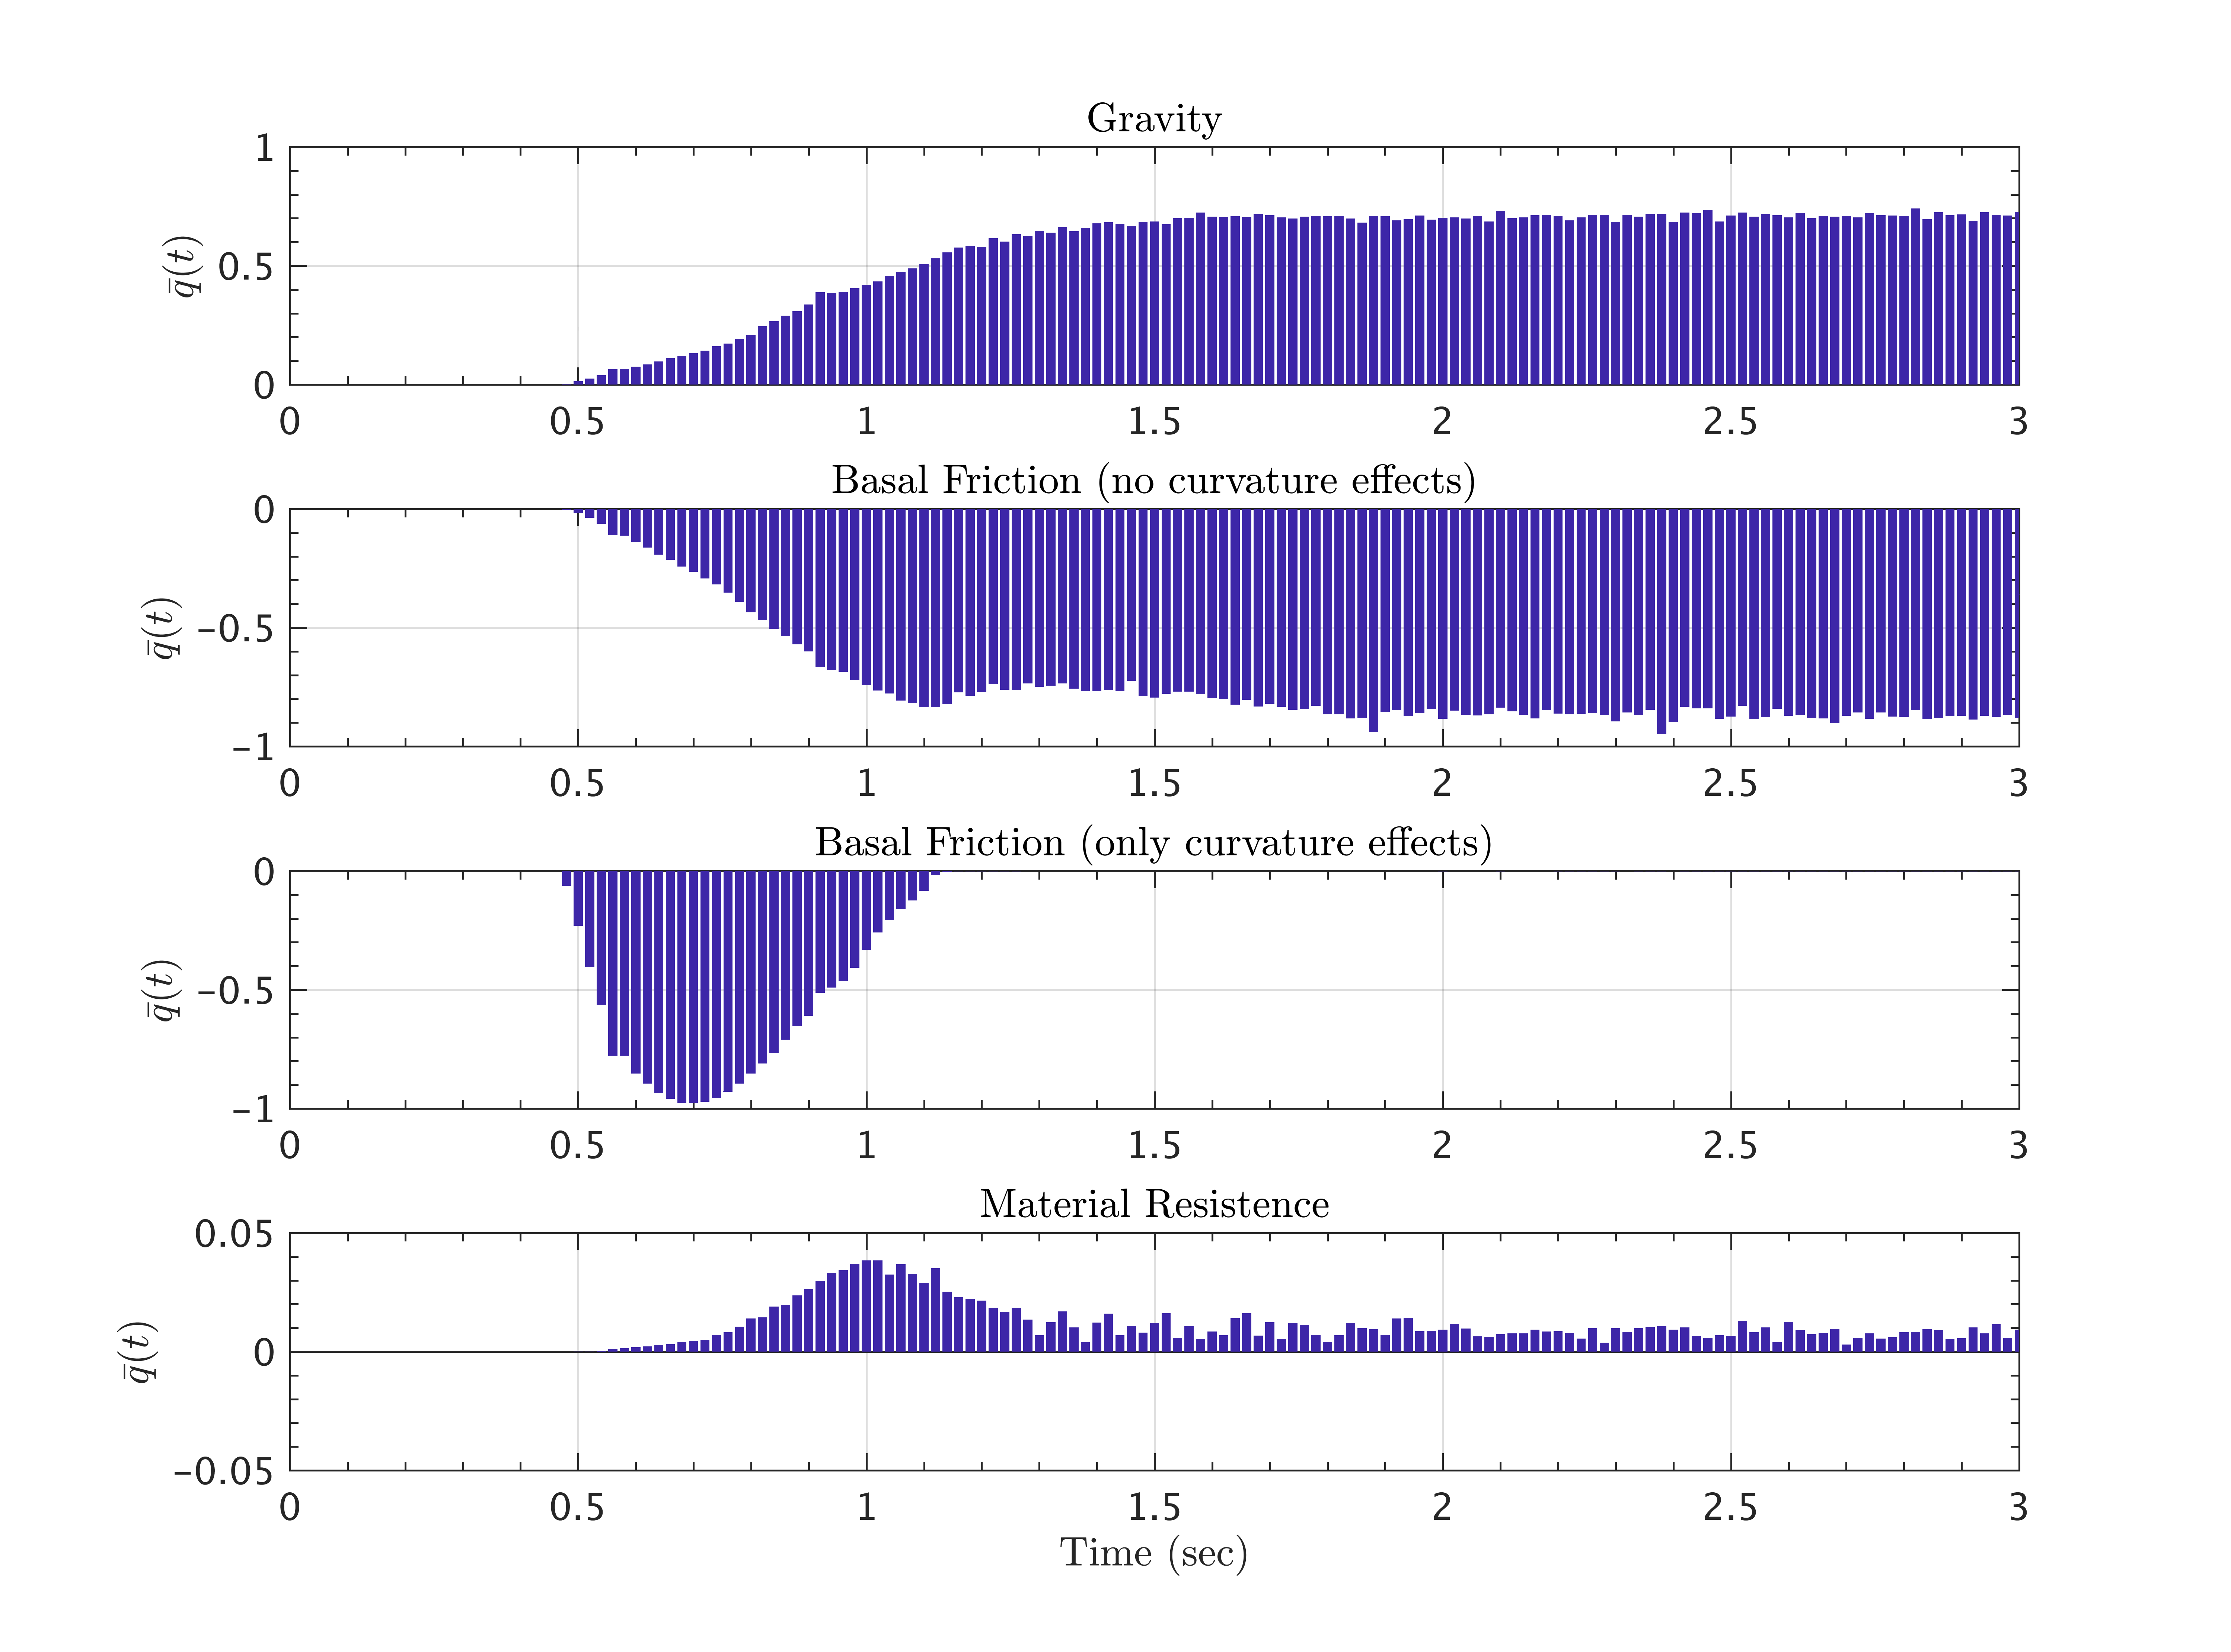
\includegraphics[width=1\textwidth]{InclinedPlane/LocalRecords/ContribF15_C_x.png}
                \subcaption{$x=0, \ y=0$, inclined and runout planes' joint location.}
                \label{fig:Ramp-Cx3}
        \end{minipage}
        \begin{minipage}[b]{0.5\linewidth}
                \centering
                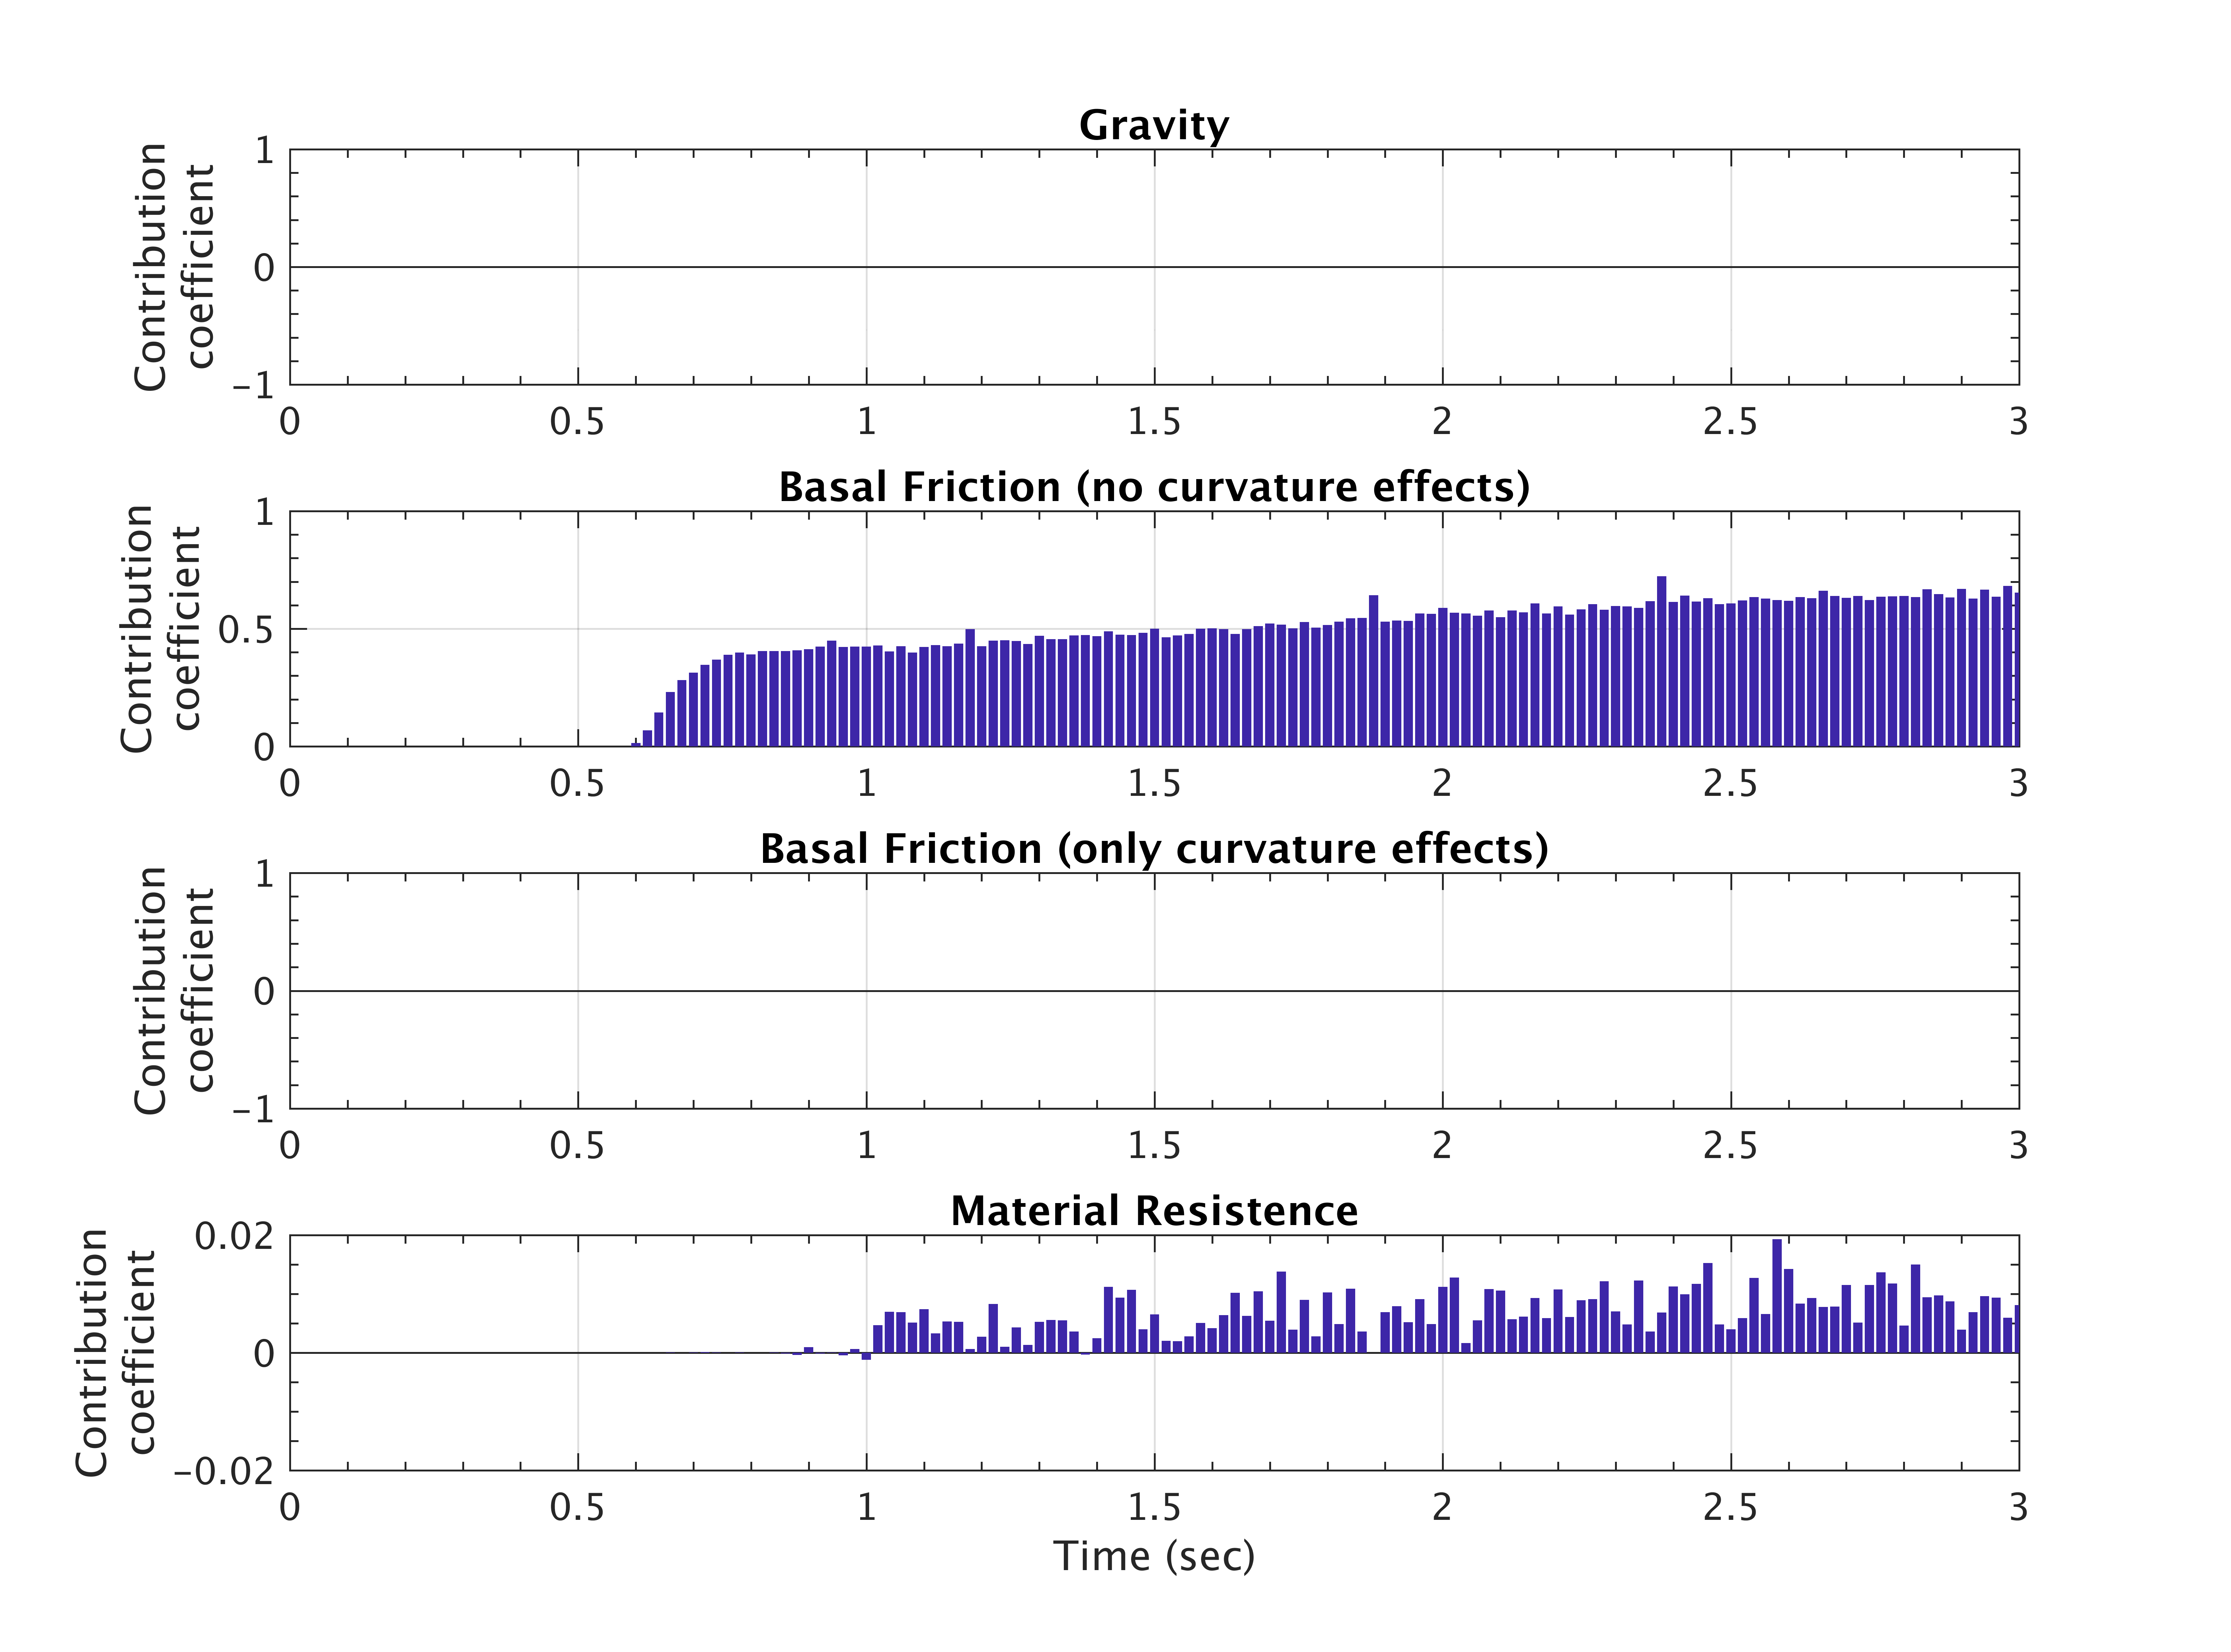
\includegraphics[width=1\textwidth]{InclinedPlane/LocalRecords/ContribF17_C_x.png}
                \subcaption{$x=0.15, \ y=0.0$, a location on runout plane.}
                \label{fig:Ramp-Cx4}
        \end{minipage}
        \caption{Time history of mean values for force impact quotients, $\bar{q}_i(t)$, along runout direction, Mohr-Coulomb model.}
        \label{fig:Ramp-Cx}
\end{figure}

\begin{figure}[H]
        \begin{minipage}[b]{0.5\linewidth}
                \centering
                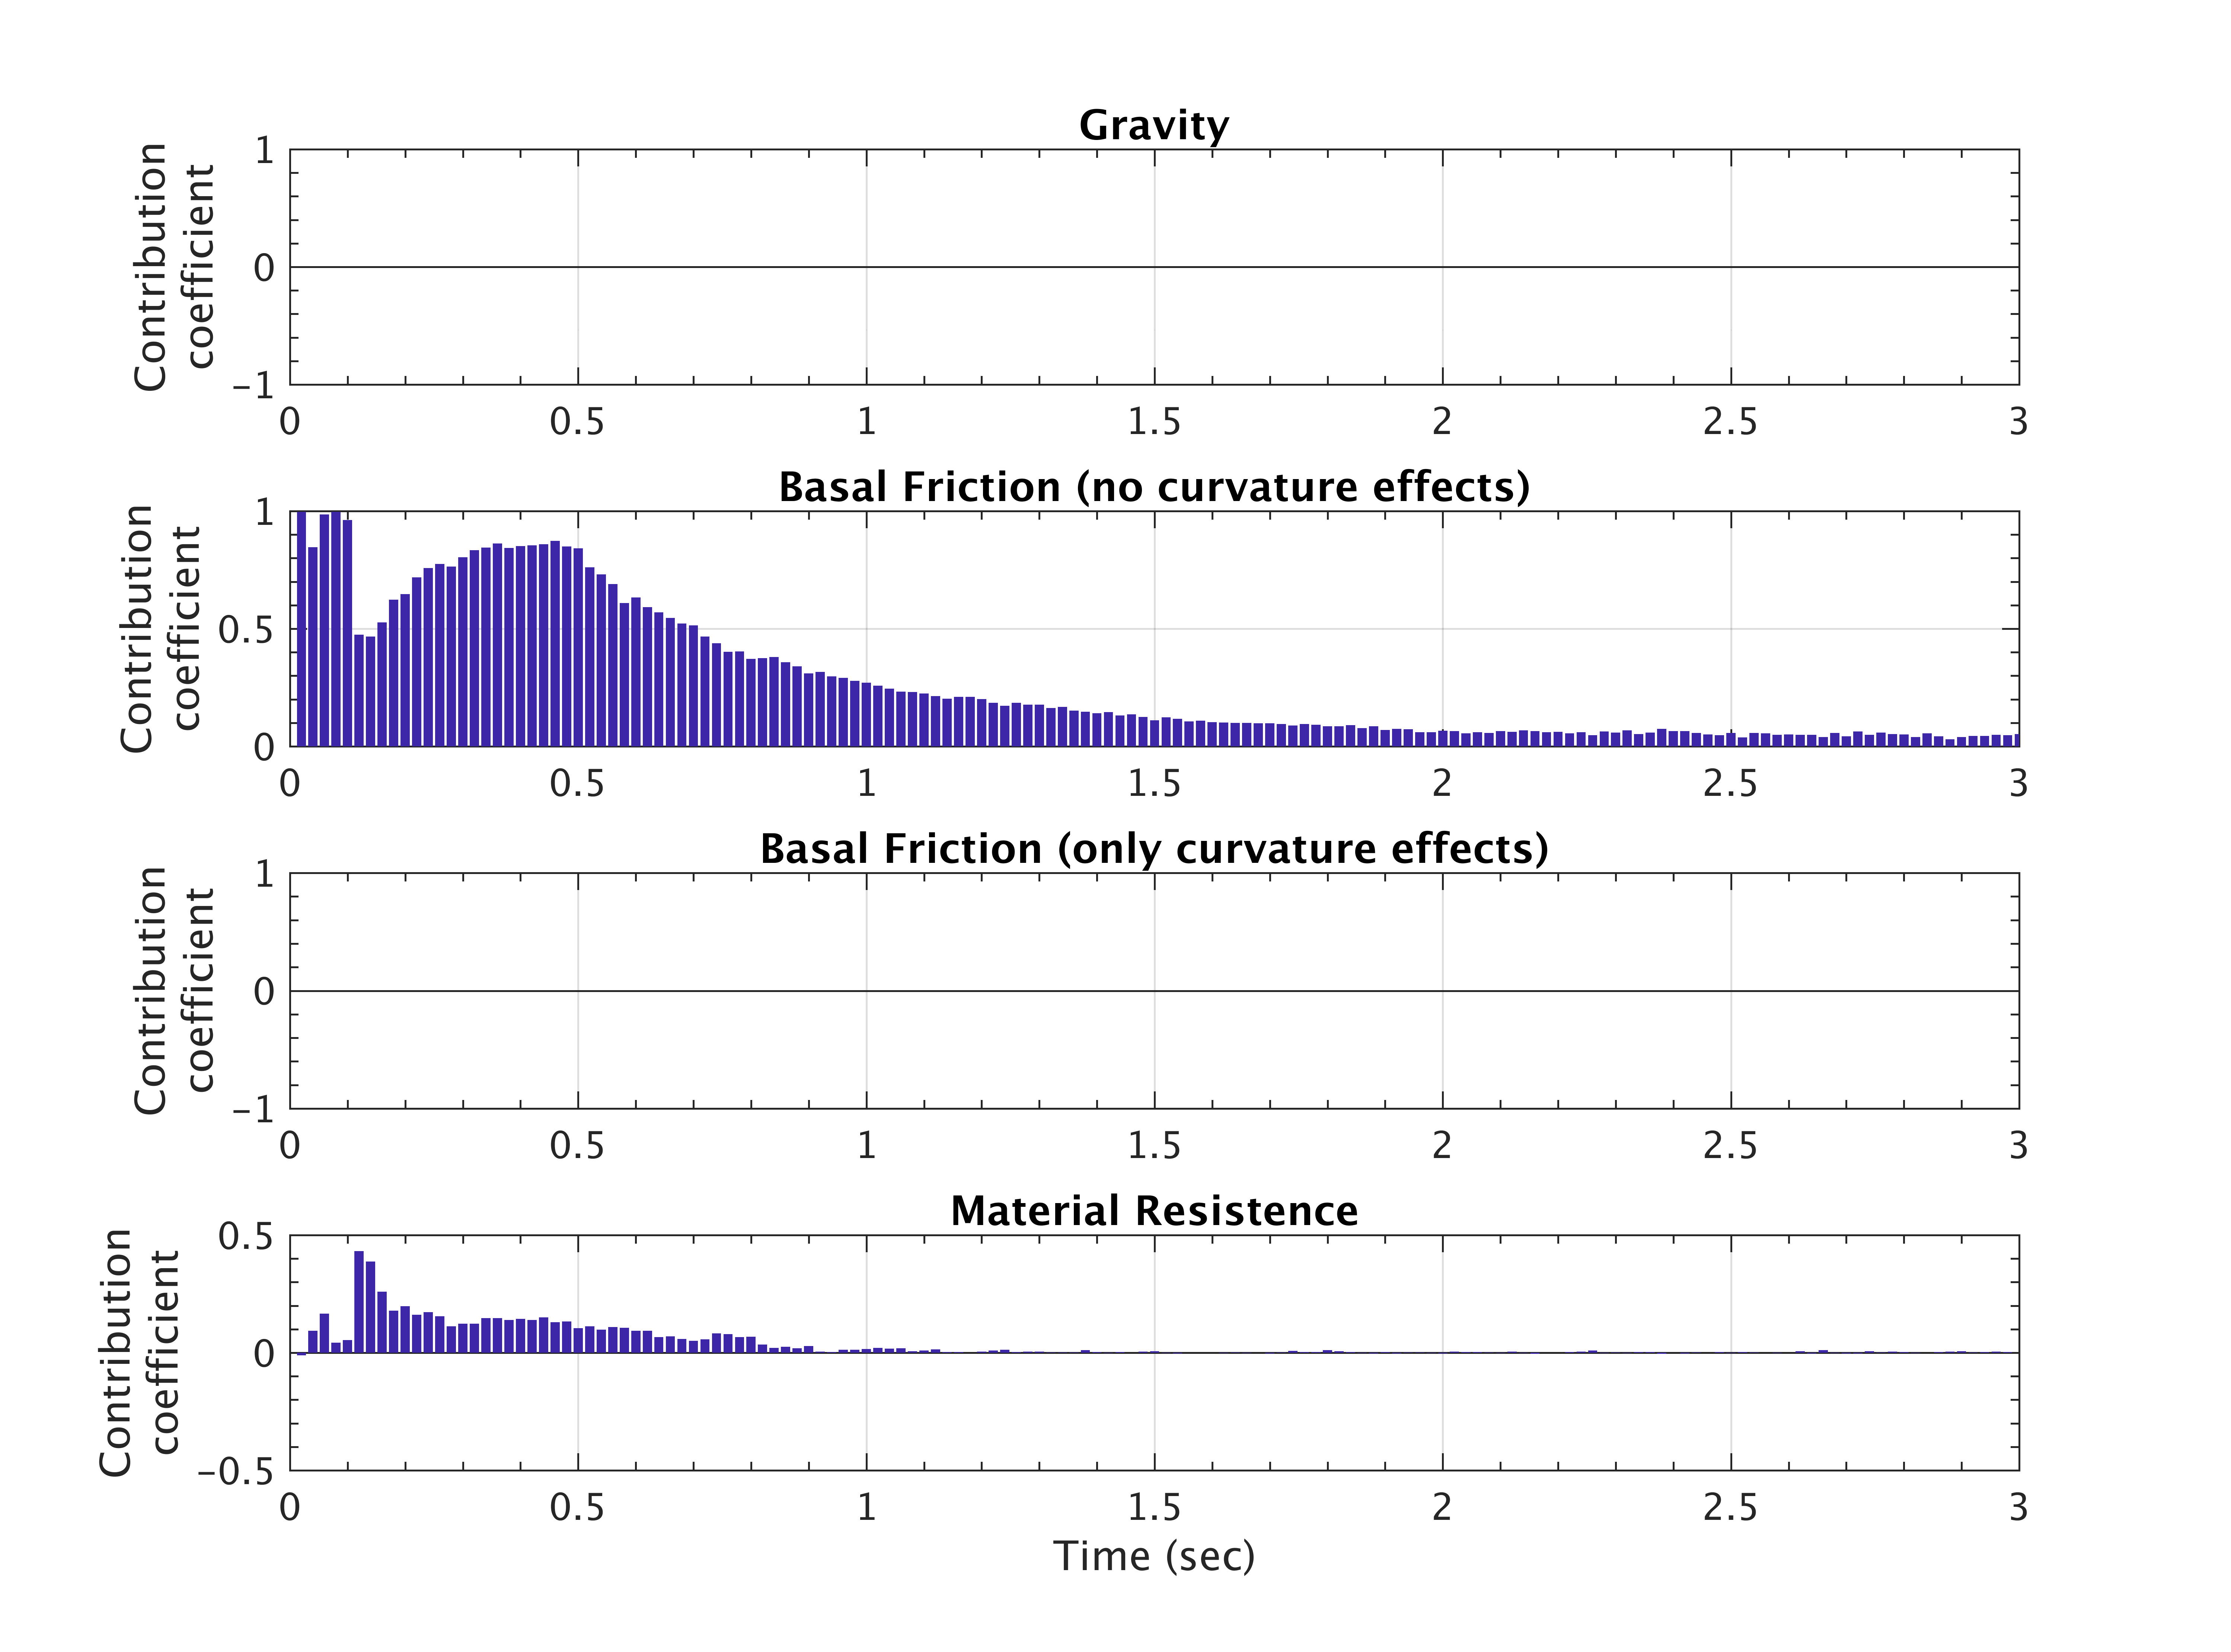
\includegraphics[width=1\textwidth]{InclinedPlane/LocalRecords/ContribF1_C_y.png}
                \subcaption{$x=-0.7, \ y=0.0$, slumping pile location.}
                \label{fig:Ramp-Cy1}
        \end{minipage}
        \begin{minipage}[b]{0.5\linewidth}
                \centering
                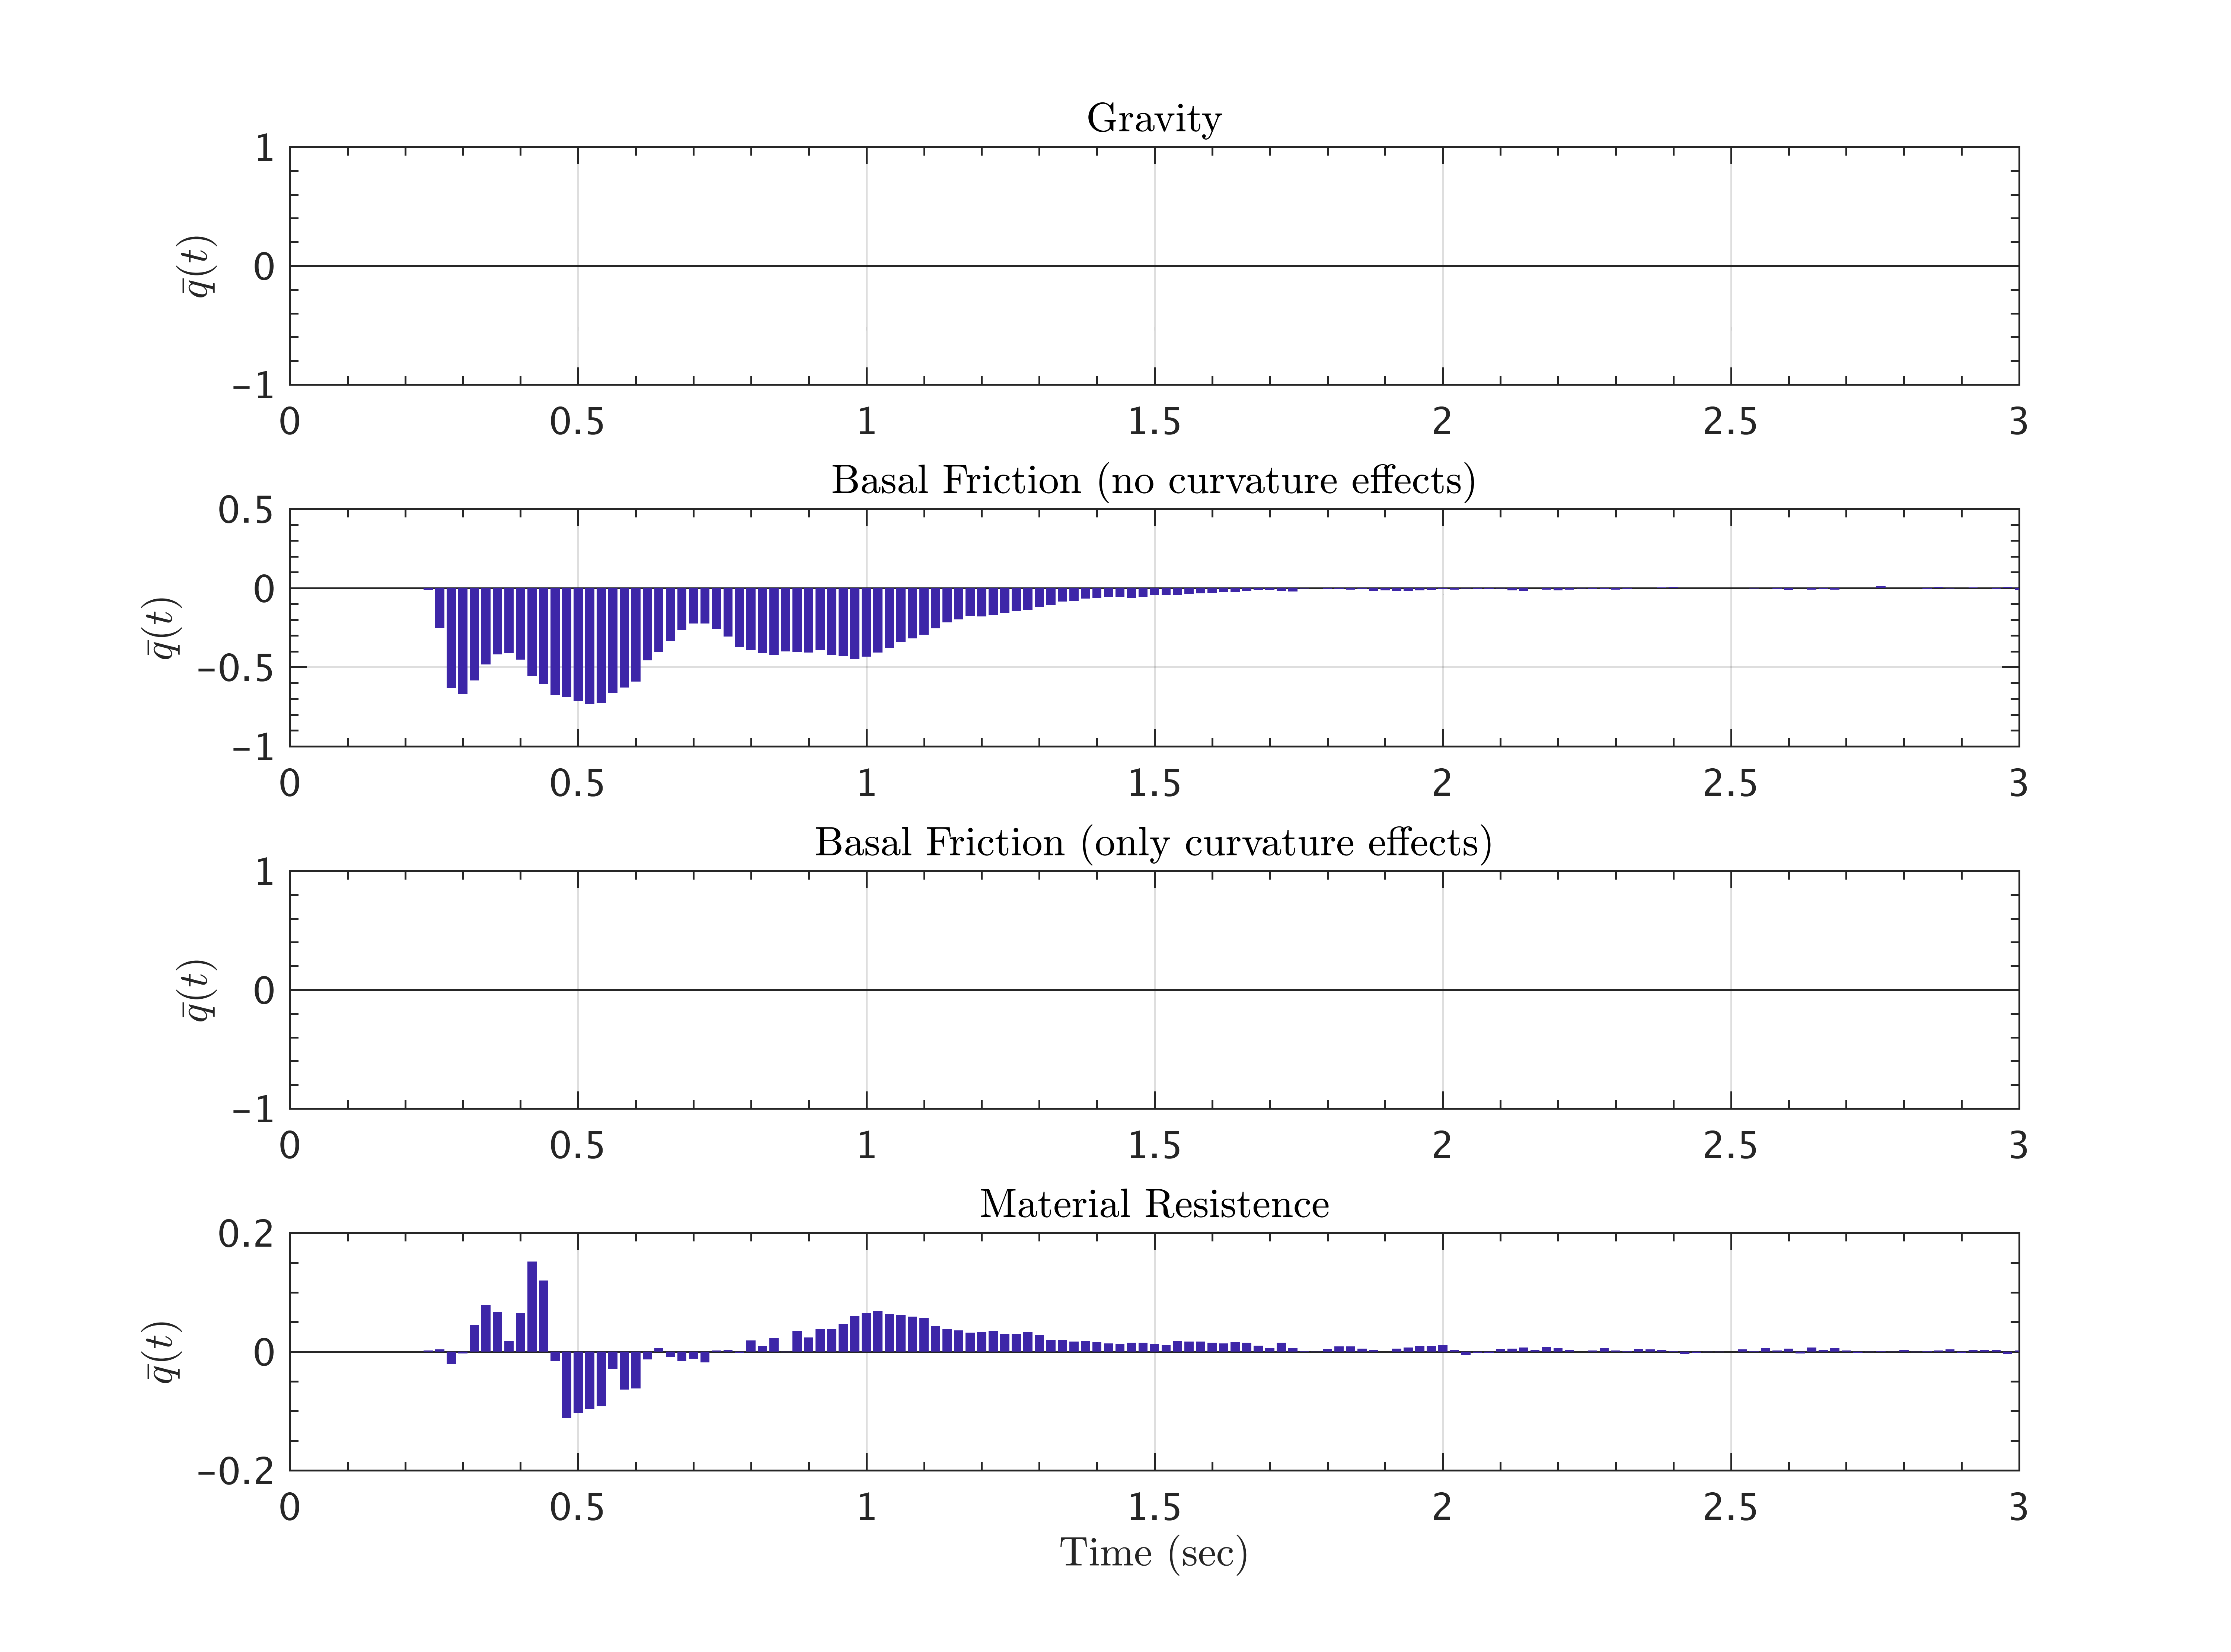
\includegraphics[width=1\textwidth]{InclinedPlane/LocalRecords/ContribF8_C_y.png}
                \subcaption{$x=-0.35, \ y=0.0$, middle point on inclined plane.}
                \label{fig:Ramp-Cy2}
        \end{minipage}

        \begin{minipage}[b]{0.5\linewidth}
                \centering
                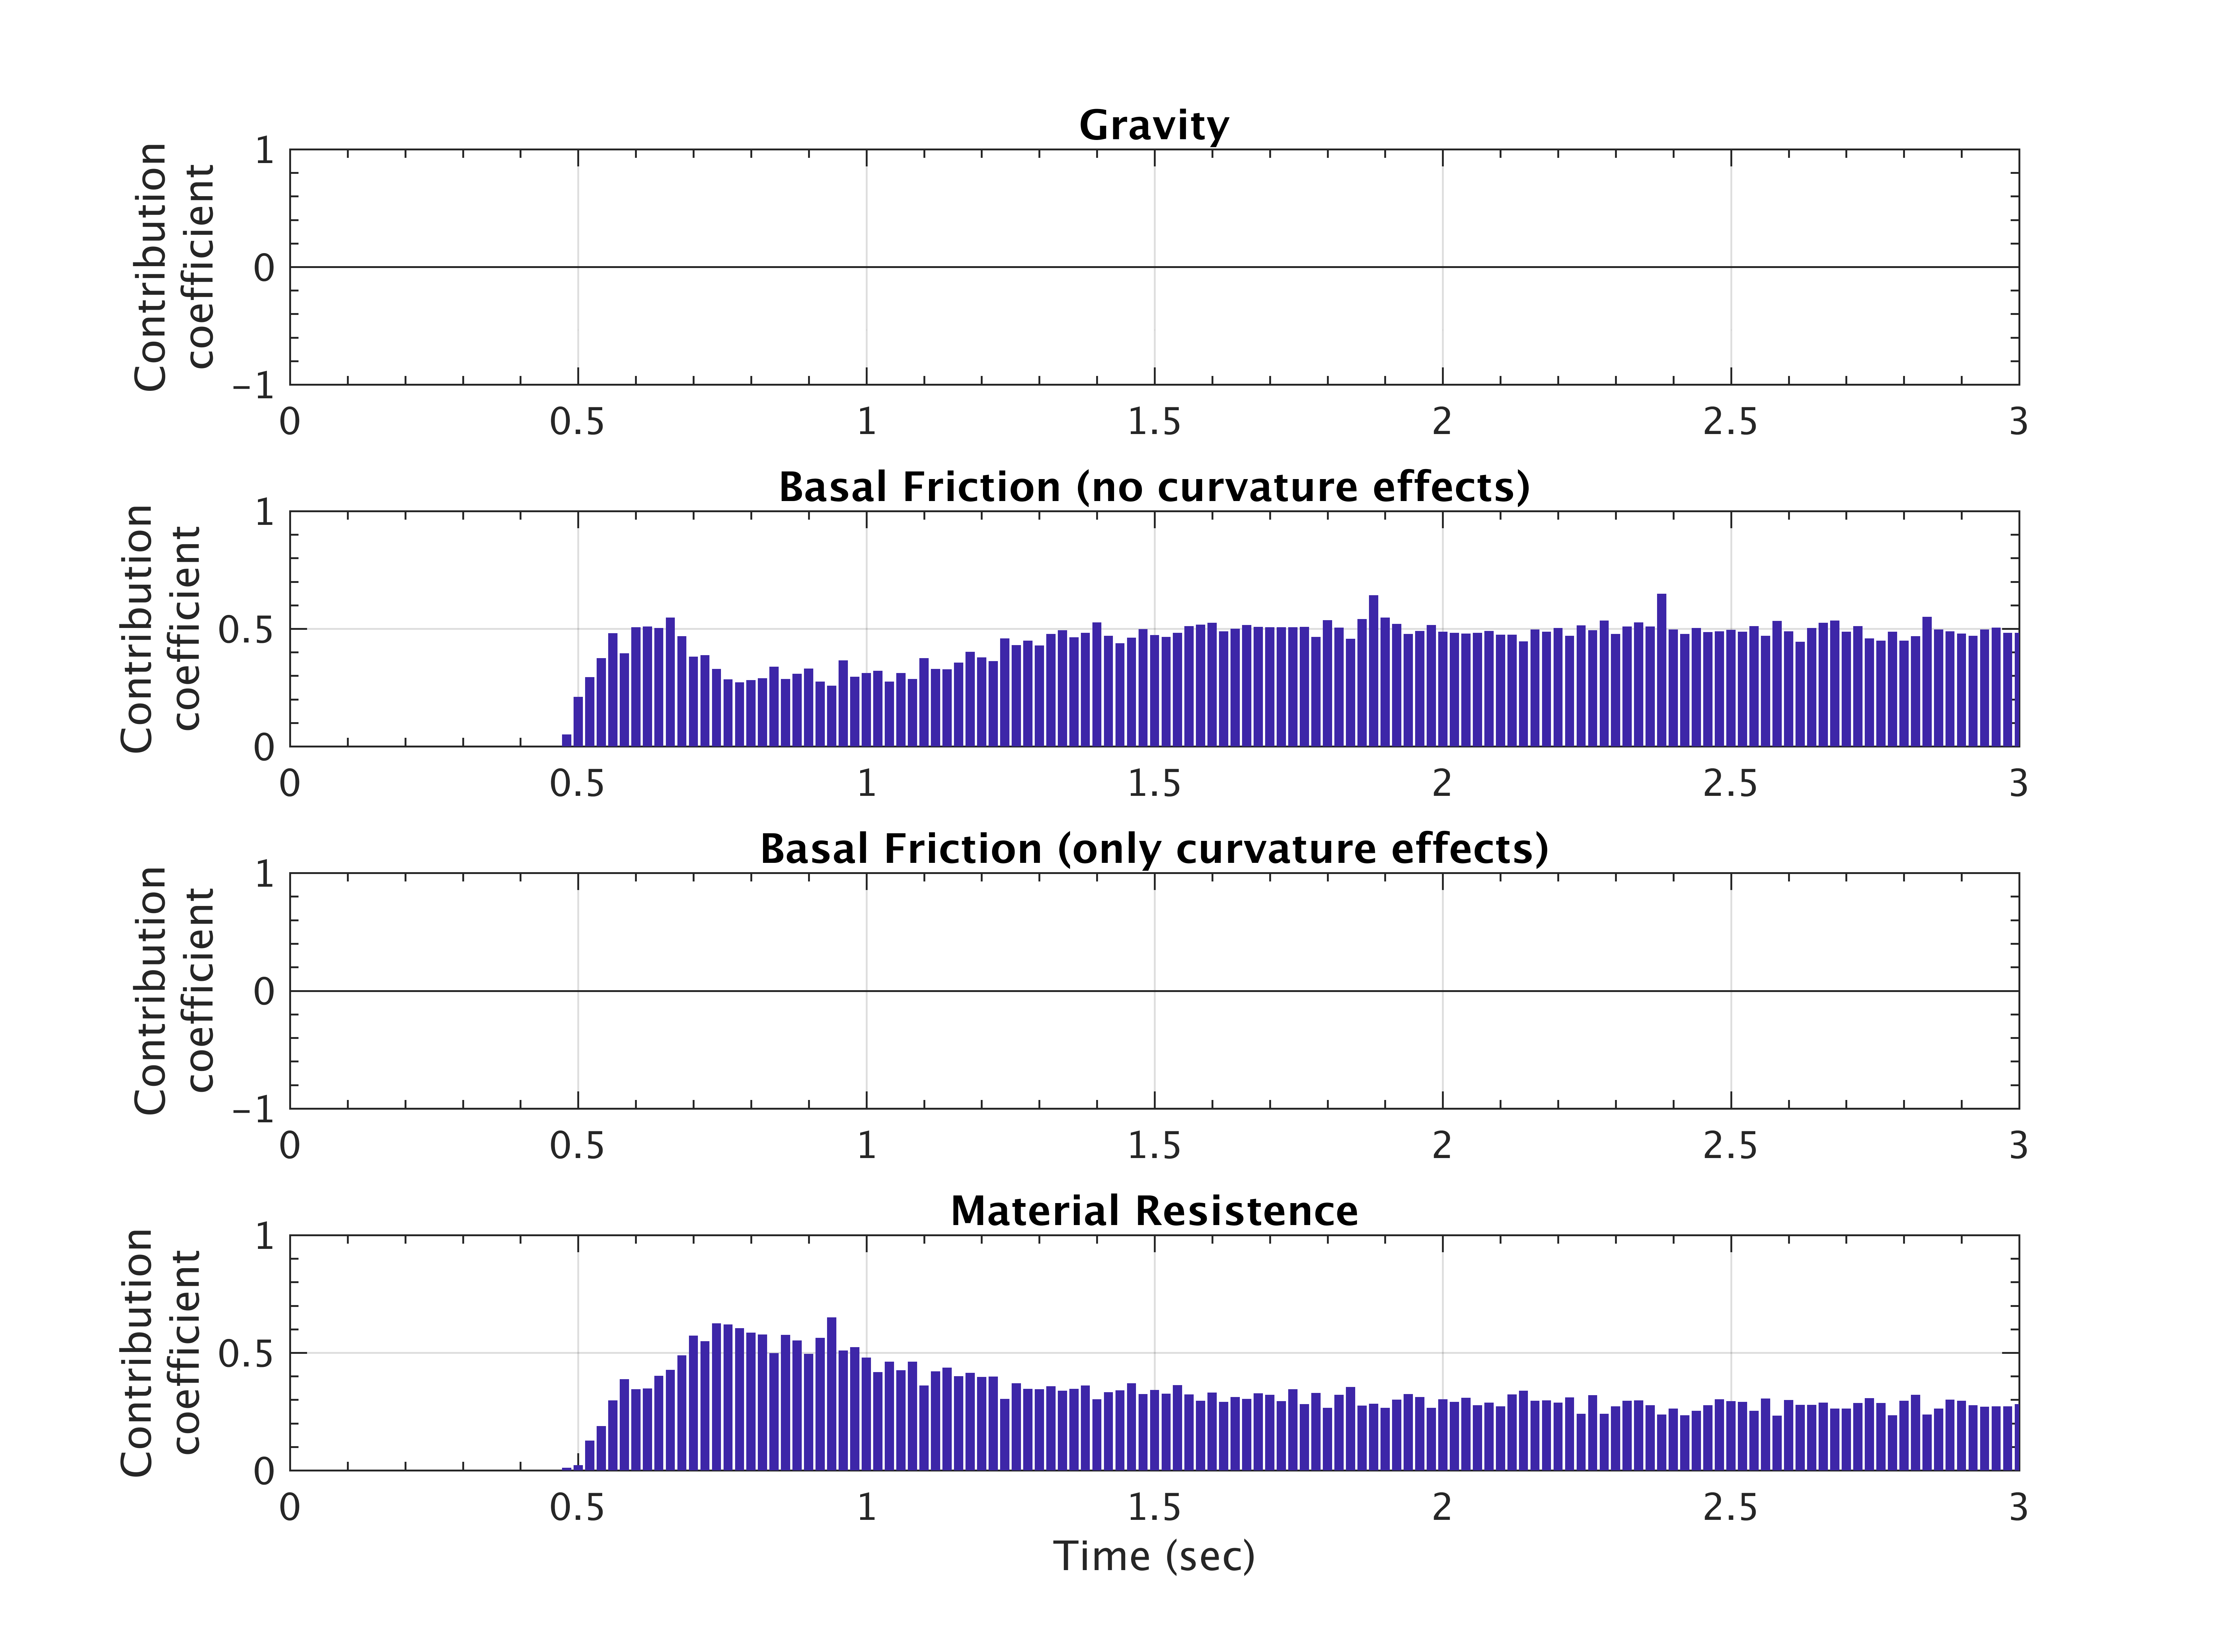
\includegraphics[width=1\textwidth]{InclinedPlane/LocalRecords/ContribF15_C_y.png}
                \subcaption{$x=0, \ y=0$, inclined and runout planes' joint location.}
                \label{fig:Ramp-Cy3}
        \end{minipage}
        \begin{minipage}[b]{0.5\linewidth}
                \centering
                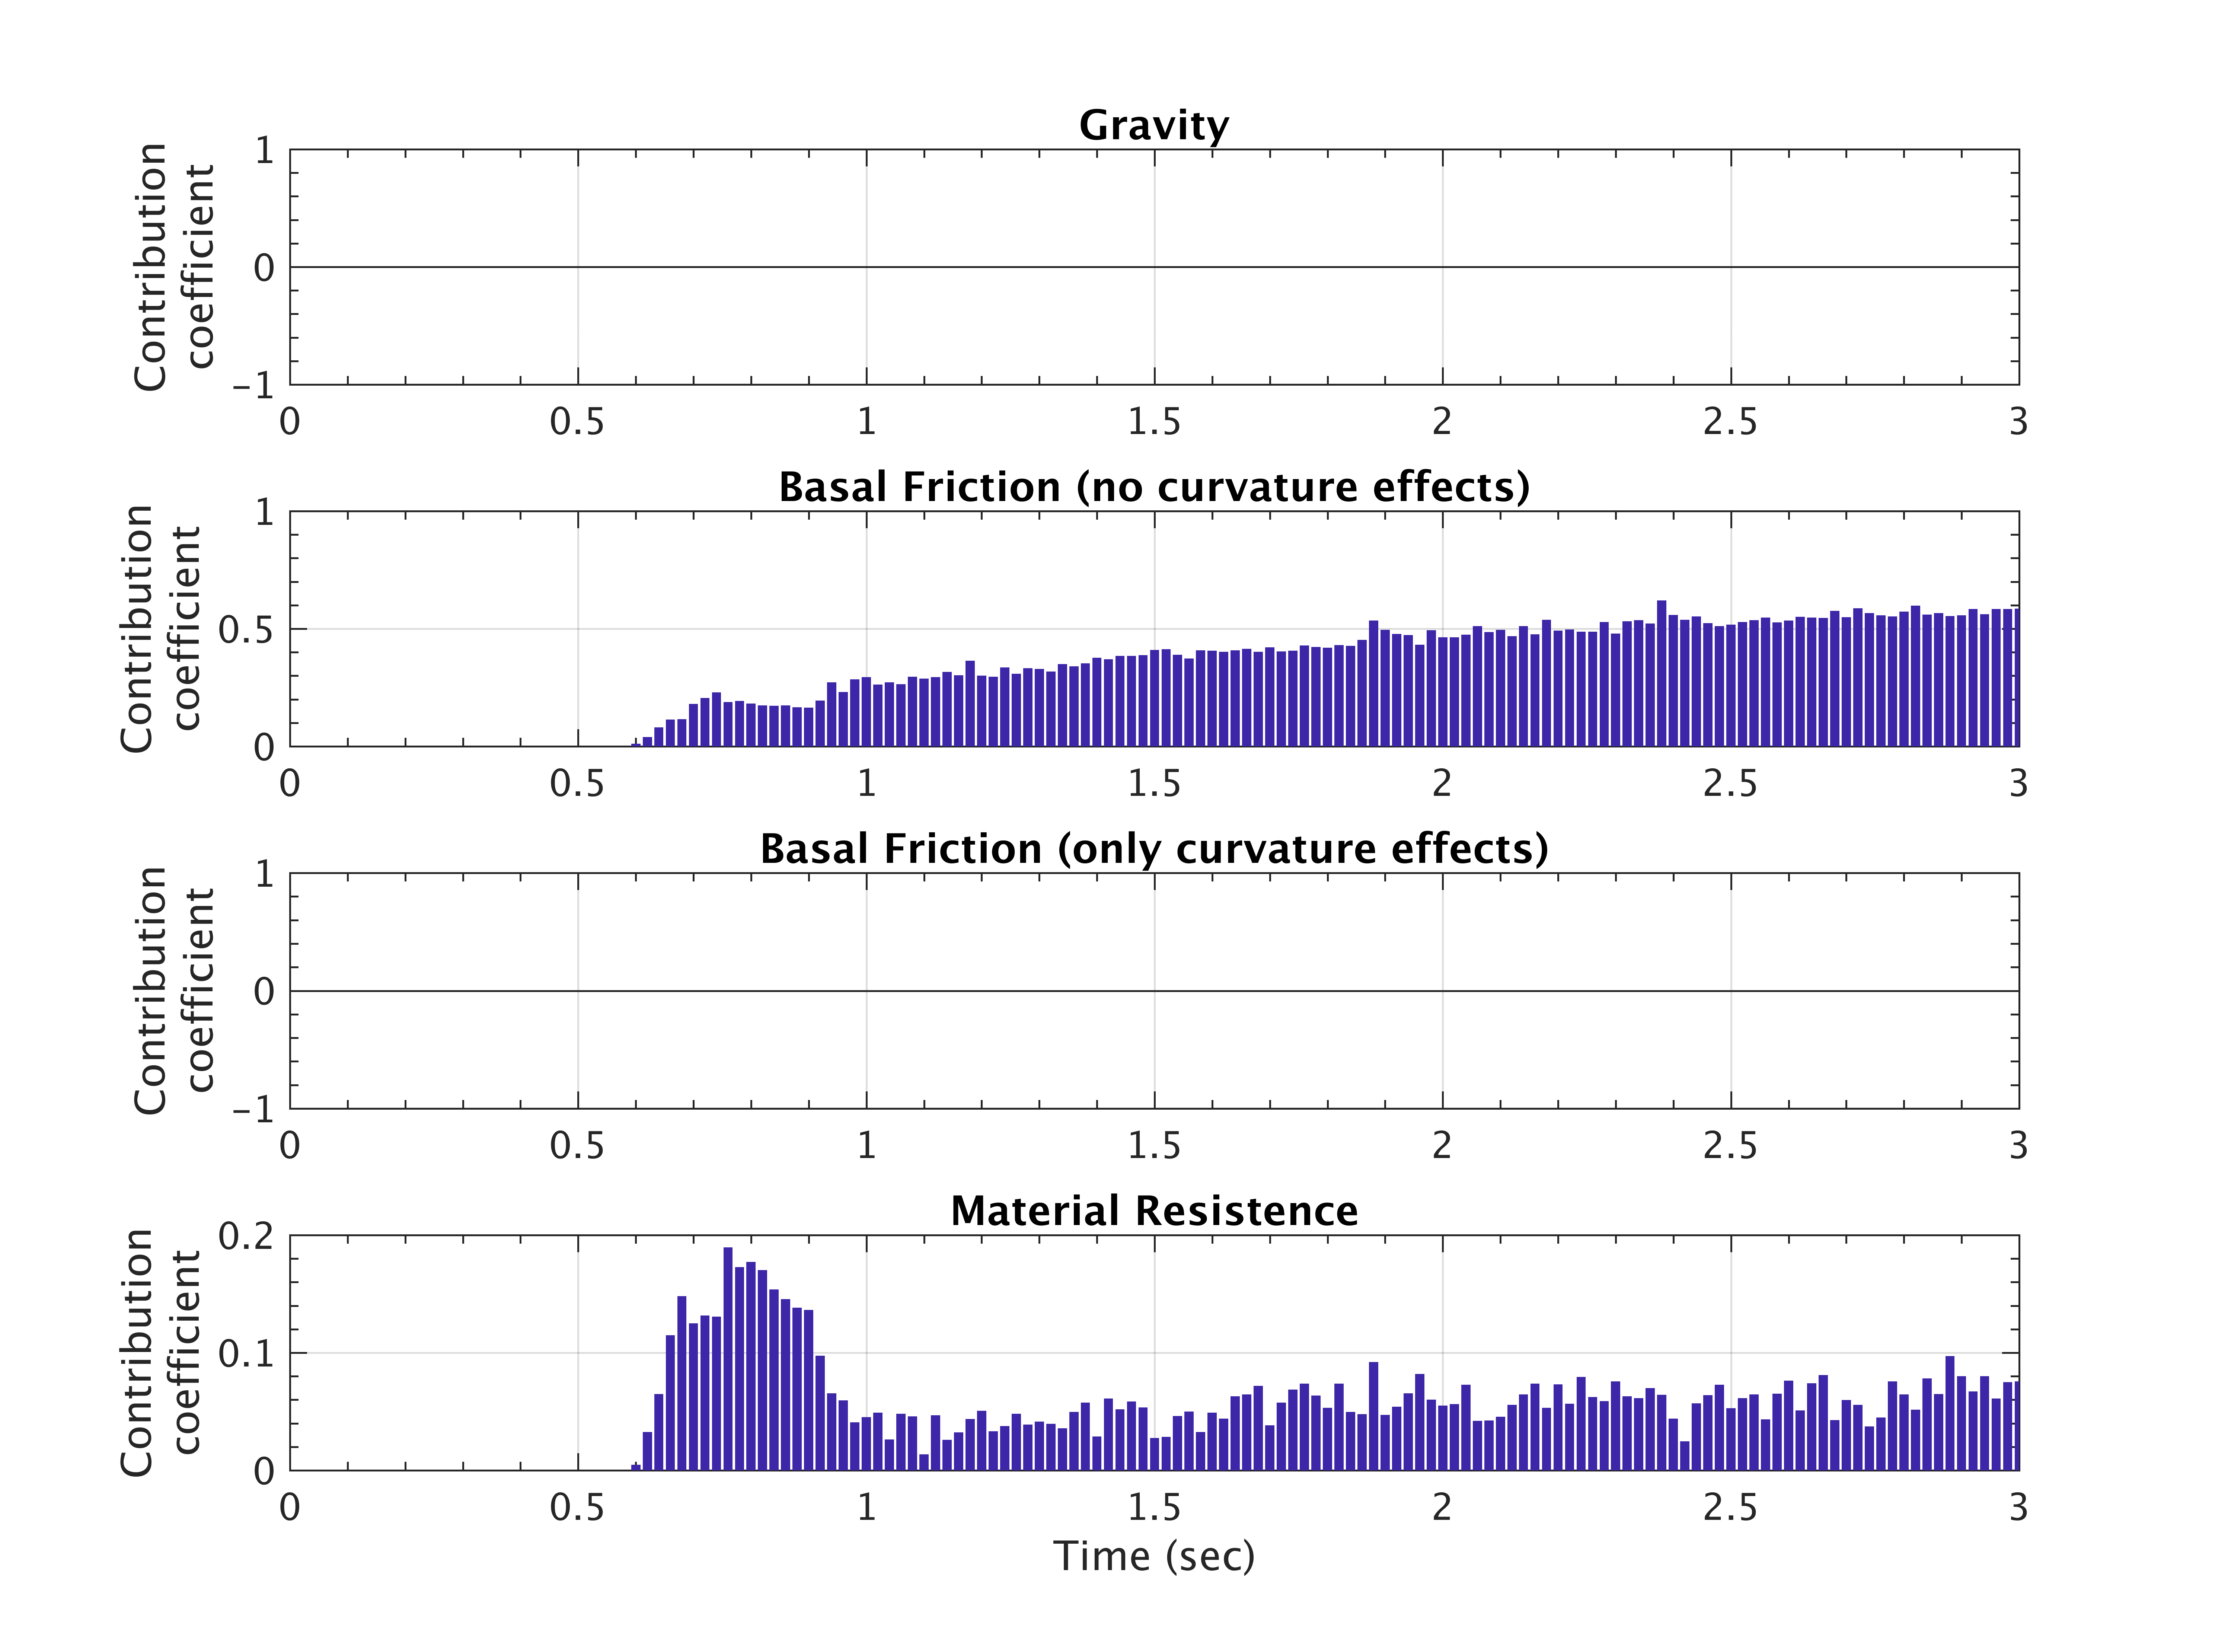
\includegraphics[width=1\textwidth]{InclinedPlane/LocalRecords/ContribF17_C_y.png}
                \subcaption{$x=0.15, \ y=0.0$, a location on runout plane.}
                \label{fig:Ramp-Cy4}
        \end{minipage}
        \caption{Time history of mean values for force impact quotients, $\bar{q}_i(t)$, along the lateral direction, Mohr-Coulomb model.}
        \label{fig:Ramp-Cy}
\end{figure}

\subsubsection{Pouliquen-Forterre Model, Force  Impact Quotients}
\begin{figure}[H]
        \begin{minipage}[b]{0.5\linewidth}
                \centering
                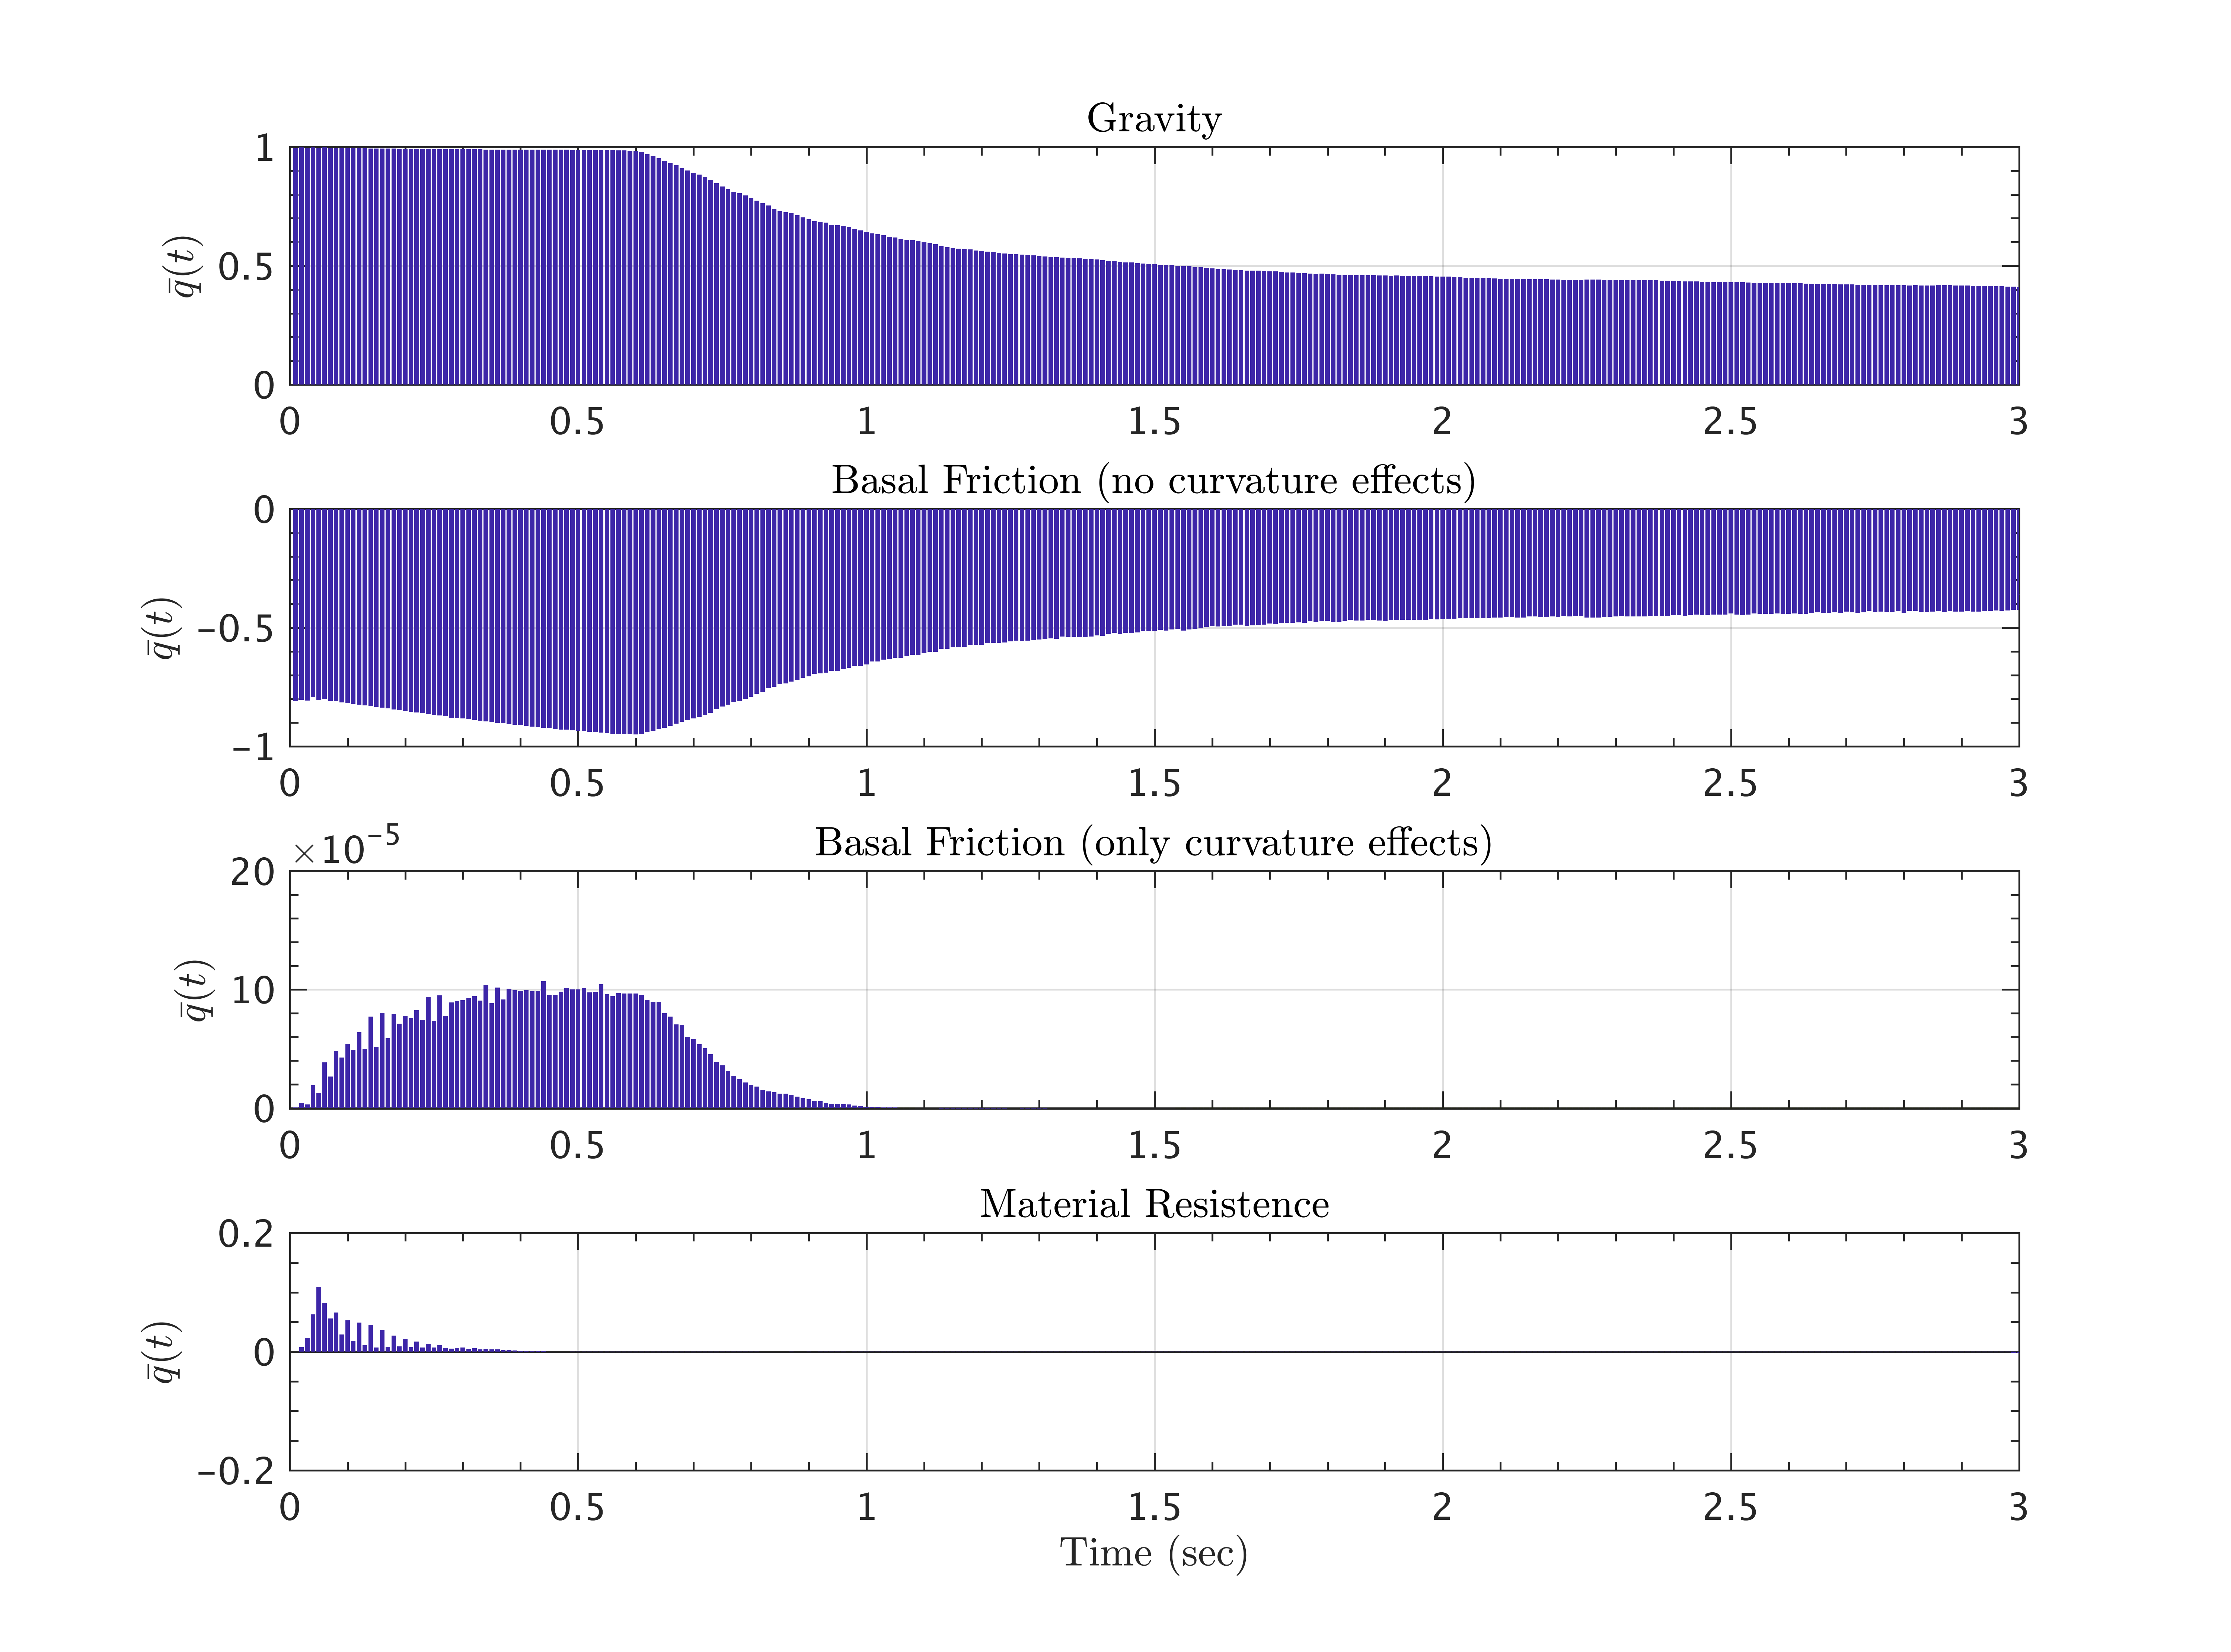
\includegraphics[width=1\textwidth]{InclinedPlane/LocalRecords/ContribF1_P_x.png}
                \subcaption{$x=-0.7, \ y=0.0$, slumping pile location.}
                \label{fig:Ramp-Px1}
        \end{minipage}
        \begin{minipage}[b]{0.5\linewidth}
                \centering
                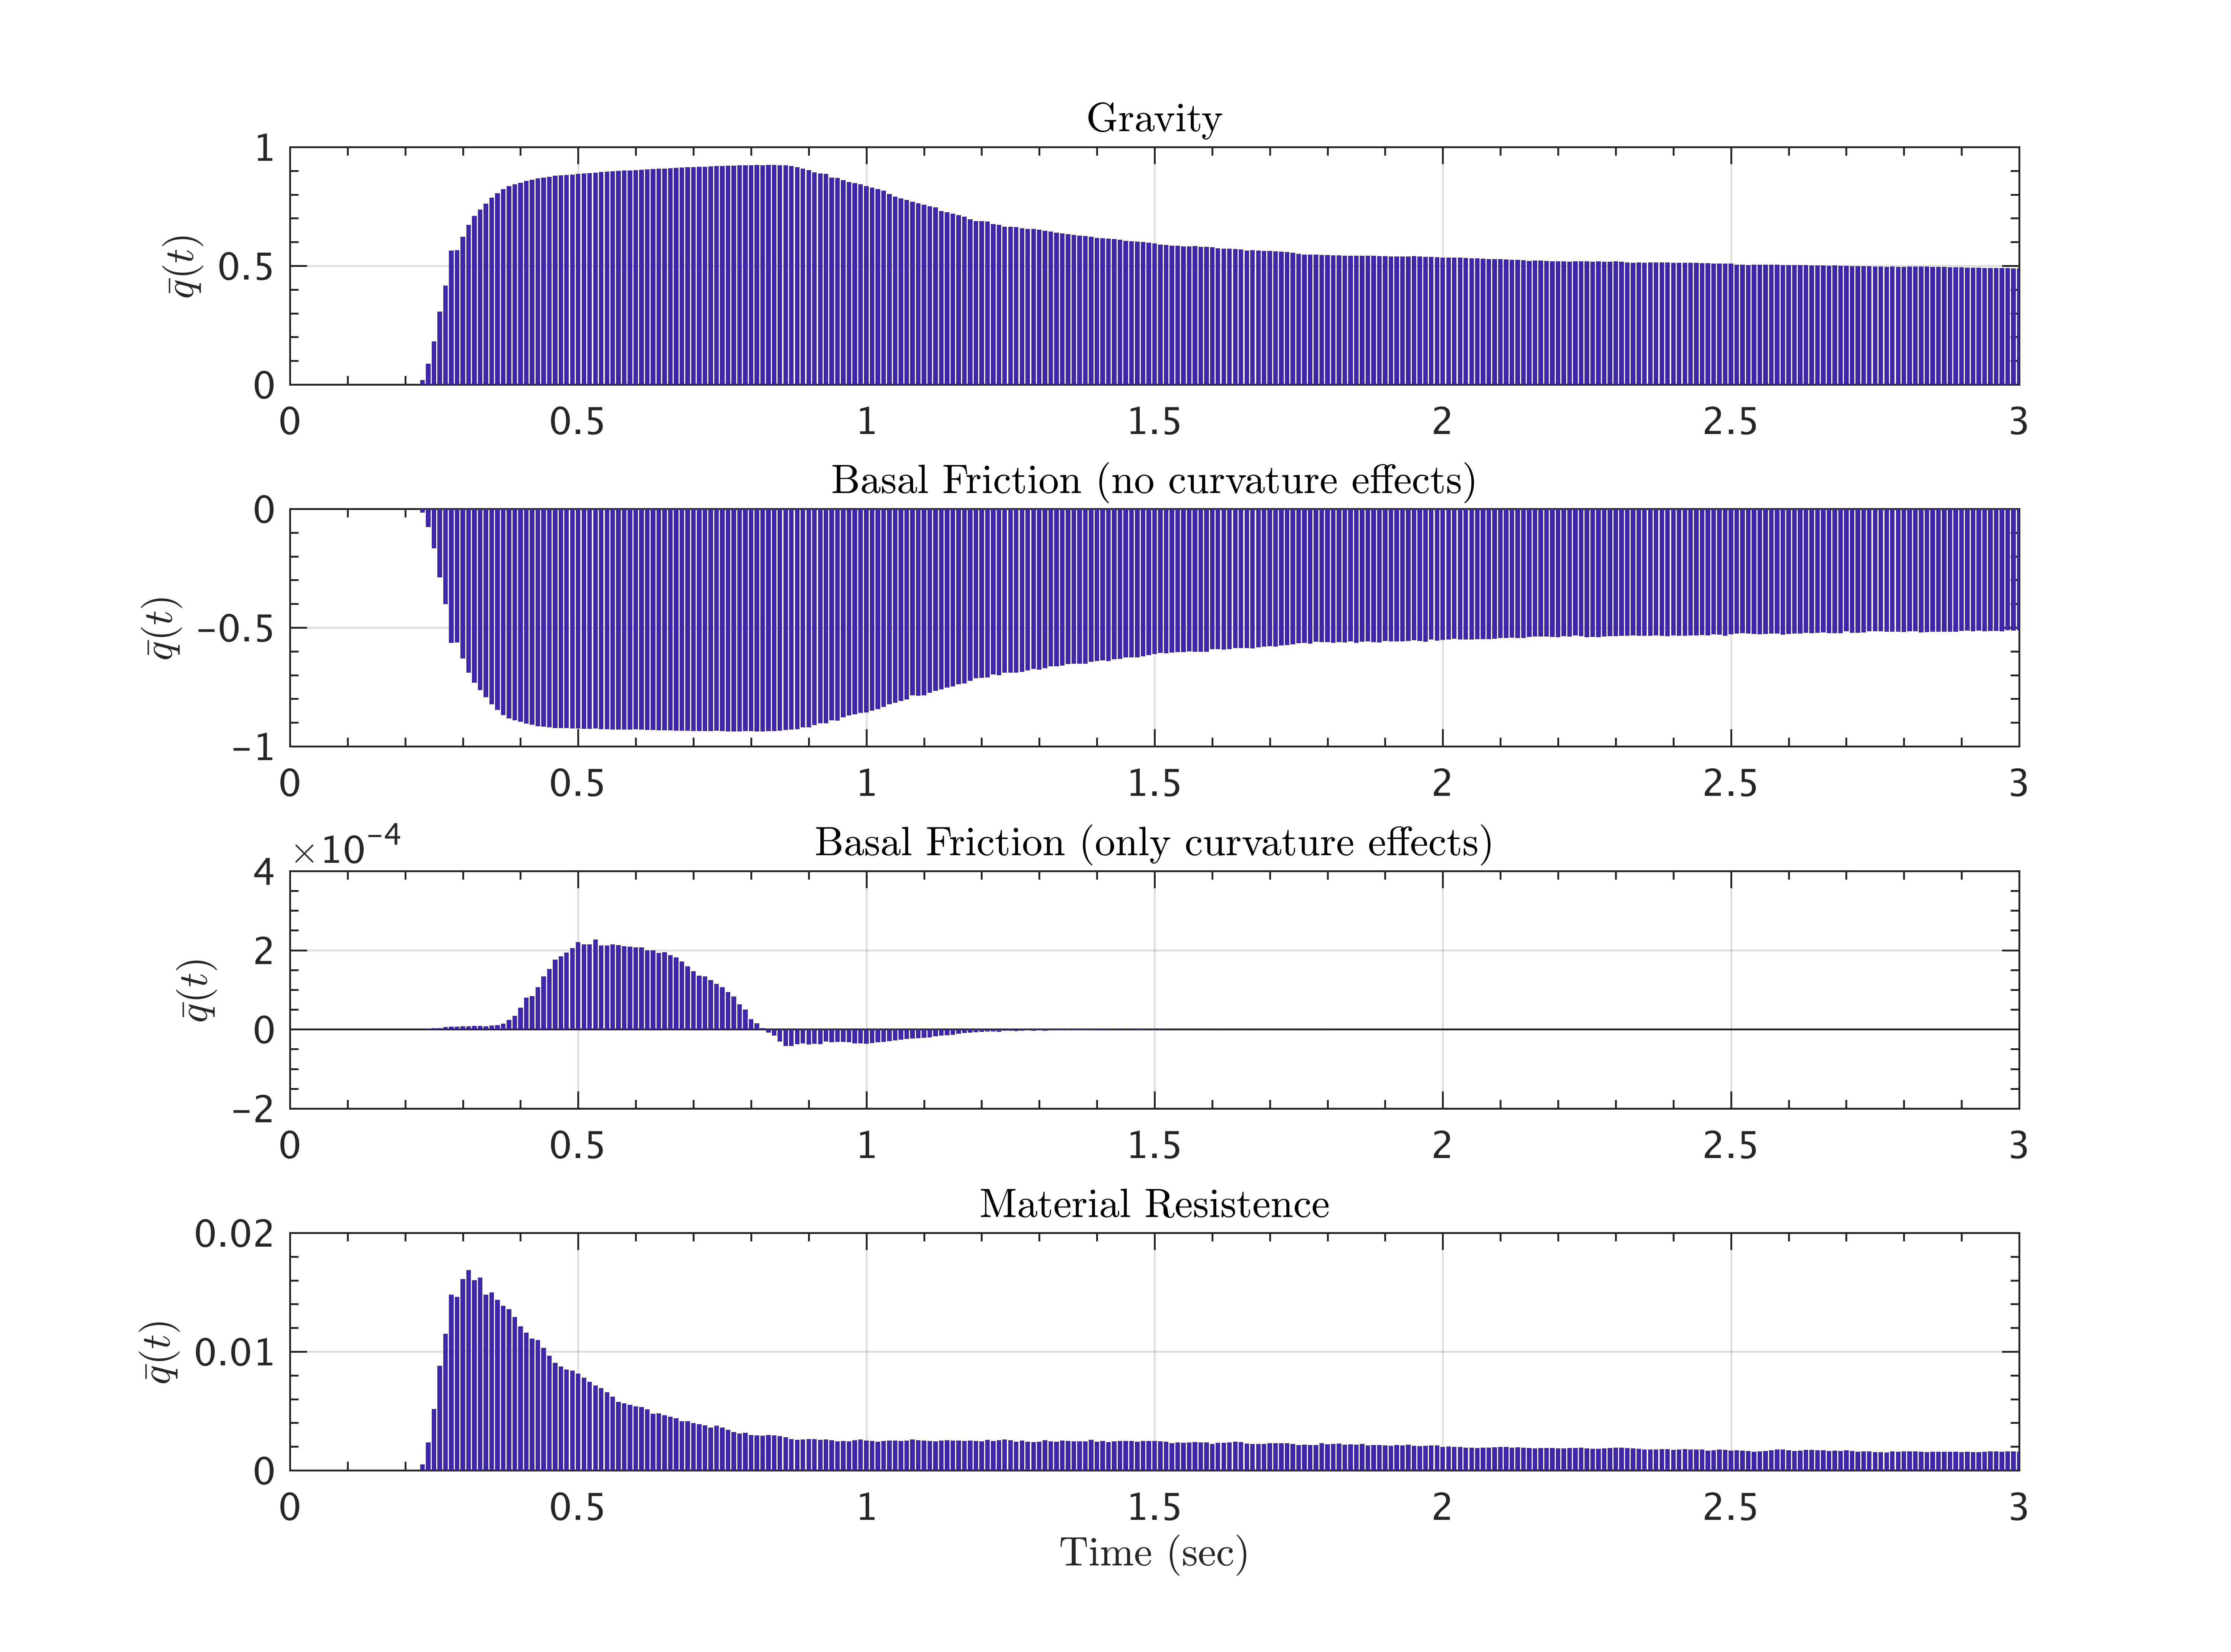
\includegraphics[width=1\textwidth]{InclinedPlane/LocalRecords/ContribF8_P_x.png}
                \subcaption{$x=-0.35, \ y=0.0$, middle point on inclined plane.}
                \label{fig:Ramp-Px2}
        \end{minipage}

        \begin{minipage}[b]{0.5\linewidth}
                \centering
                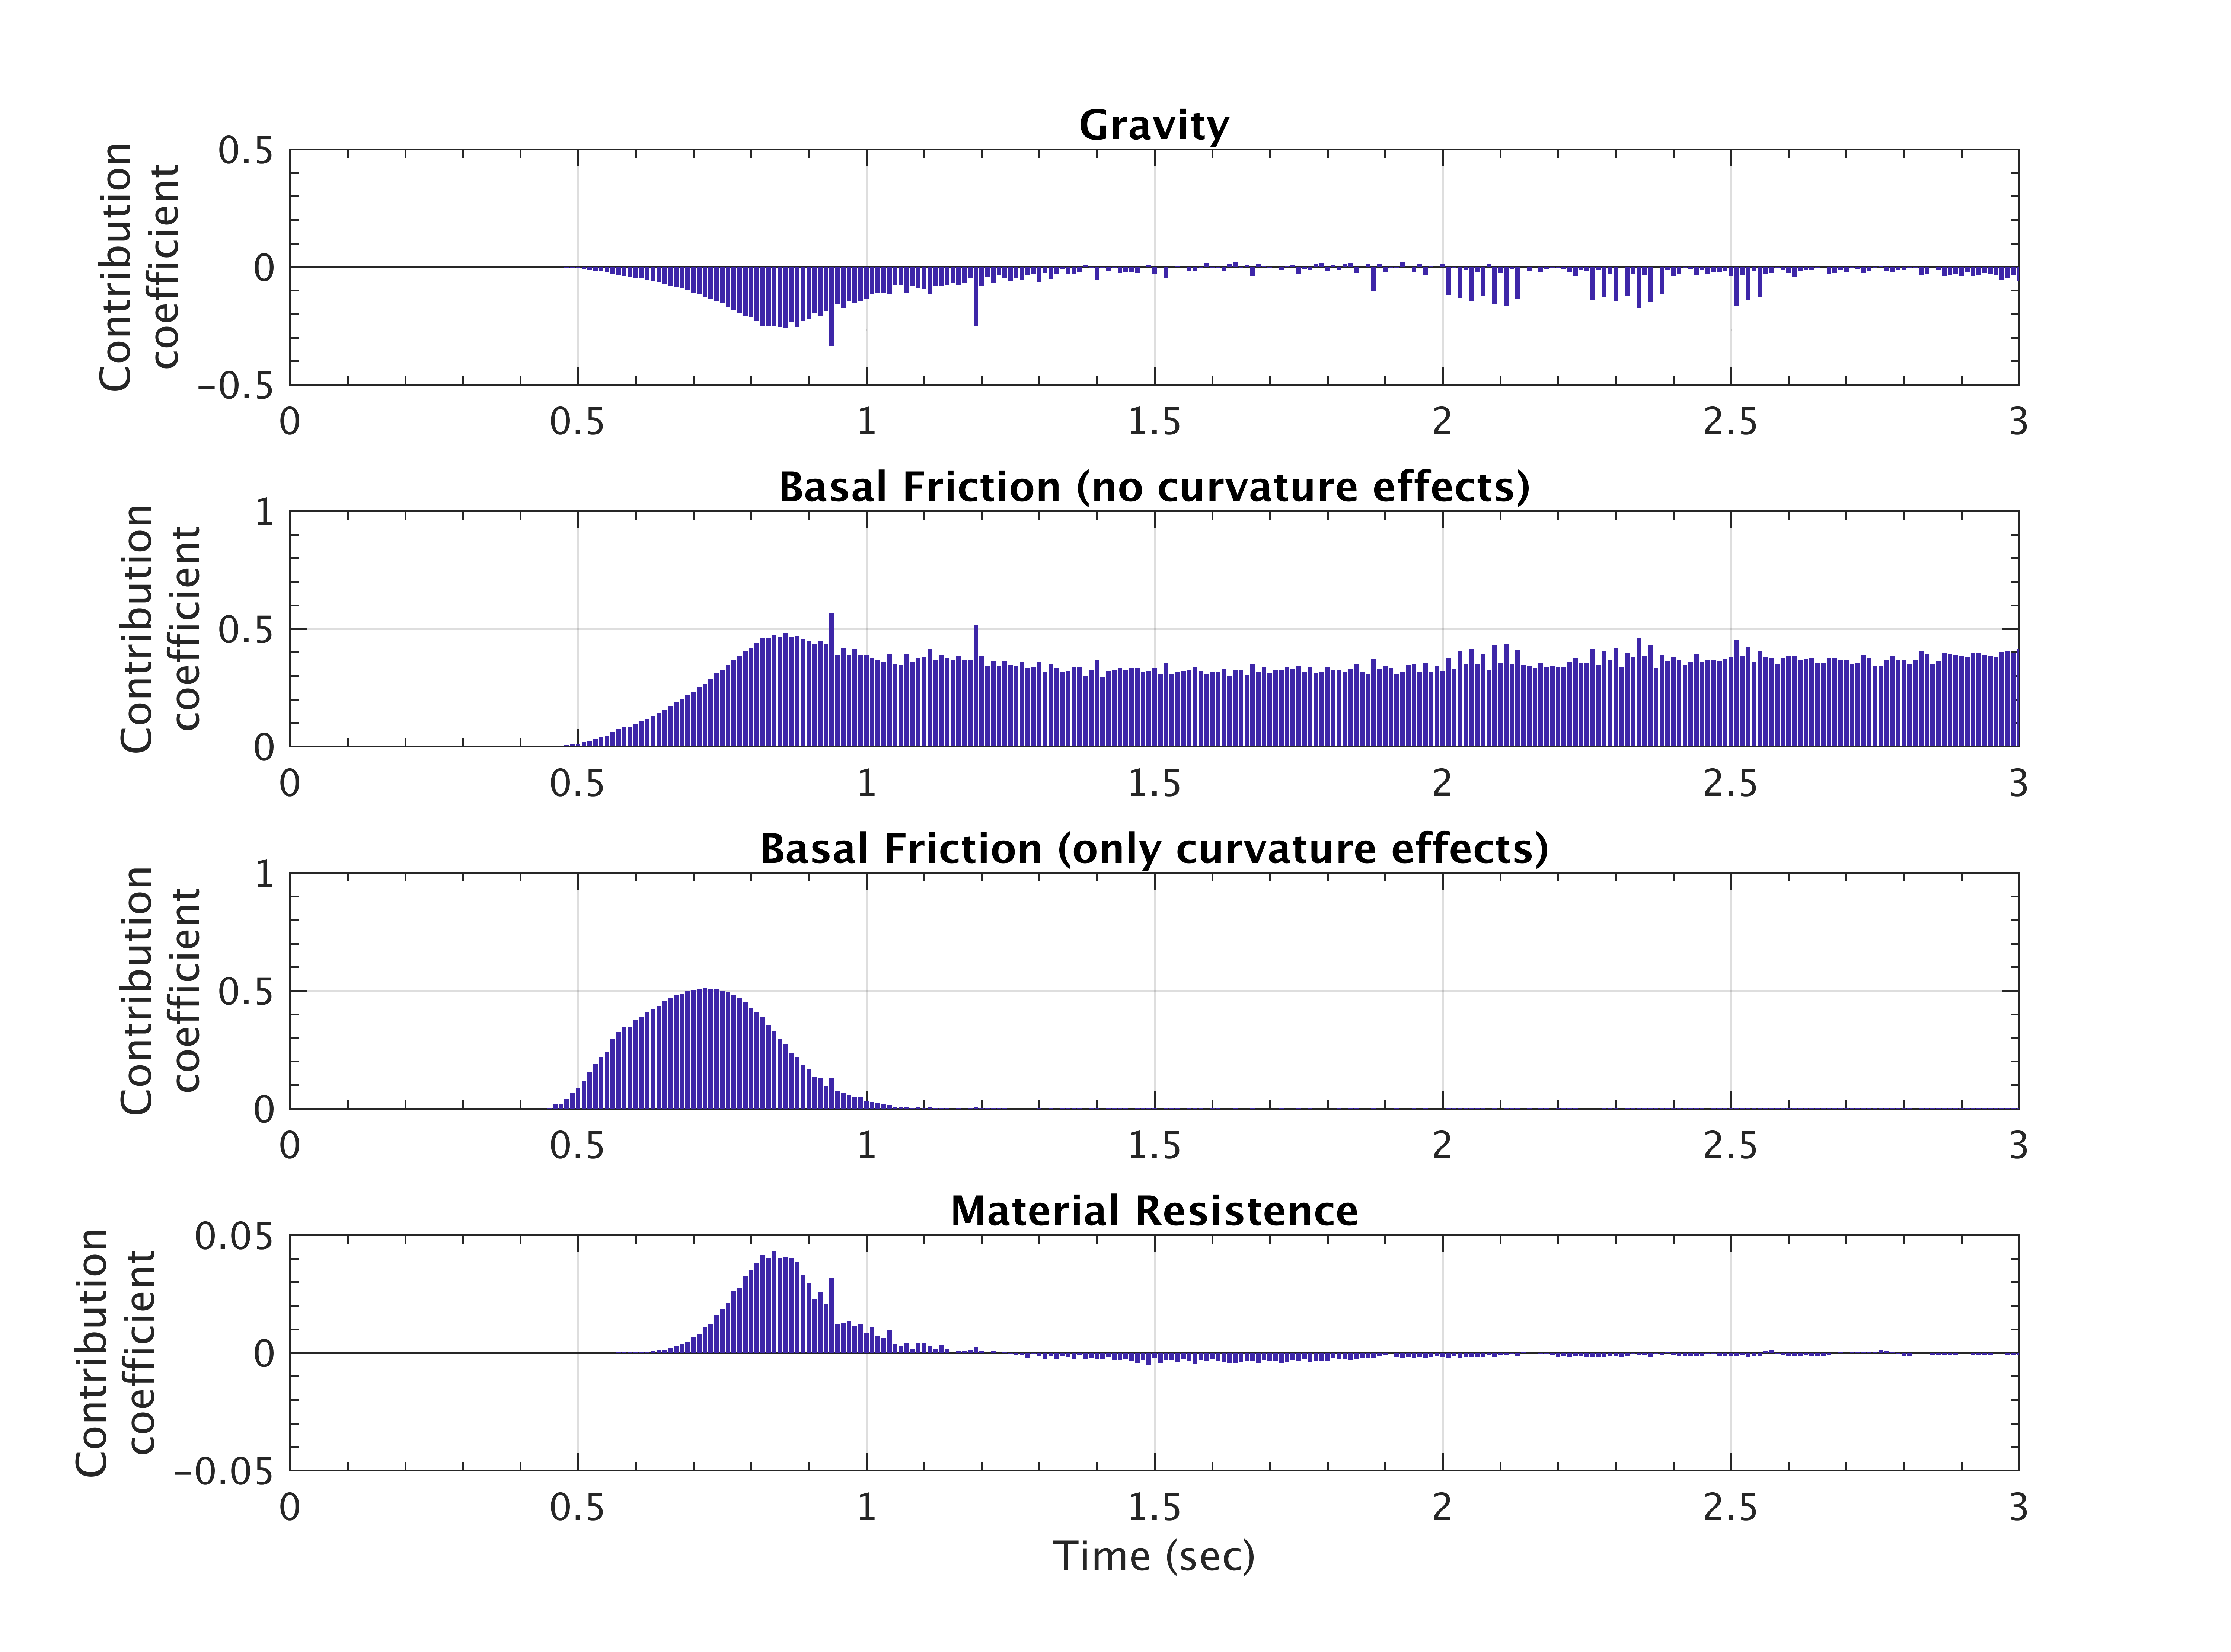
\includegraphics[width=1\textwidth]{InclinedPlane/LocalRecords/ContribF15_P_x.png}
                \subcaption{$x=0, \ y=0$, inclined and runout planes' joint location.}
                \label{fig:Ramp-Px3}
        \end{minipage}
        \begin{minipage}[b]{0.5\linewidth}
                \centering
                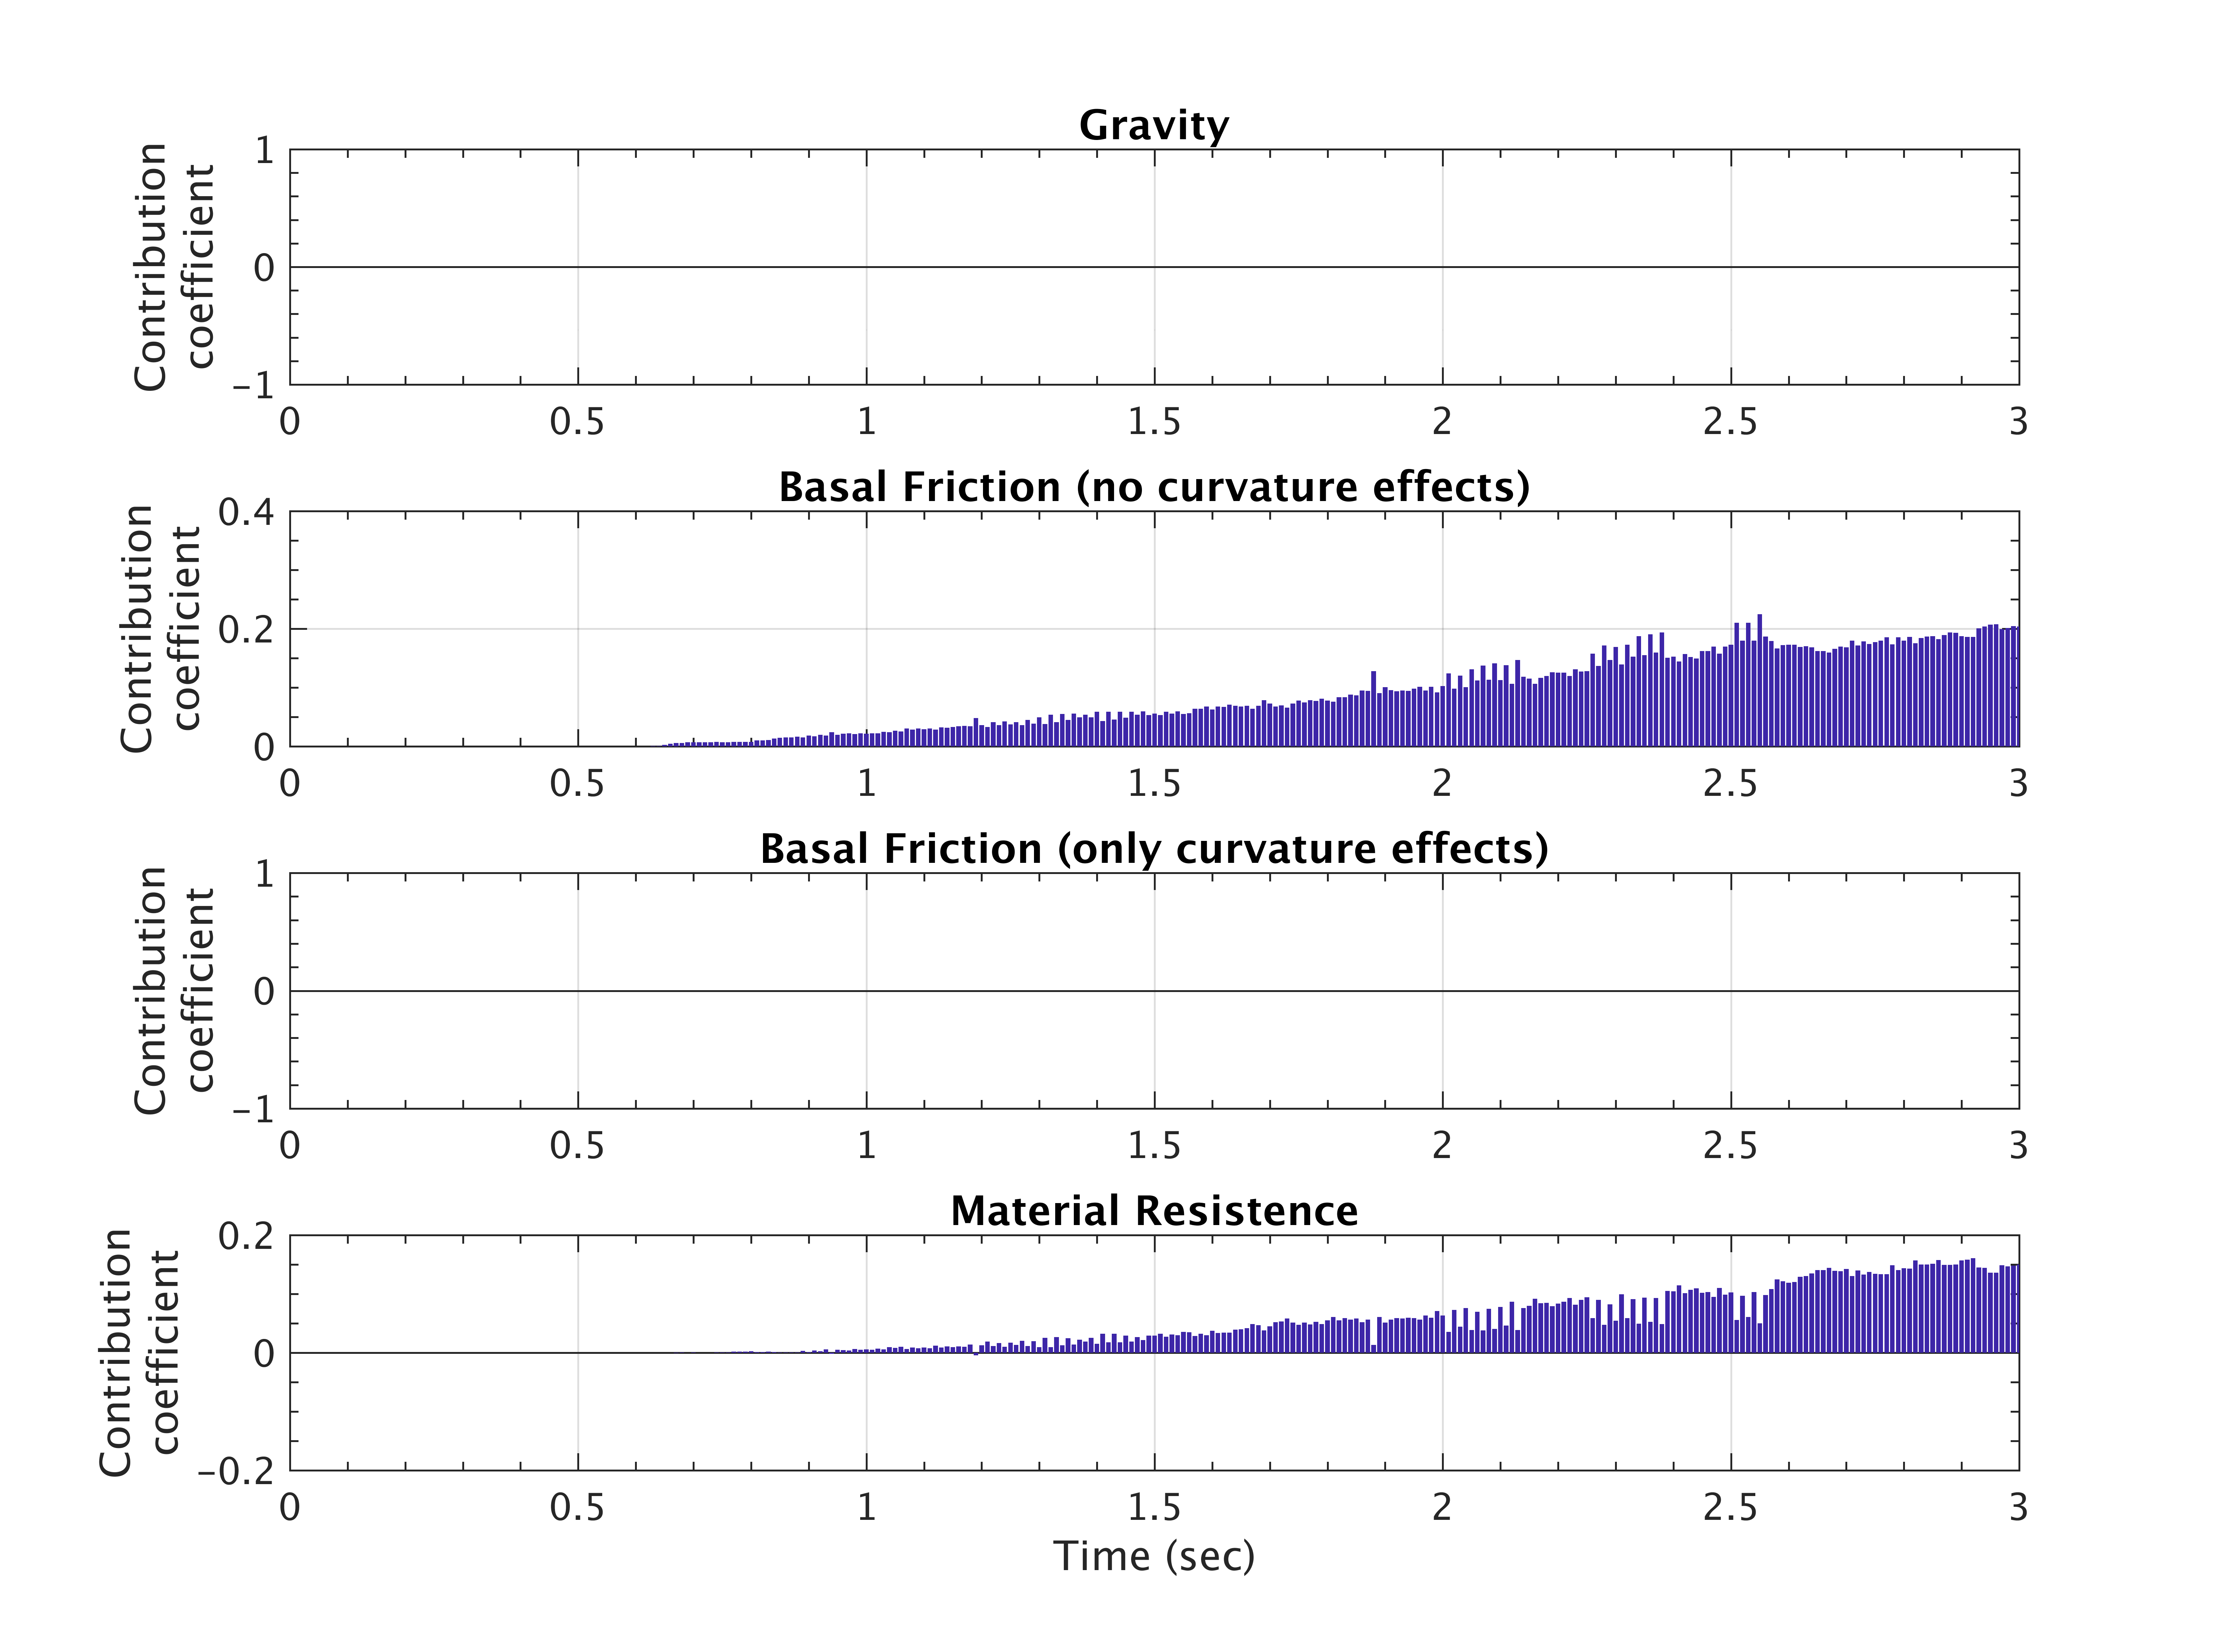
\includegraphics[width=1\textwidth]{InclinedPlane/LocalRecords/ContribF17_P_x.png}
                \subcaption{$x=0.15, \ y=0.0$, a location on runout plane.}
                \label{fig:Ramp-Px4}
        \end{minipage}
        \caption{Time history of mean values for force impact quotients, $\bar{q}_i(t)$, along runout direction, Pouliquen-Forterre model.}
        \label{fig:Ramp-Px}
\end{figure}

\begin{figure}[H]
        \begin{minipage}[b]{0.5\linewidth}
                \centering
                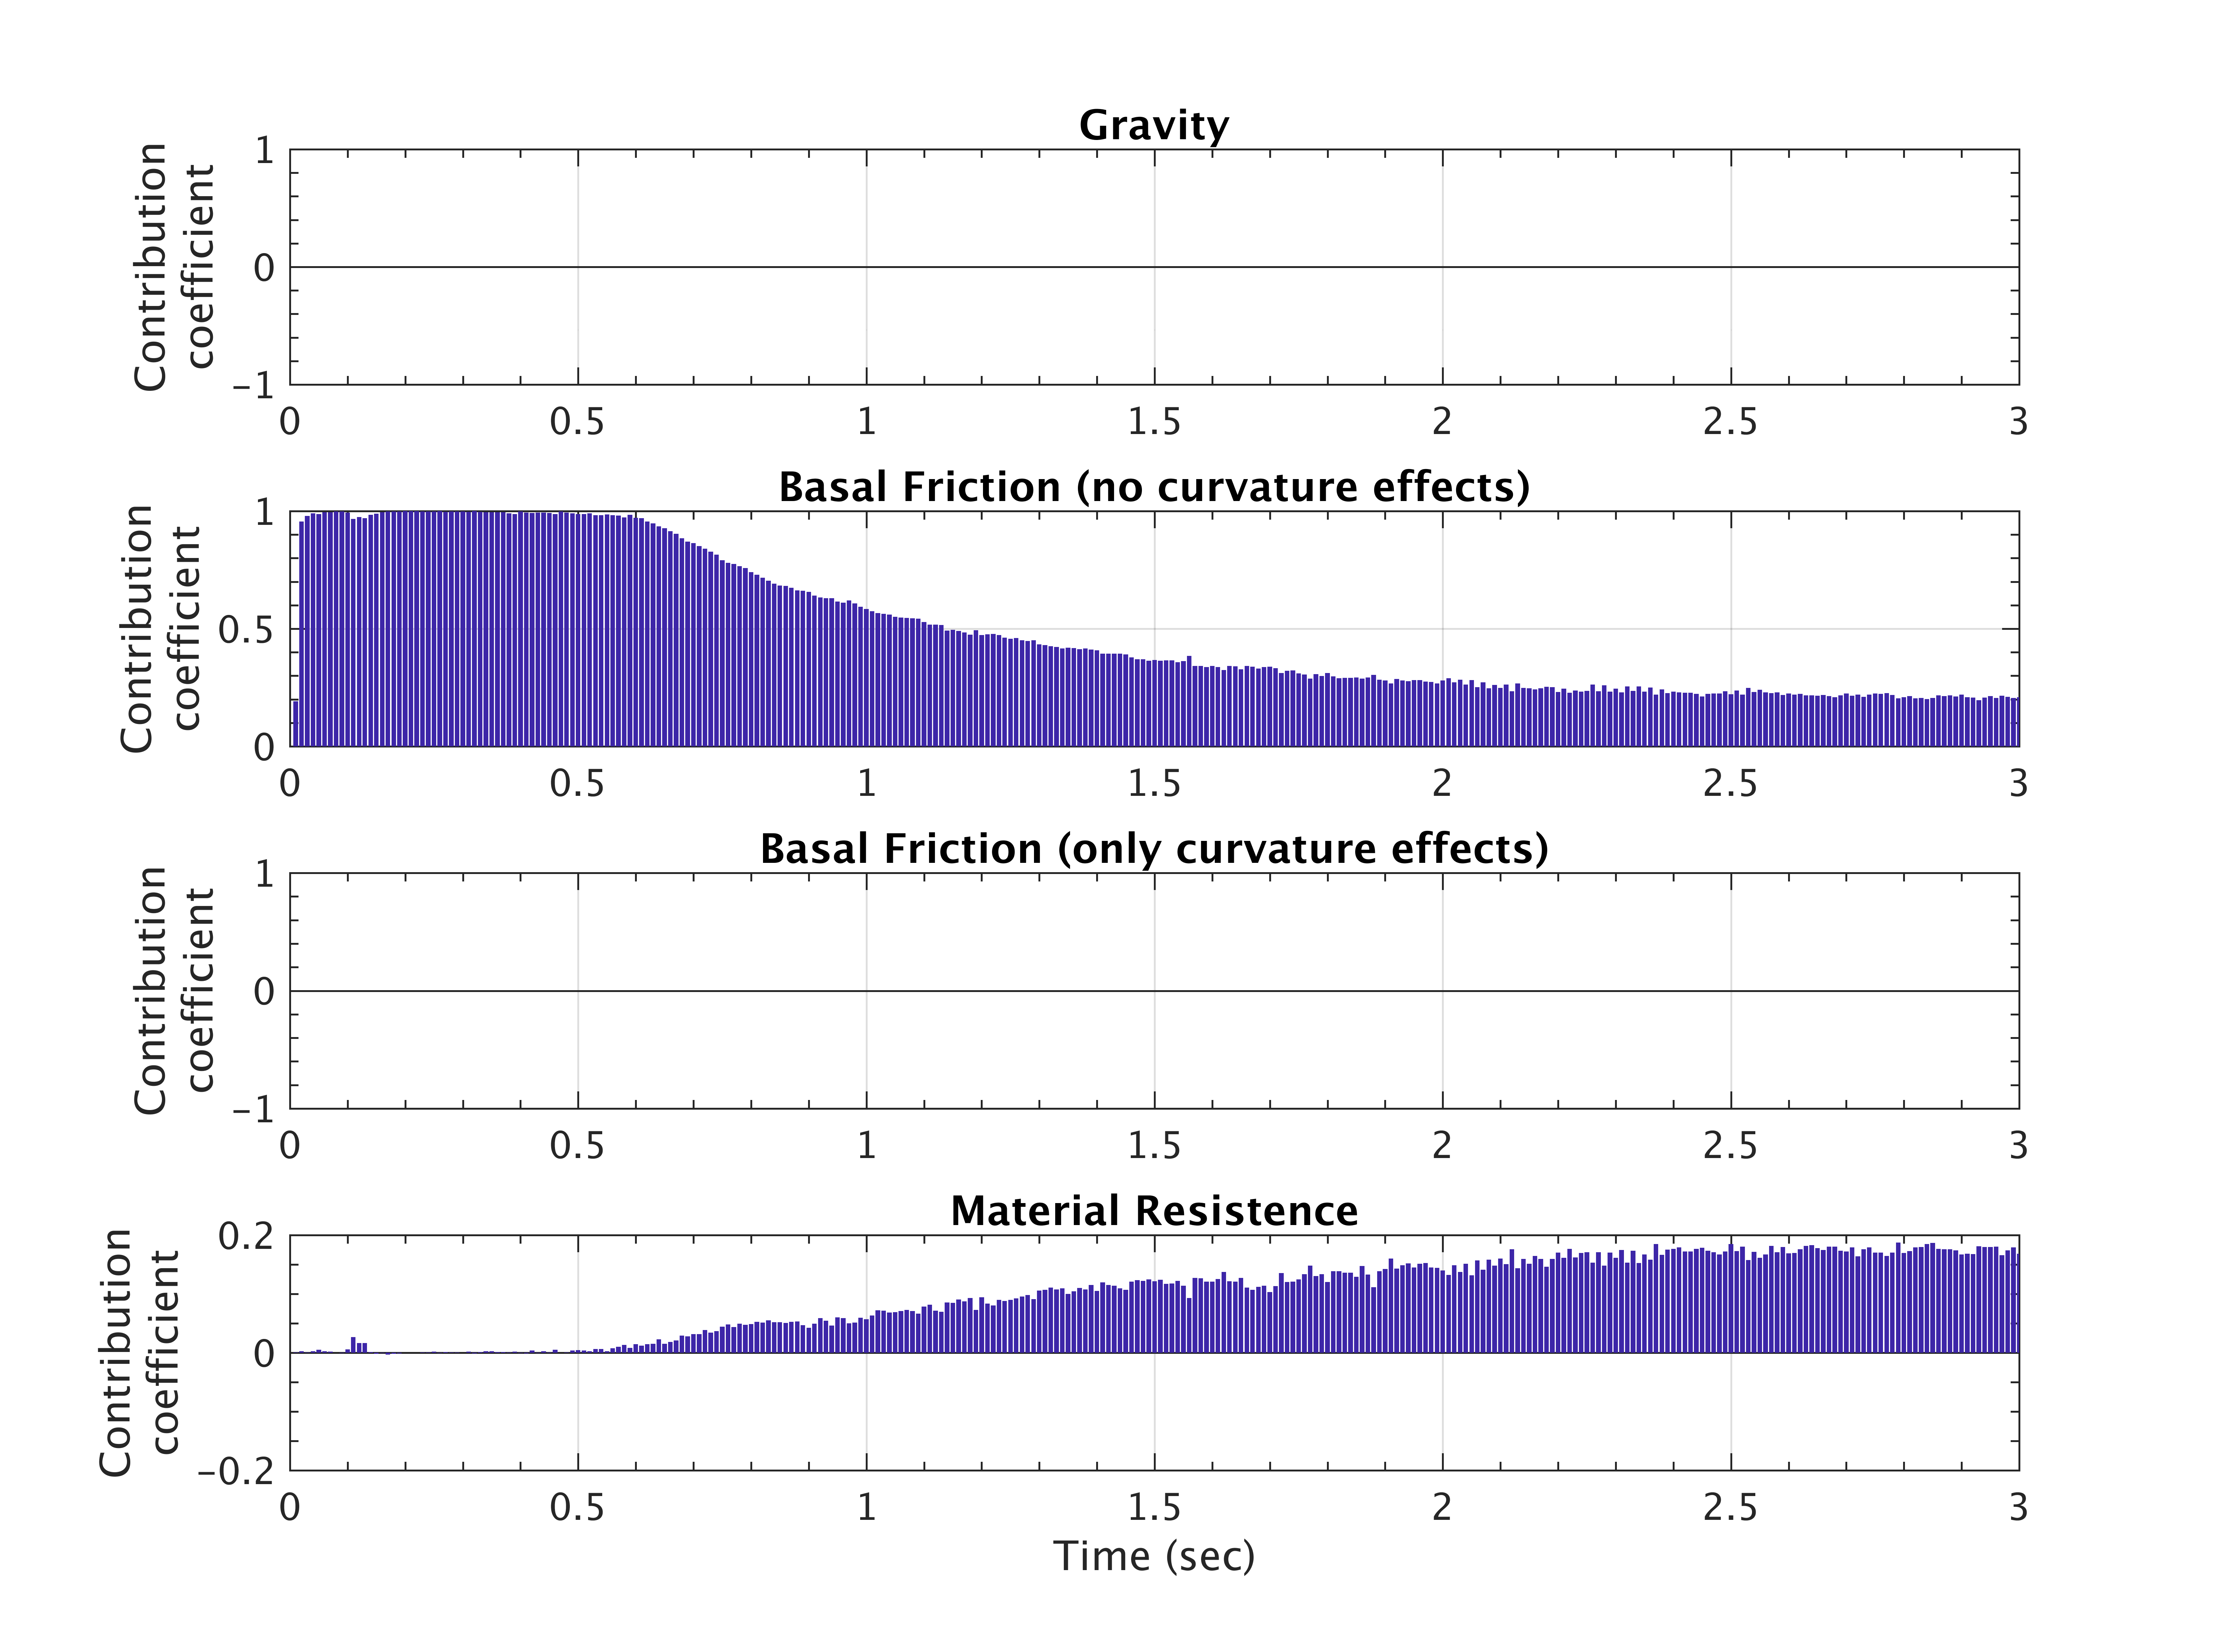
\includegraphics[width=1\textwidth]{InclinedPlane/LocalRecords/ContribF1_P_y.png}
                \subcaption{$x=-0.7, \ y=0.0$, slumping pile location.}
                \label{fig:Ramp-Py1}
        \end{minipage}
        \begin{minipage}[b]{0.5\linewidth}
                \centering
                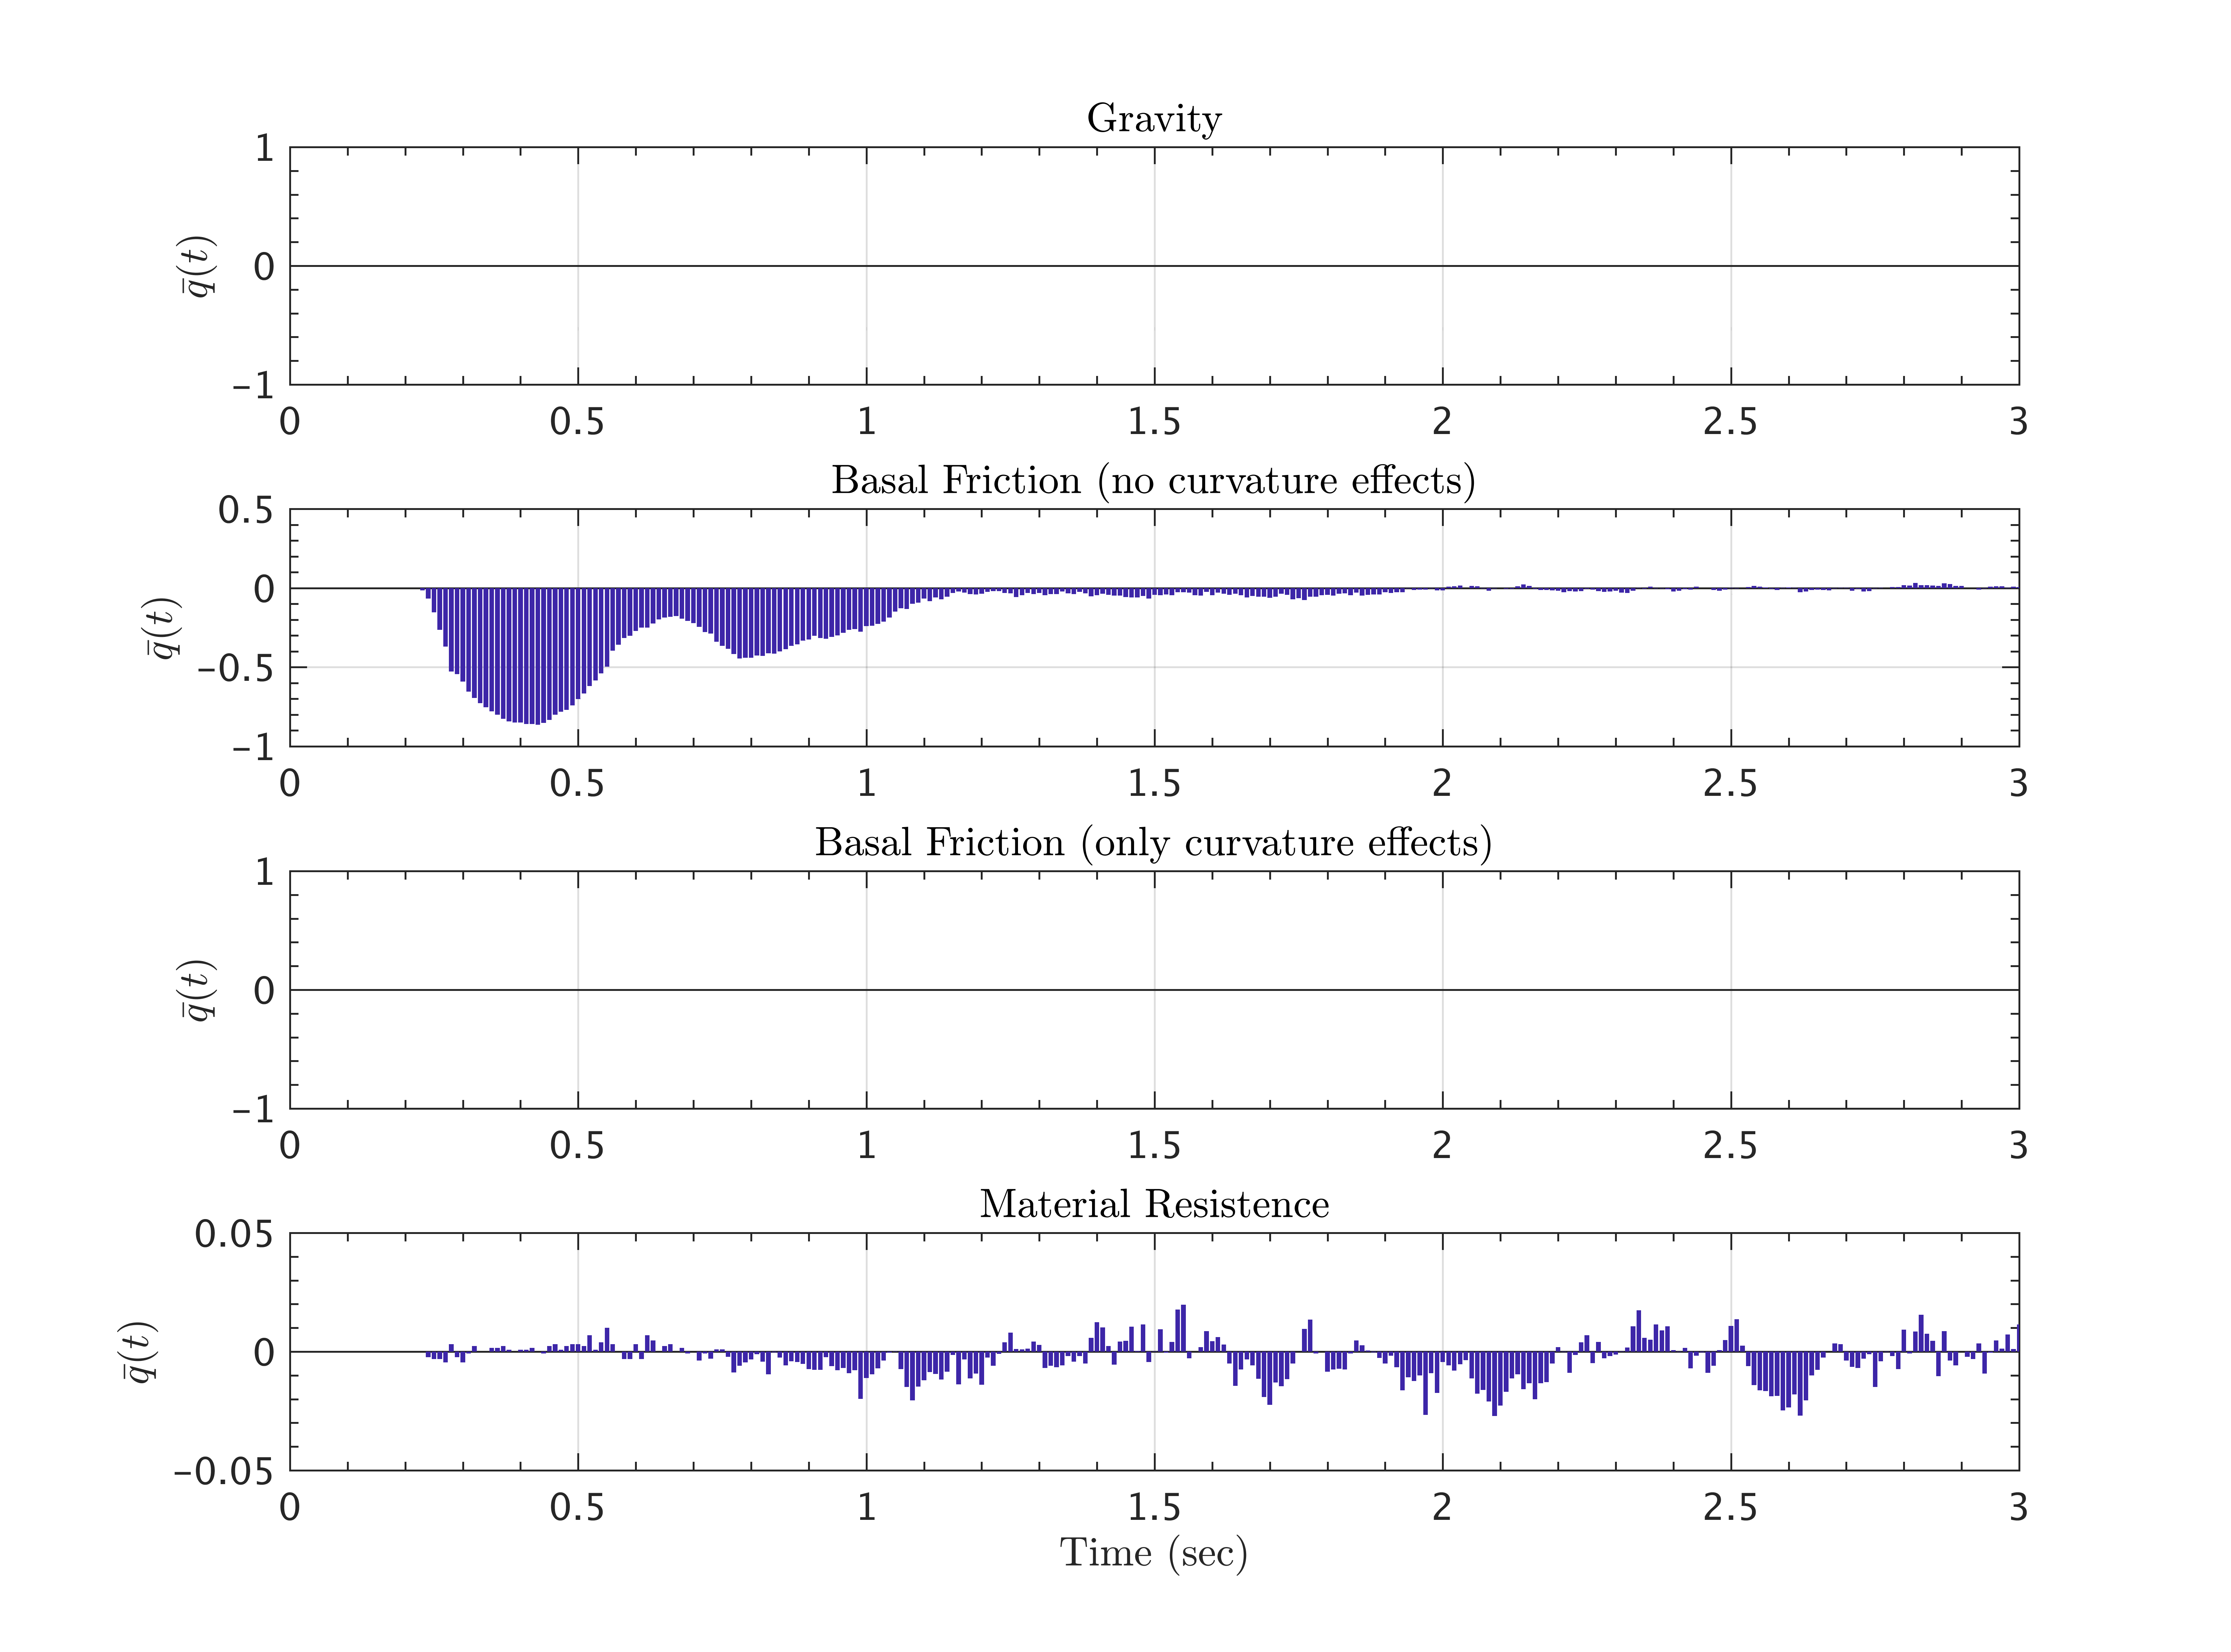
\includegraphics[width=1\textwidth]{InclinedPlane/LocalRecords/ContribF8_P_y.png}
                \subcaption{$x=-0.35, \ y=0.0$, middle point on inclined plane.}
                \label{fig:Ramp-Py2}
        \end{minipage}

        \begin{minipage}[b]{0.5\linewidth}
                \centering
                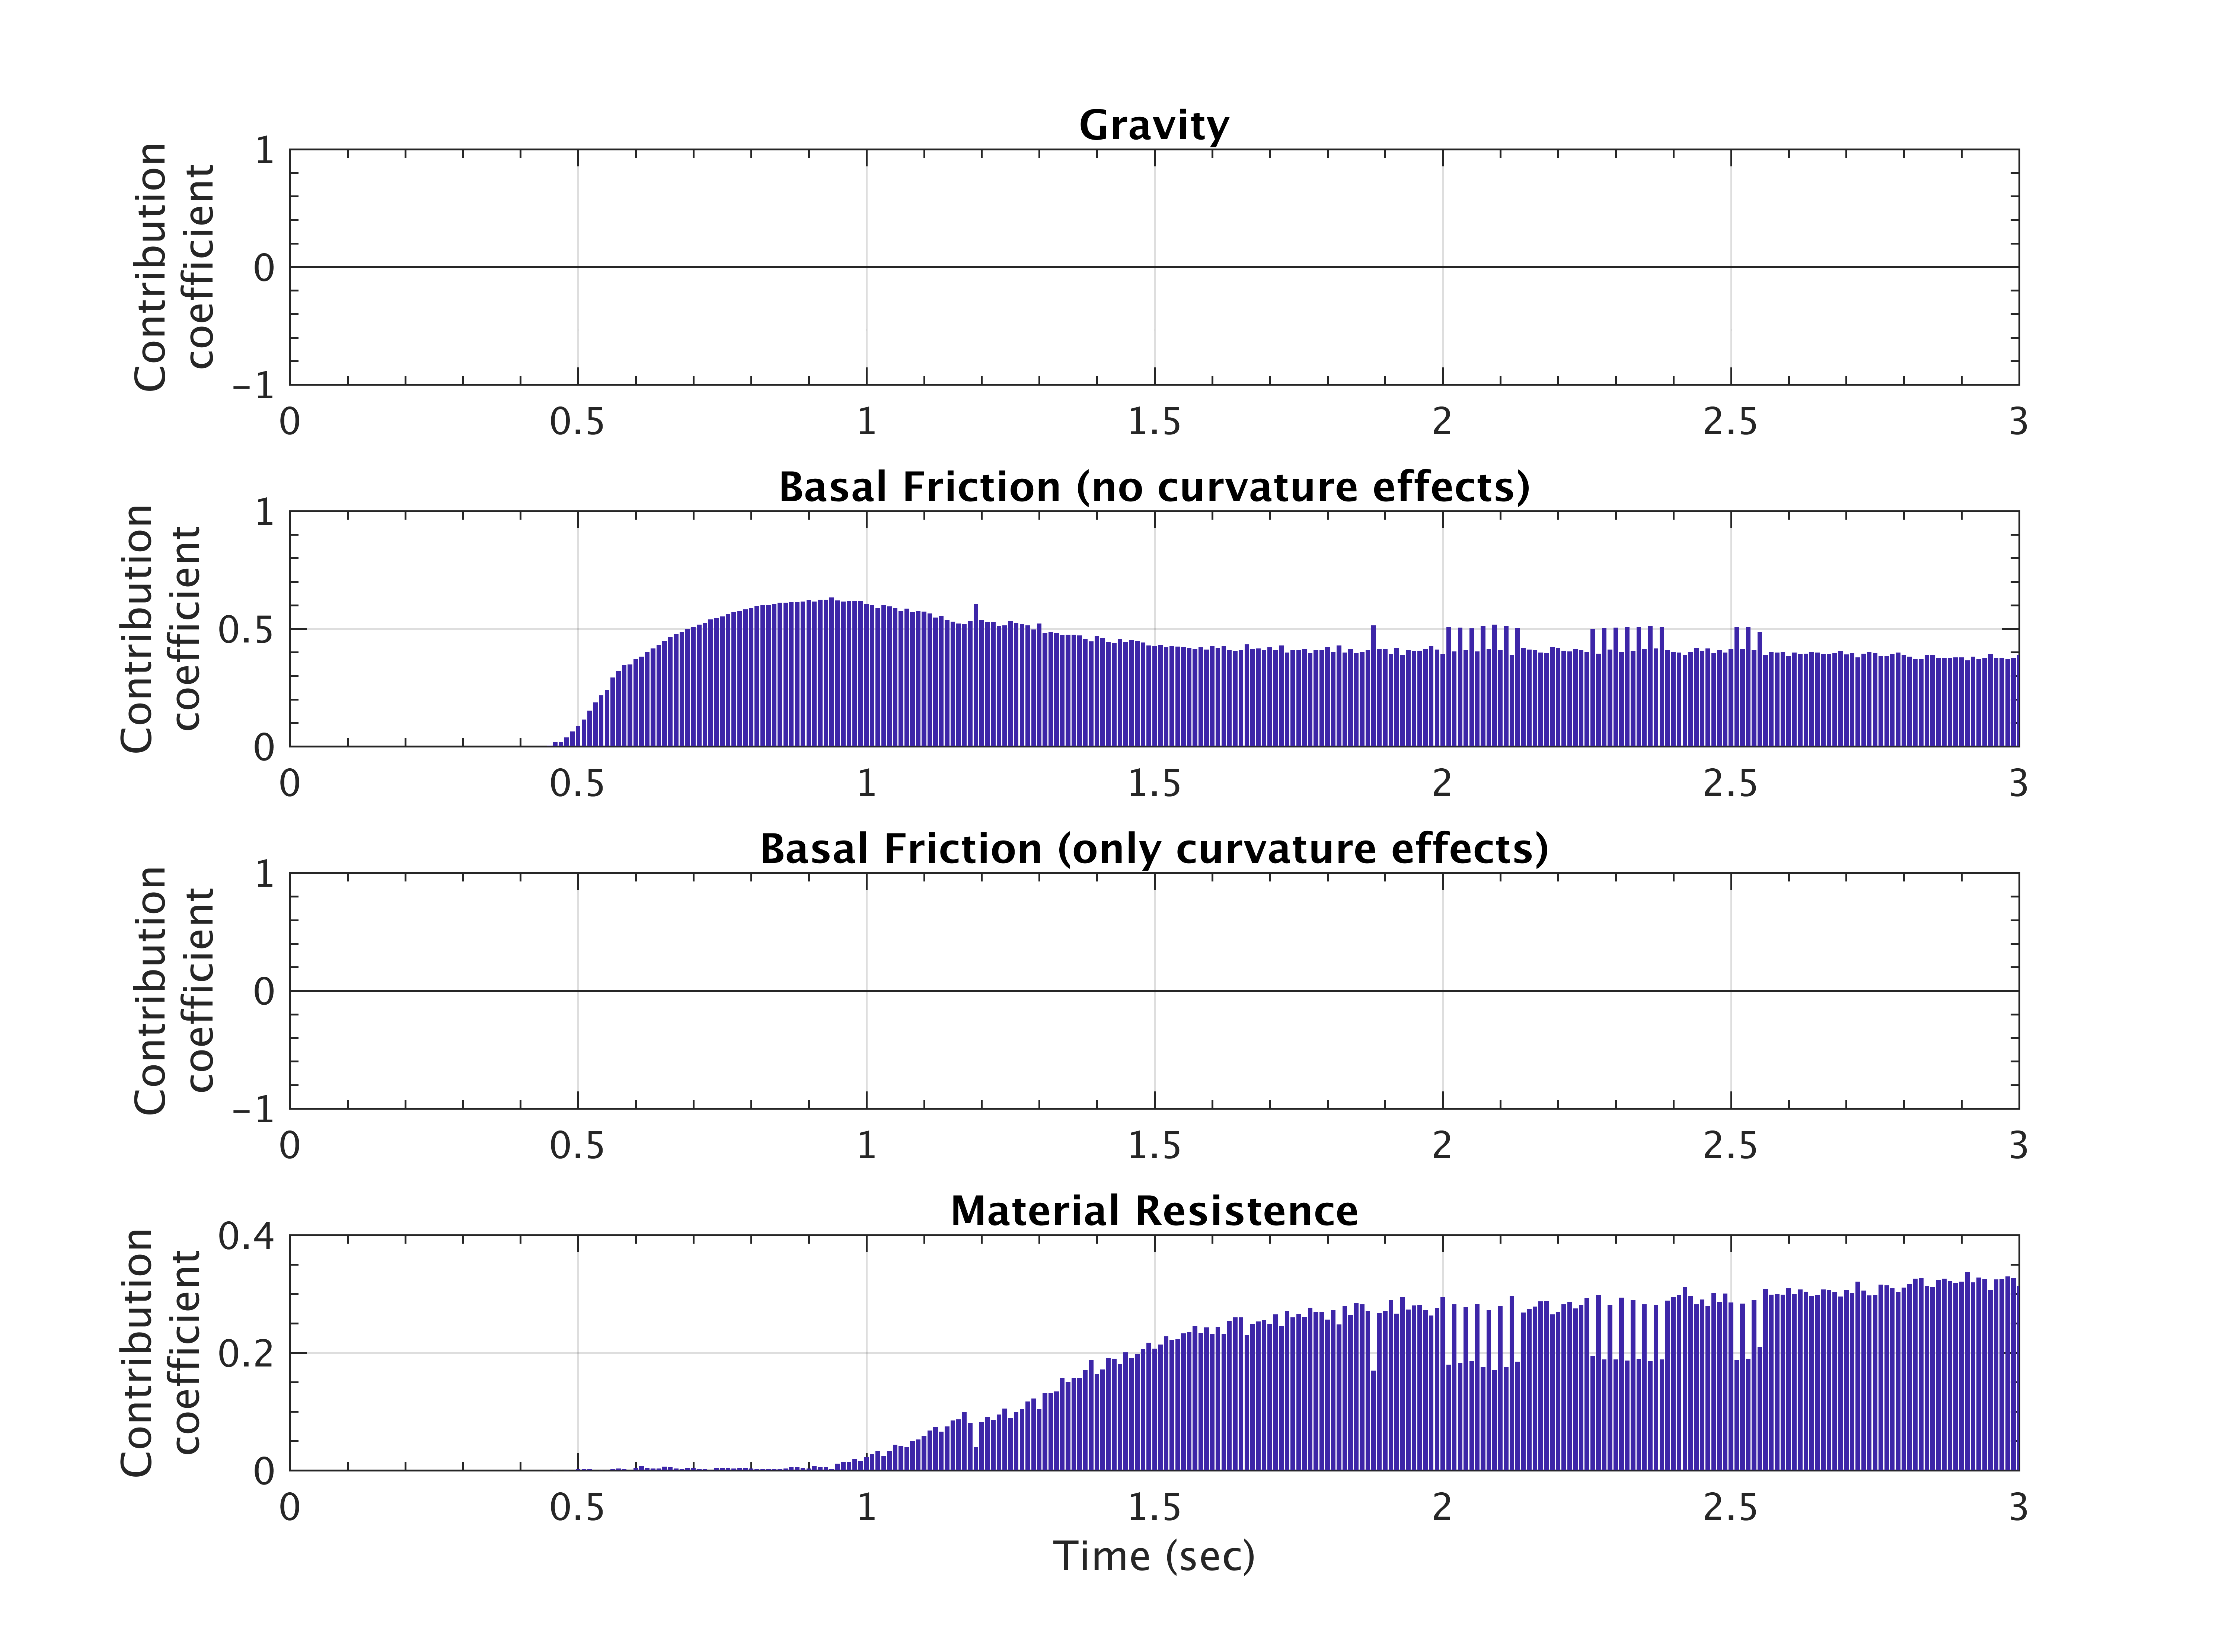
\includegraphics[width=1\textwidth]{InclinedPlane/LocalRecords/ContribF15_P_y.png}
                \subcaption{$x=0, \ y=0$, inclined and runout planes' joint location.}
                \label{fig:Ramp-Py3}
        \end{minipage}
        \begin{minipage}[b]{0.5\linewidth}
                \centering
                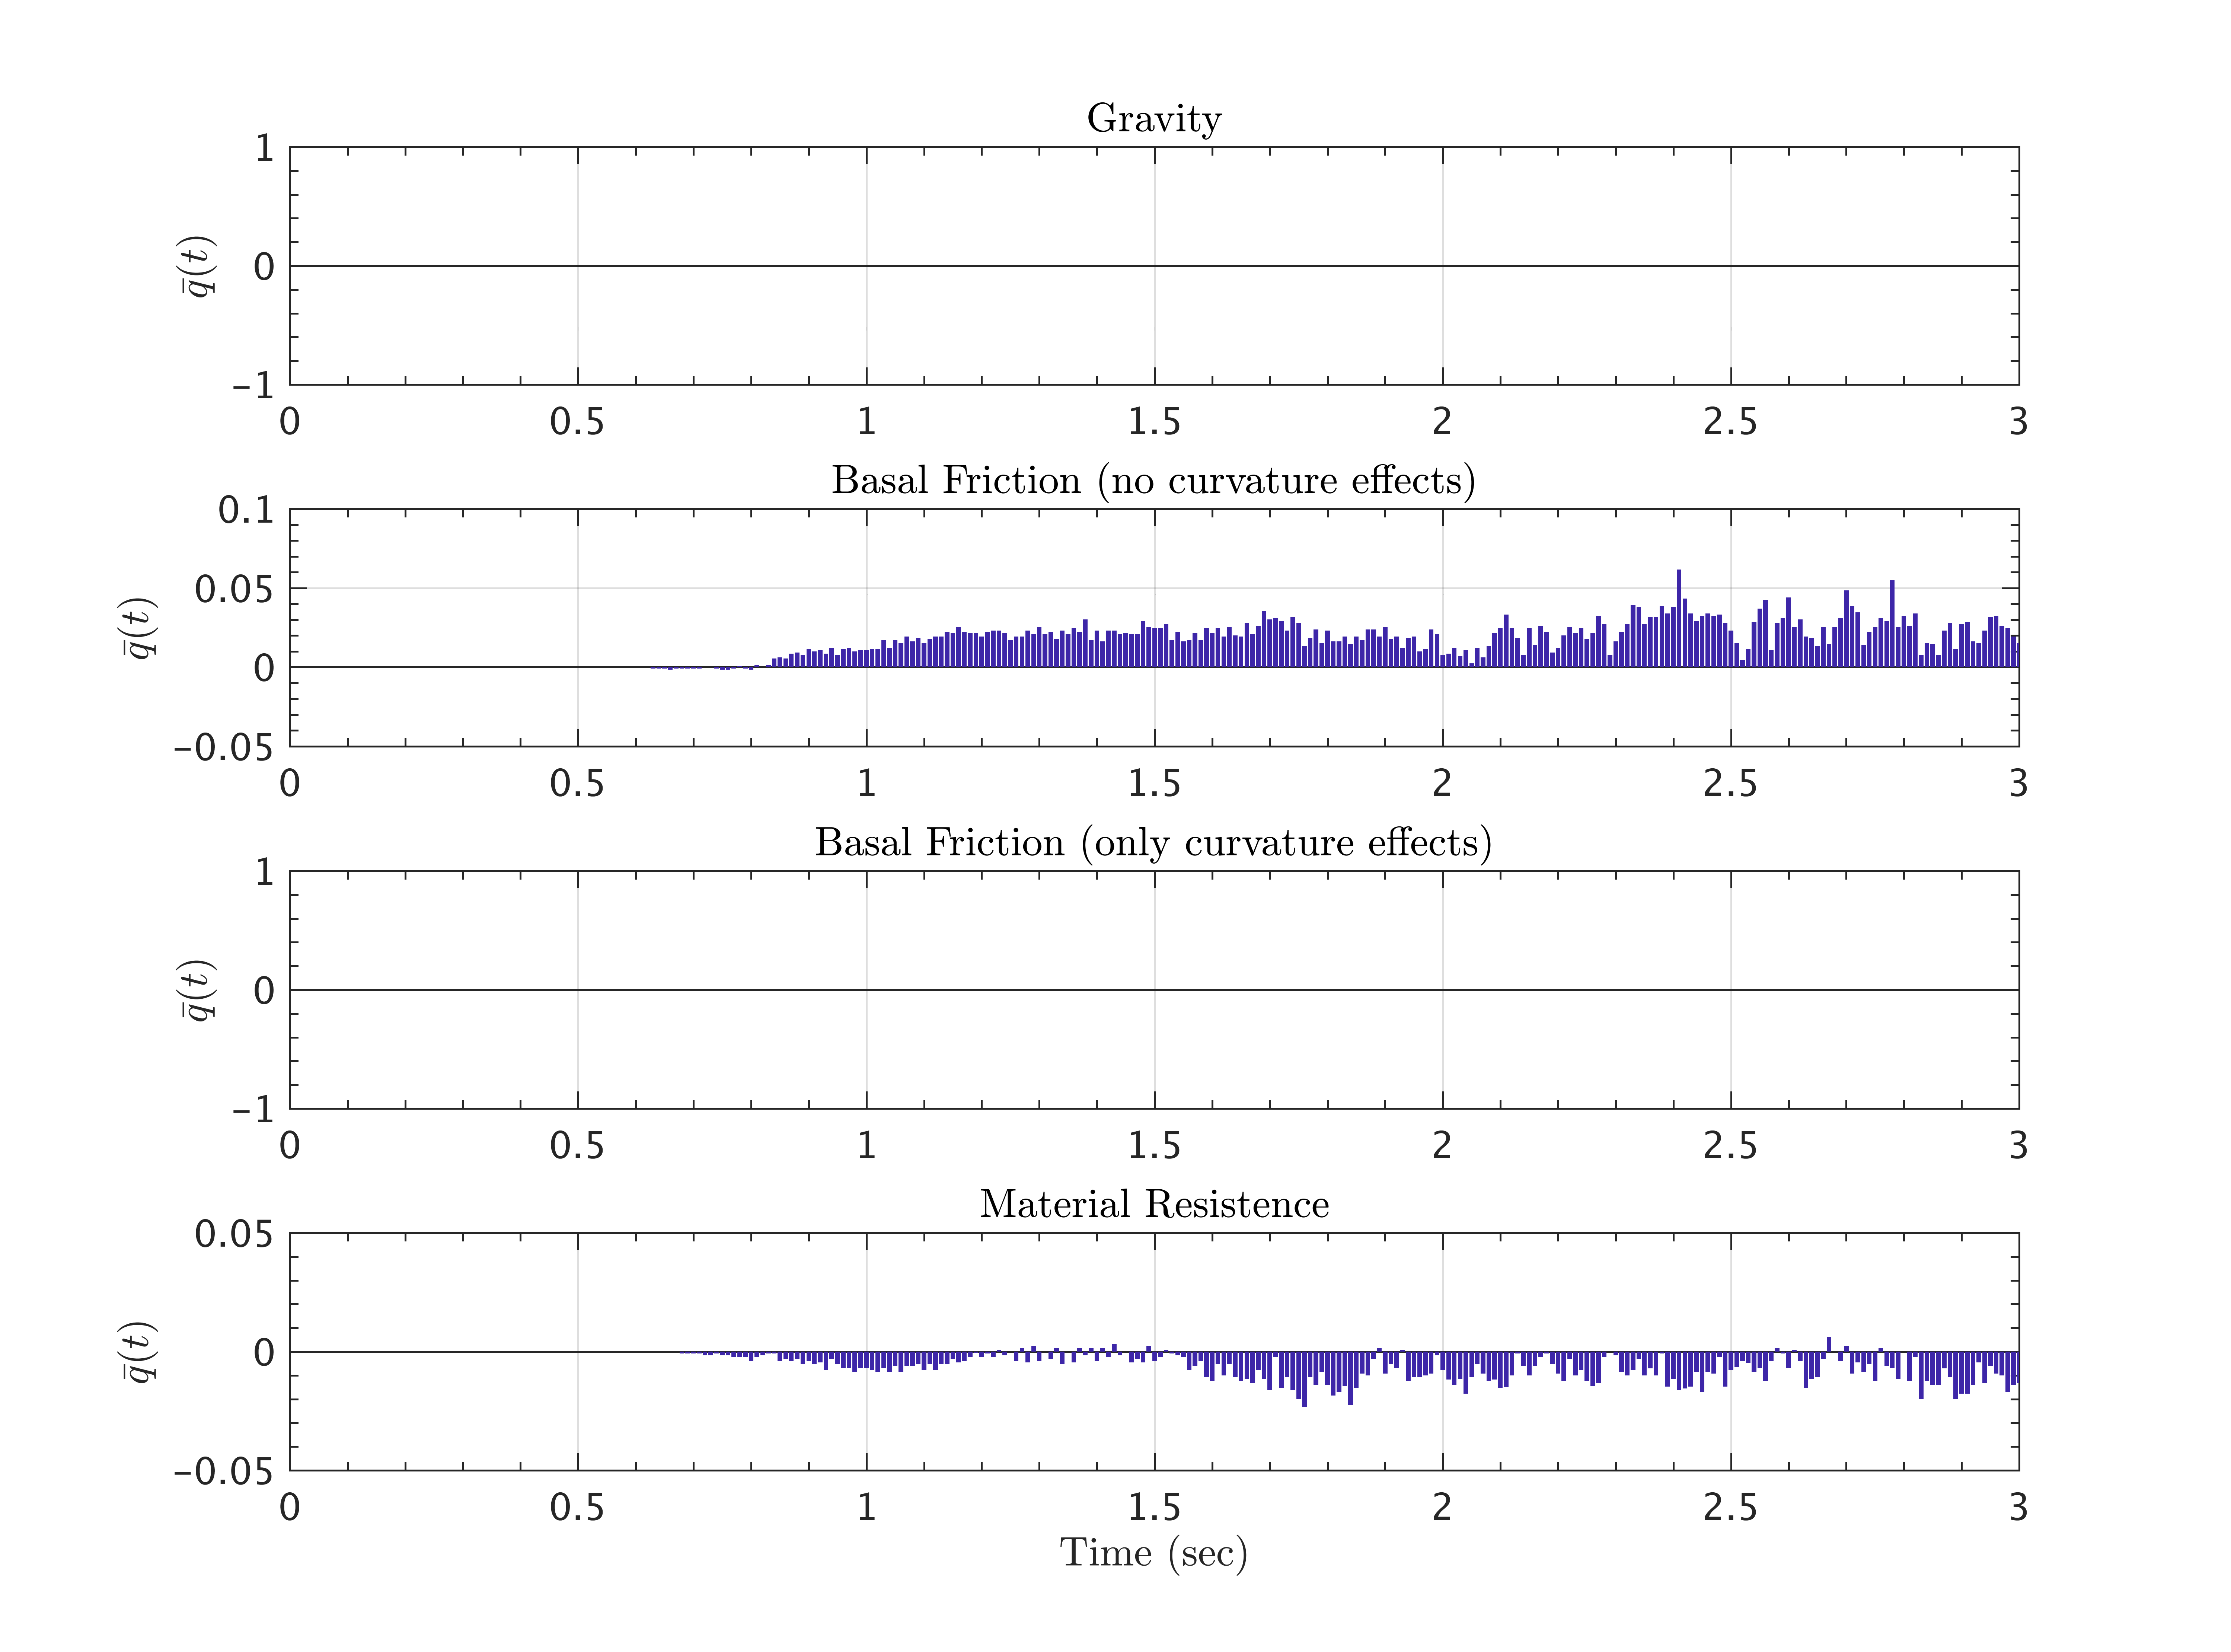
\includegraphics[width=1\textwidth]{InclinedPlane/LocalRecords/ContribF17_P_y.png}
                \subcaption{$x=0.15, \ y=0.0$, a location on runout plane.}
                \label{fig:Ramp-Py4}
        \end{minipage}
        \caption{Time history of mean values for force impact quotients, $\bar{q}_i(t)$, along the lateral direction, Pouliquen-Forterre model.}
        \label{fig:Ramp-Py}
\end{figure}


\subsubsection{Voellmy-Salm Model, Force Impact Quotients}
\begin{figure}[H]
        \begin{minipage}[b]{0.5\linewidth}
                \centering
                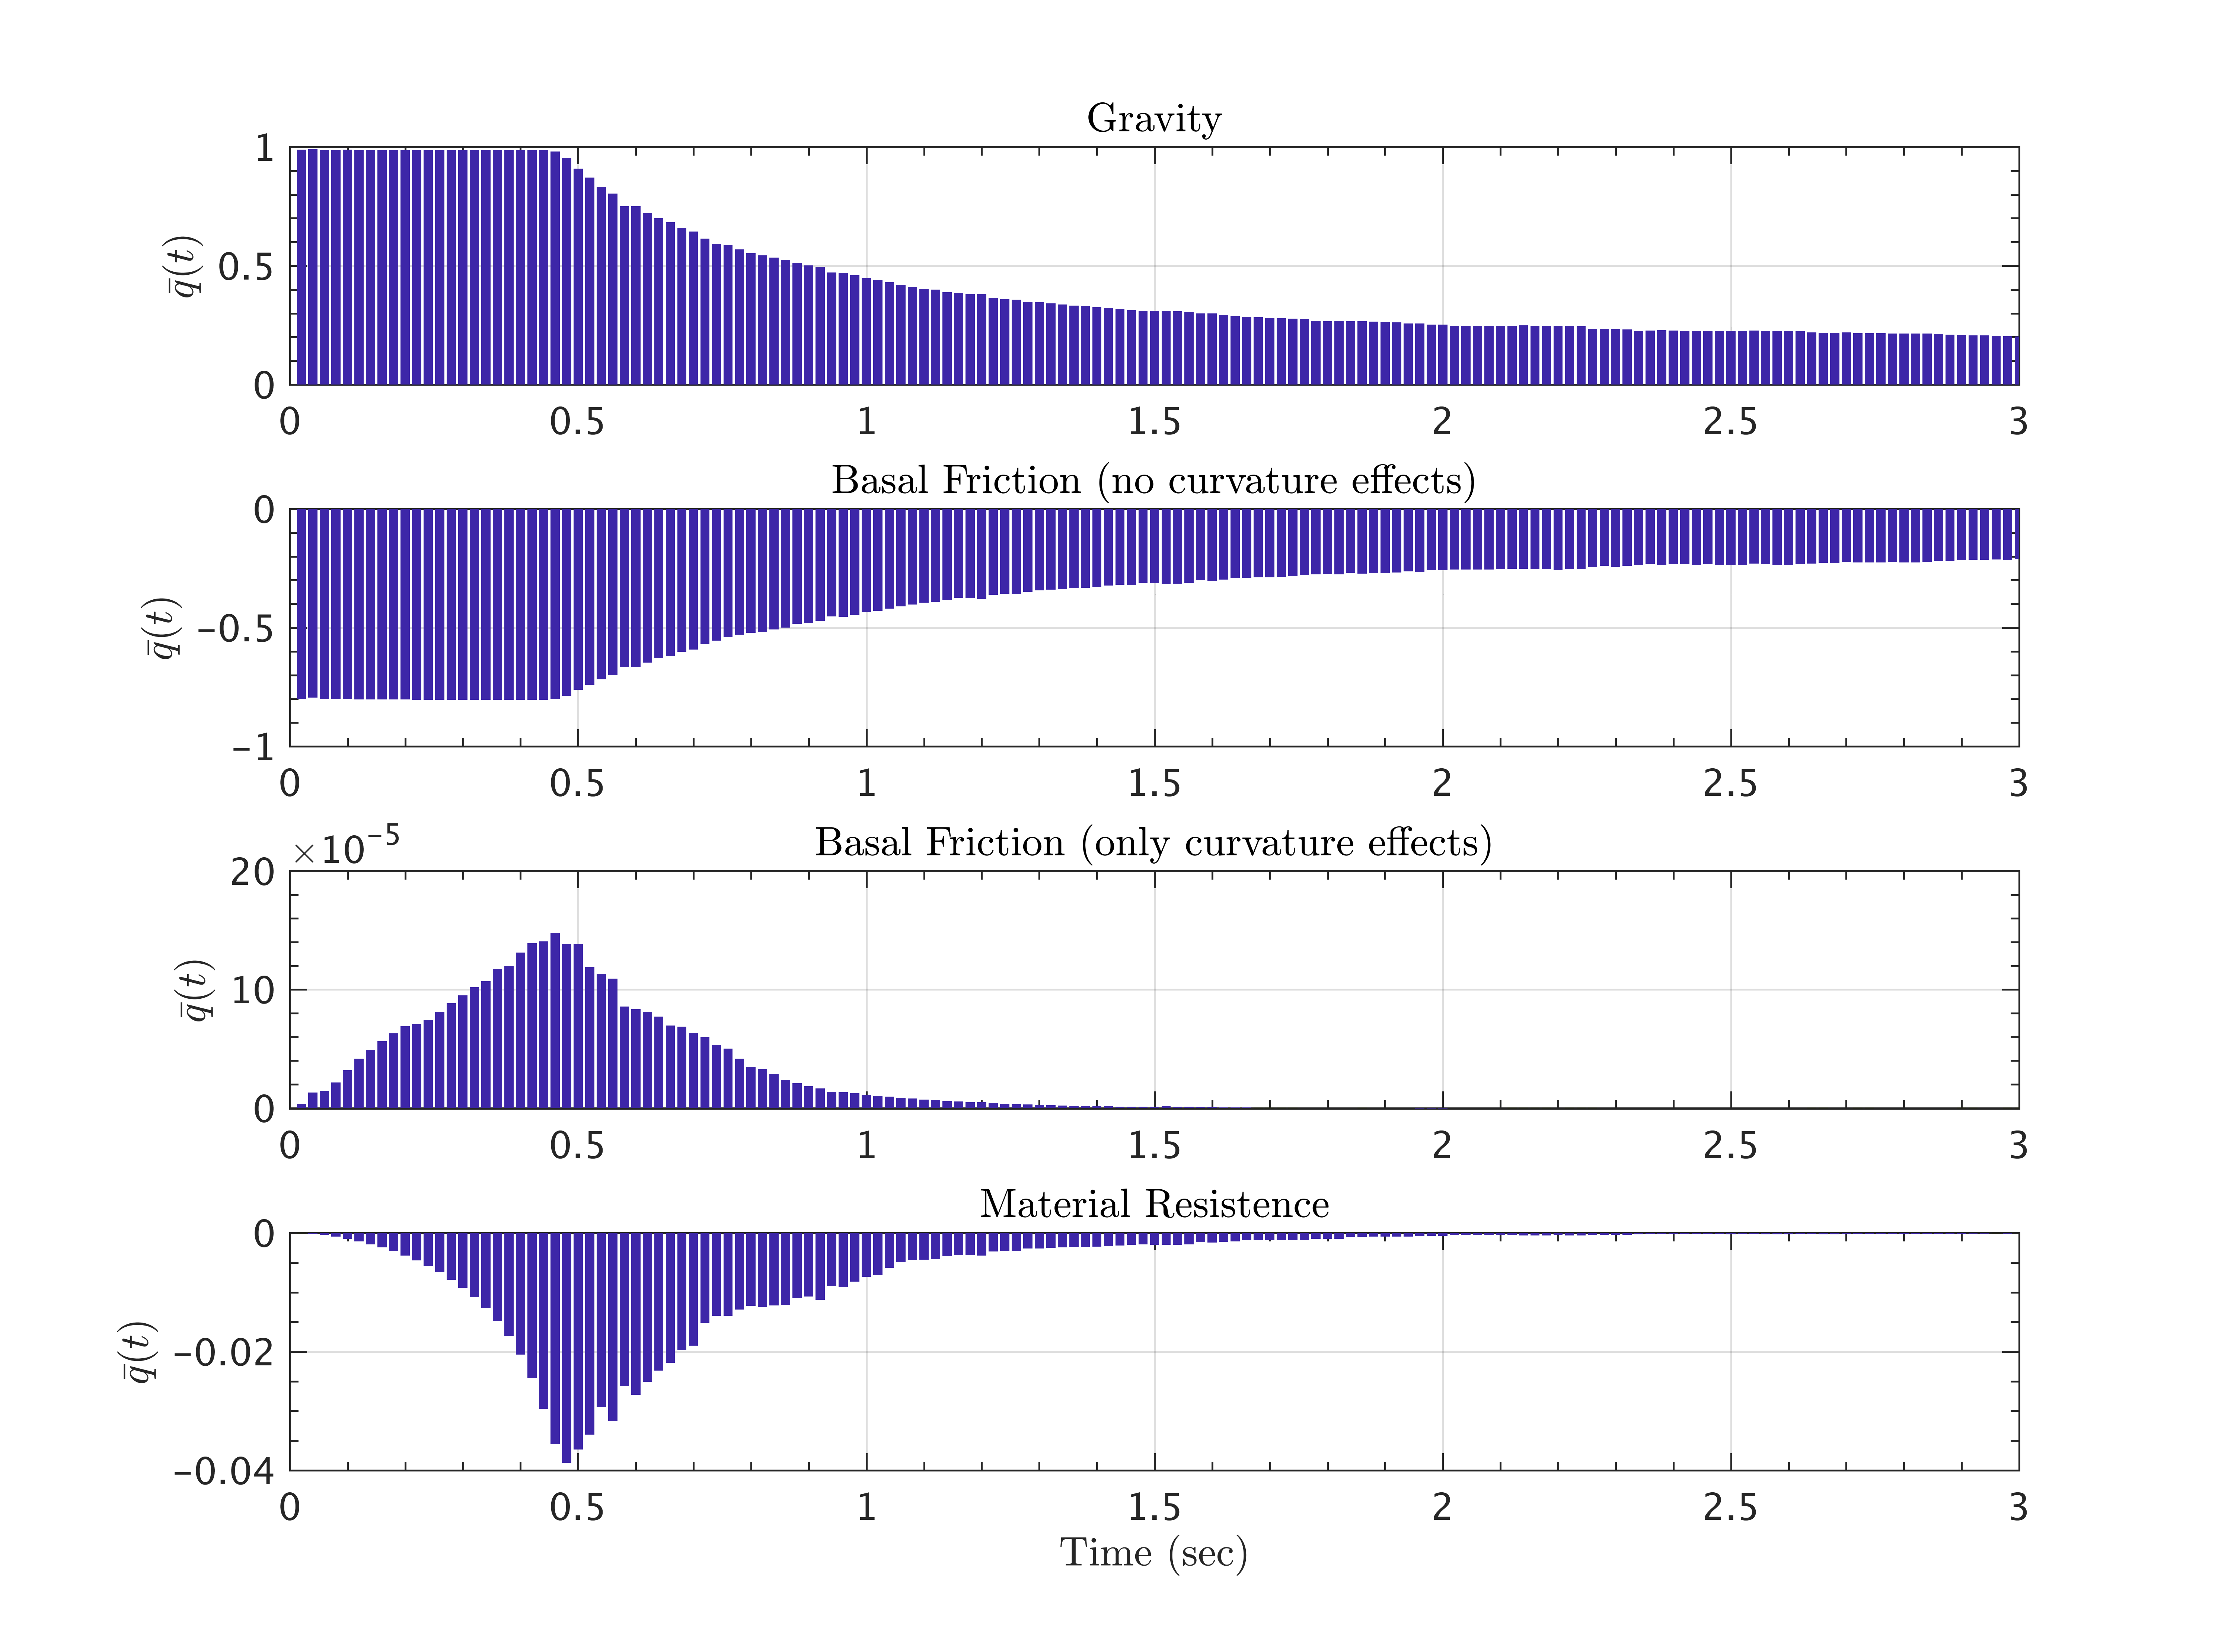
\includegraphics[width=1\textwidth]{InclinedPlane/LocalRecords/ContribF1_V_x.png}
                \subcaption{$x=-0.7, \ y=0.0$, slumping pile location.}
                \label{fig:Ramp-Vx1}
        \end{minipage}
        \begin{minipage}[b]{0.5\linewidth}
                \centering
                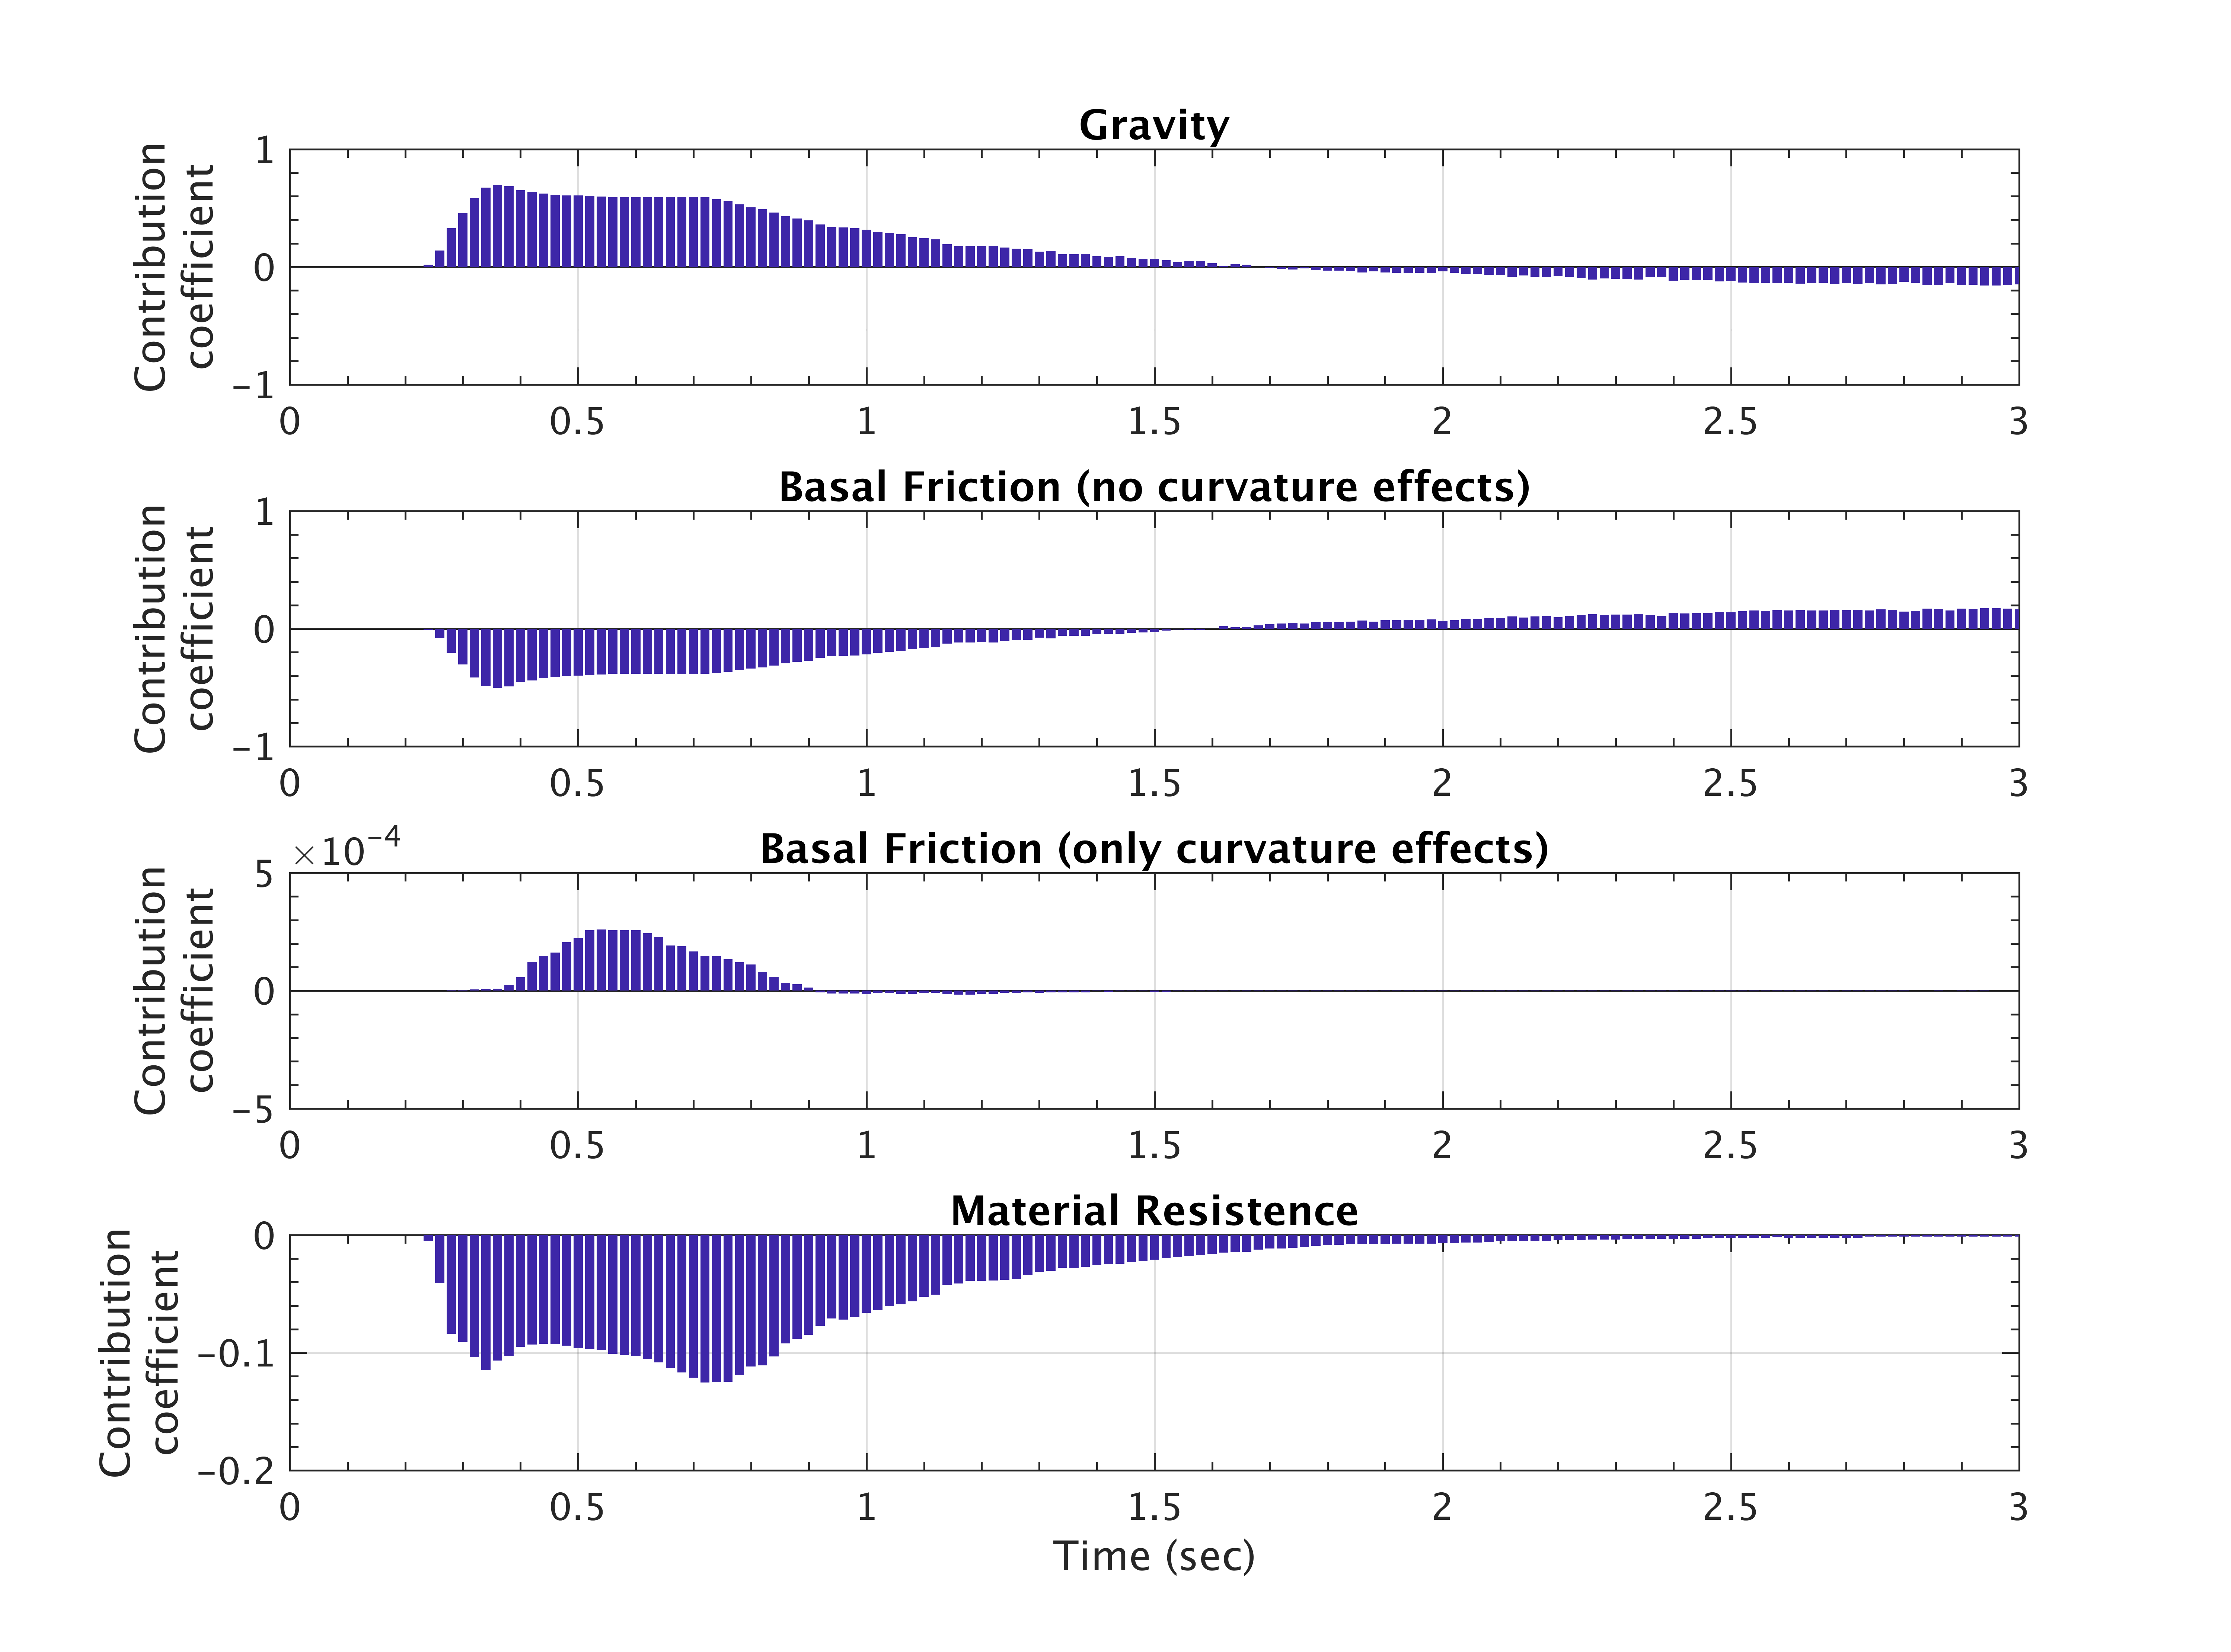
\includegraphics[width=1\textwidth]{InclinedPlane/LocalRecords/ContribF8_V_x.png}
                \subcaption{$x=-0.35, \ y=0.0$, middle point on inclined plane.}
                \label{fig:Ramp-Vx2}
        \end{minipage}

        \begin{minipage}[b]{0.5\linewidth}
                \centering
                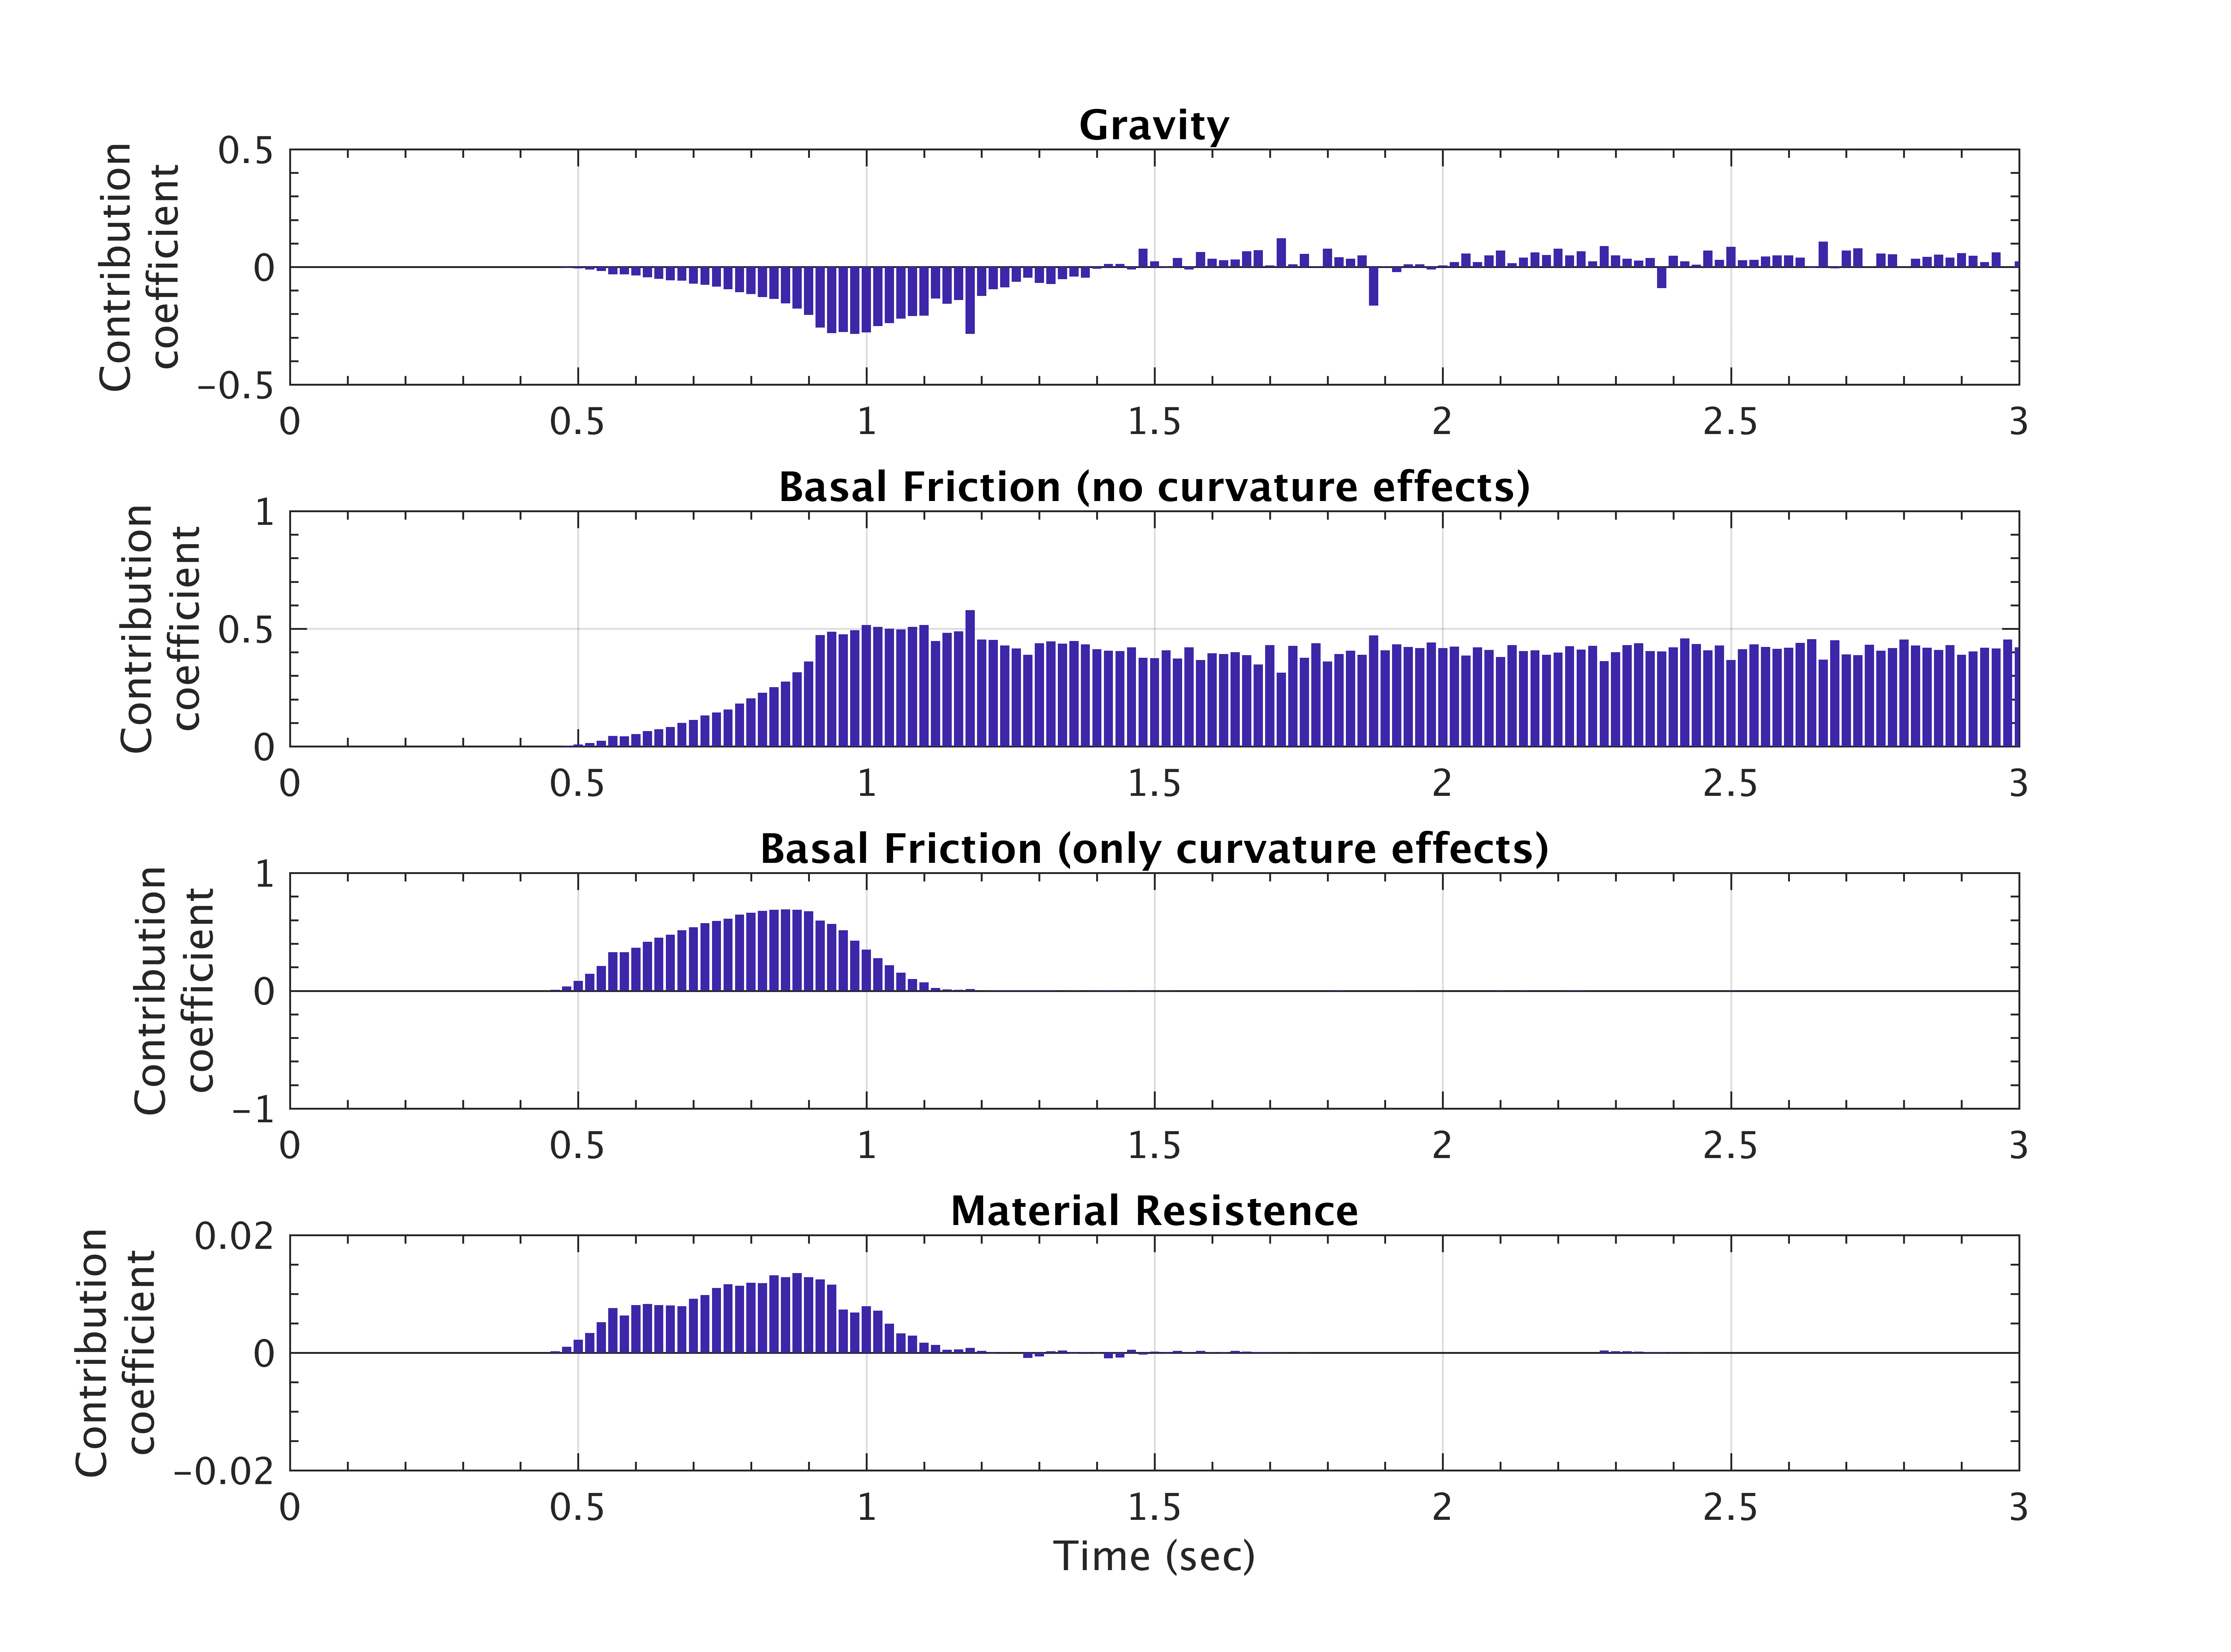
\includegraphics[width=1\textwidth]{InclinedPlane/LocalRecords/ContribF15_V_x.png}
                \subcaption{$x=0, \ y=0$, inclined and runout planes' joint location.}
                \label{fig:Ramp-Vx3}
        \end{minipage}
        \begin{minipage}[b]{0.5\linewidth}
                \centering
                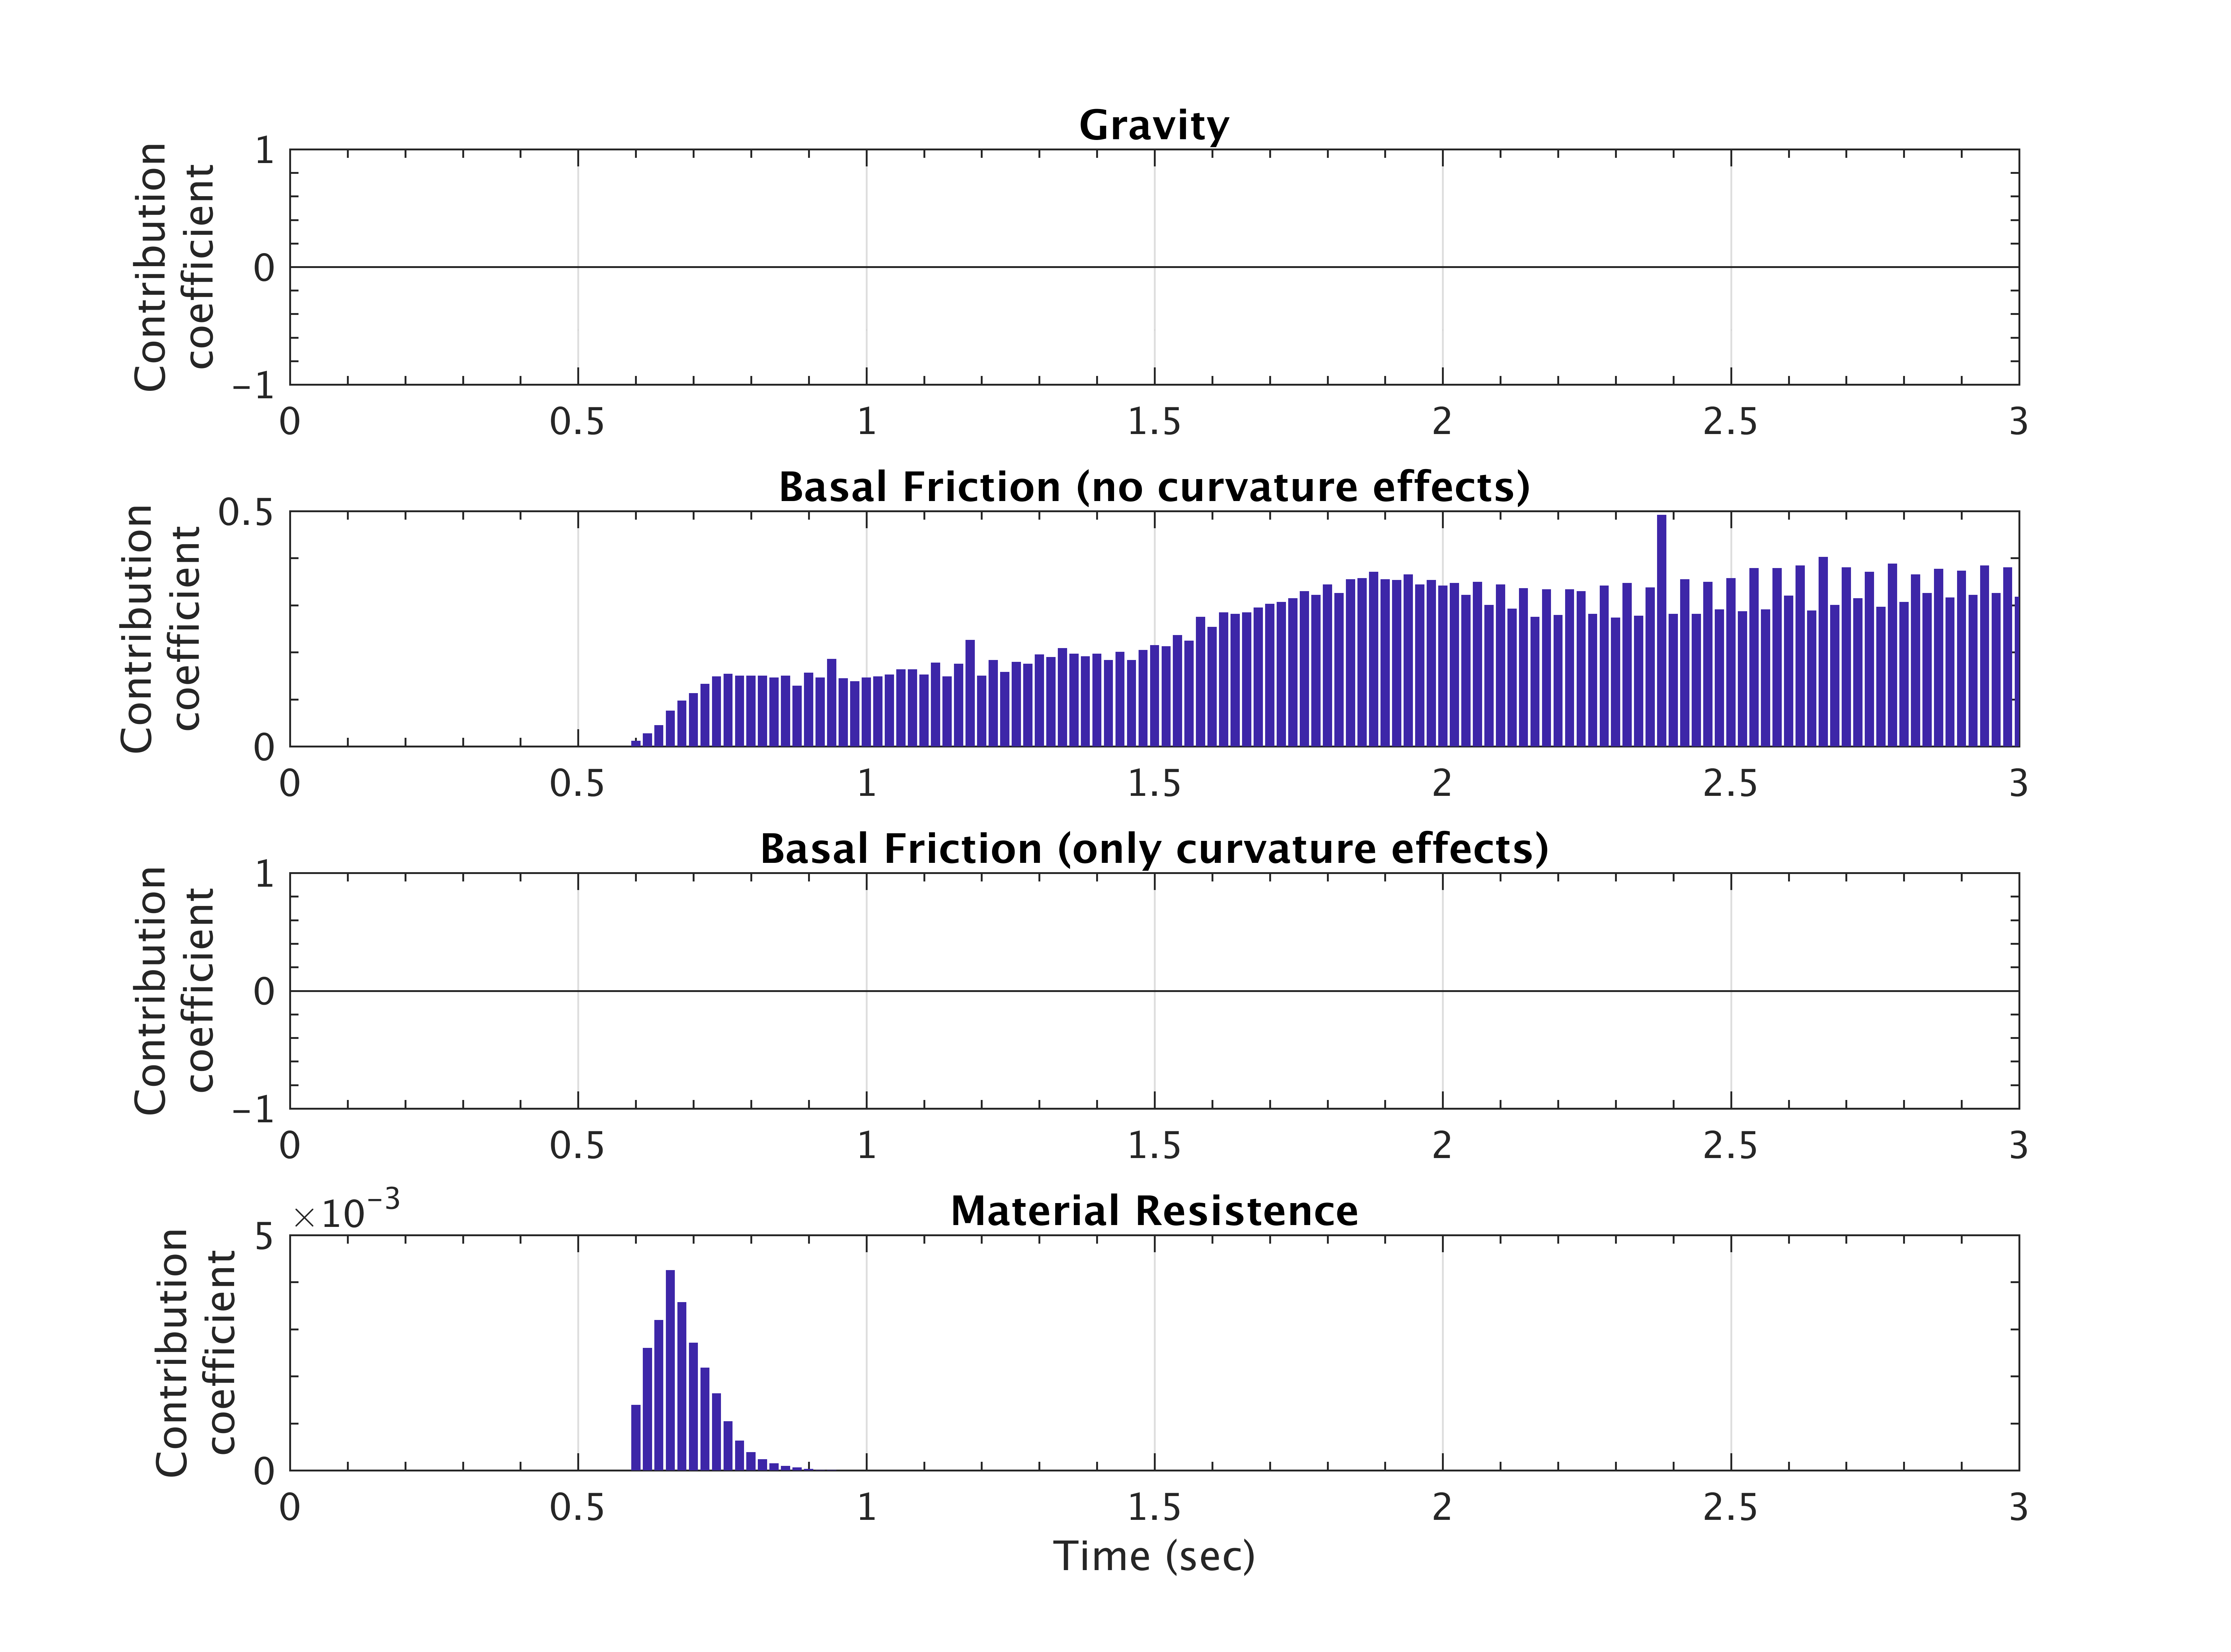
\includegraphics[width=1\textwidth]{InclinedPlane/LocalRecords/ContribF17_V_x.png}
                \subcaption{$x=0.15, \ y=0.0$, a location on runout plane.}
                \label{fig:Ramp-Vx4}
        \end{minipage}
        \caption{Time history of mean values for force impact quotients, $\bar{q}_i(t)$, along runout direction, Voellmy-Salm model.}
        \label{fig:Ramp-Vx}
\end{figure}

\begin{figure}[H]
        \begin{minipage}[b]{0.5\linewidth}
                \centering
                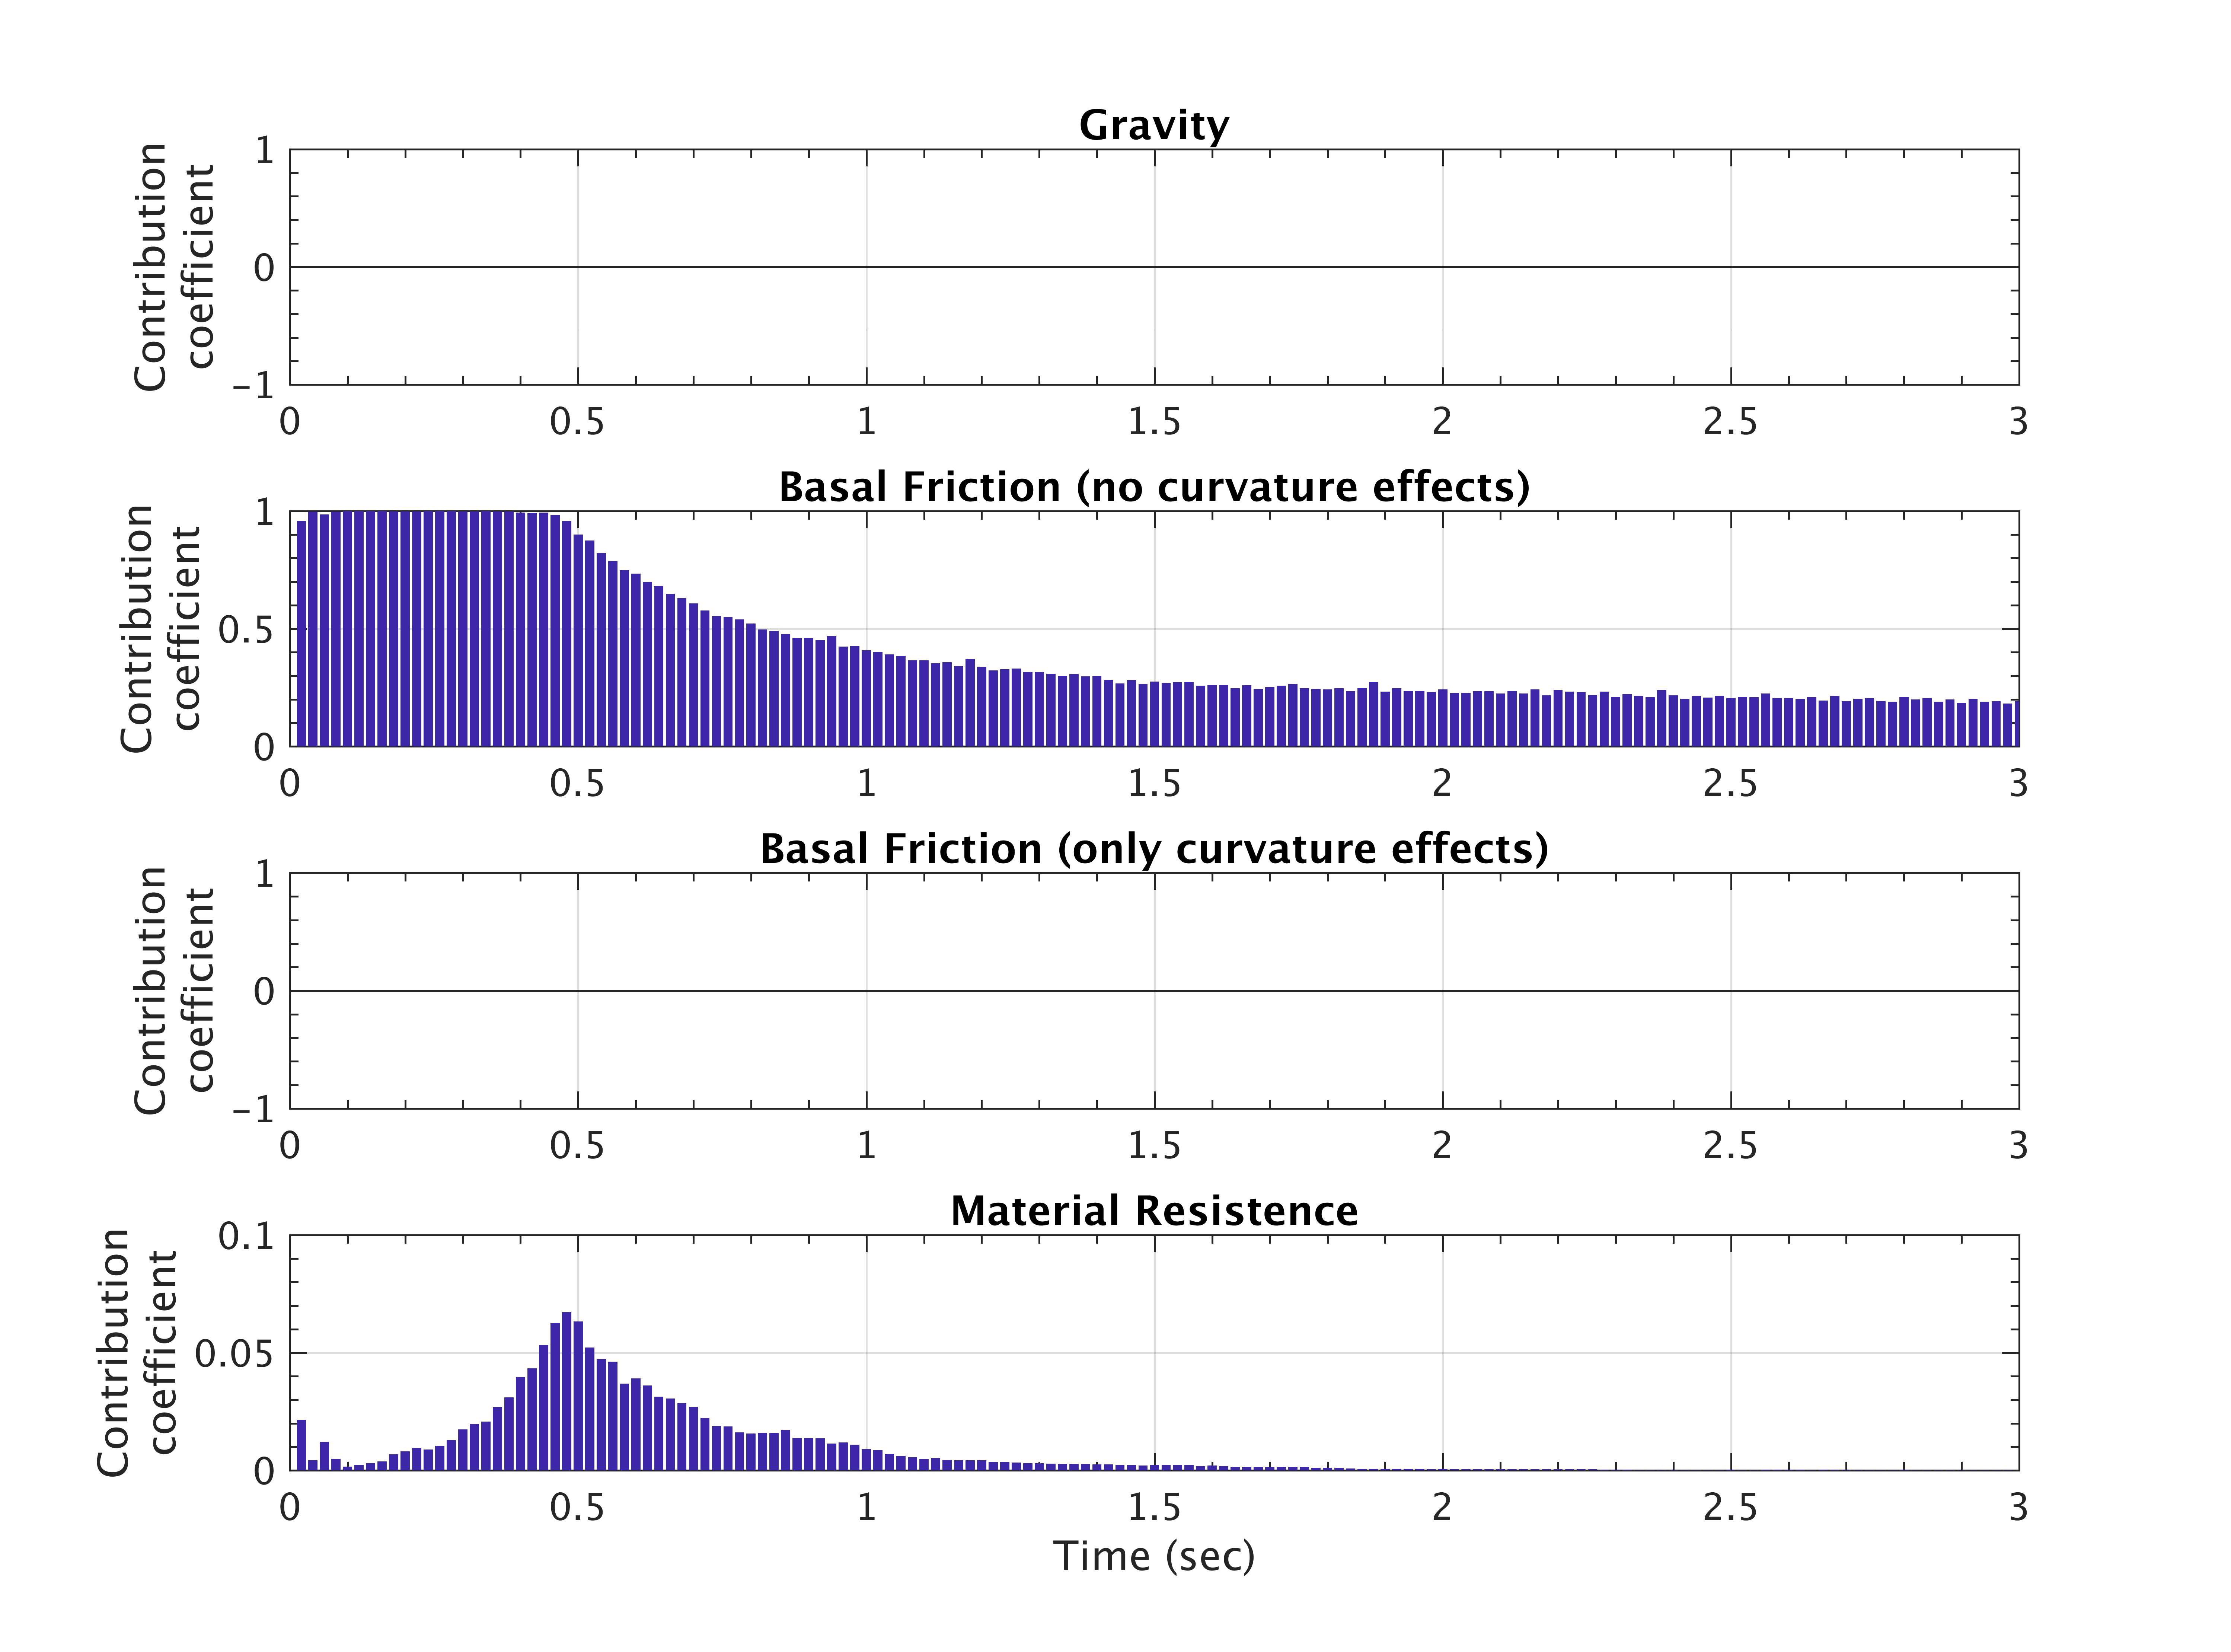
\includegraphics[width=1\textwidth]{InclinedPlane/LocalRecords/ContribF1_V_y.png}
                \subcaption{$x=-0.7, \ y=0.0$, slumping pile location.}
                \label{fig:Ramp-Vy1}
        \end{minipage}
        \begin{minipage}[b]{0.5\linewidth}
                \centering
                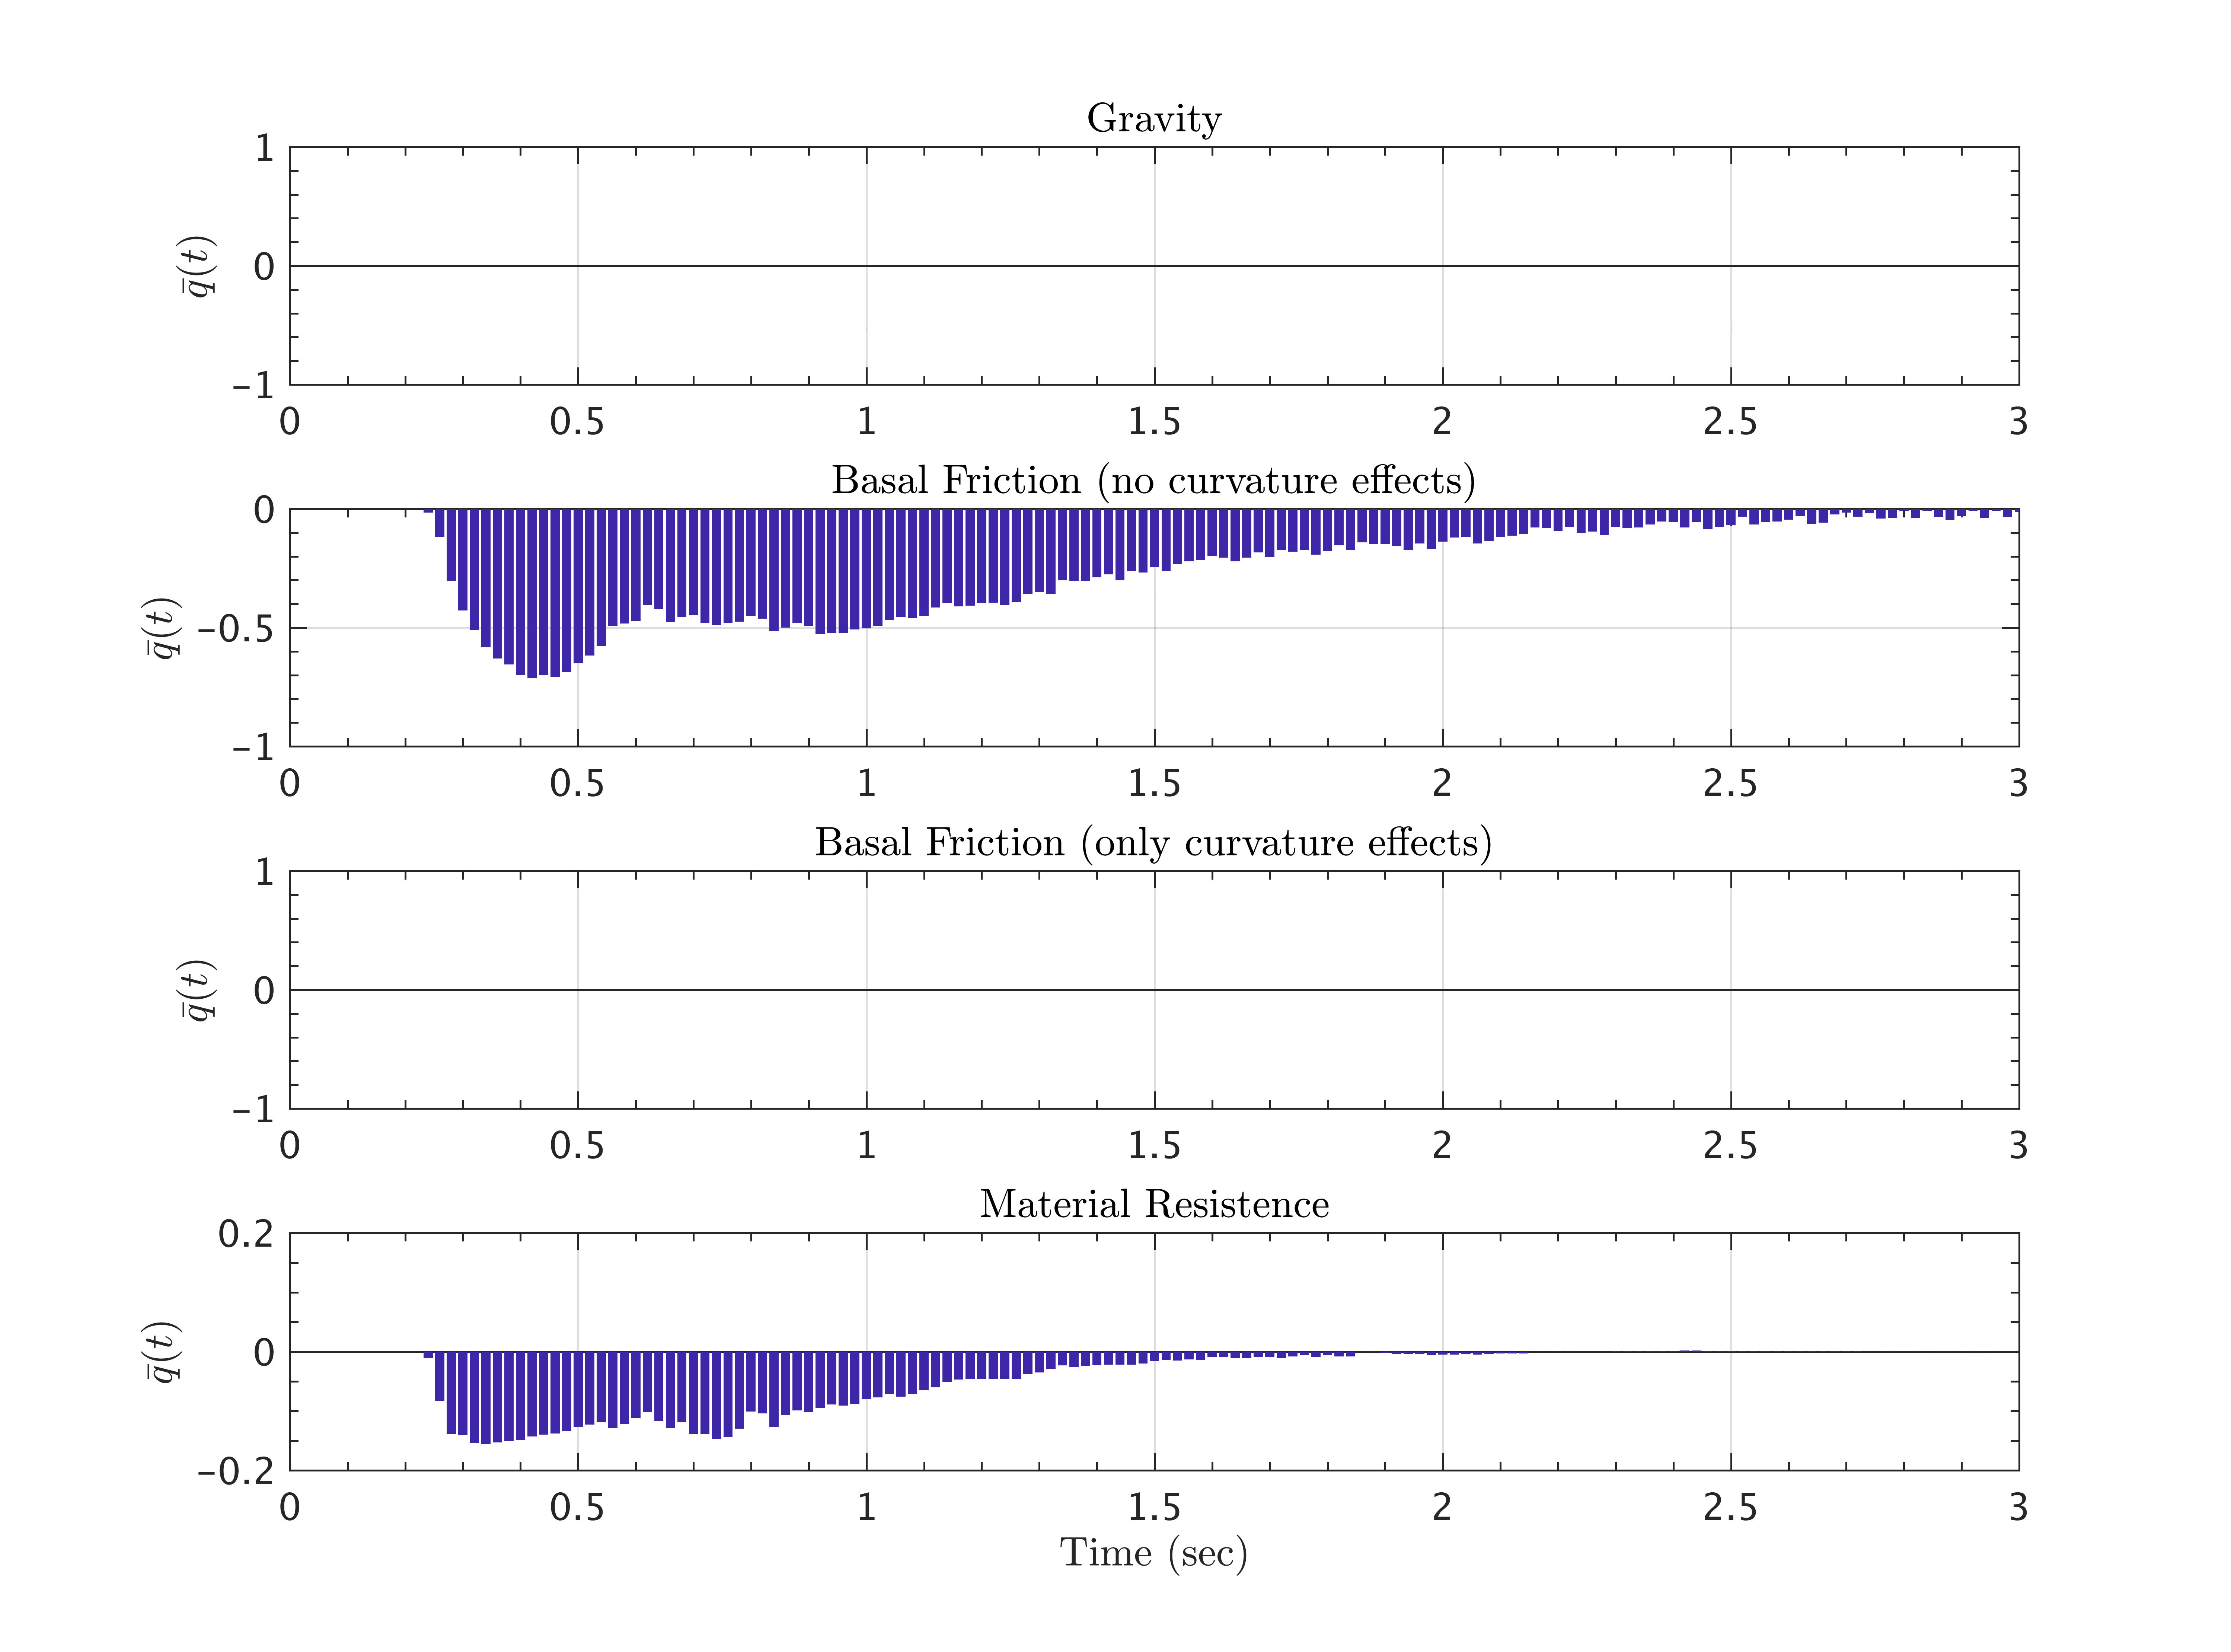
\includegraphics[width=1\textwidth]{InclinedPlane/LocalRecords/ContribF8_V_y.png}
                \subcaption{$x=-0.35, \ y=0.0$, middle point on inclined plane.}
                \label{fig:Ramp-Vy2}
        \end{minipage}

        \begin{minipage}[b]{0.5\linewidth}
                \centering
                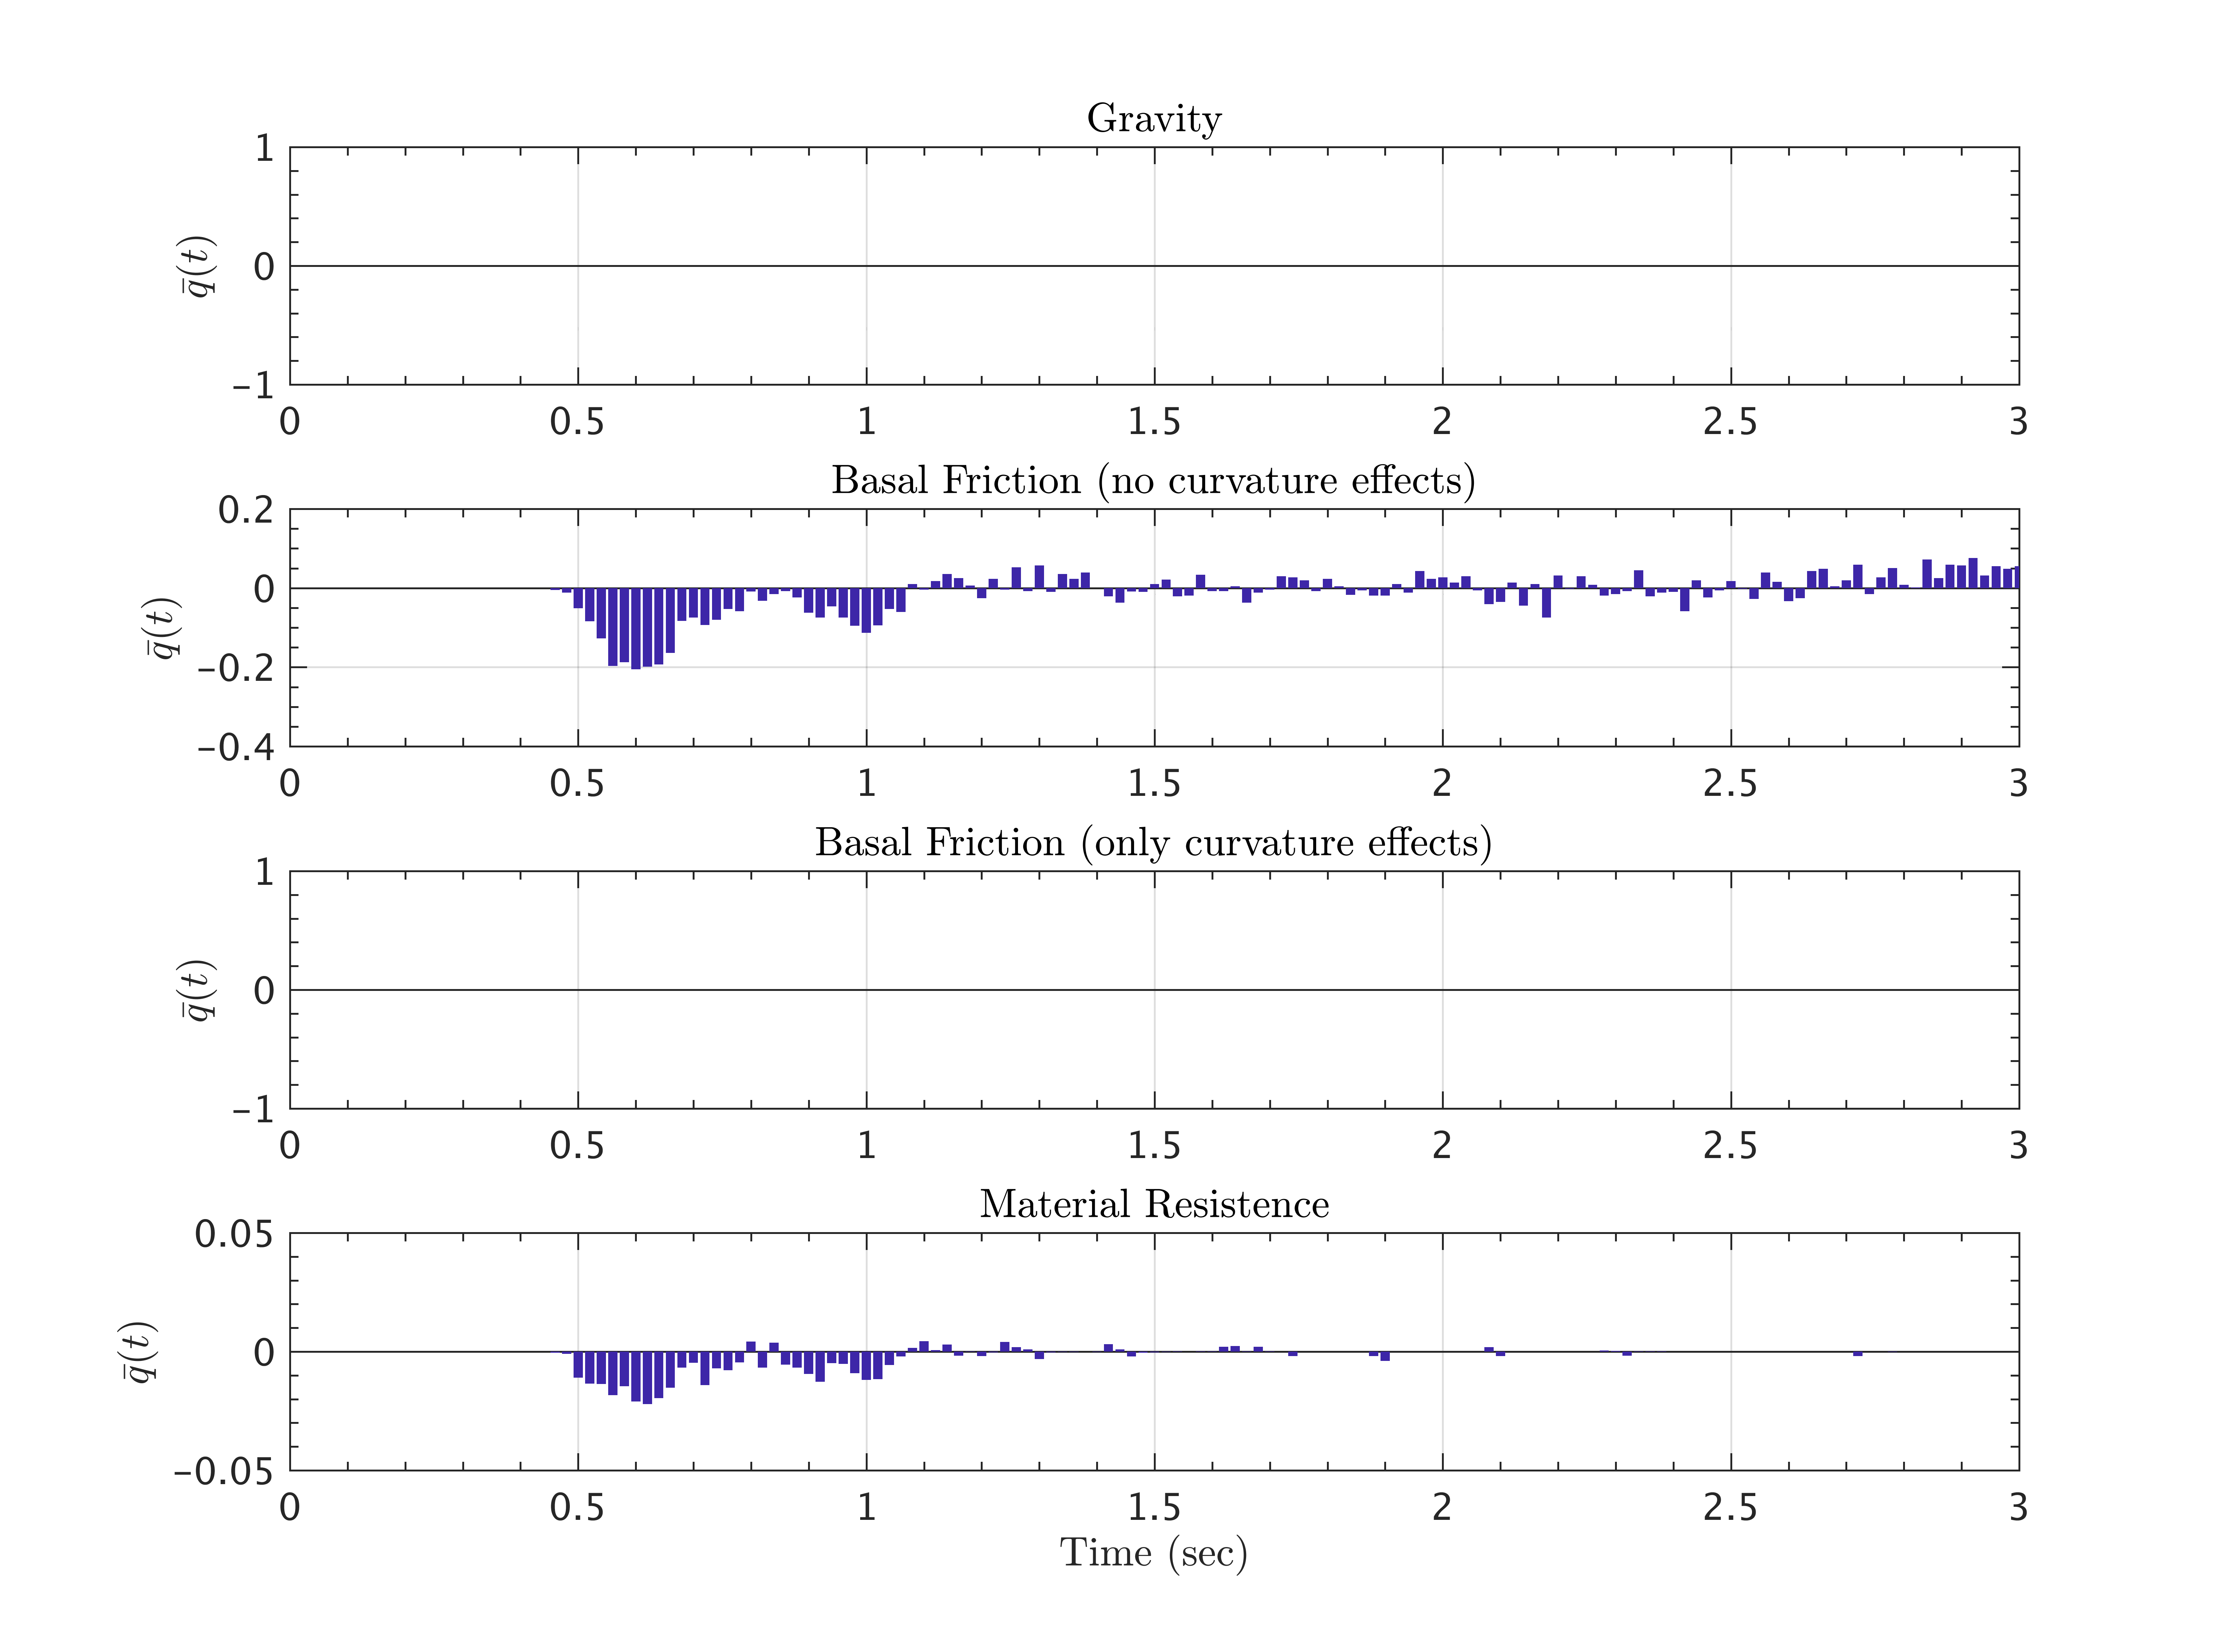
\includegraphics[width=1\textwidth]{InclinedPlane/LocalRecords/ContribF15_V_y.png}
                \subcaption{$x=0, \ y=0$, inclined and runout planes' joint location.}
                \label{fig:Ramp-Vy3}
        \end{minipage}
        \begin{minipage}[b]{0.5\linewidth}
                \centering
                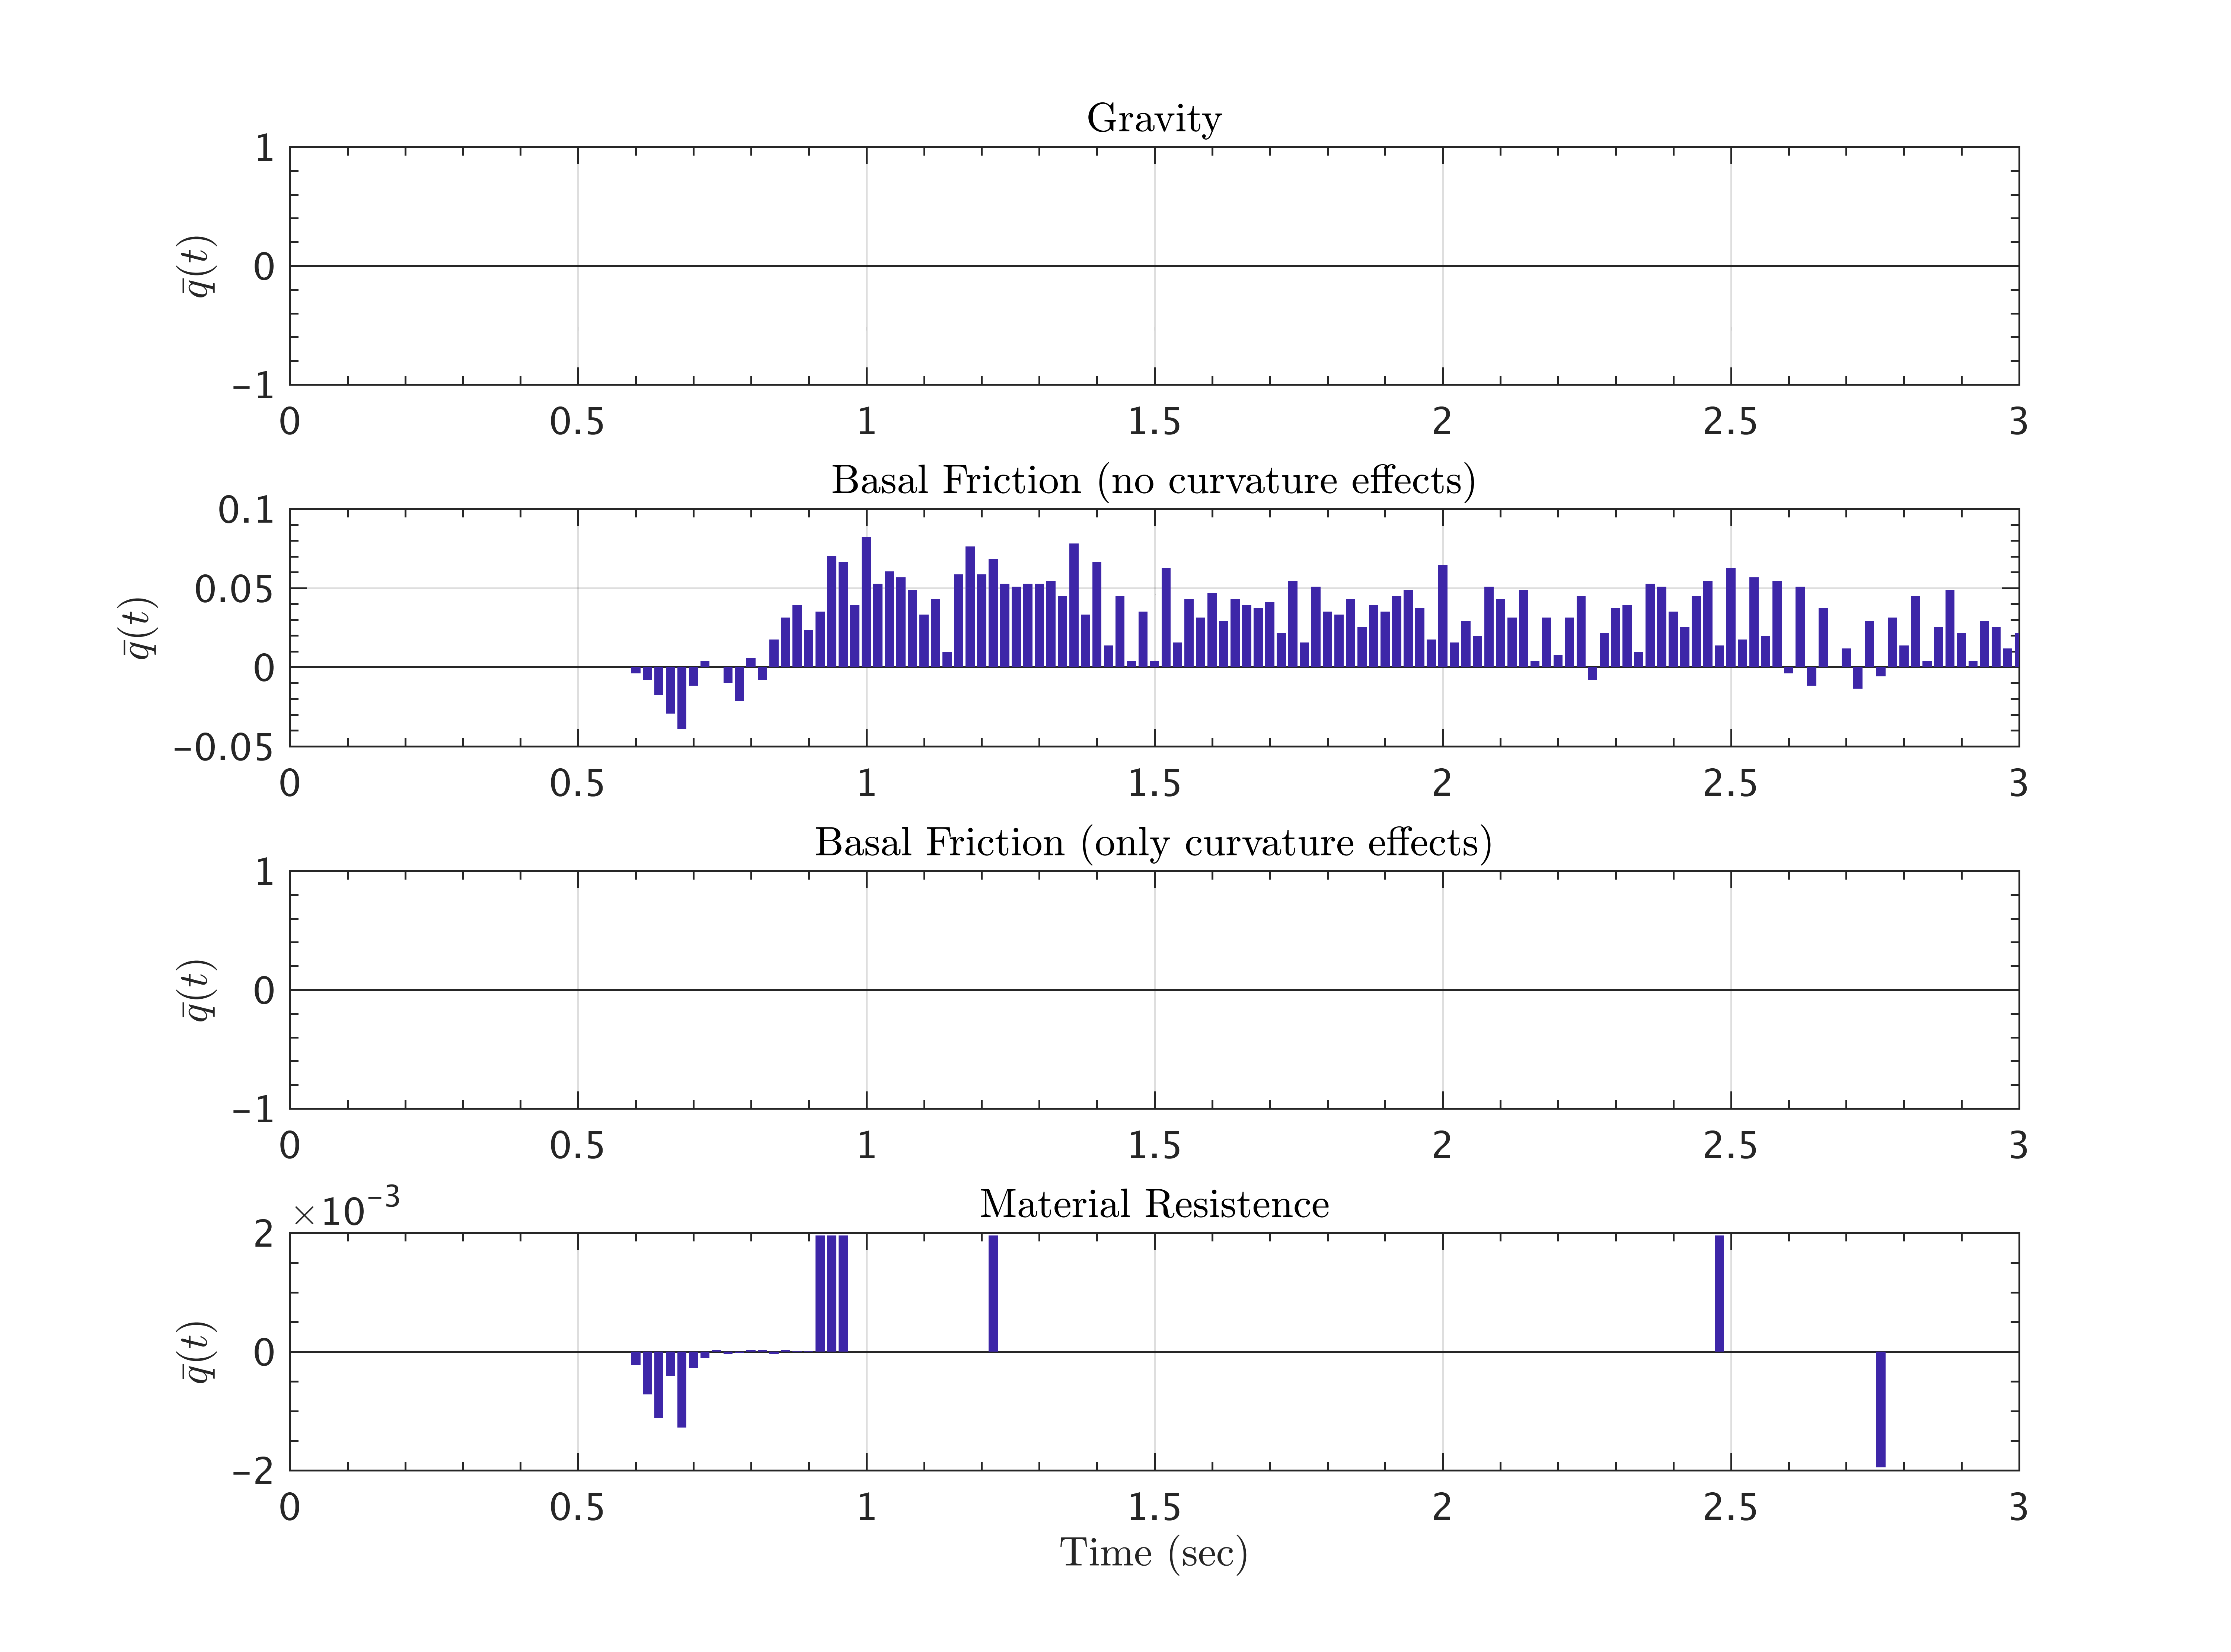
\includegraphics[width=1\textwidth]{InclinedPlane/LocalRecords/ContribF17_V_y.png}
                \subcaption{$x=0.15, \ y=0.0$, a location on runout plane.}
                \label{fig:Ramp-Vy4}
        \end{minipage}
        \caption{Time history of mean values for force impact quotients, $\bar{q}_i(t)$, along the lateral direction, Voellmy-Salm model.}
        \label{fig:Ramp-Vy}
\end{figure}

\subsubsection{Temporal Records for Bulk of flowing material}

\begin{figure}[H]
        \begin{minipage}[b]{0.5\linewidth}
                \centering
                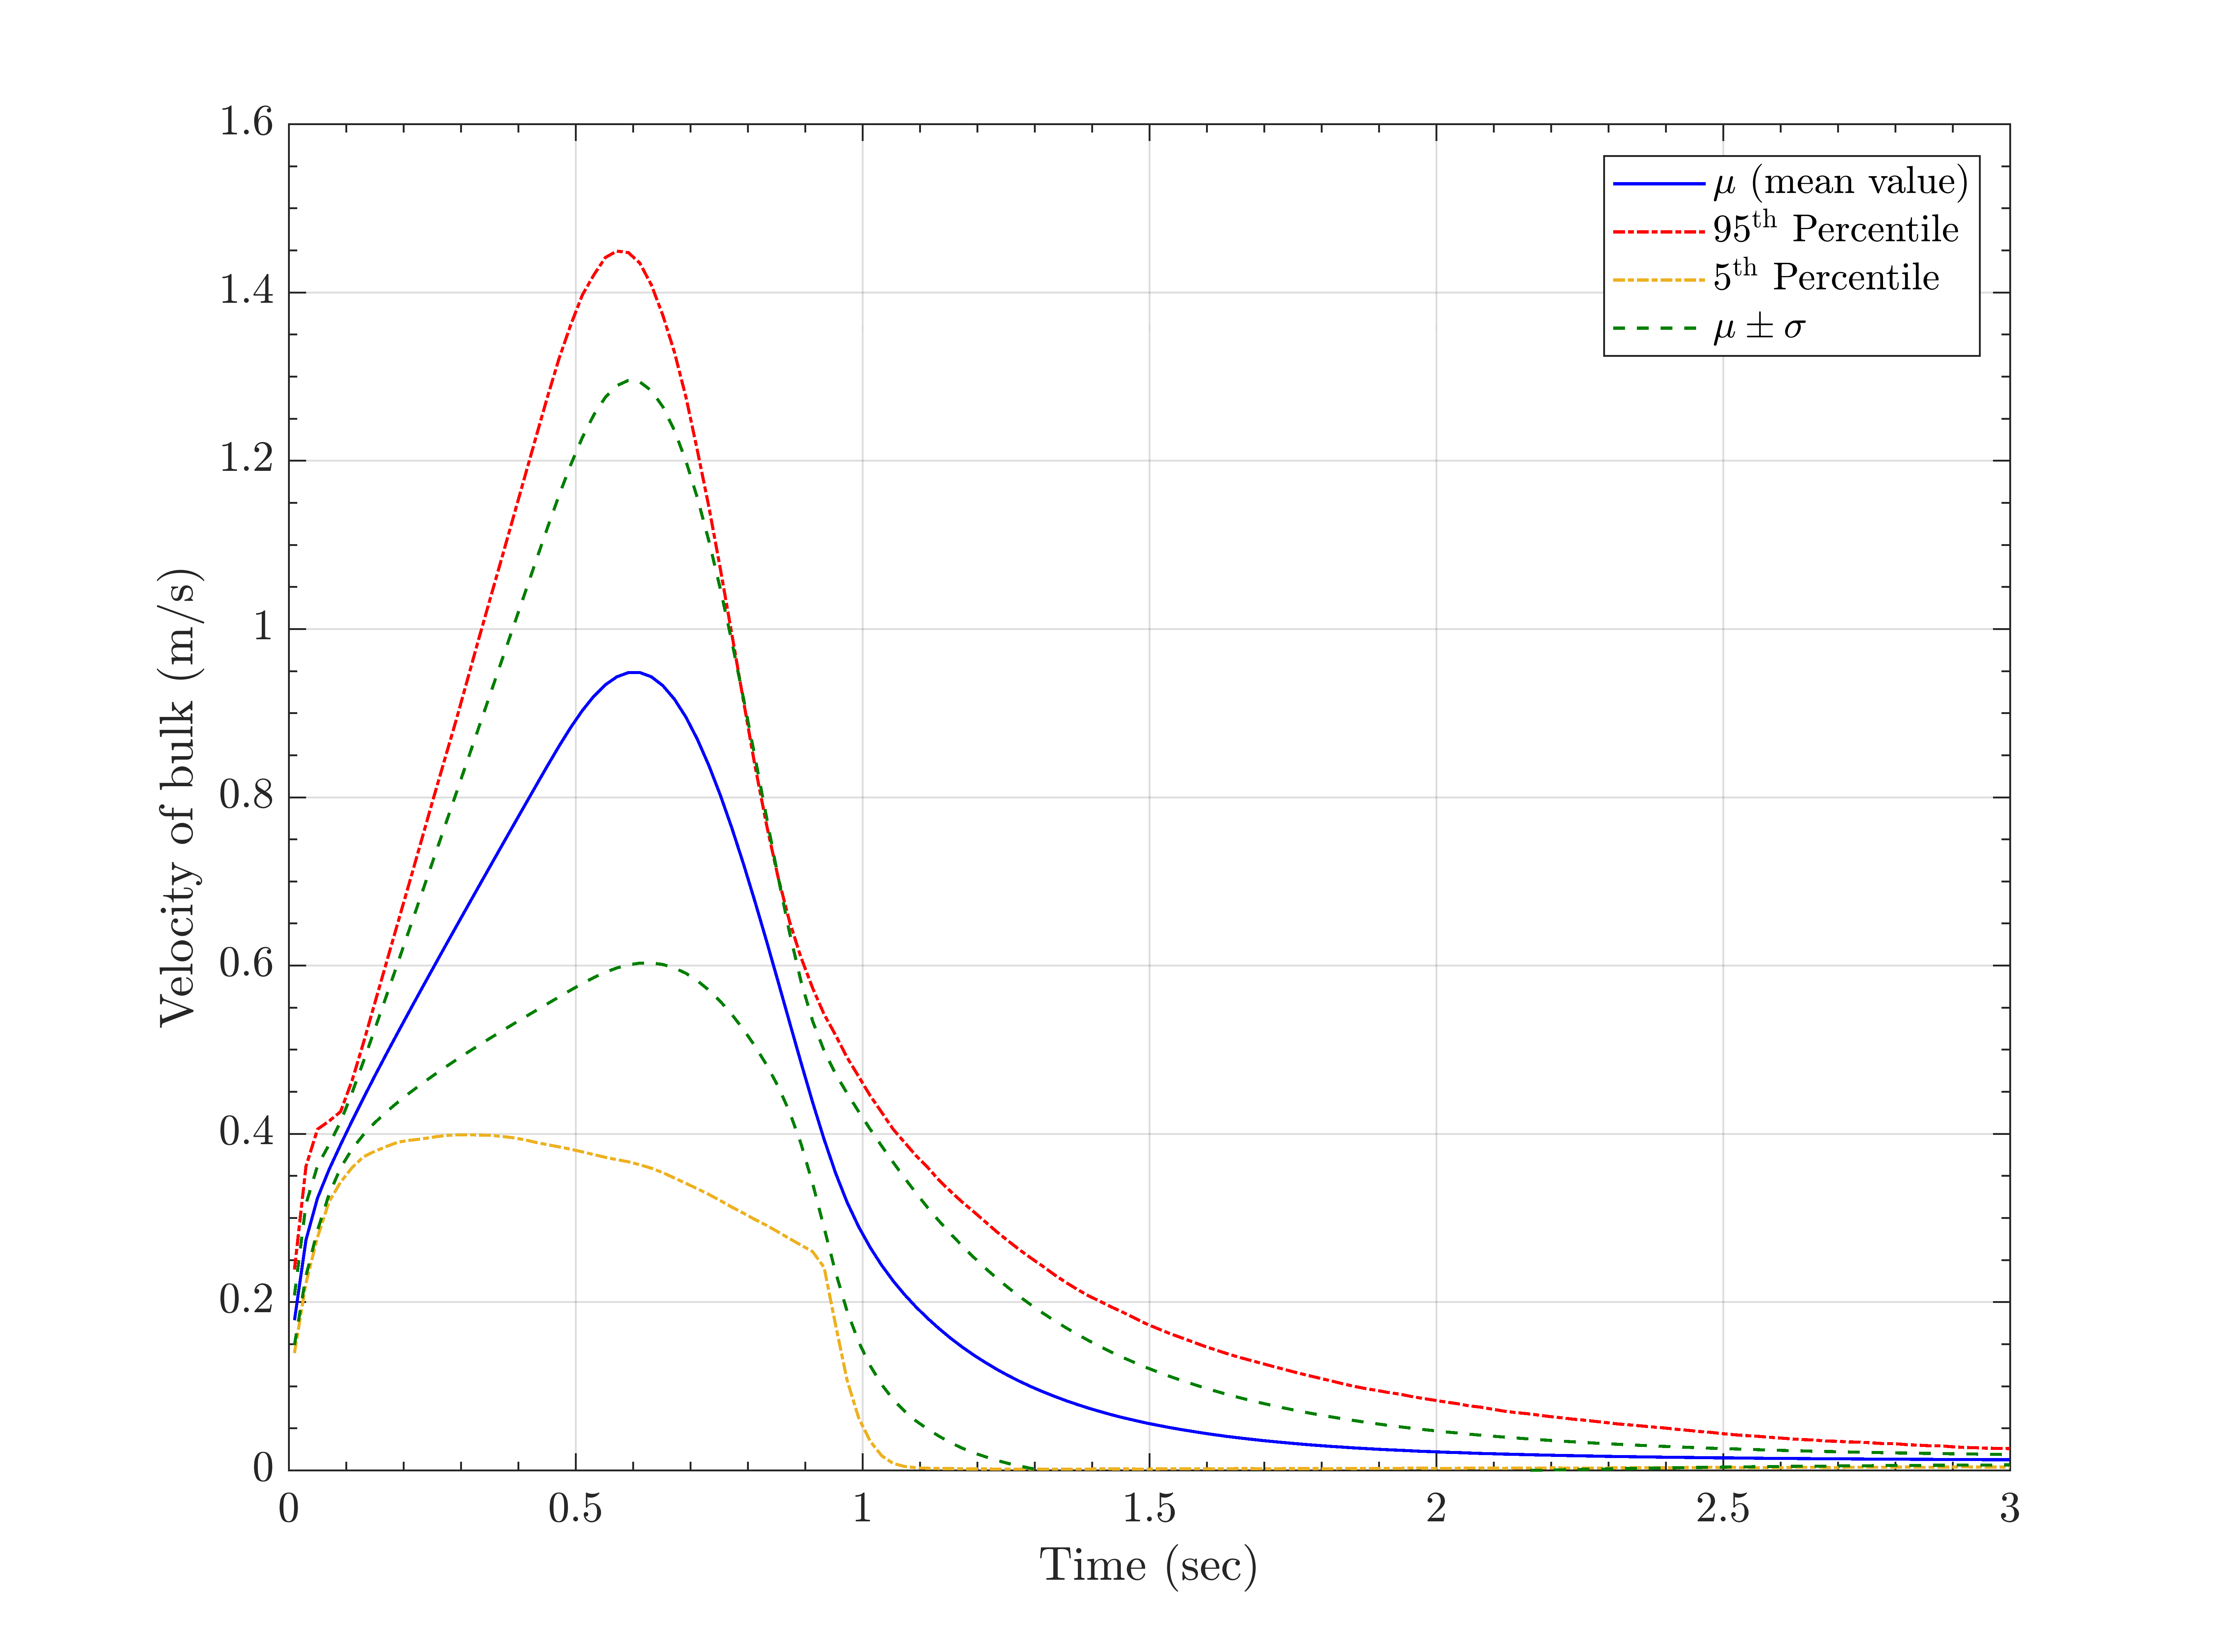
\includegraphics[width=1\textwidth]{InclinedPlane/GlobalRecords/C_Global_Vel.png}
                \subcaption{Mohr-Coulomb model.}
                \label{fig:Ramp-SP-Vel-C}
        \end{minipage}
        \begin{minipage}[b]{0.5\linewidth}
                \centering
                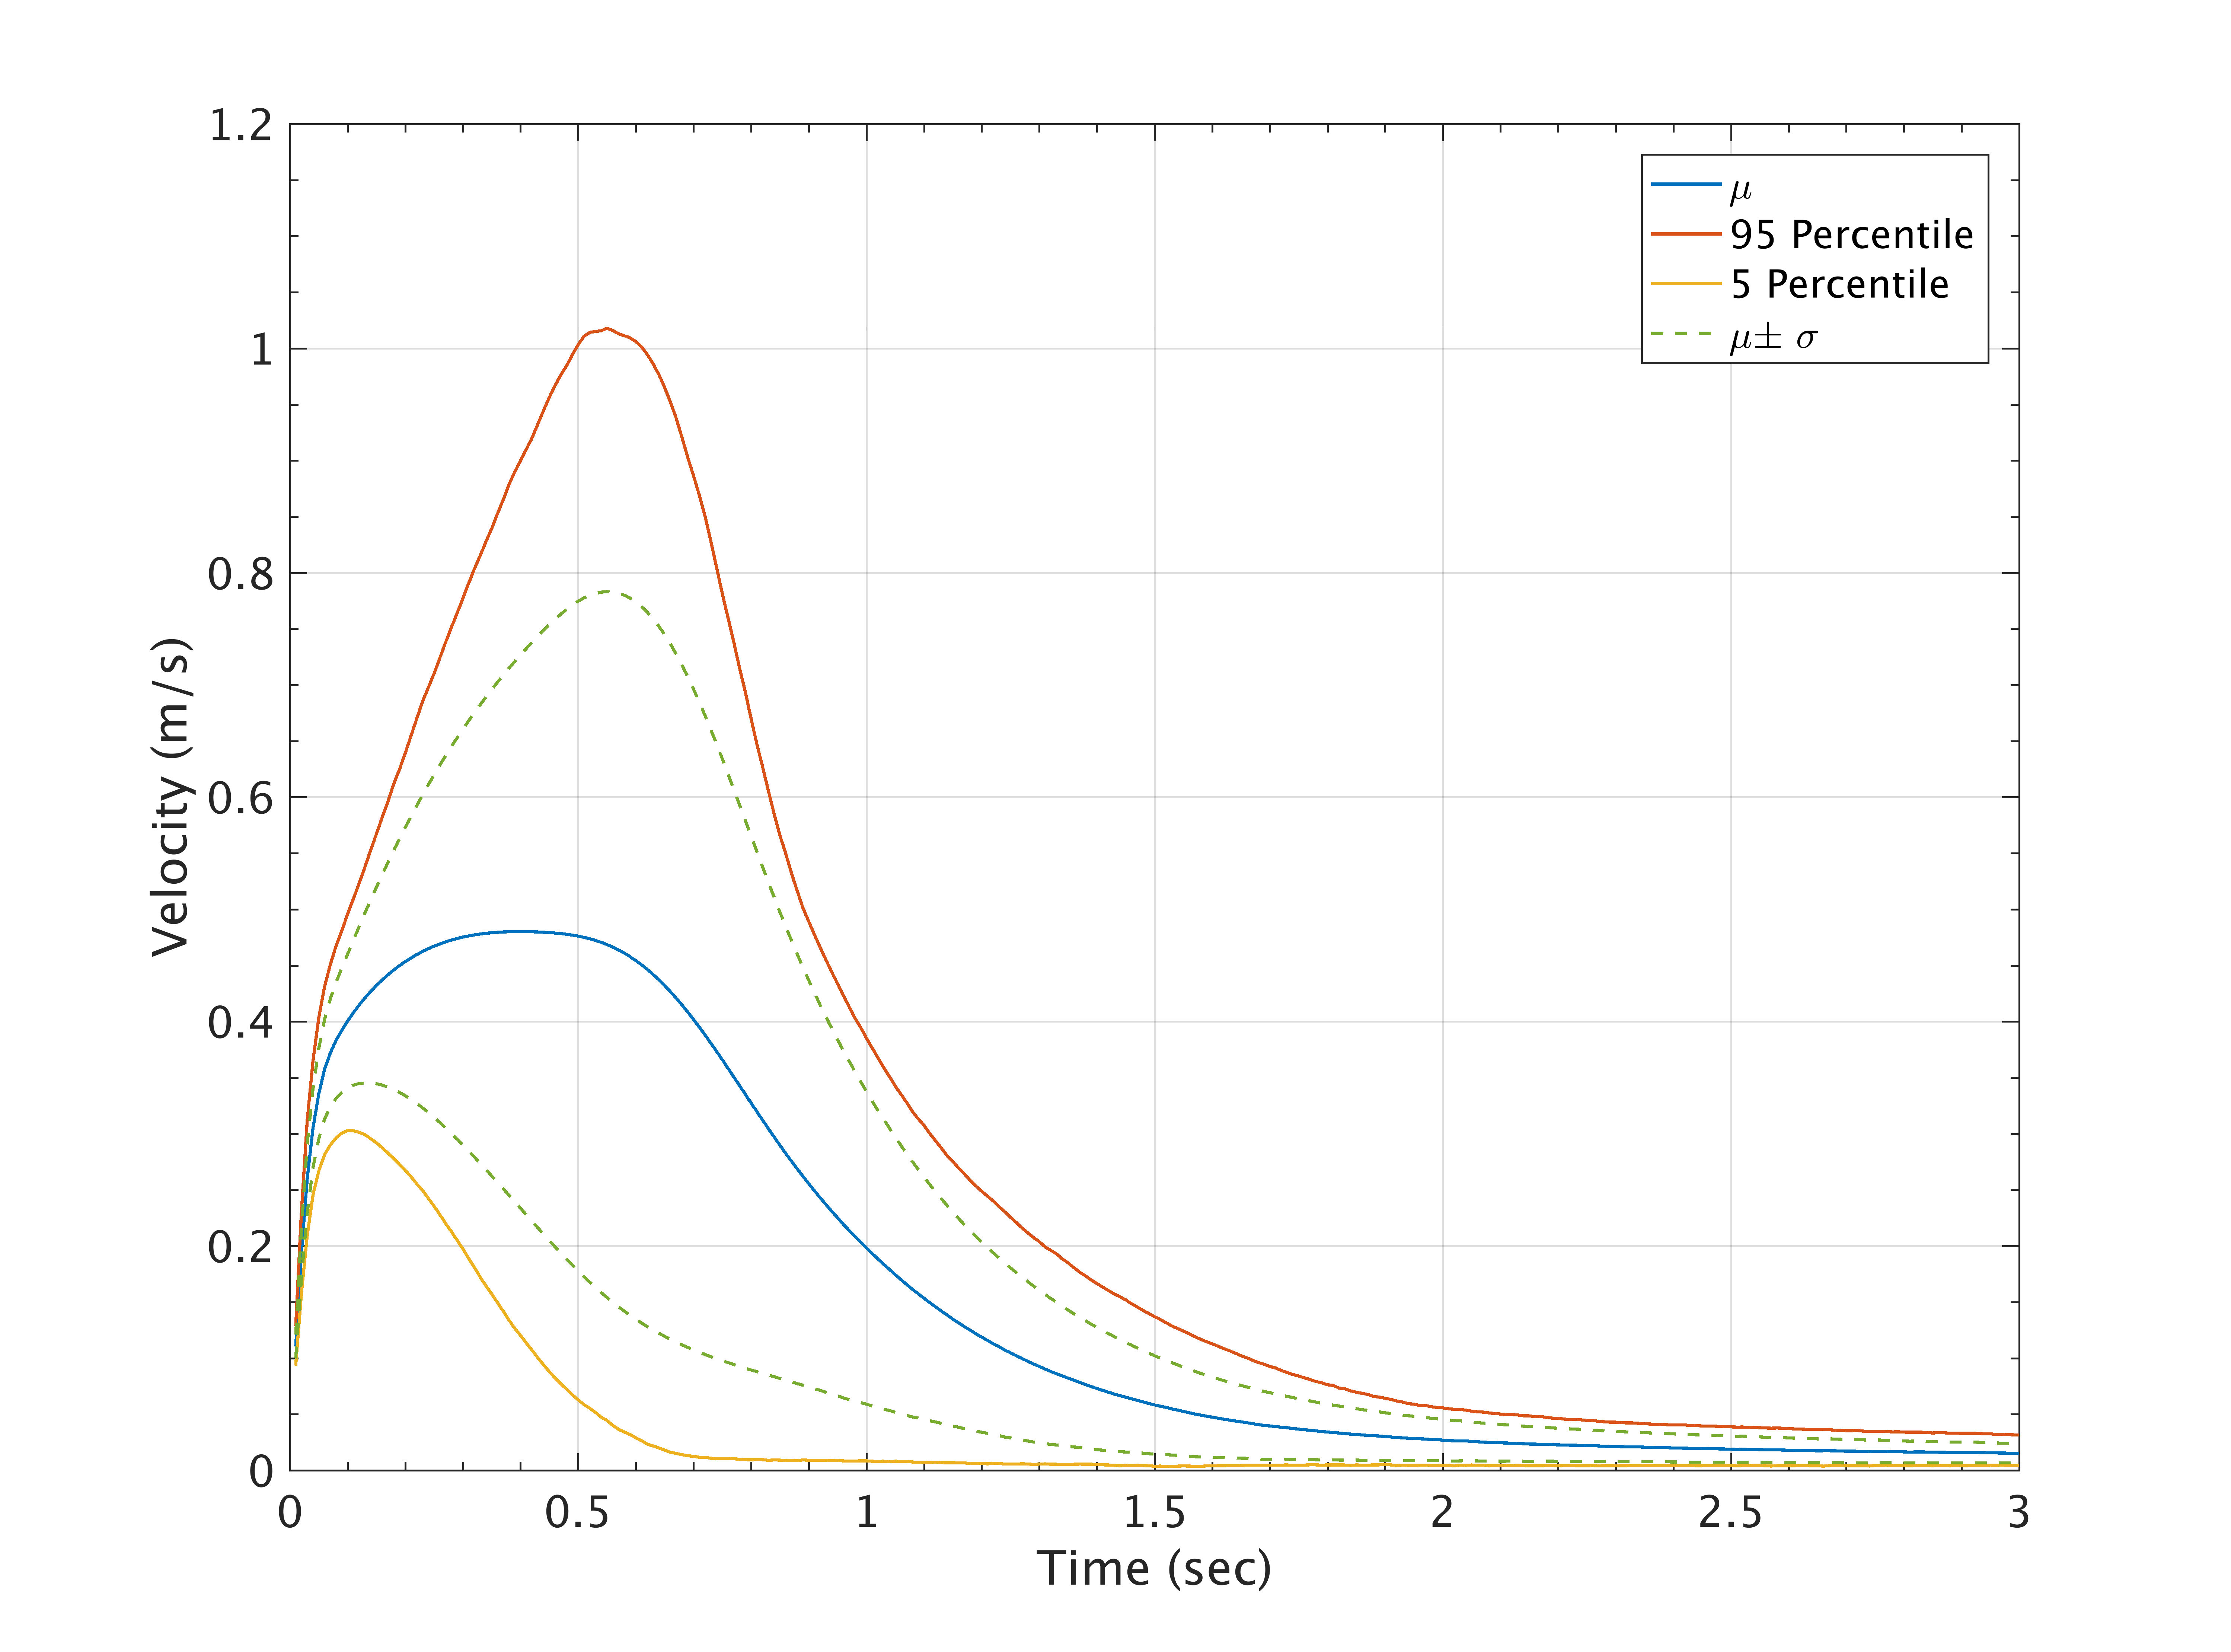
\includegraphics[width=1\textwidth]{InclinedPlane/GlobalRecords/P_Global_Vel.png}
                \subcaption{Pouliquen-Forterre model.}
                \label{fig:Ramp-SP-Vel-P}
        \end{minipage}

        \begin{minipage}[b]{1\linewidth}
                \centering
                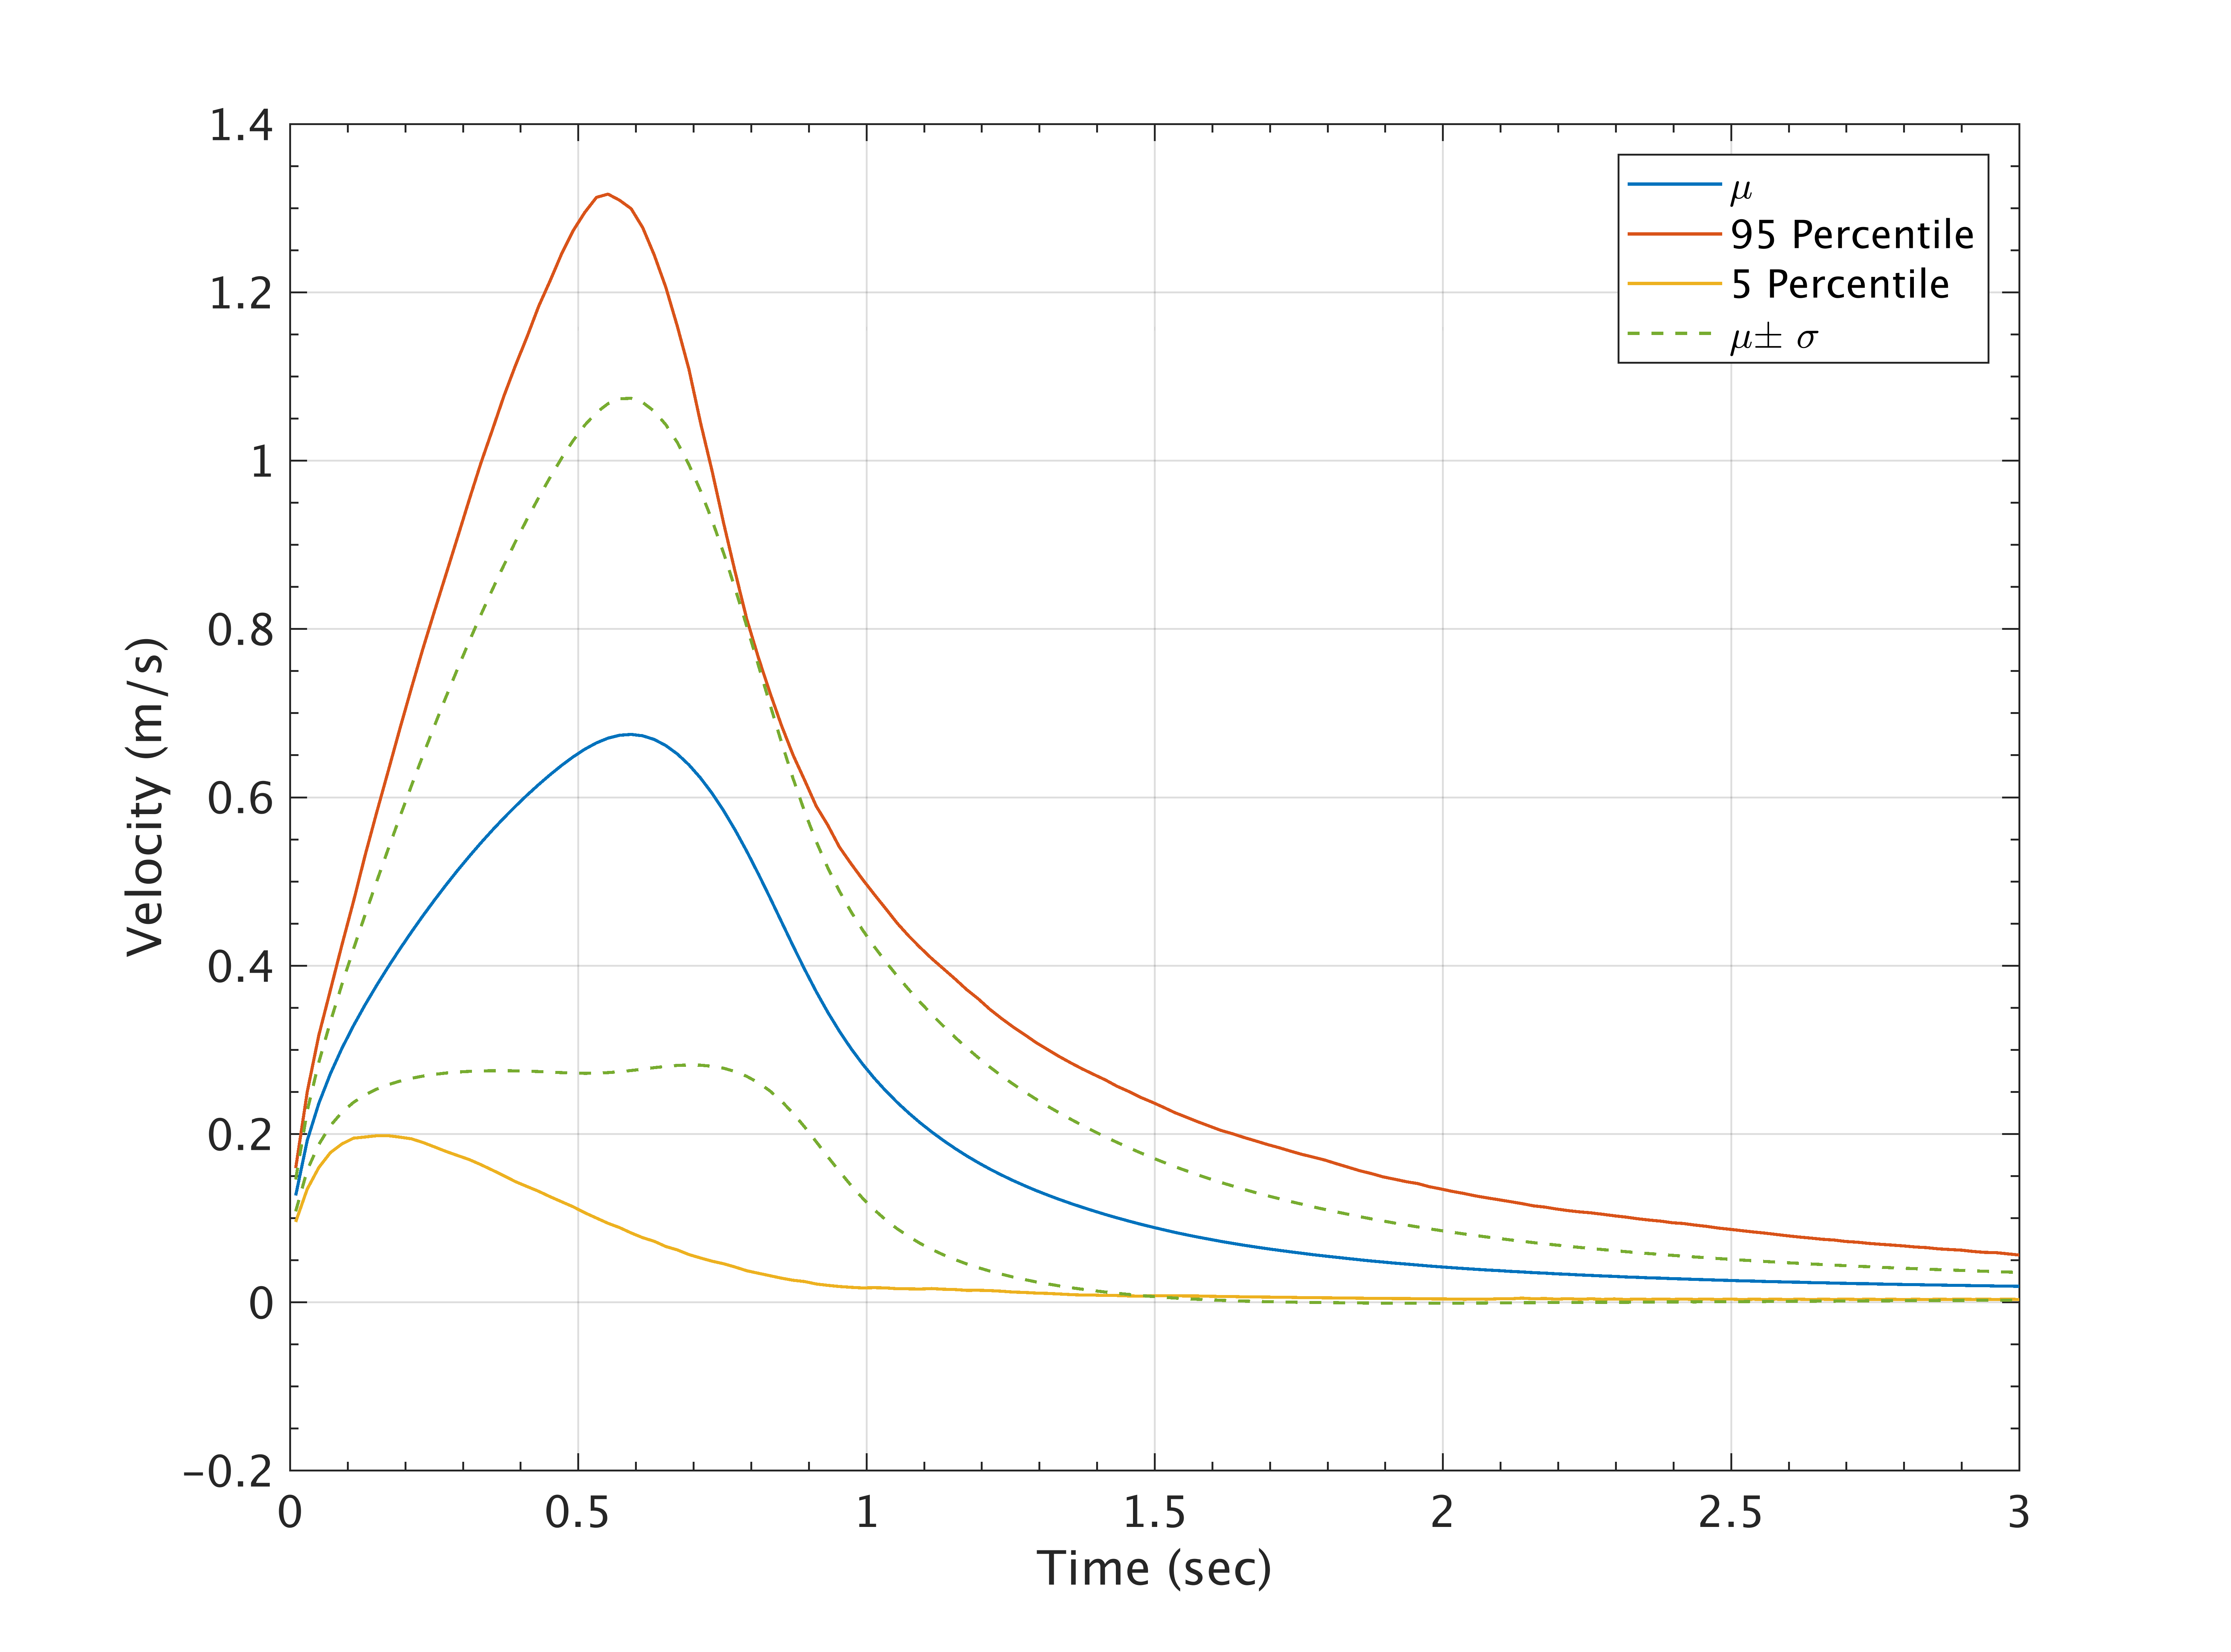
\includegraphics[width=0.5\textwidth]{InclinedPlane/GlobalRecords/V_Global_Vel.png}
                \subcaption{Voellmy-Salm model.}
                \label{fig:Ramp-SP-Vel-V}
        \end{minipage}
        \caption{Full statistics of velocity records for bulk of material.}
        \label{fig:Ramp-SP-Vel}
\end{figure}

\begin{figure}[H]
        \begin{minipage}[b]{0.5\linewidth}
                \centering
                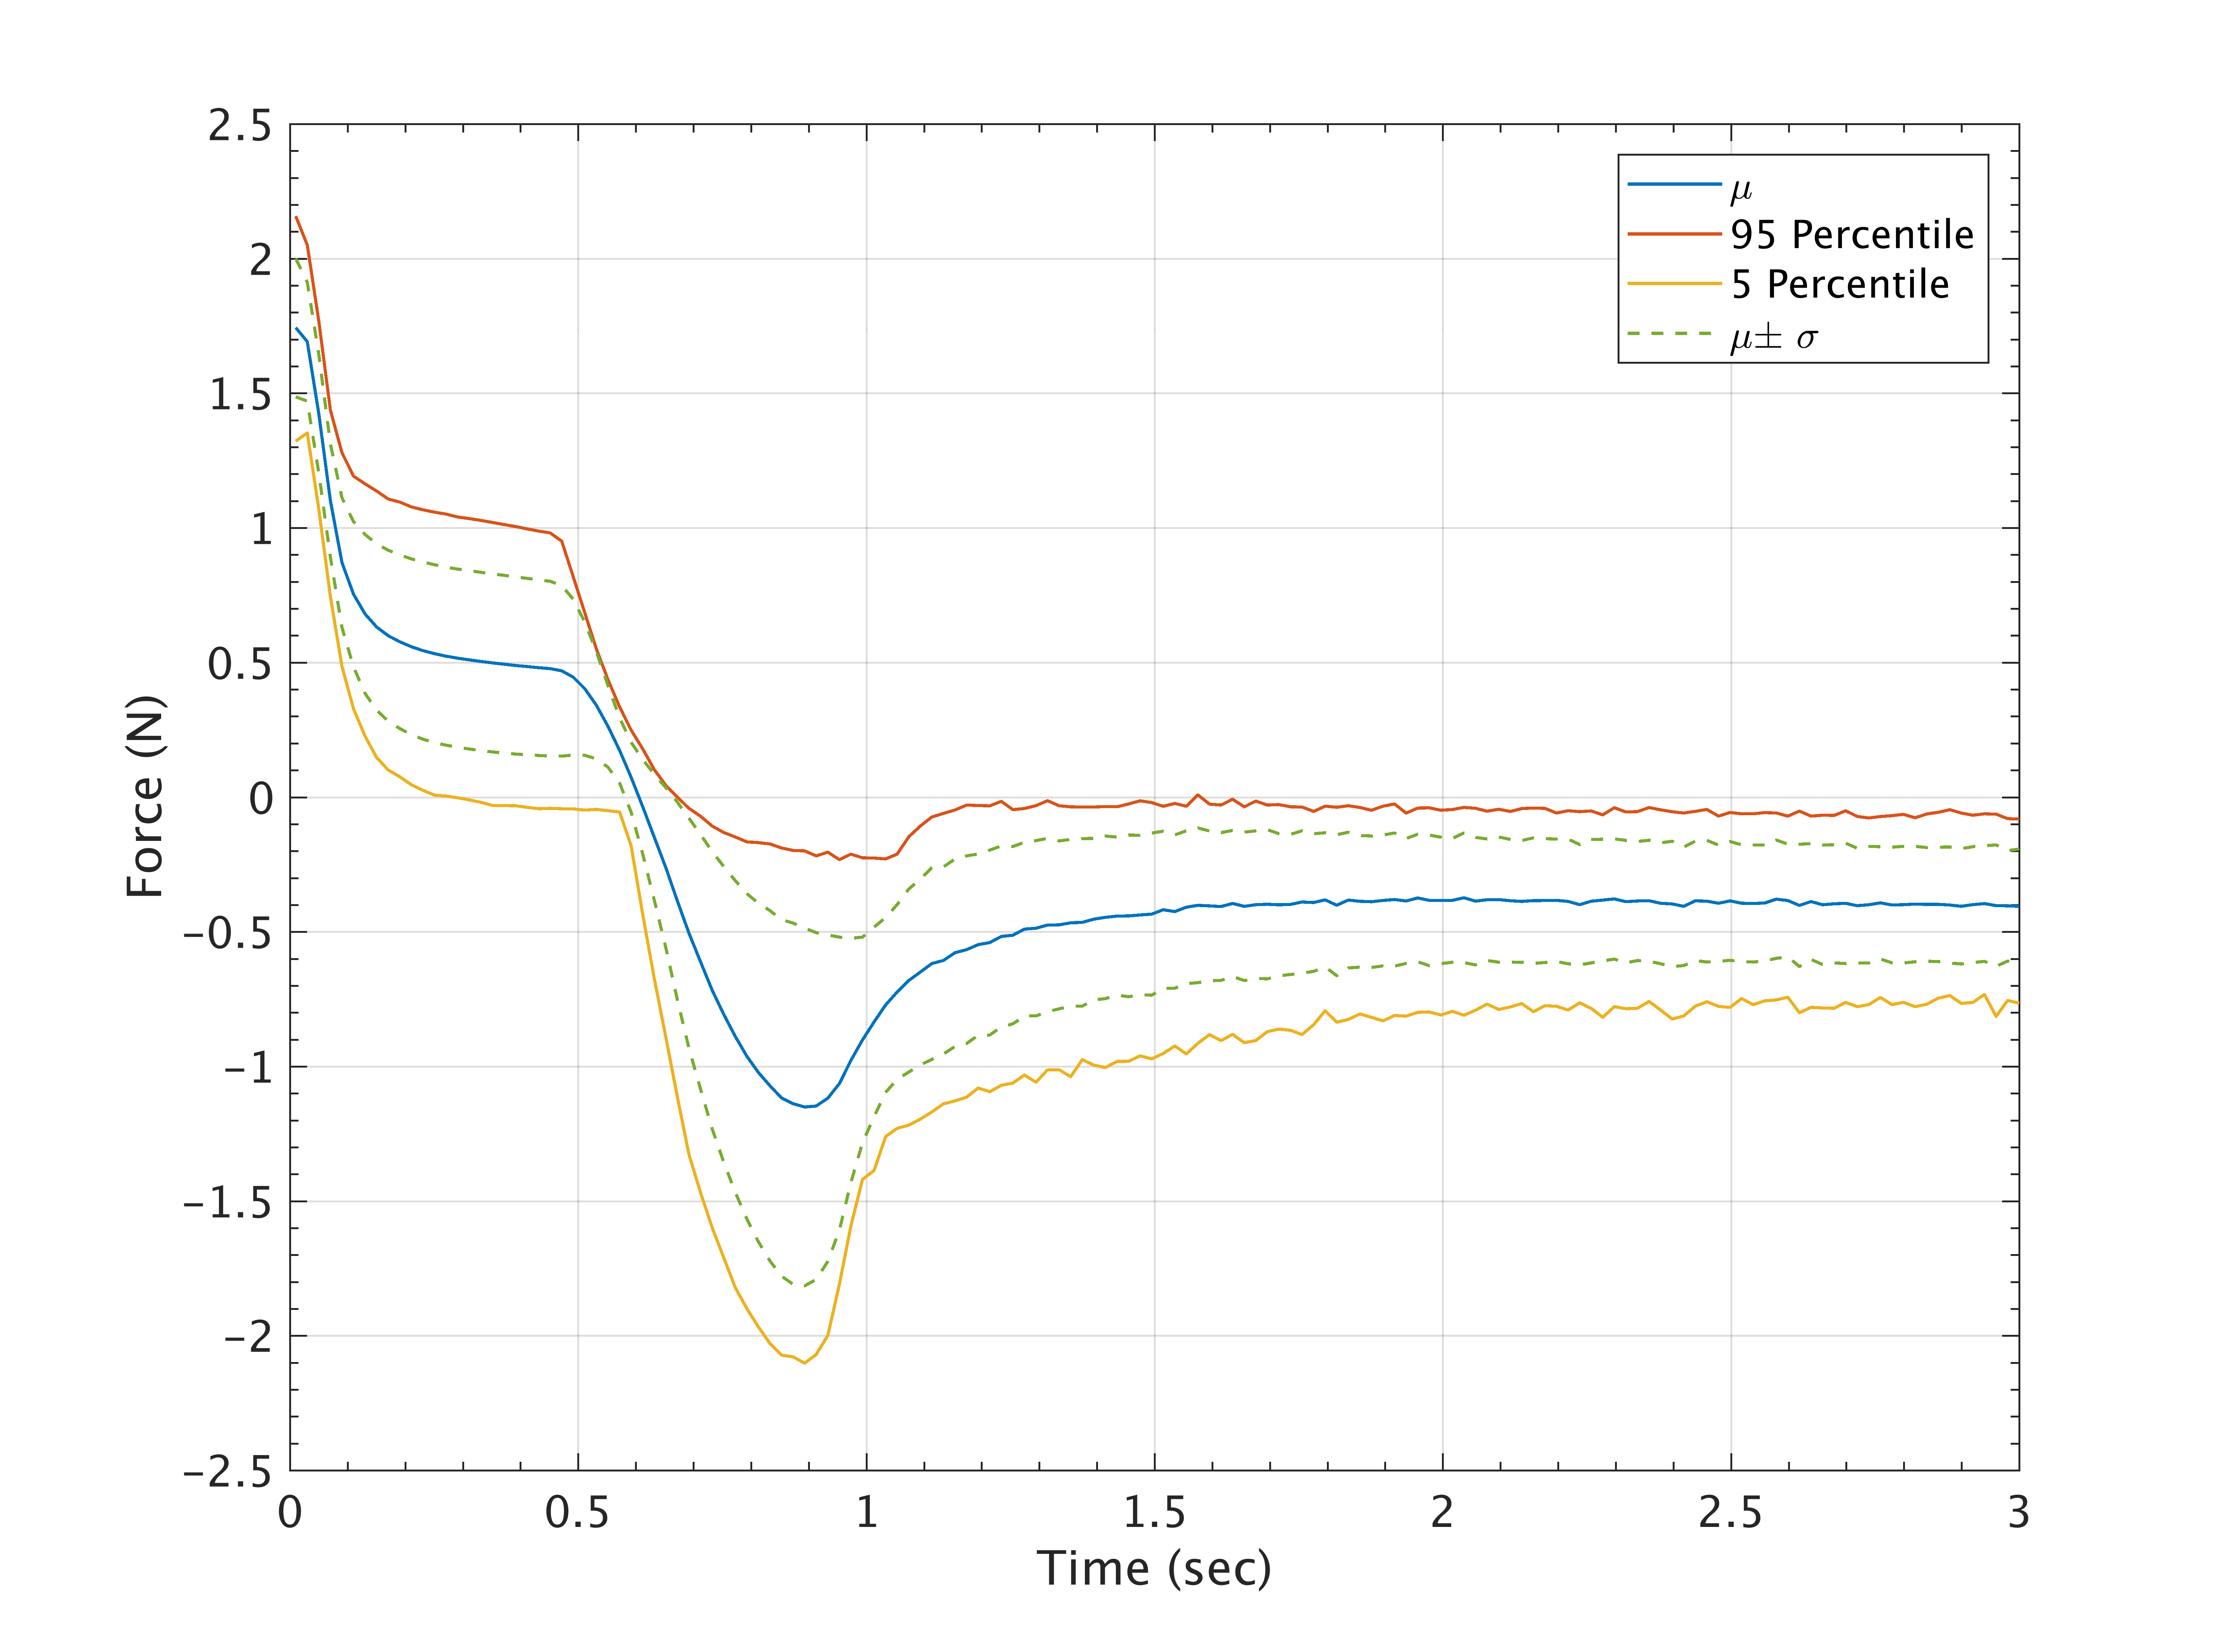
\includegraphics[width=1\textwidth]{InclinedPlane/GlobalRecords/C_Global_Fx.png}
                \subcaption{Mohr-Coulomb model, runout direction.}
                \label{fig:Ramp-SP-Fx-C}
        \end{minipage}
        \begin{minipage}[b]{0.5\linewidth}
                \centering
                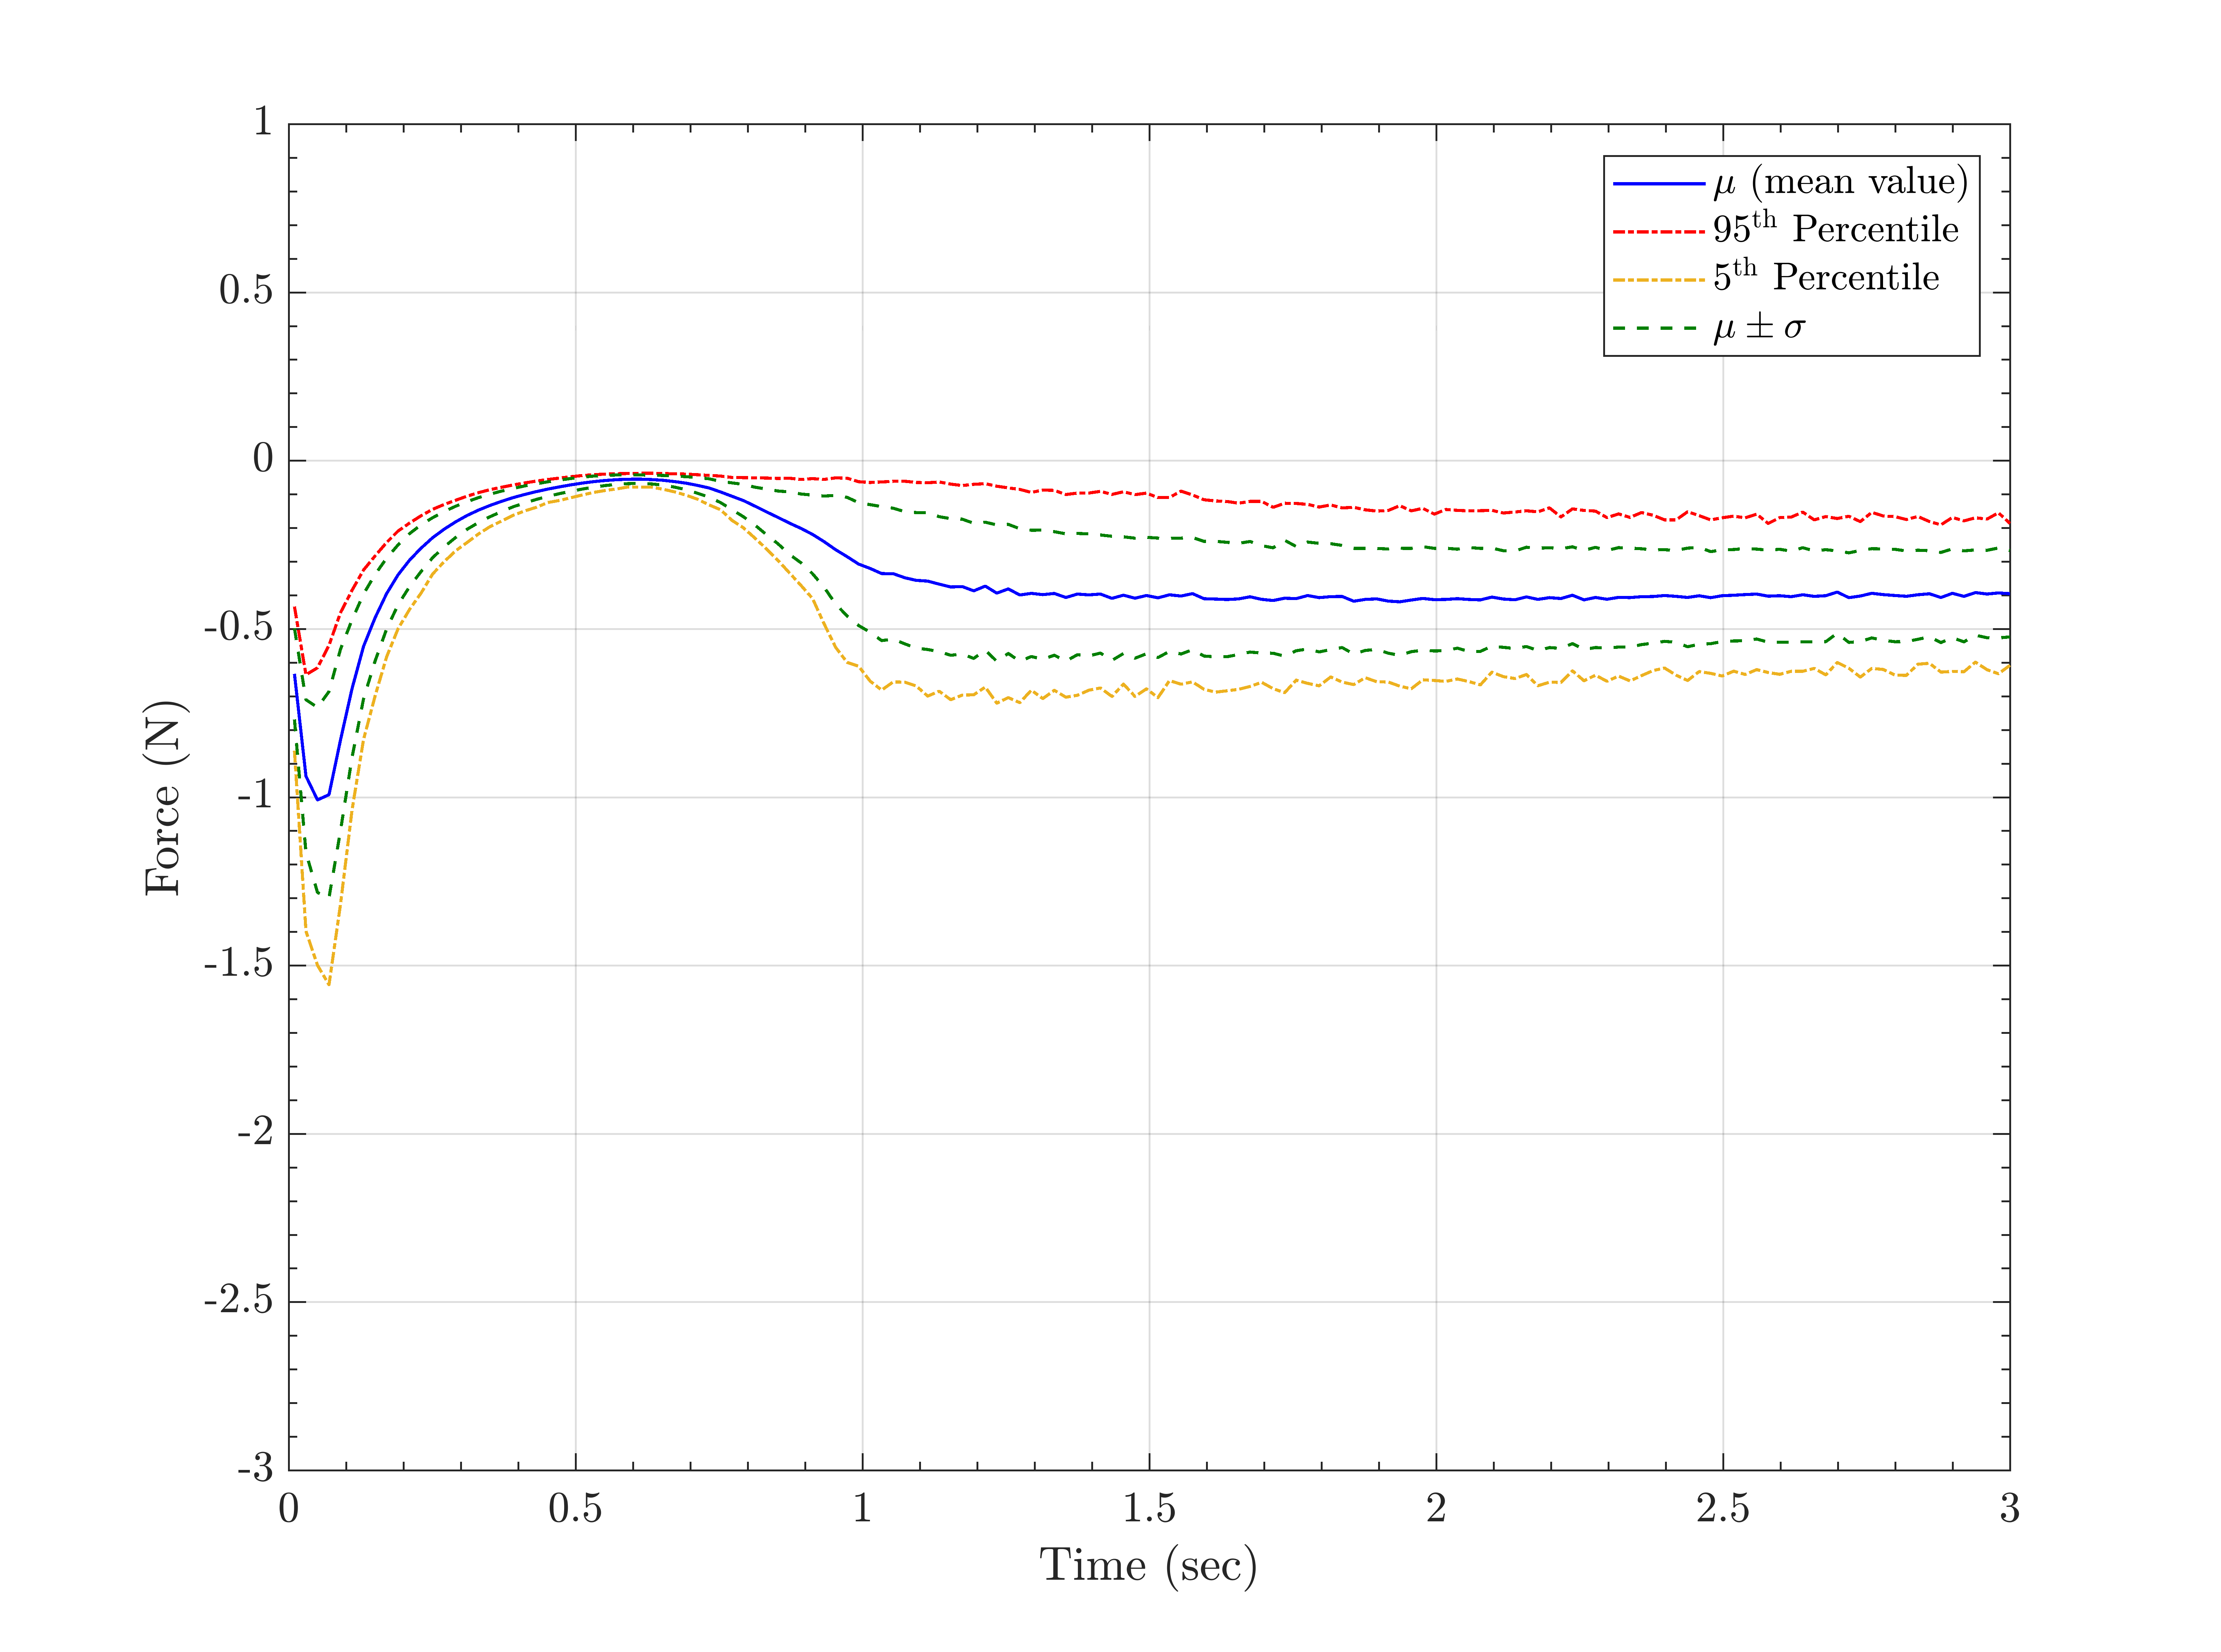
\includegraphics[width=1\textwidth]{InclinedPlane/GlobalRecords/C_Global_Fy.png}
                \subcaption{Mohr-Coulomb model, lateral direction.}
                \label{fig:Ramp-SP-Fy-C}
        \end{minipage}
        
        \begin{minipage}[b]{0.5\linewidth}
                \centering
                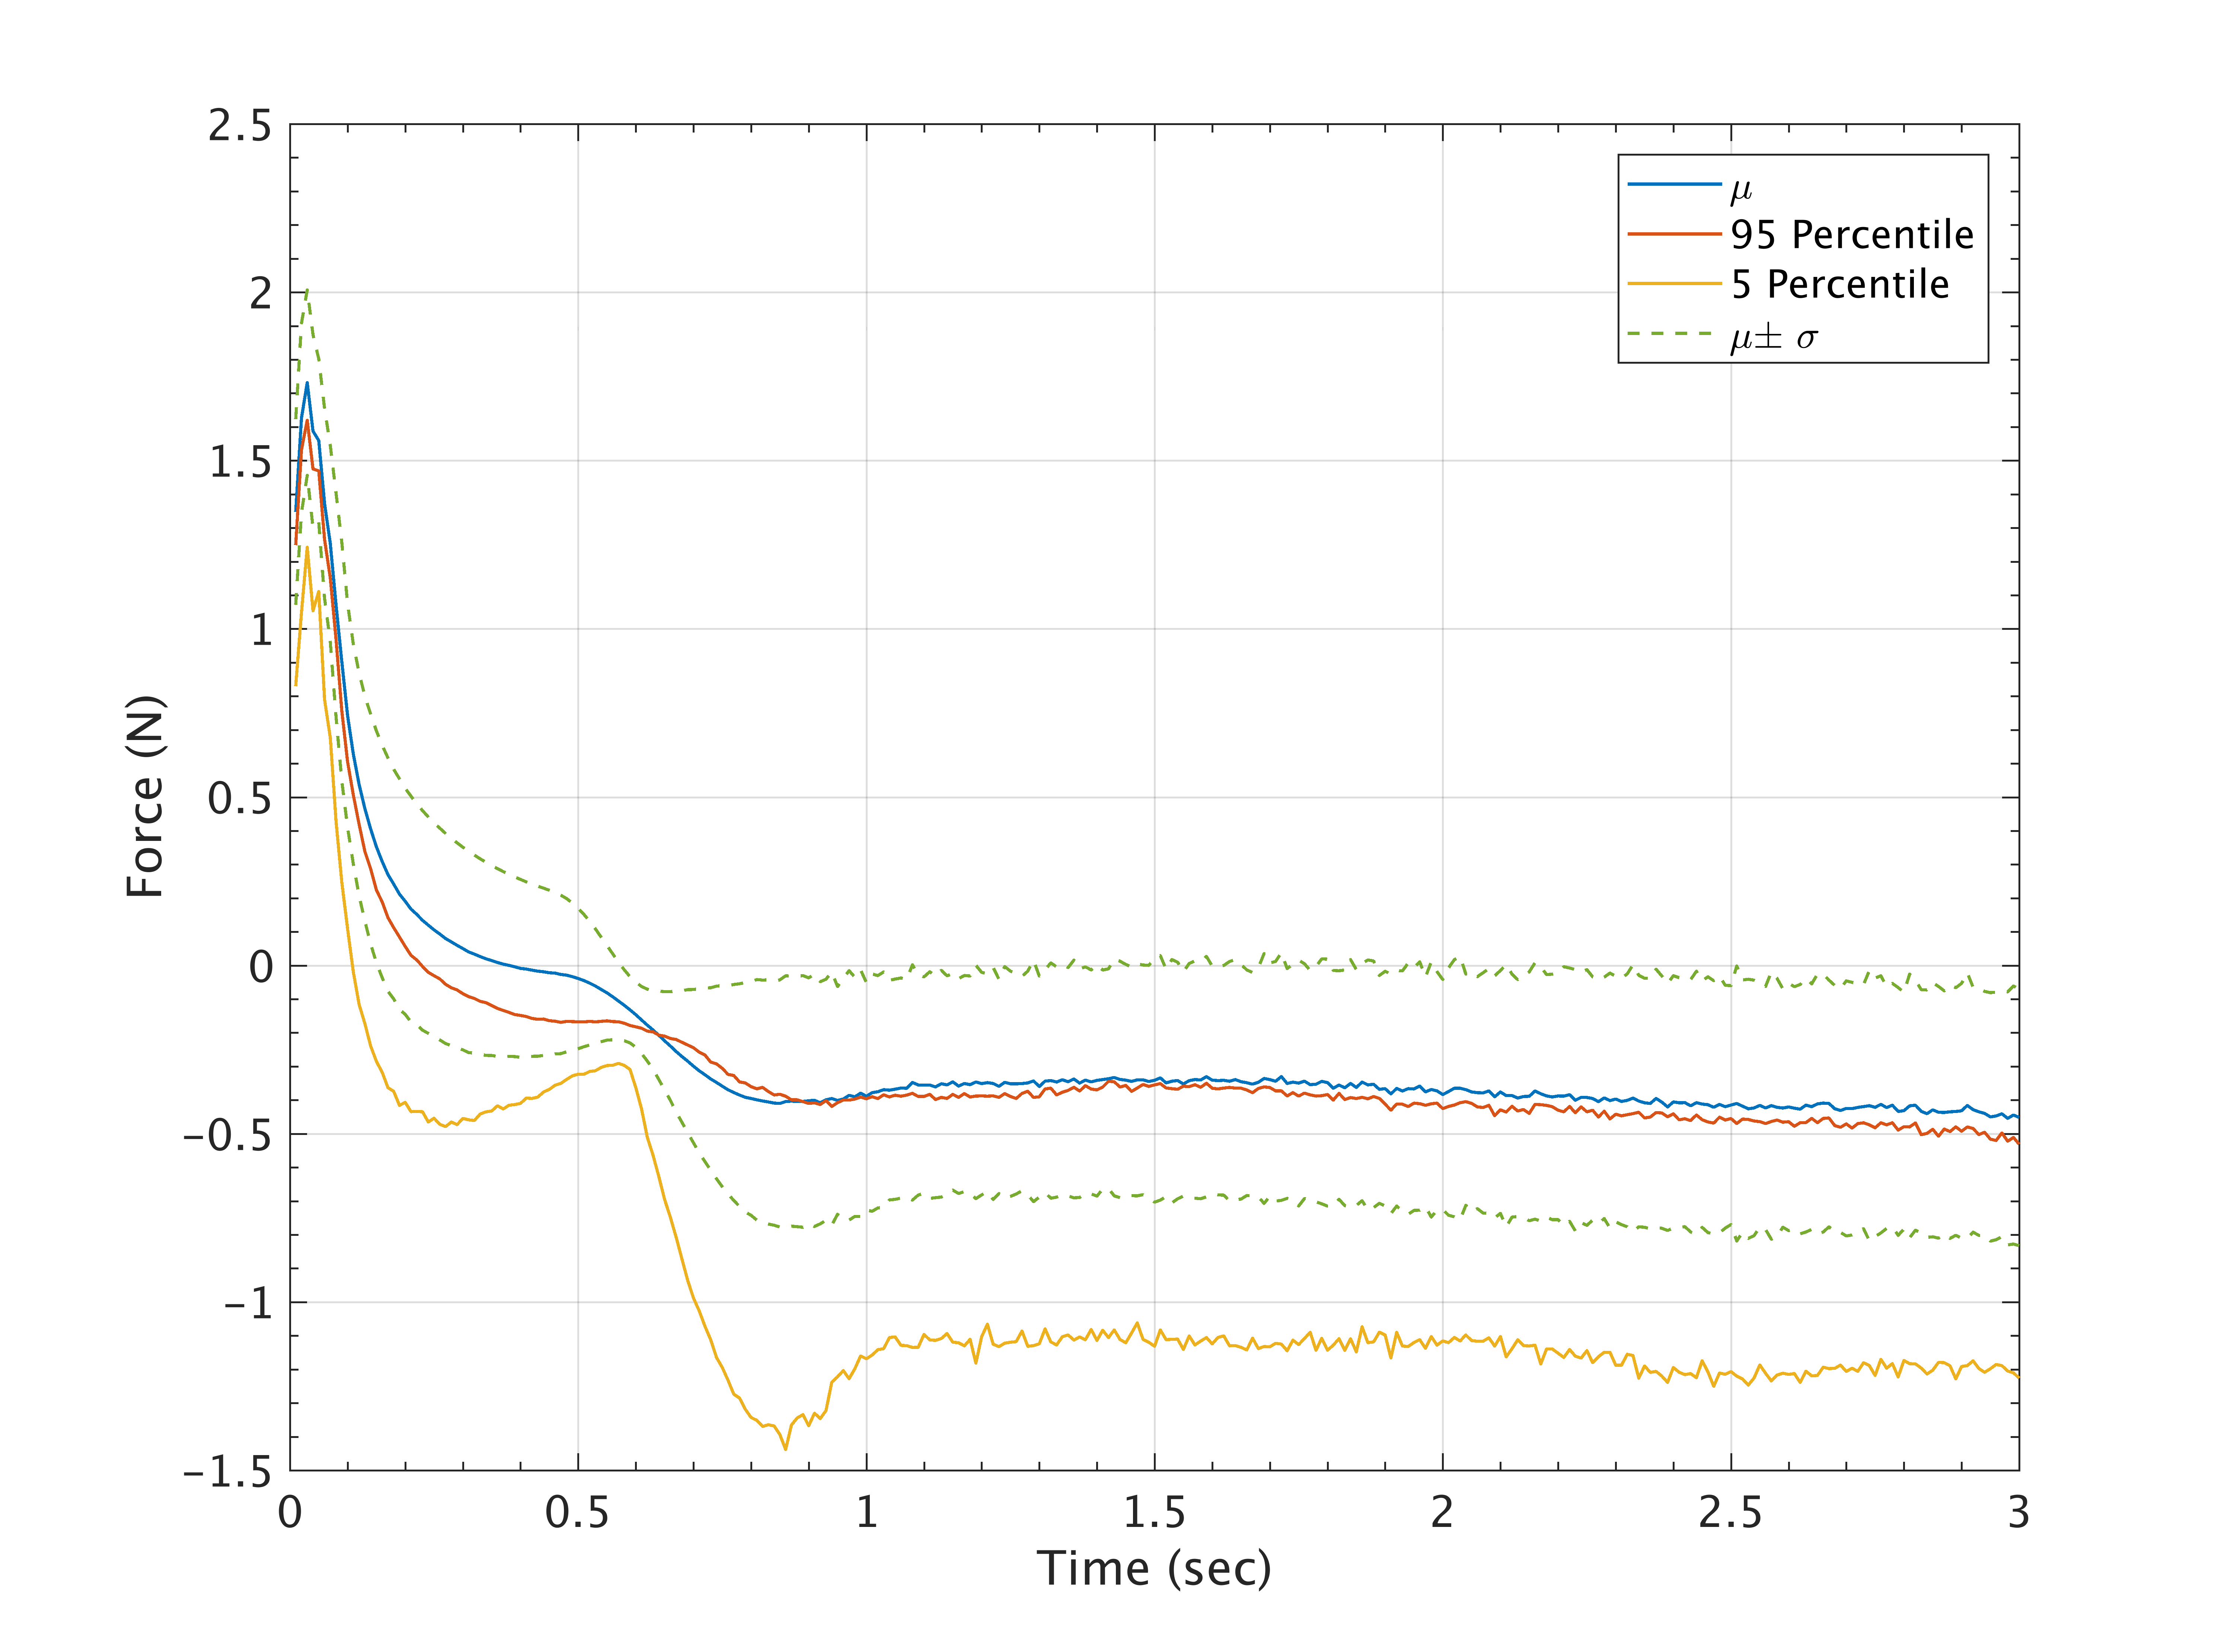
\includegraphics[width=1\textwidth]{InclinedPlane/GlobalRecords/P_Global_Fx.png}
                \subcaption{Pouliquen-Forterre model, runout direction.}
                \label{fig:Ramp-SP-Fx-P}
        \end{minipage}
        \begin{minipage}[b]{0.5\linewidth}
                \centering
                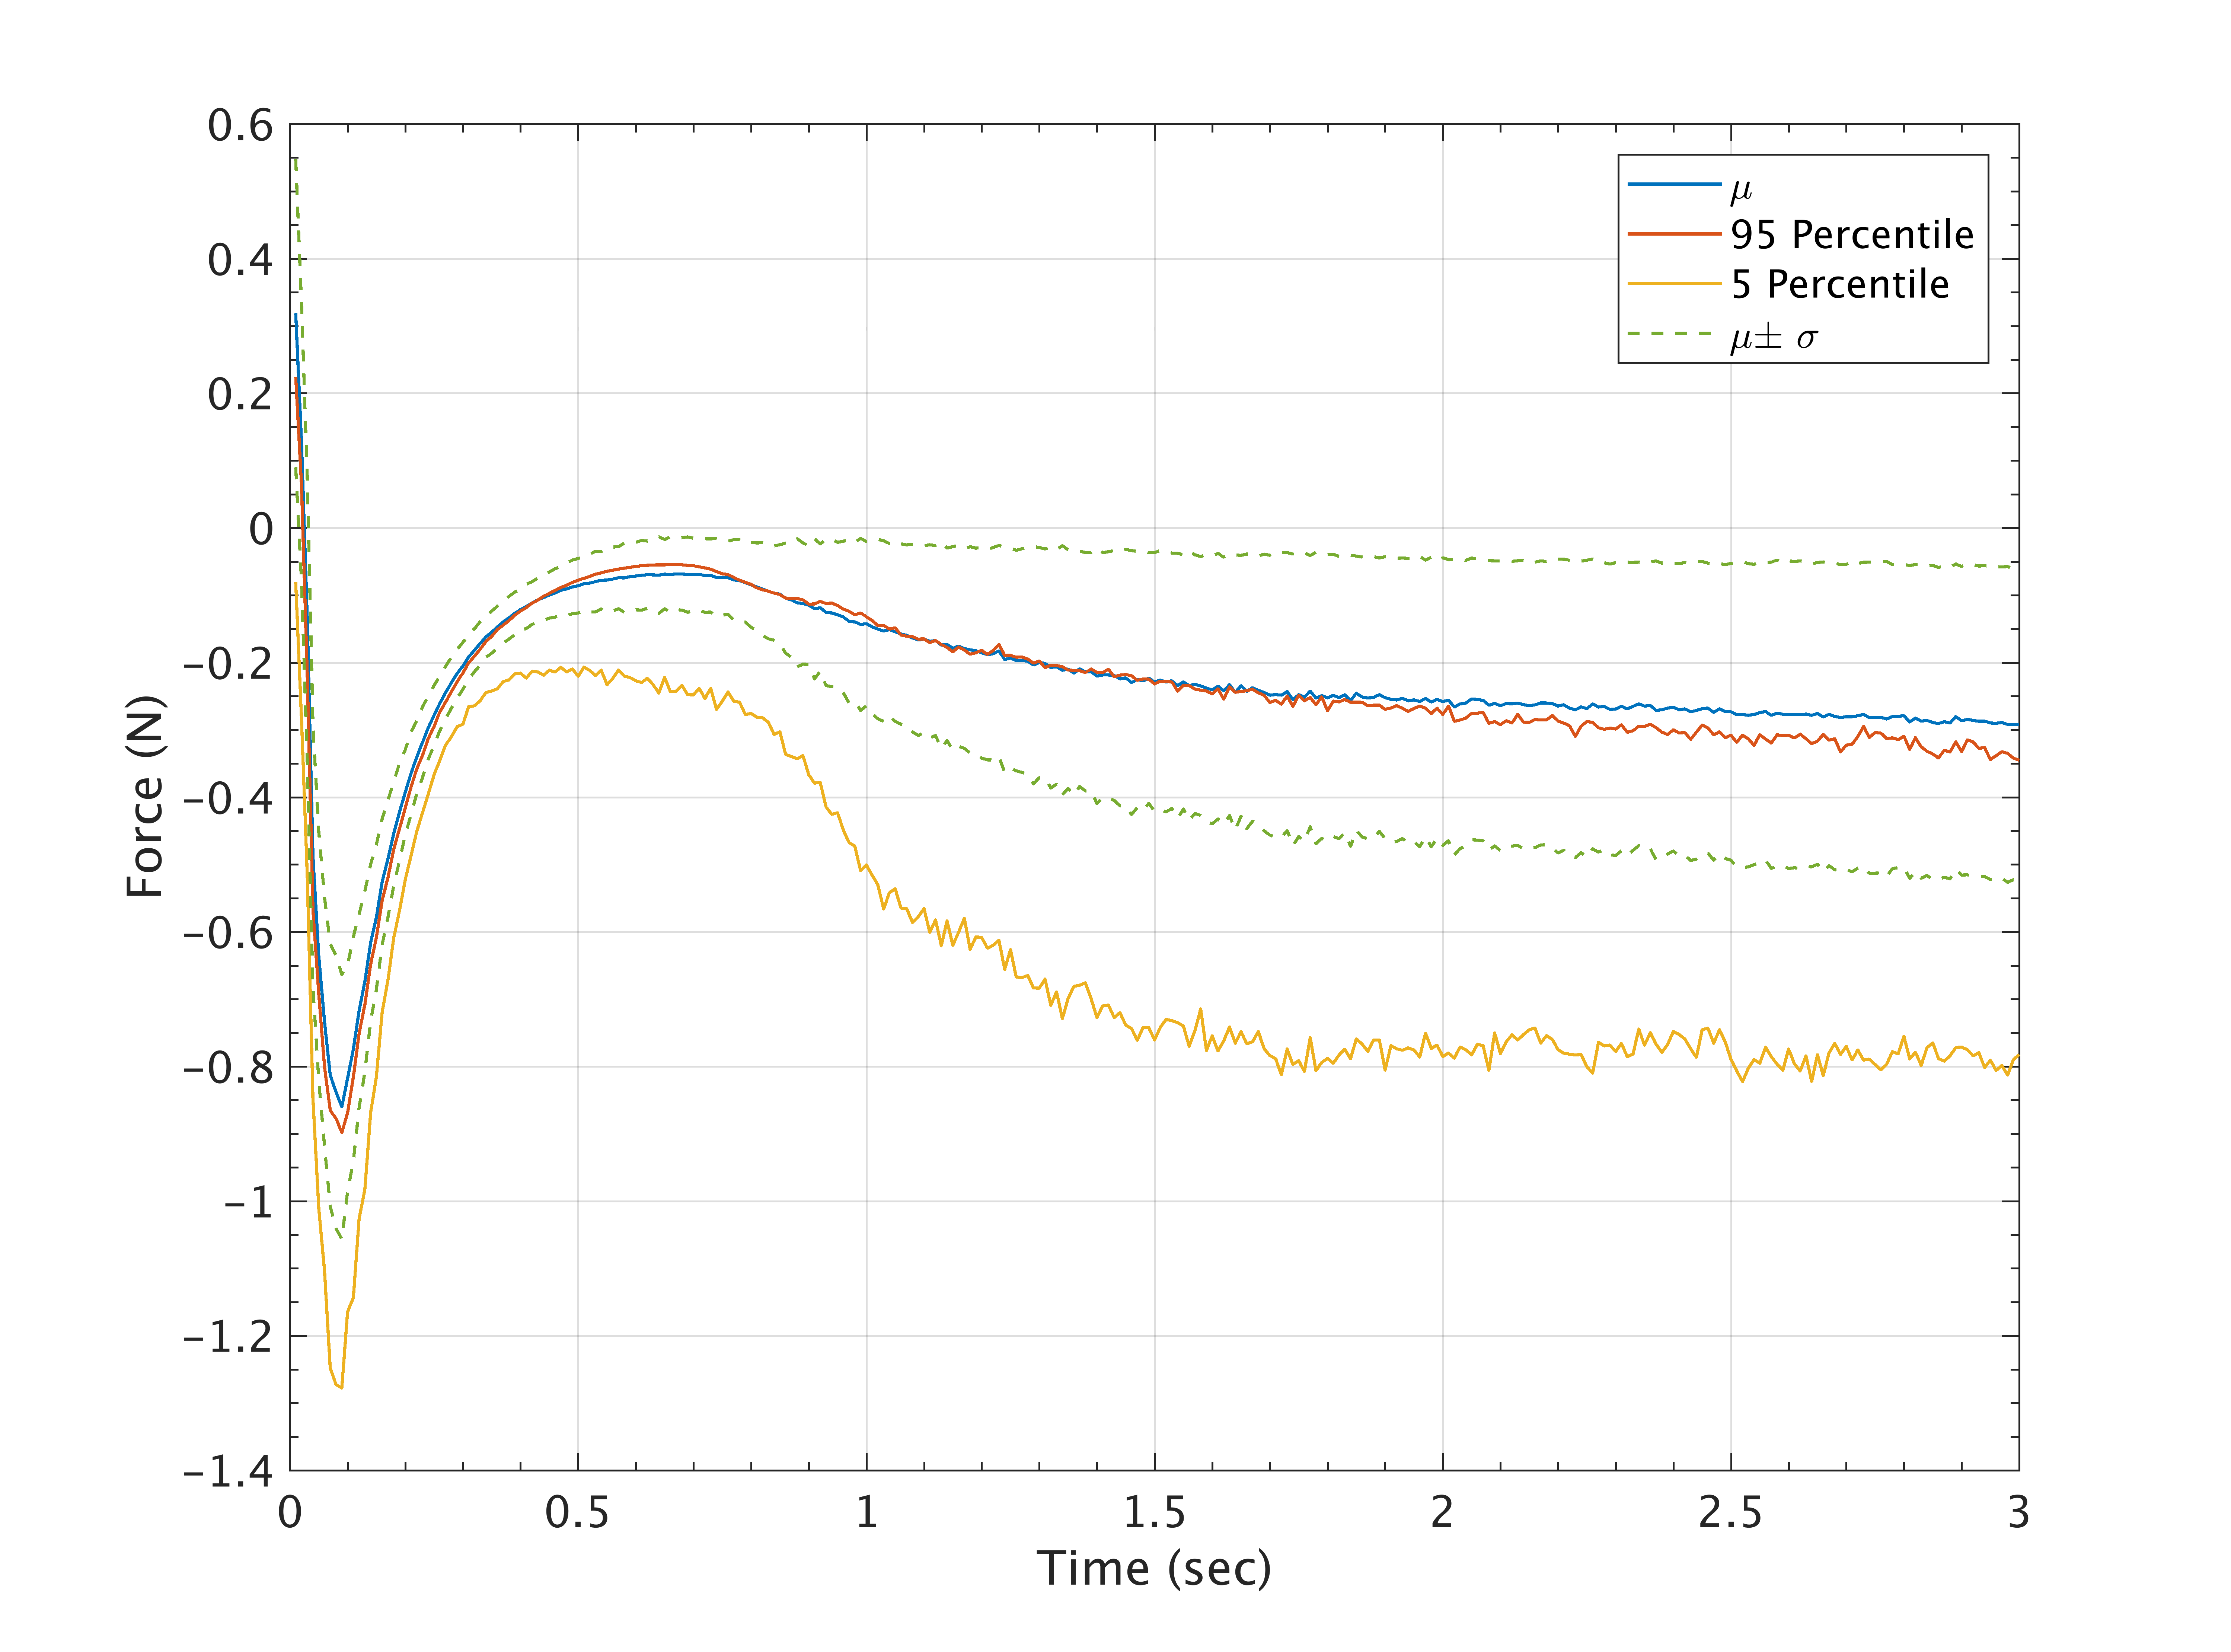
\includegraphics[width=1\textwidth]{InclinedPlane/GlobalRecords/P_Global_Fy.png}
                \subcaption{Pouliquen-Forterre model, lateral direction.}
                \label{fig:Ramp-SP-Fy-P}
        \end{minipage}

        \begin{minipage}[b]{0.5\linewidth}
                \centering
                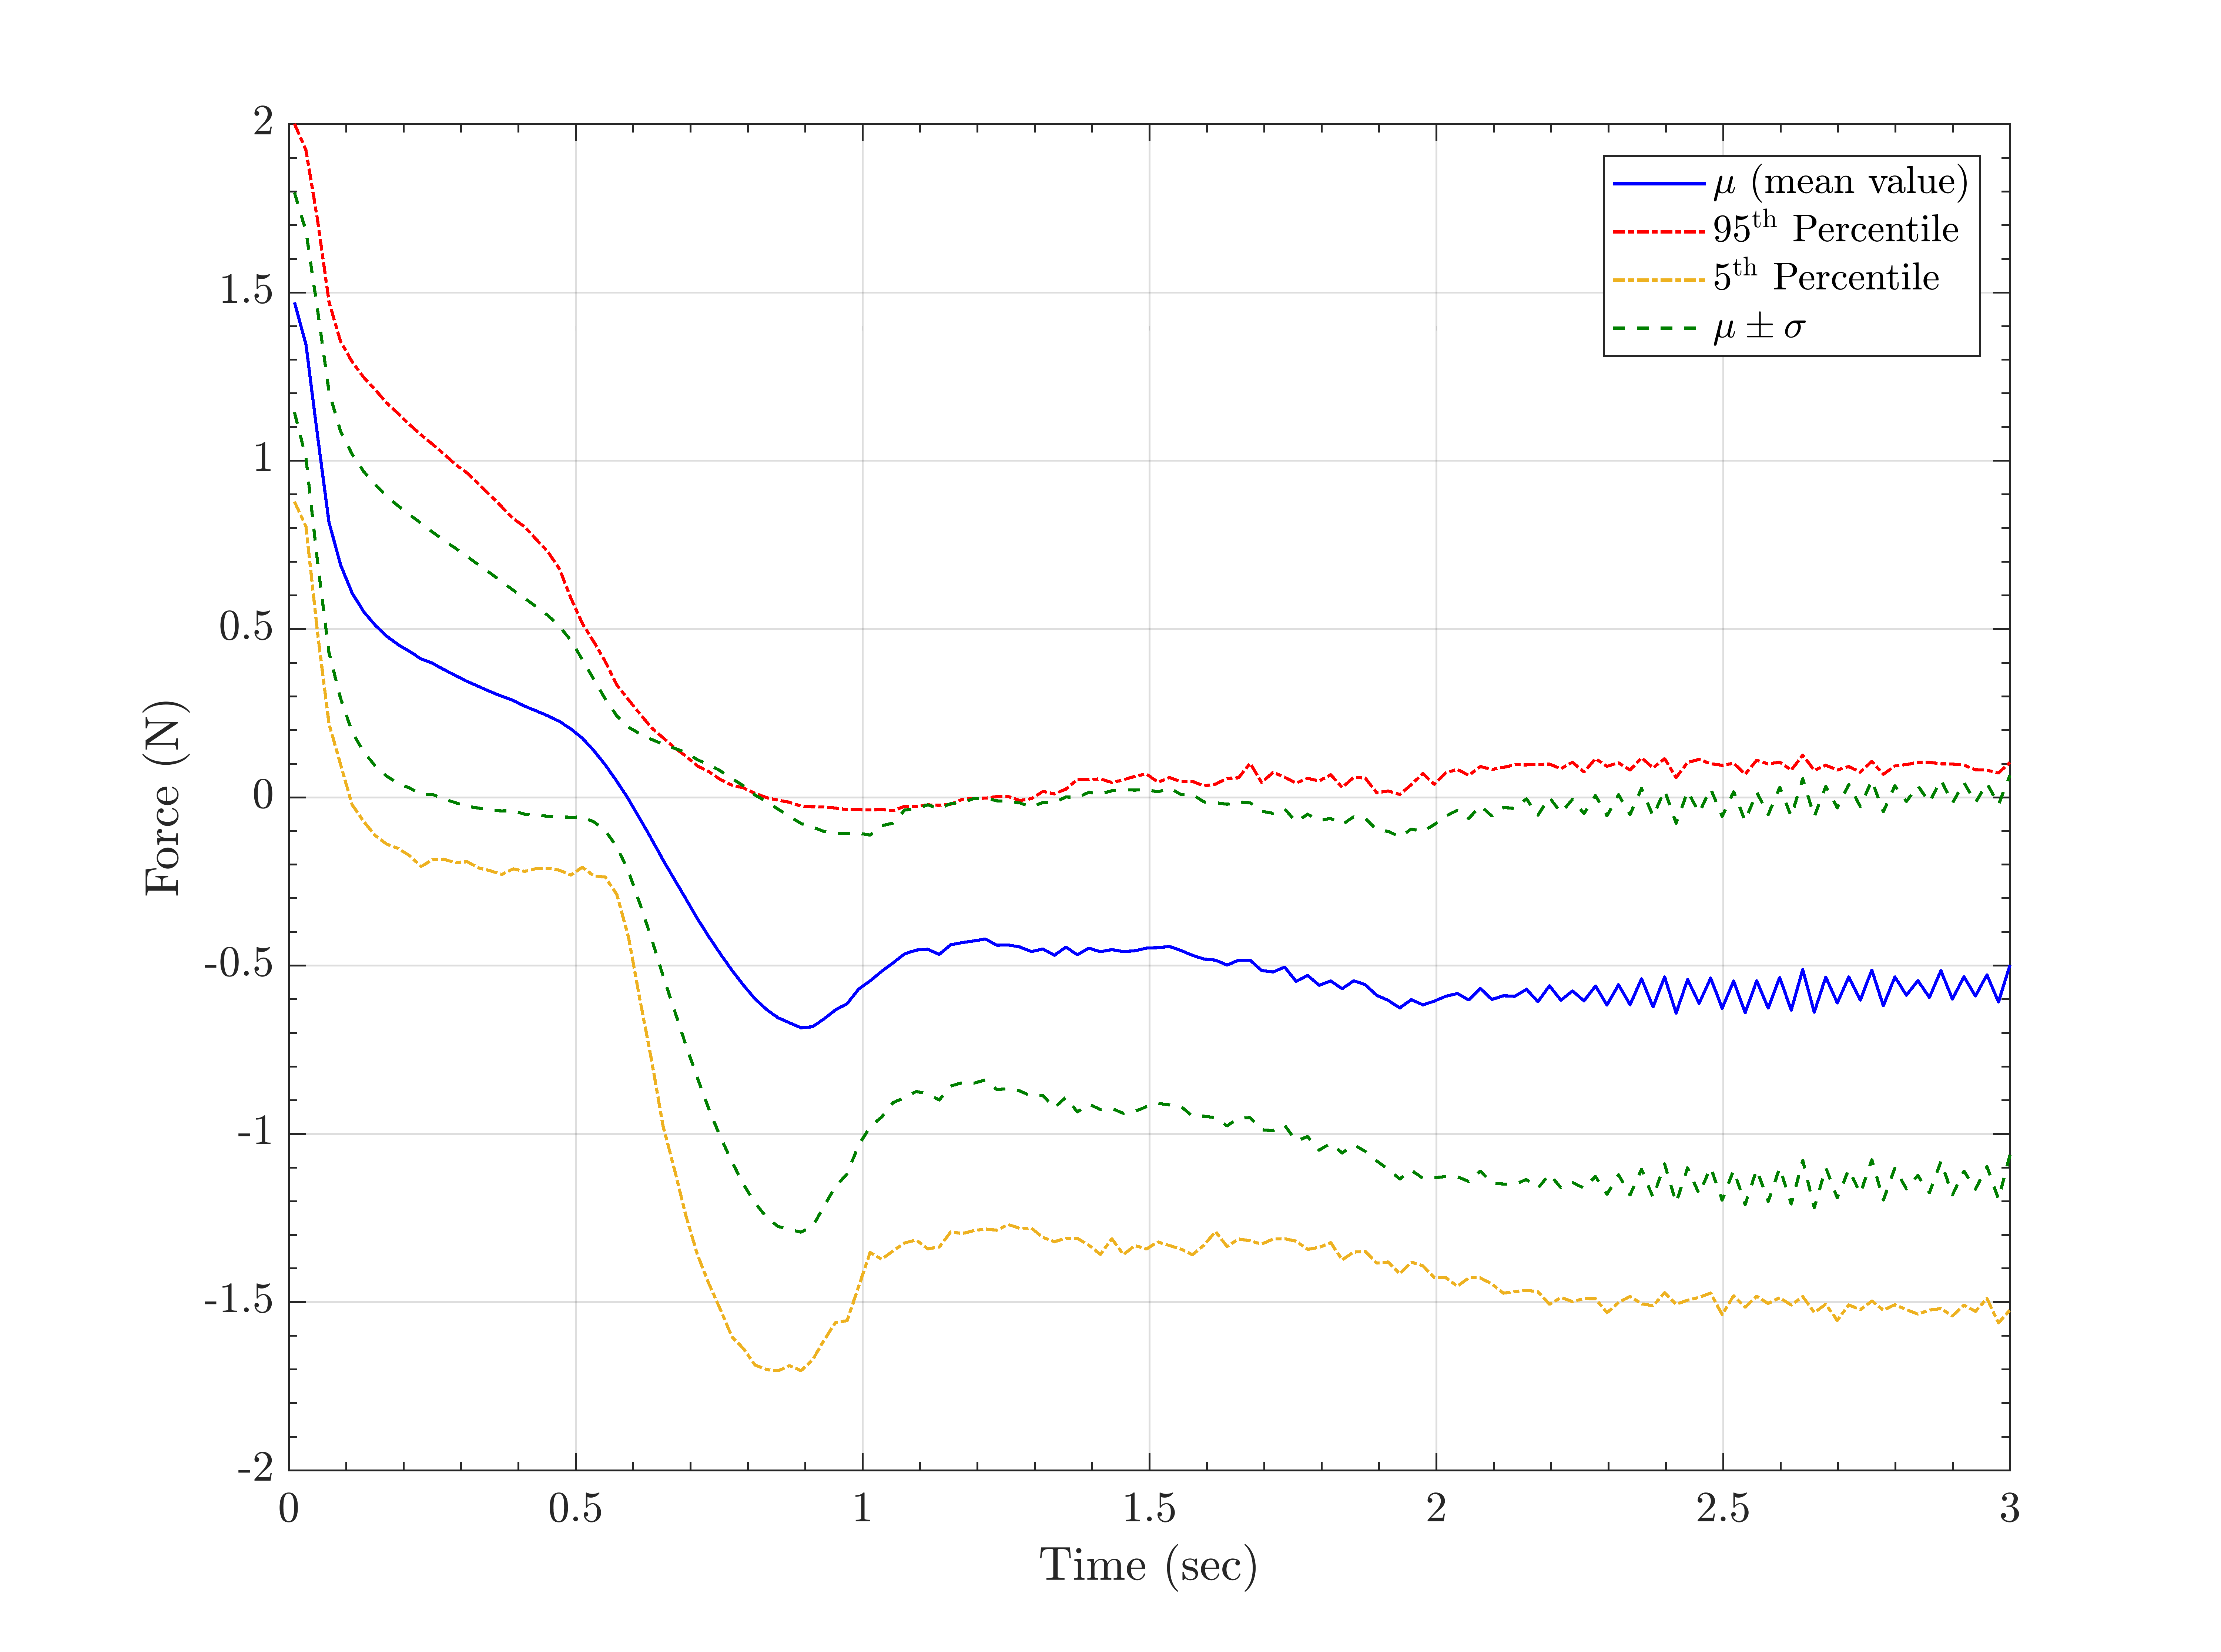
\includegraphics[width=1\textwidth]{InclinedPlane/GlobalRecords/V_Global_Fx.png}
                \subcaption{Voellmy-Salm model, runout direction.}
                \label{fig:Ramp-SP-Fx-V}
        \end{minipage}
        \begin{minipage}[b]{0.5\linewidth}
                \centering
                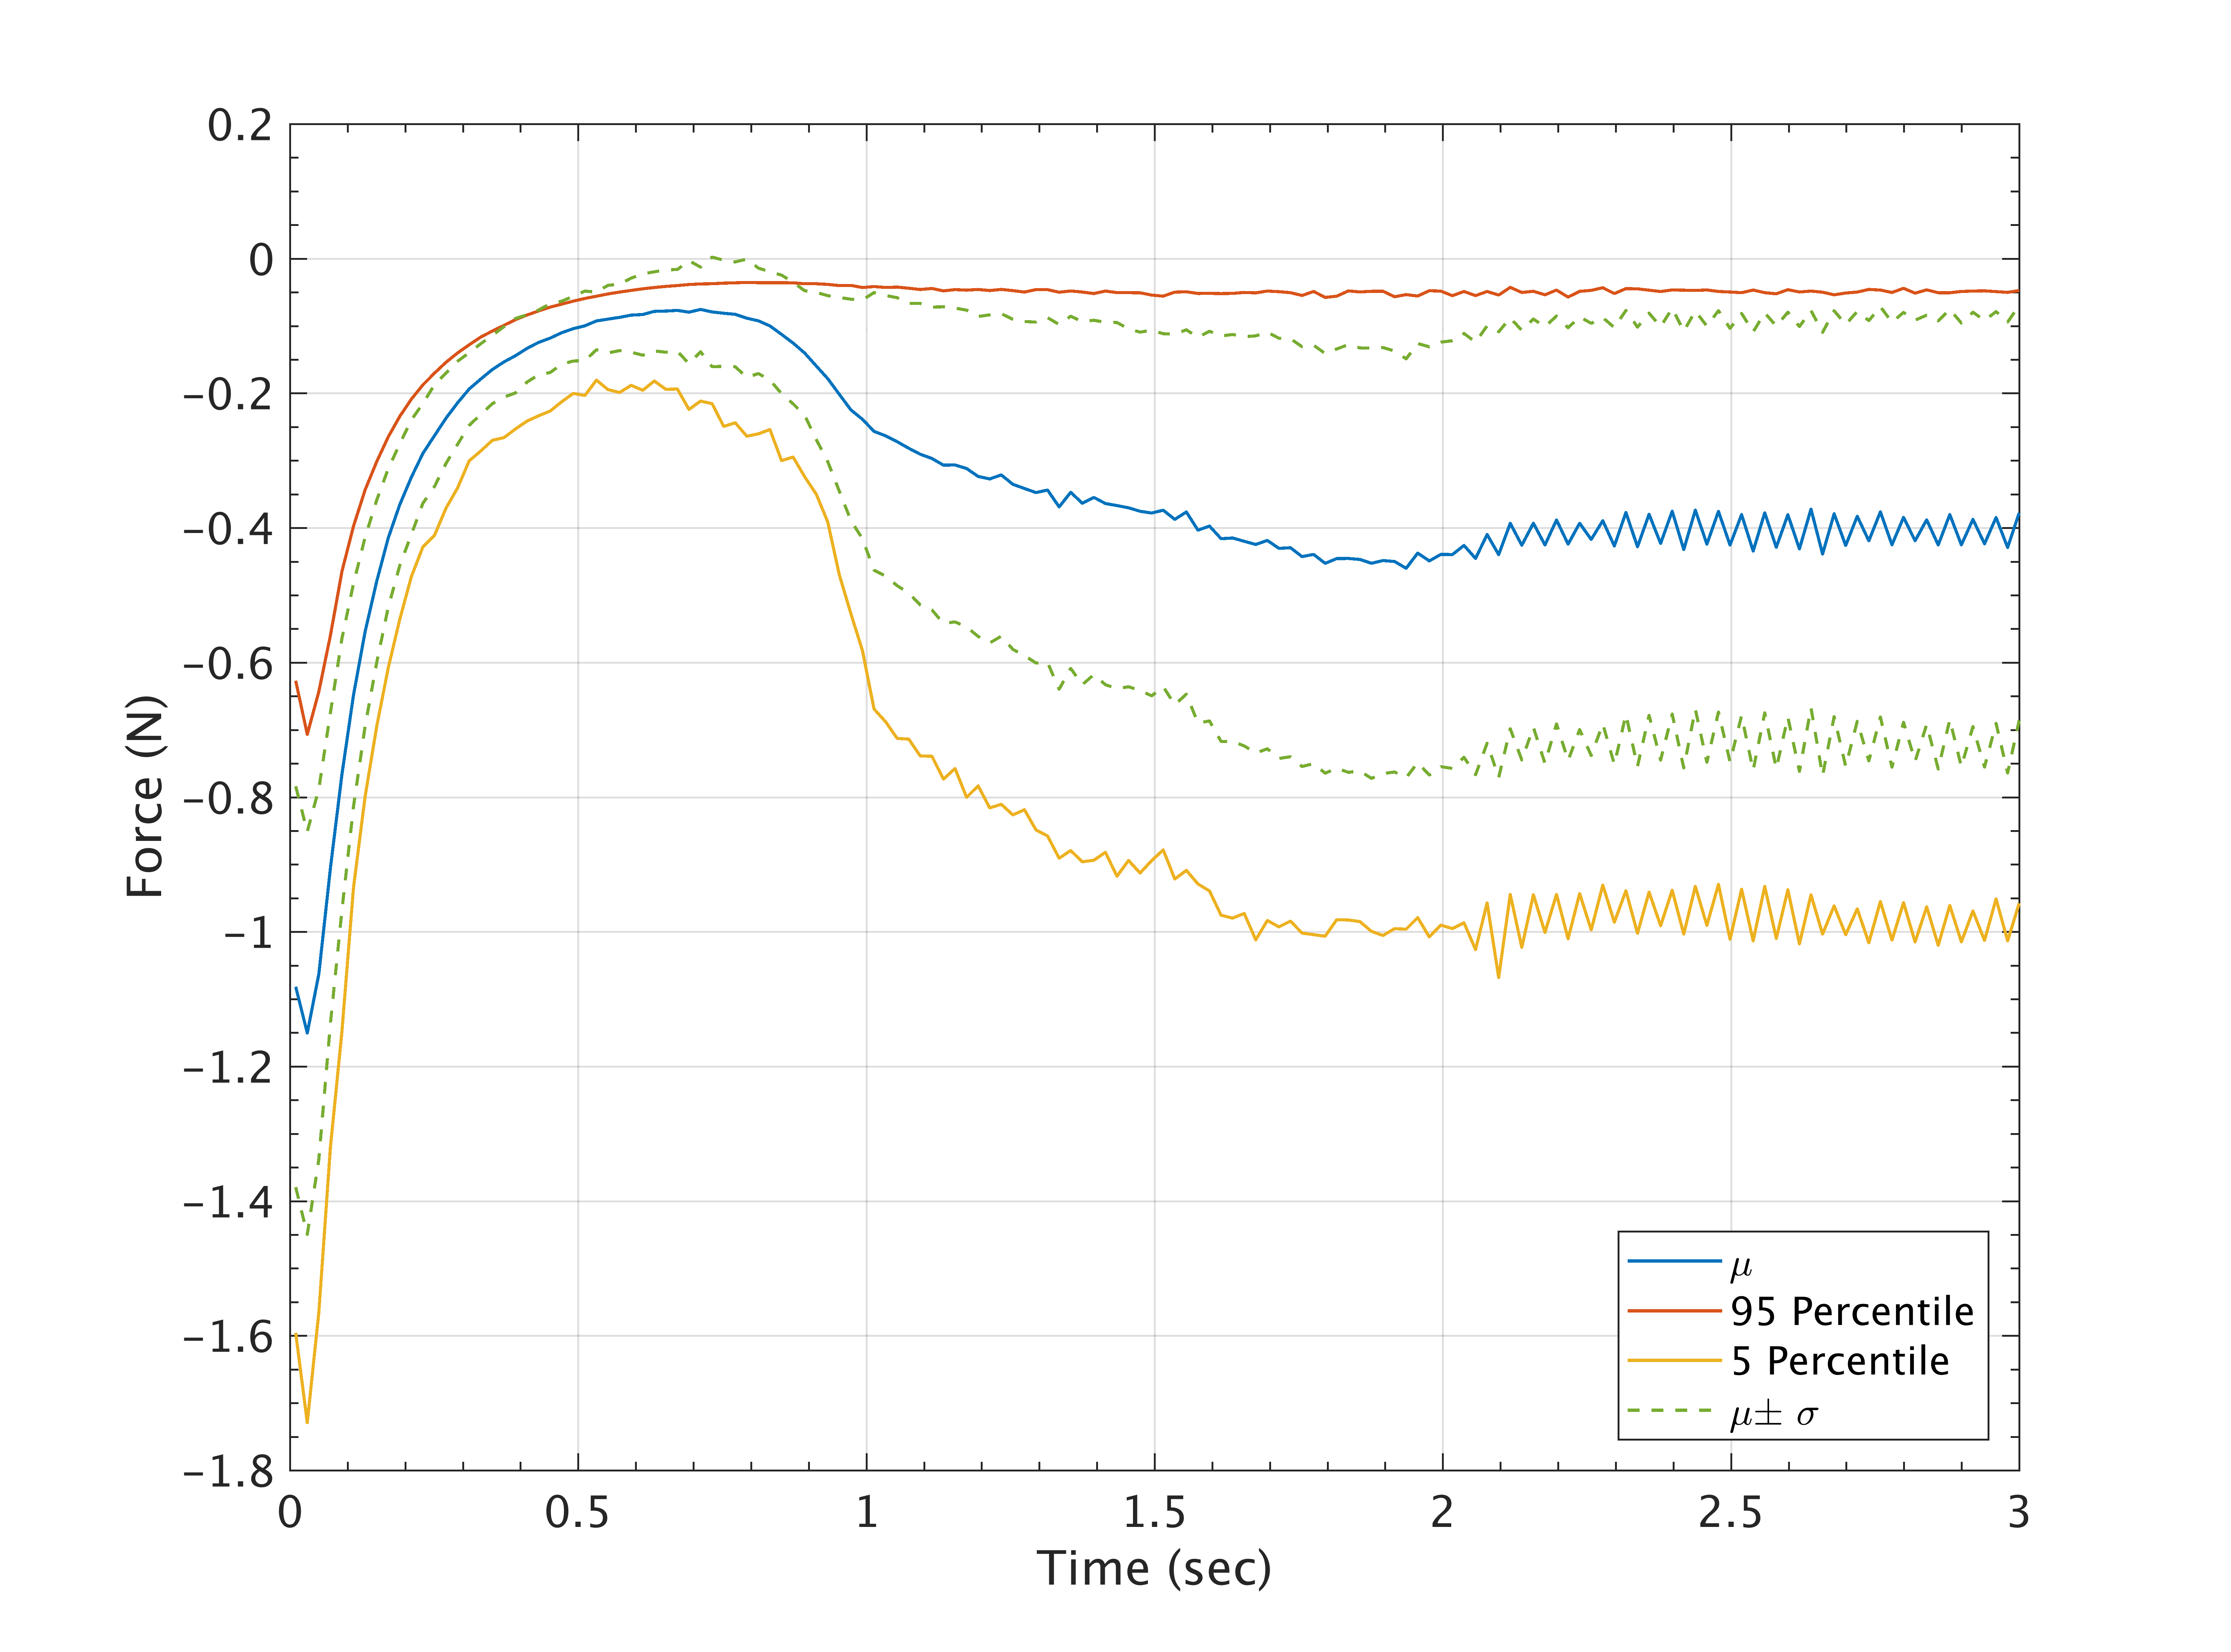
\includegraphics[width=1\textwidth]{InclinedPlane/GlobalRecords/V_Global_Fy.png}
                \subcaption{Voellmy-Salm model, lateral direction.}
                \label{fig:Ramp-SP-Fy-V}
        \end{minipage}
        \caption{Full statistics for temporal records of total forces for bulk of material along the runout and lateral directions.}
        \label{fig:Ramp-SP-F}
\end{figure}

\begin{figure}[H]
        \begin{minipage}[b]{0.5\linewidth}
                \centering
                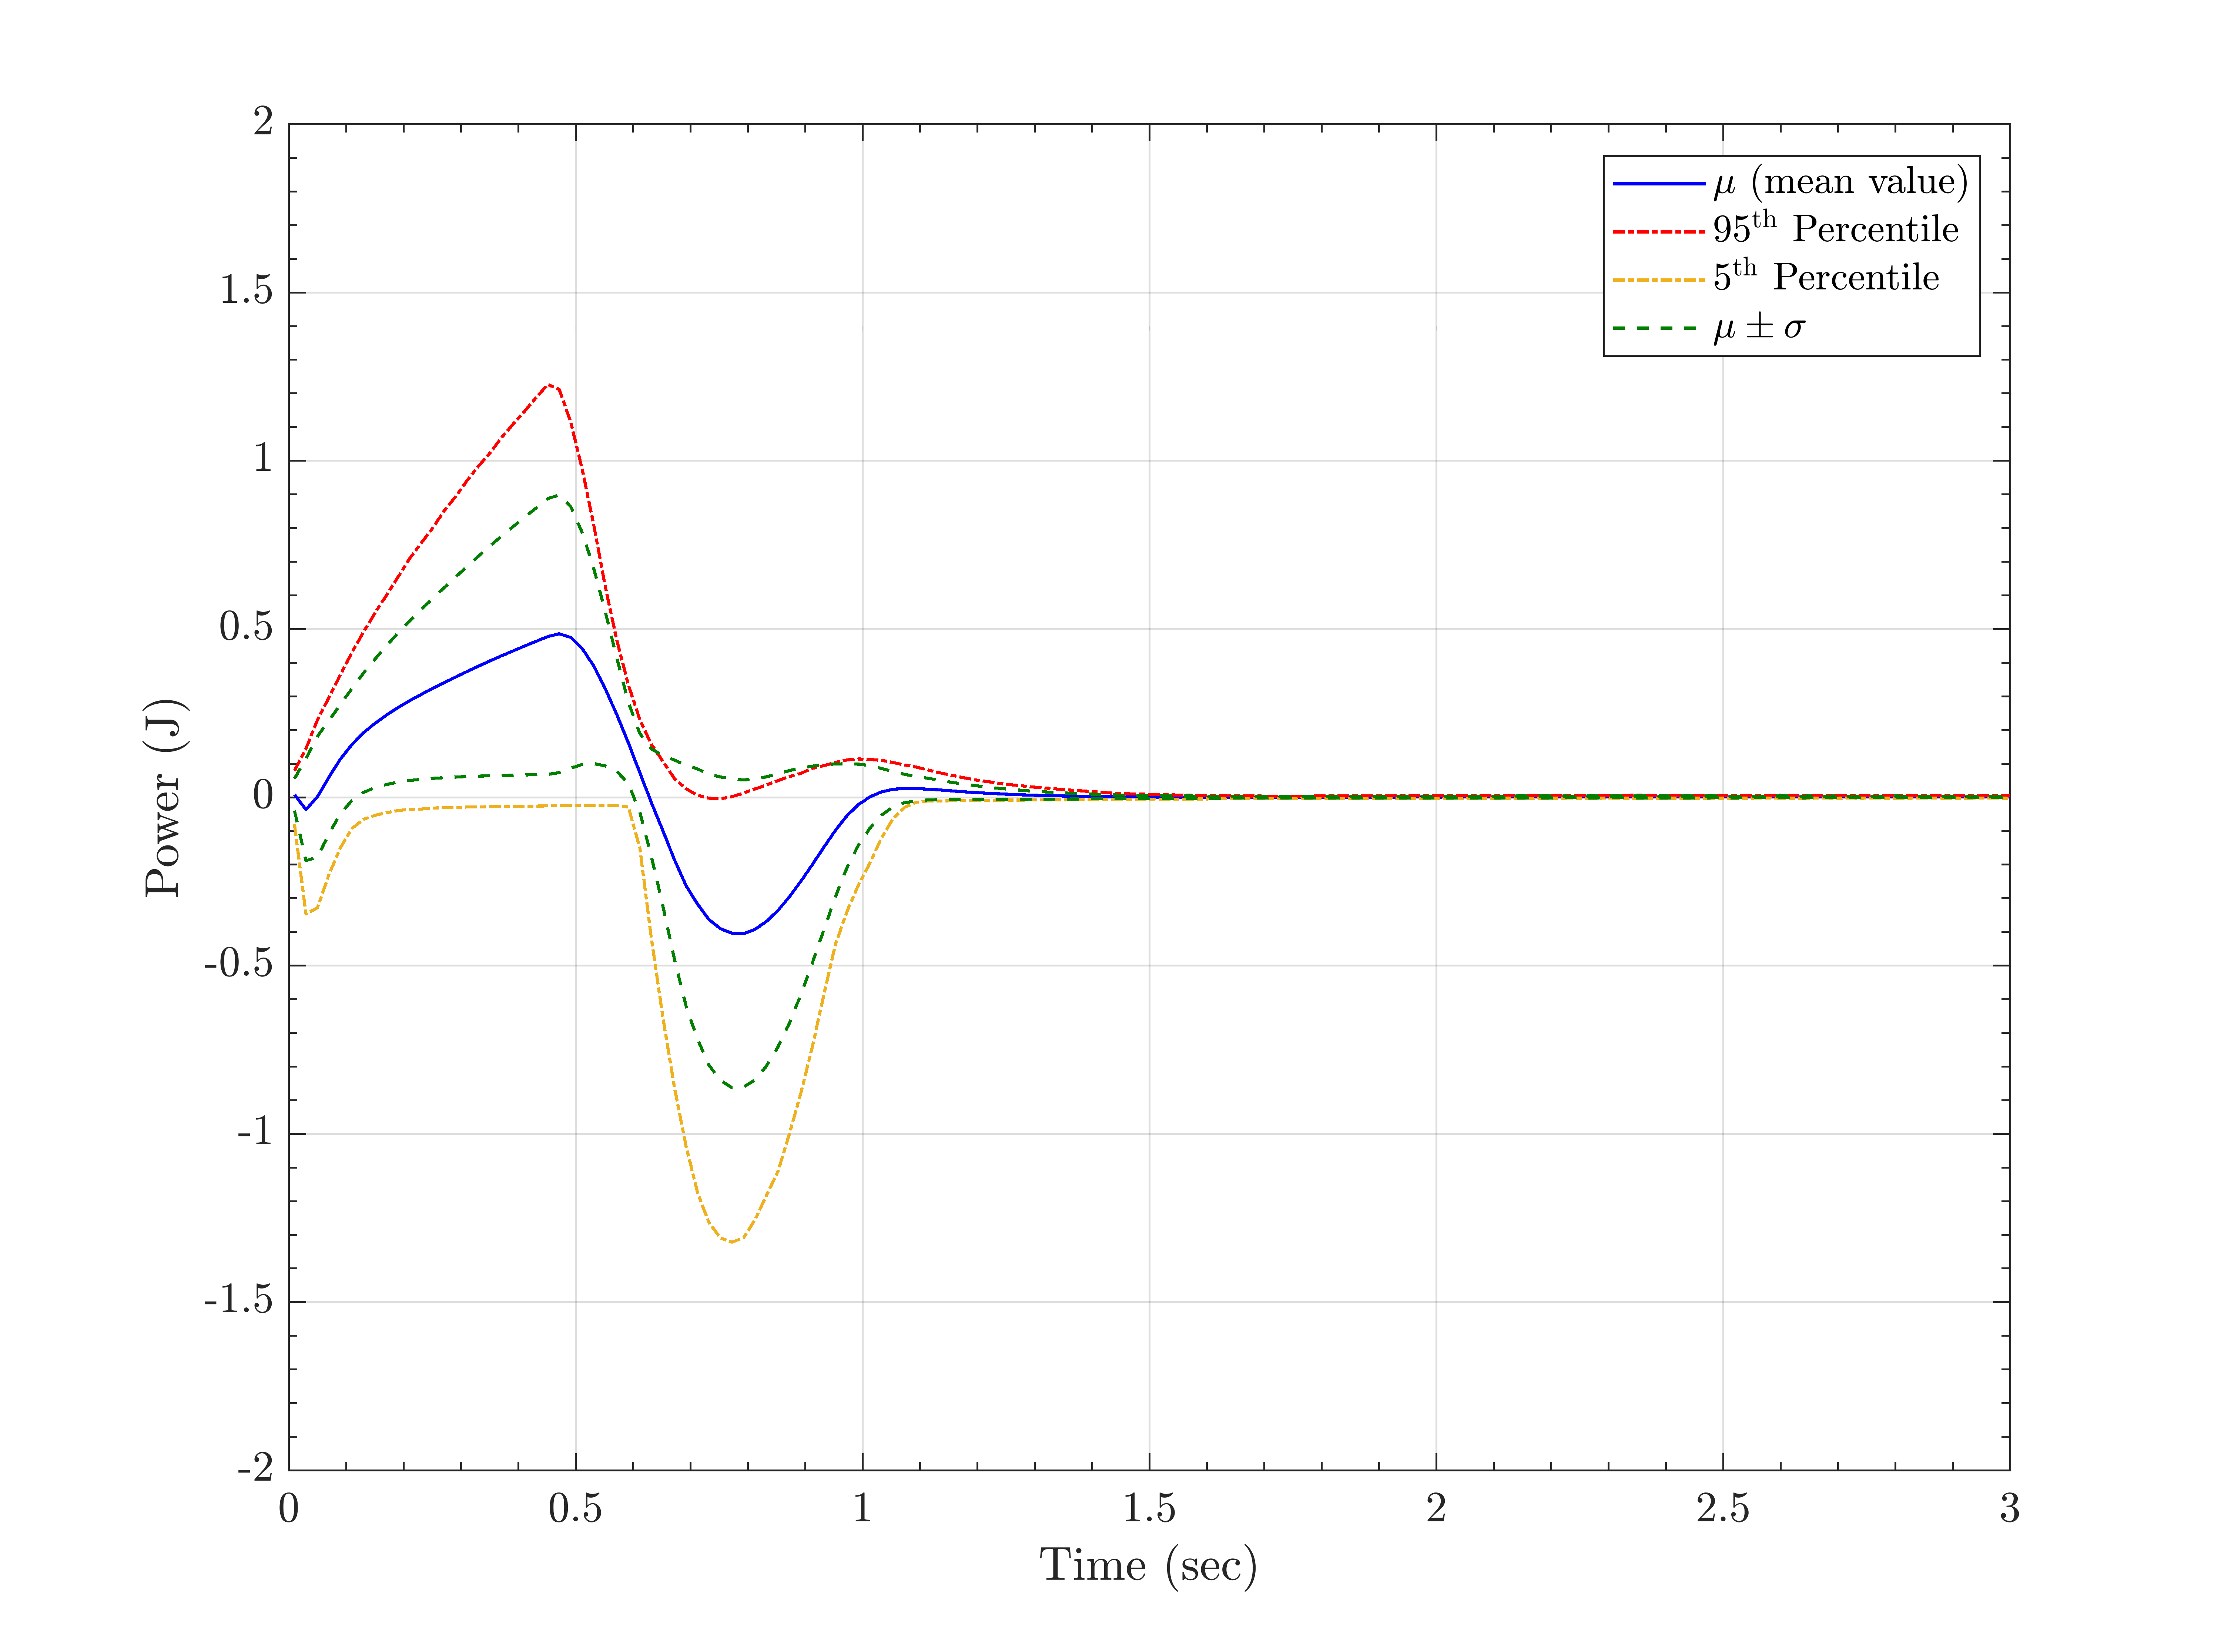
\includegraphics[width=1\textwidth]{InclinedPlane/GlobalRecords/C_Global_Ptot.png}
                \subcaption{Mohr-Coulomb model.}
                \label{fig:Ramp-SP-Power-C}
        \end{minipage}
        \begin{minipage}[b]{0.5\linewidth}
                \centering
                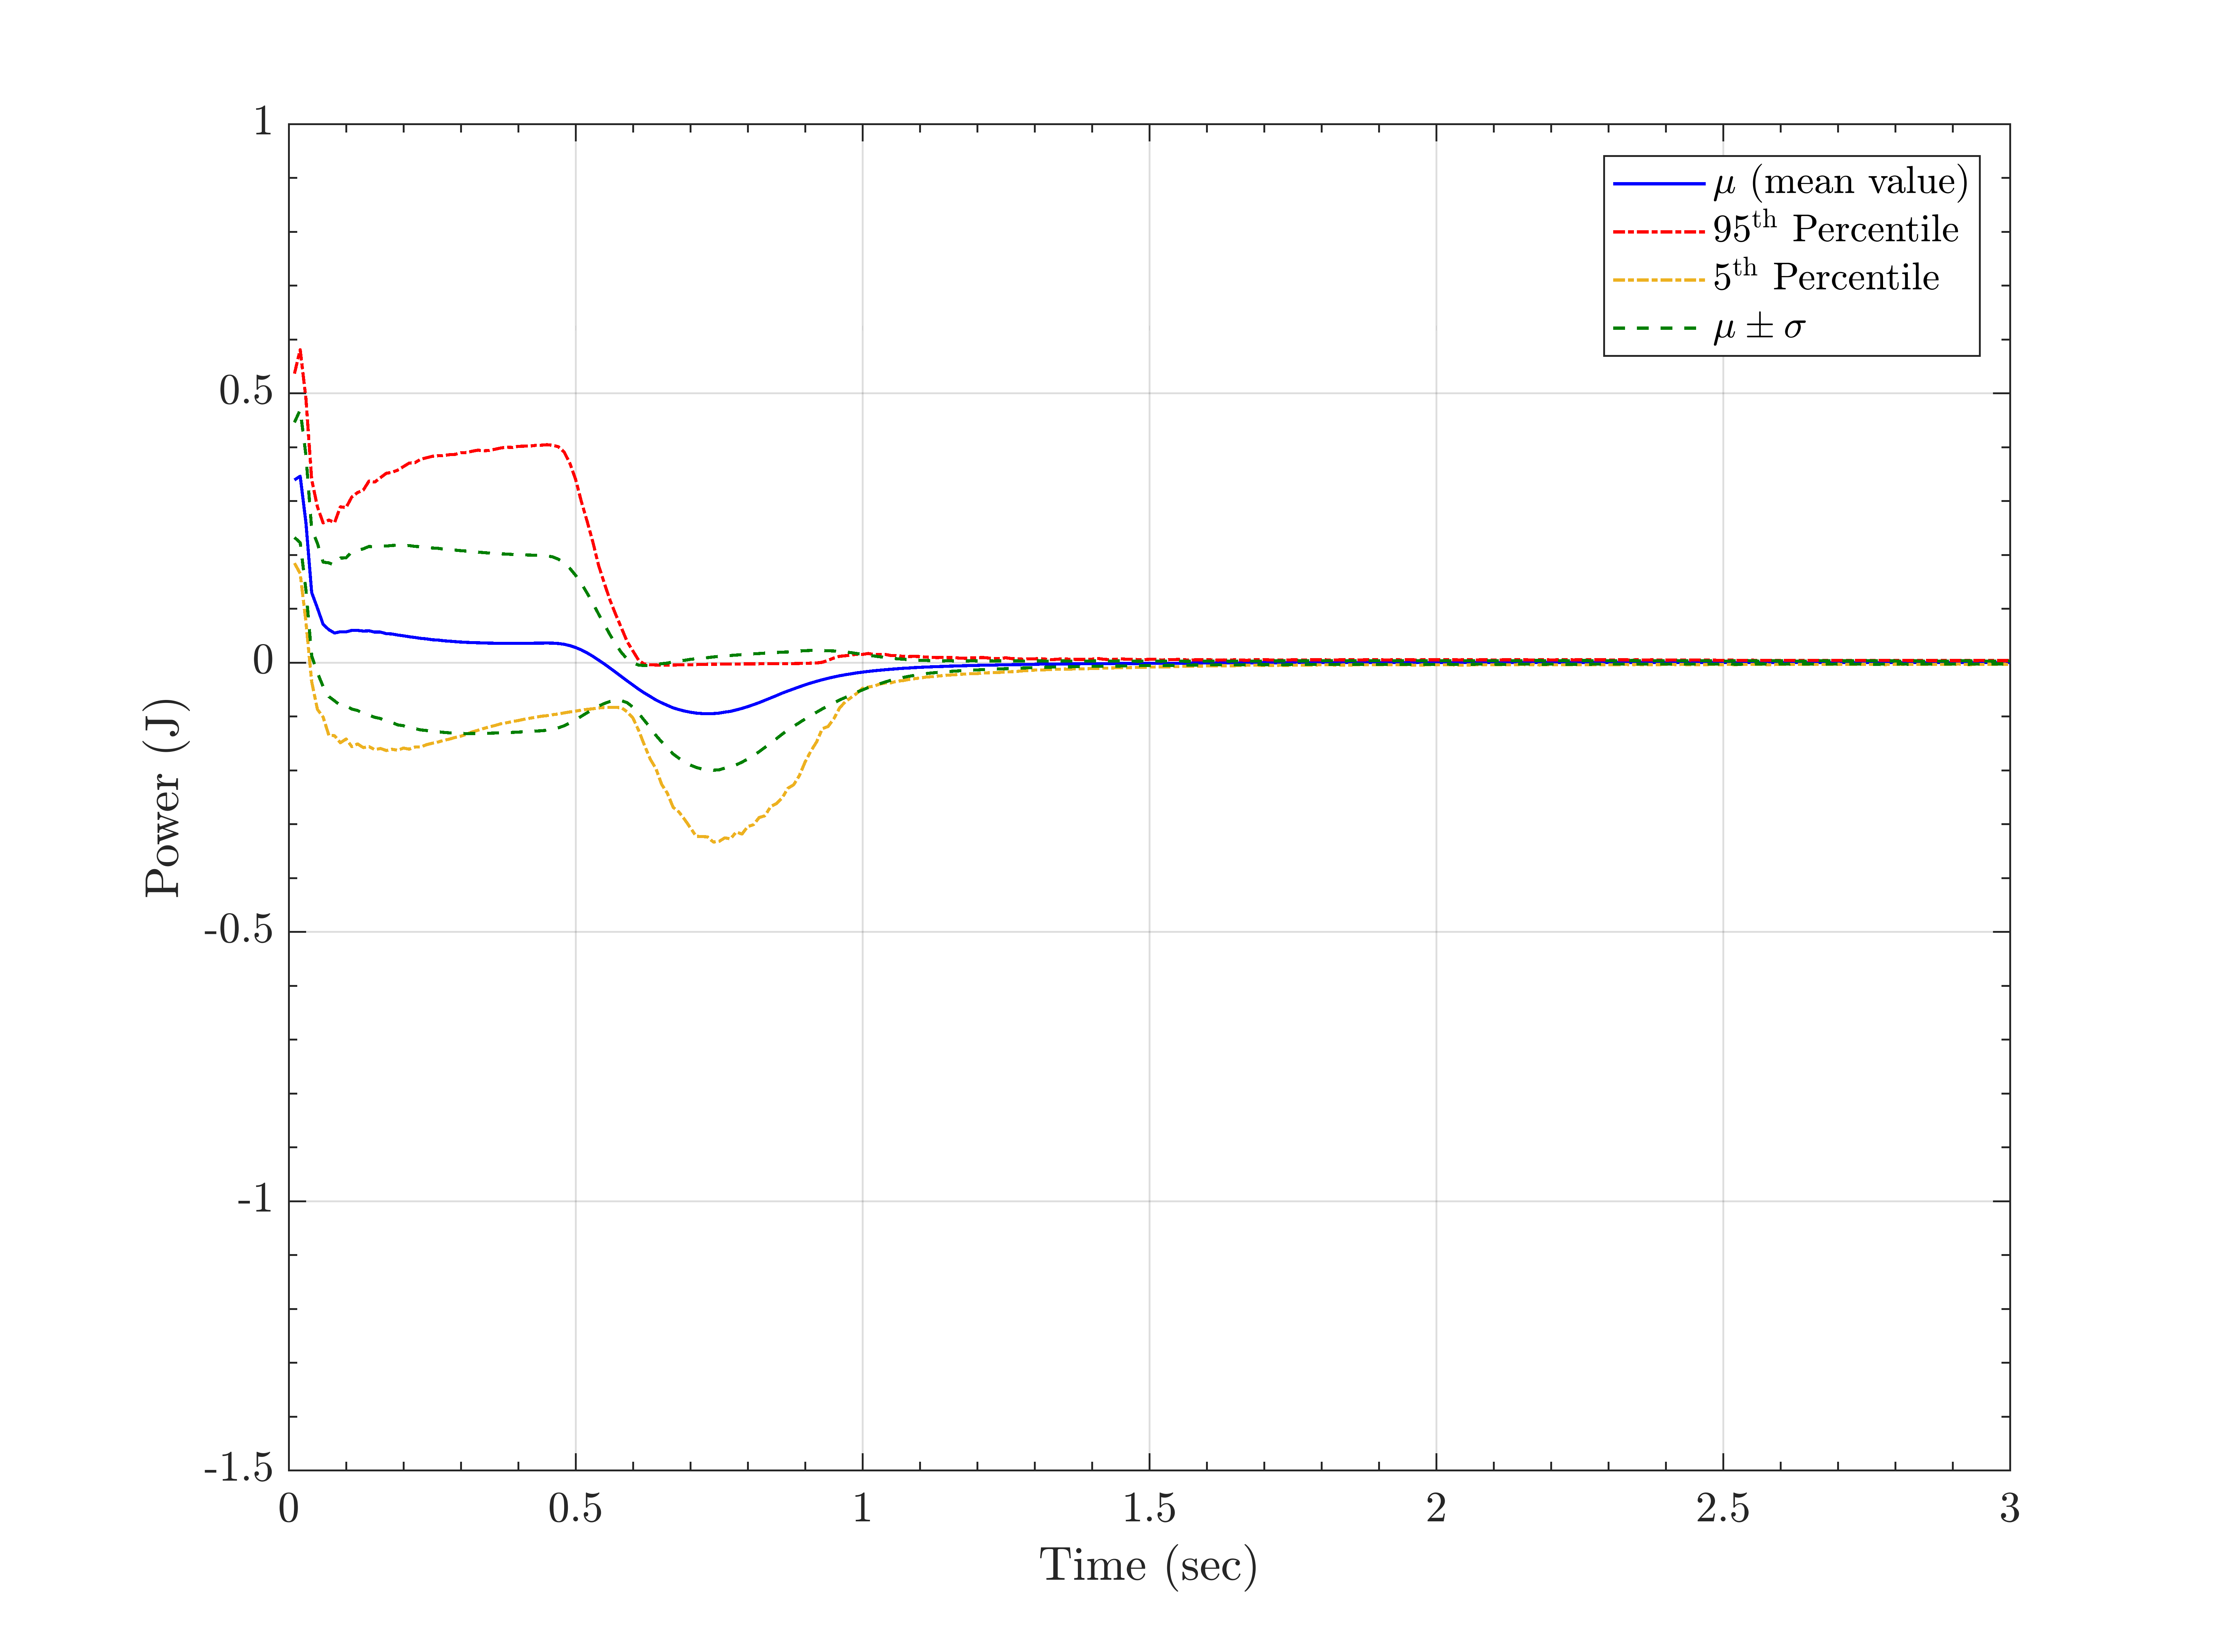
\includegraphics[width=1\textwidth]{InclinedPlane/GlobalRecords/P_Global_Ptot.png}
                \subcaption{Pouliquen-Forterre model.}
                \label{fig:Ramp-SP-Power-P}
        \end{minipage}

        \begin{minipage}[b]{1\linewidth}
                \centering
                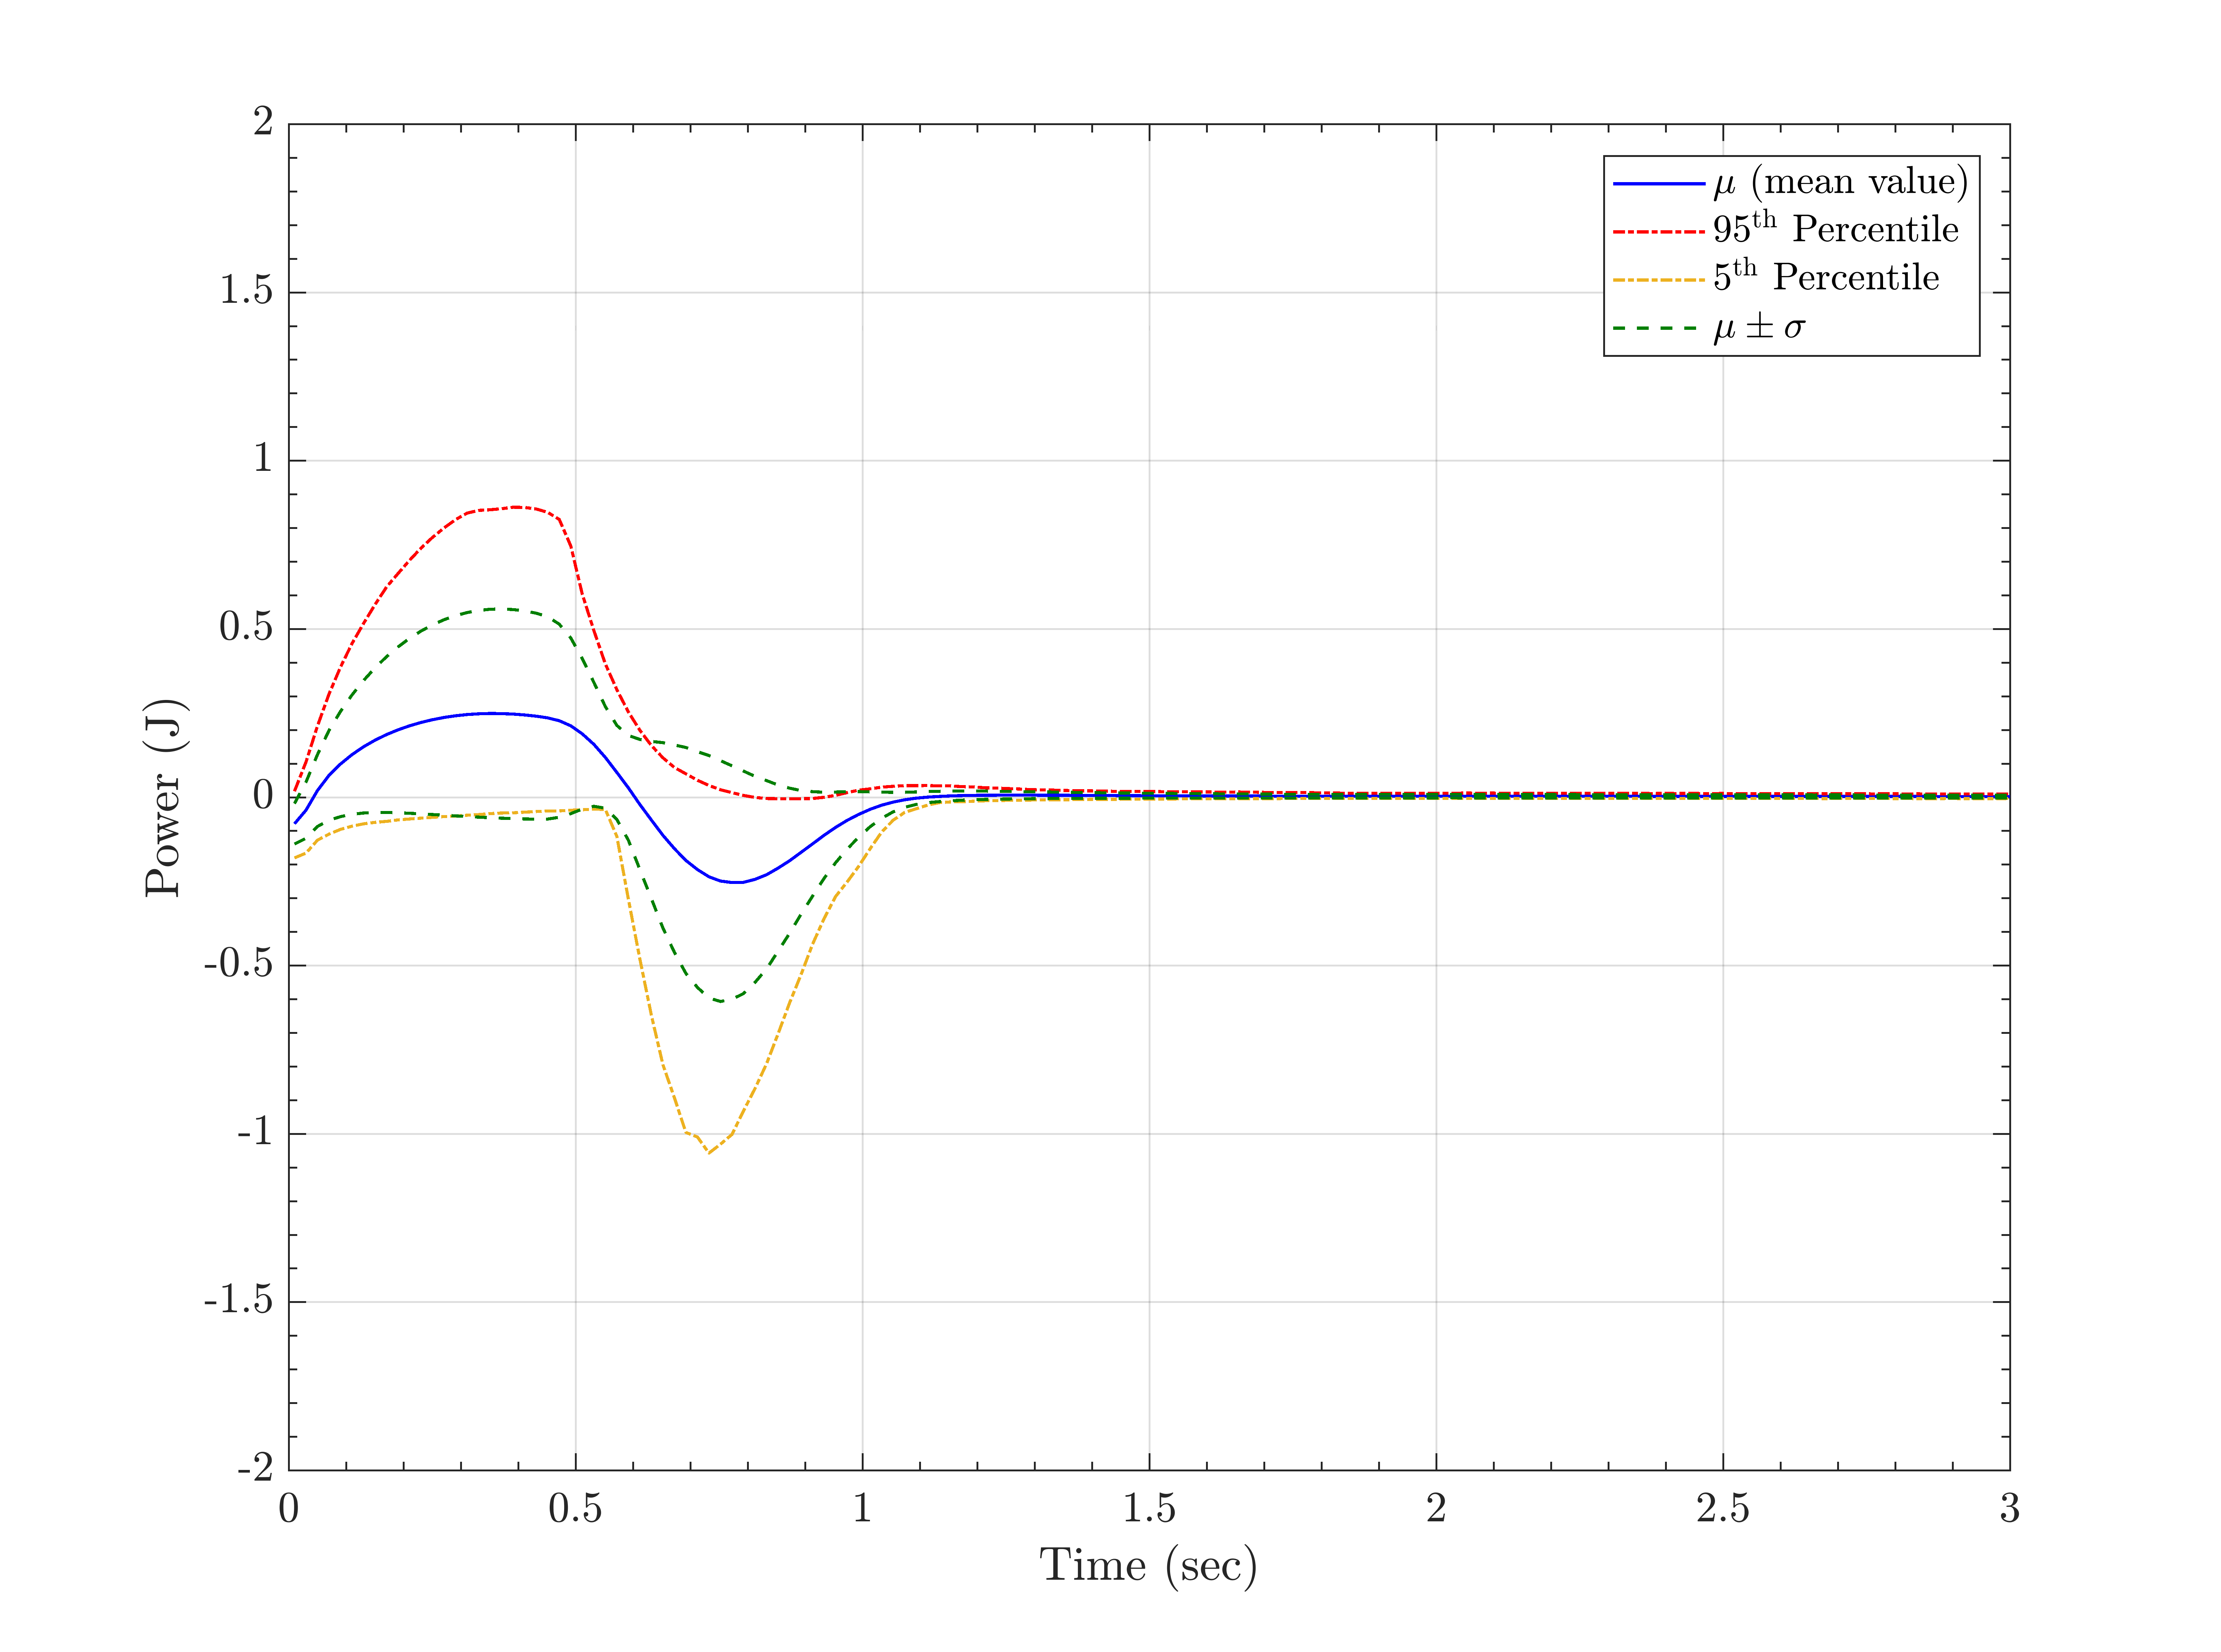
\includegraphics[width=0.5\textwidth]{InclinedPlane/GlobalRecords/V_Global_Ptot.png}
                \subcaption{Voellmy-Salm model.}
                \label{fig:Ramp-SP-Power-V}
        \end{minipage}
        \caption{Full statistics of temporal records of total power for bulk of material.}
        \label{fig:Ramp-SP-Power}
\end{figure}

\begin{figure}[H]
        \begin{minipage}[b]{0.5\linewidth}
                \centering
                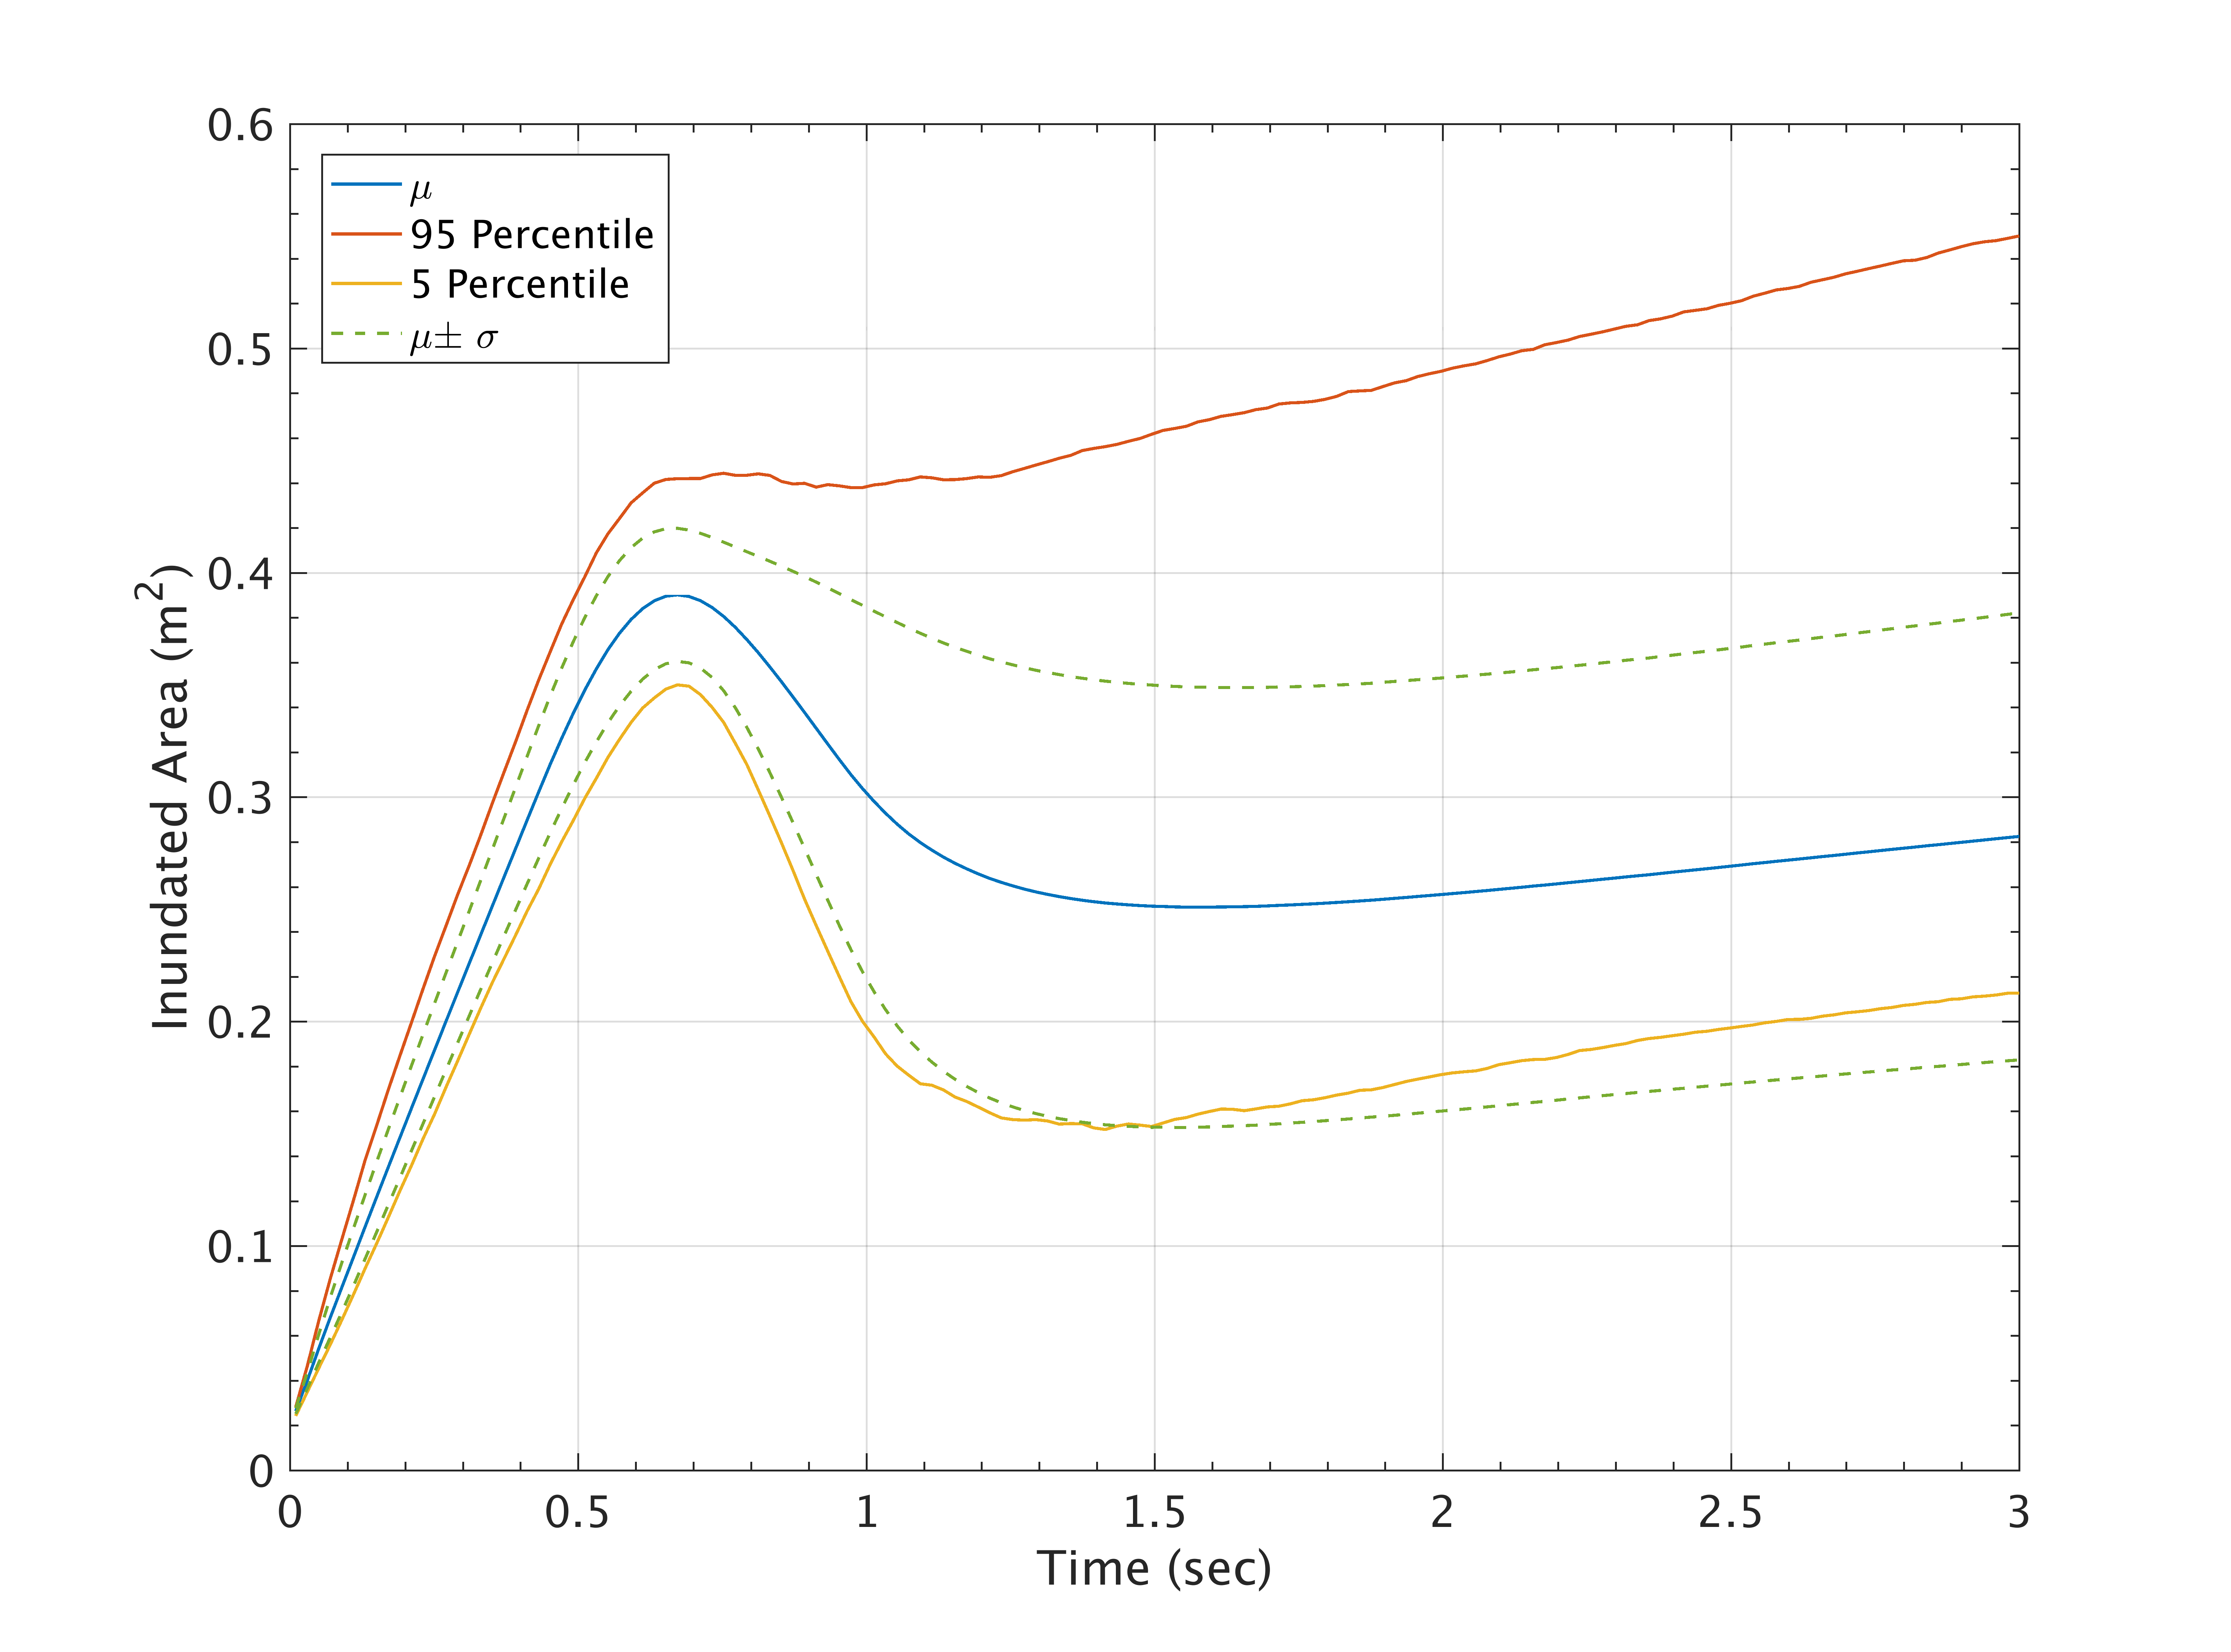
\includegraphics[width=1\textwidth]{InclinedPlane/GlobalRecords/C_Global_Ar.png}
                \subcaption{Mohr-Coulomb model.}
                \label{fig:Ramp-SP-InundAr-C}
        \end{minipage}
        \begin{minipage}[b]{0.5\linewidth}
                \centering
                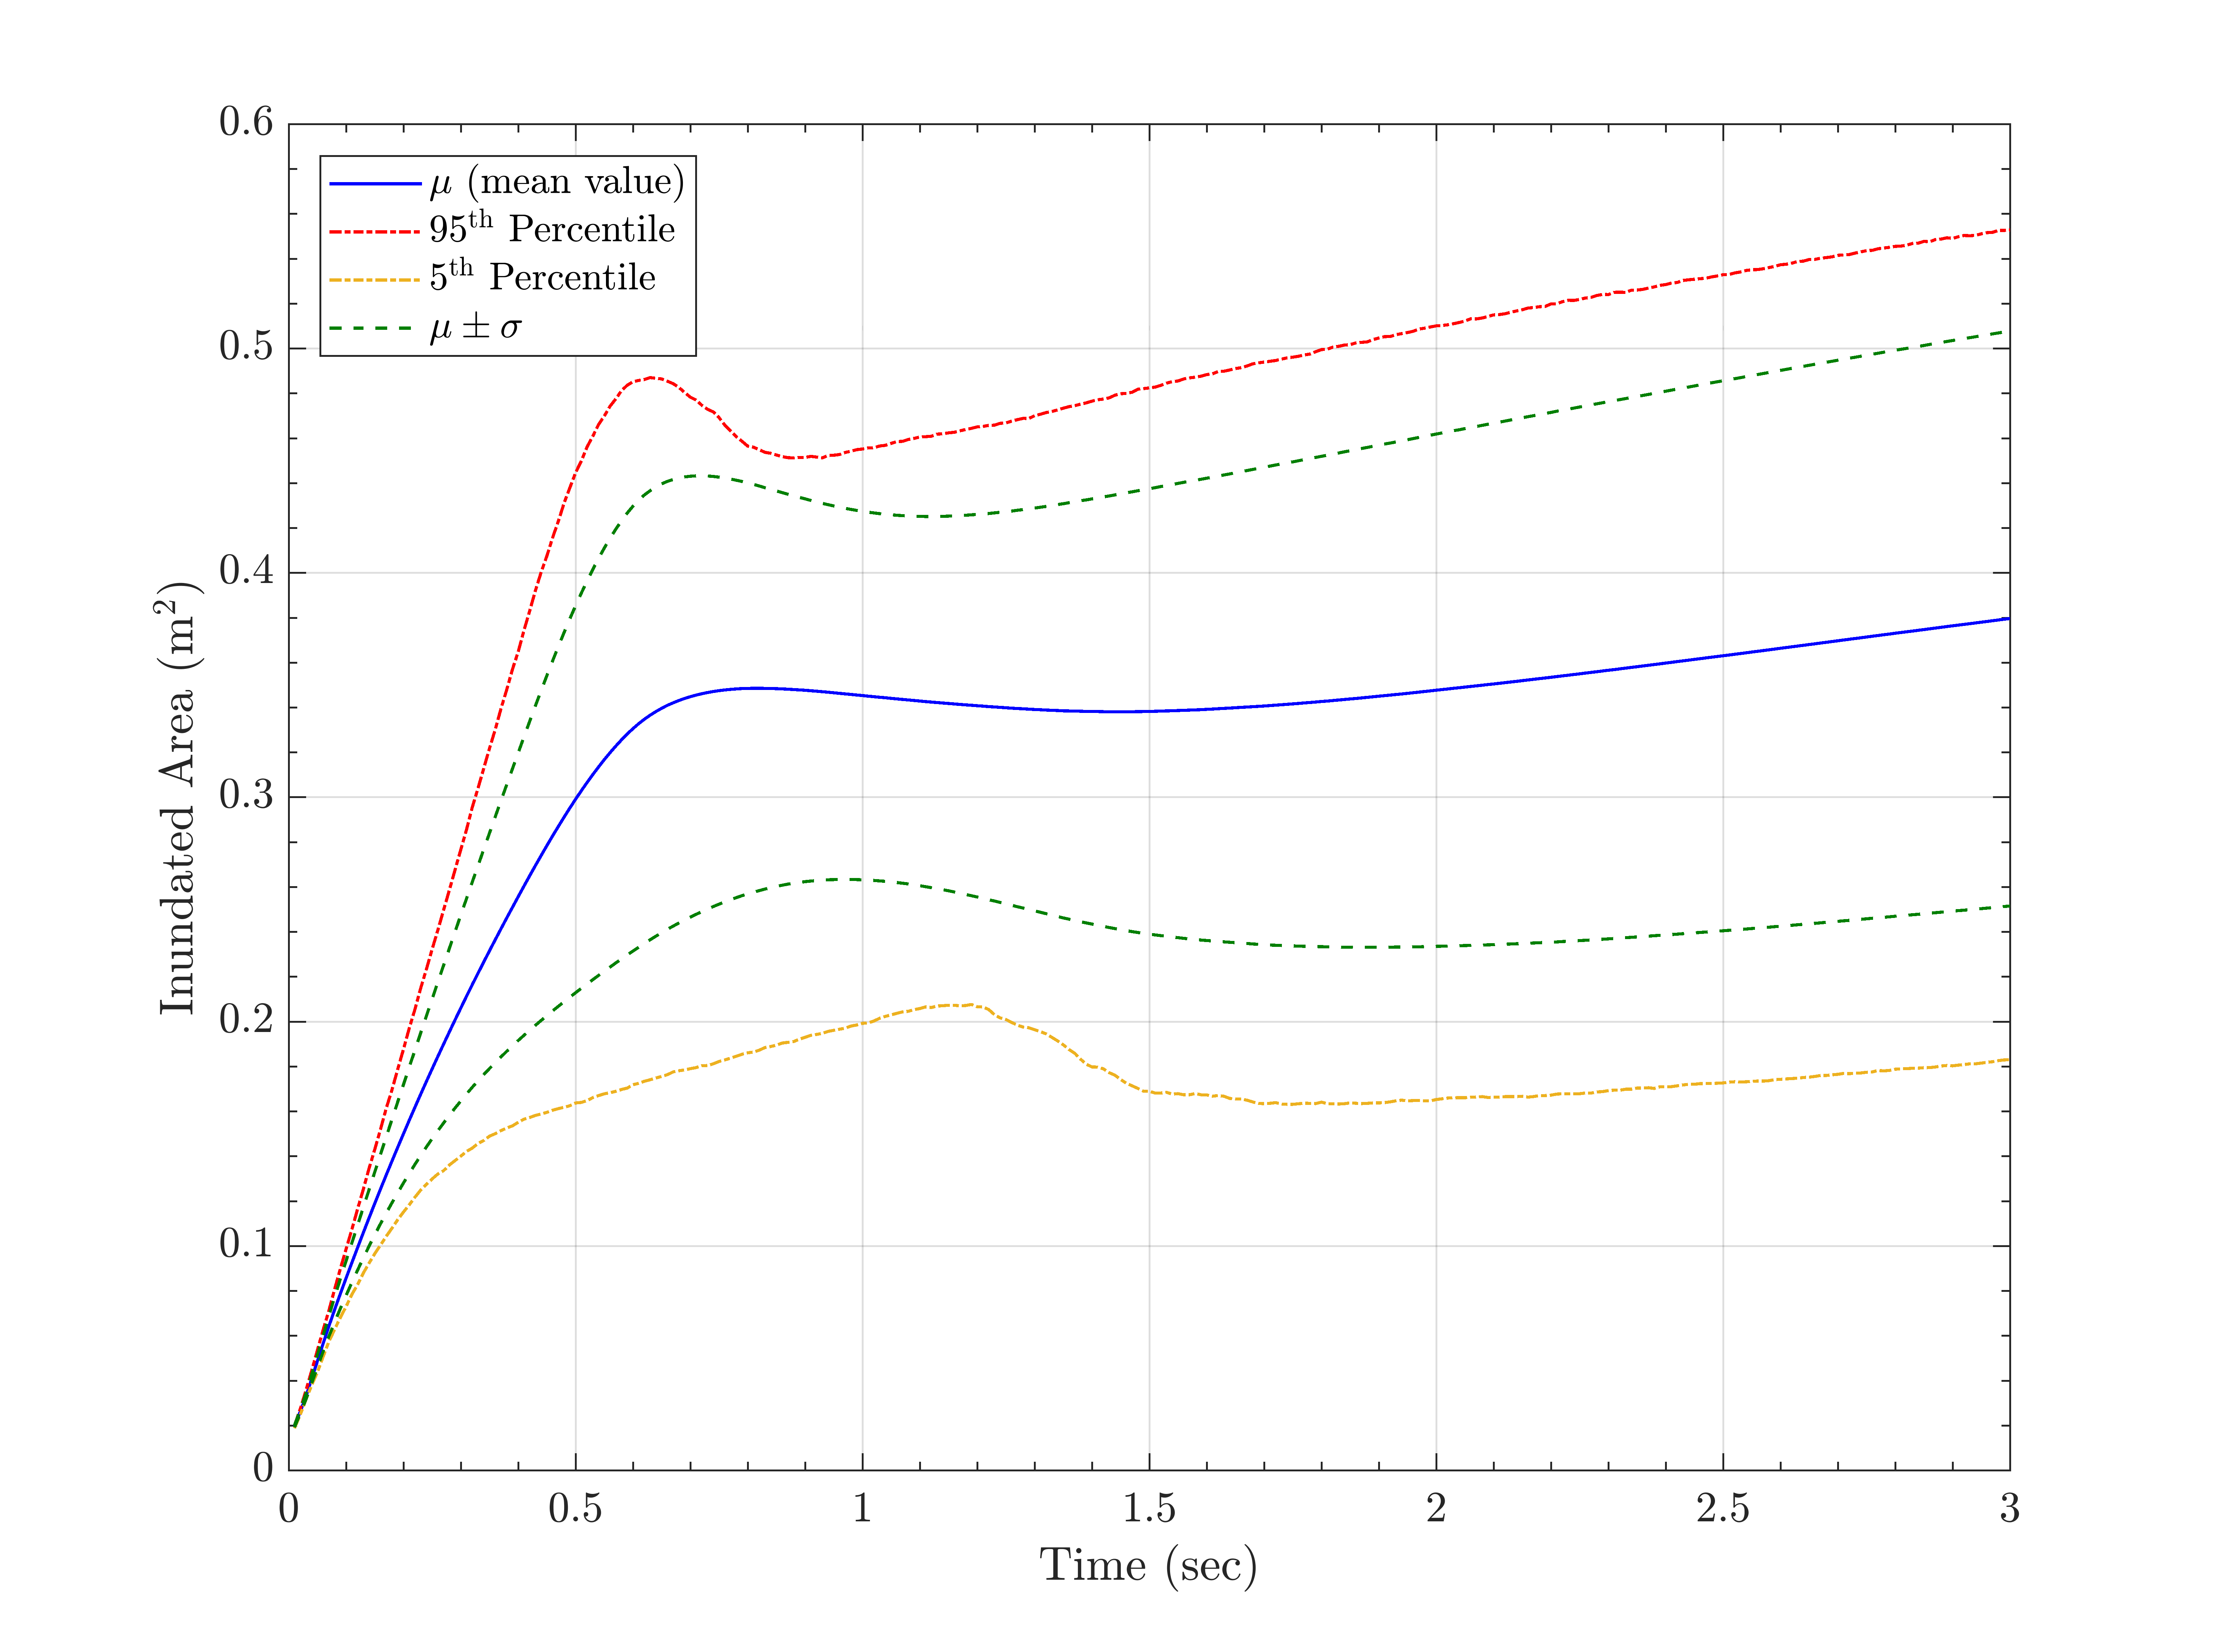
\includegraphics[width=1\textwidth]{InclinedPlane/GlobalRecords/P_Global_Ar.png}
                \subcaption{Pouliquen-Forterre model.}
                \label{fig:Ramp-SP-InundAr-P}
        \end{minipage}

        \begin{minipage}[b]{1\linewidth}
                \centering
                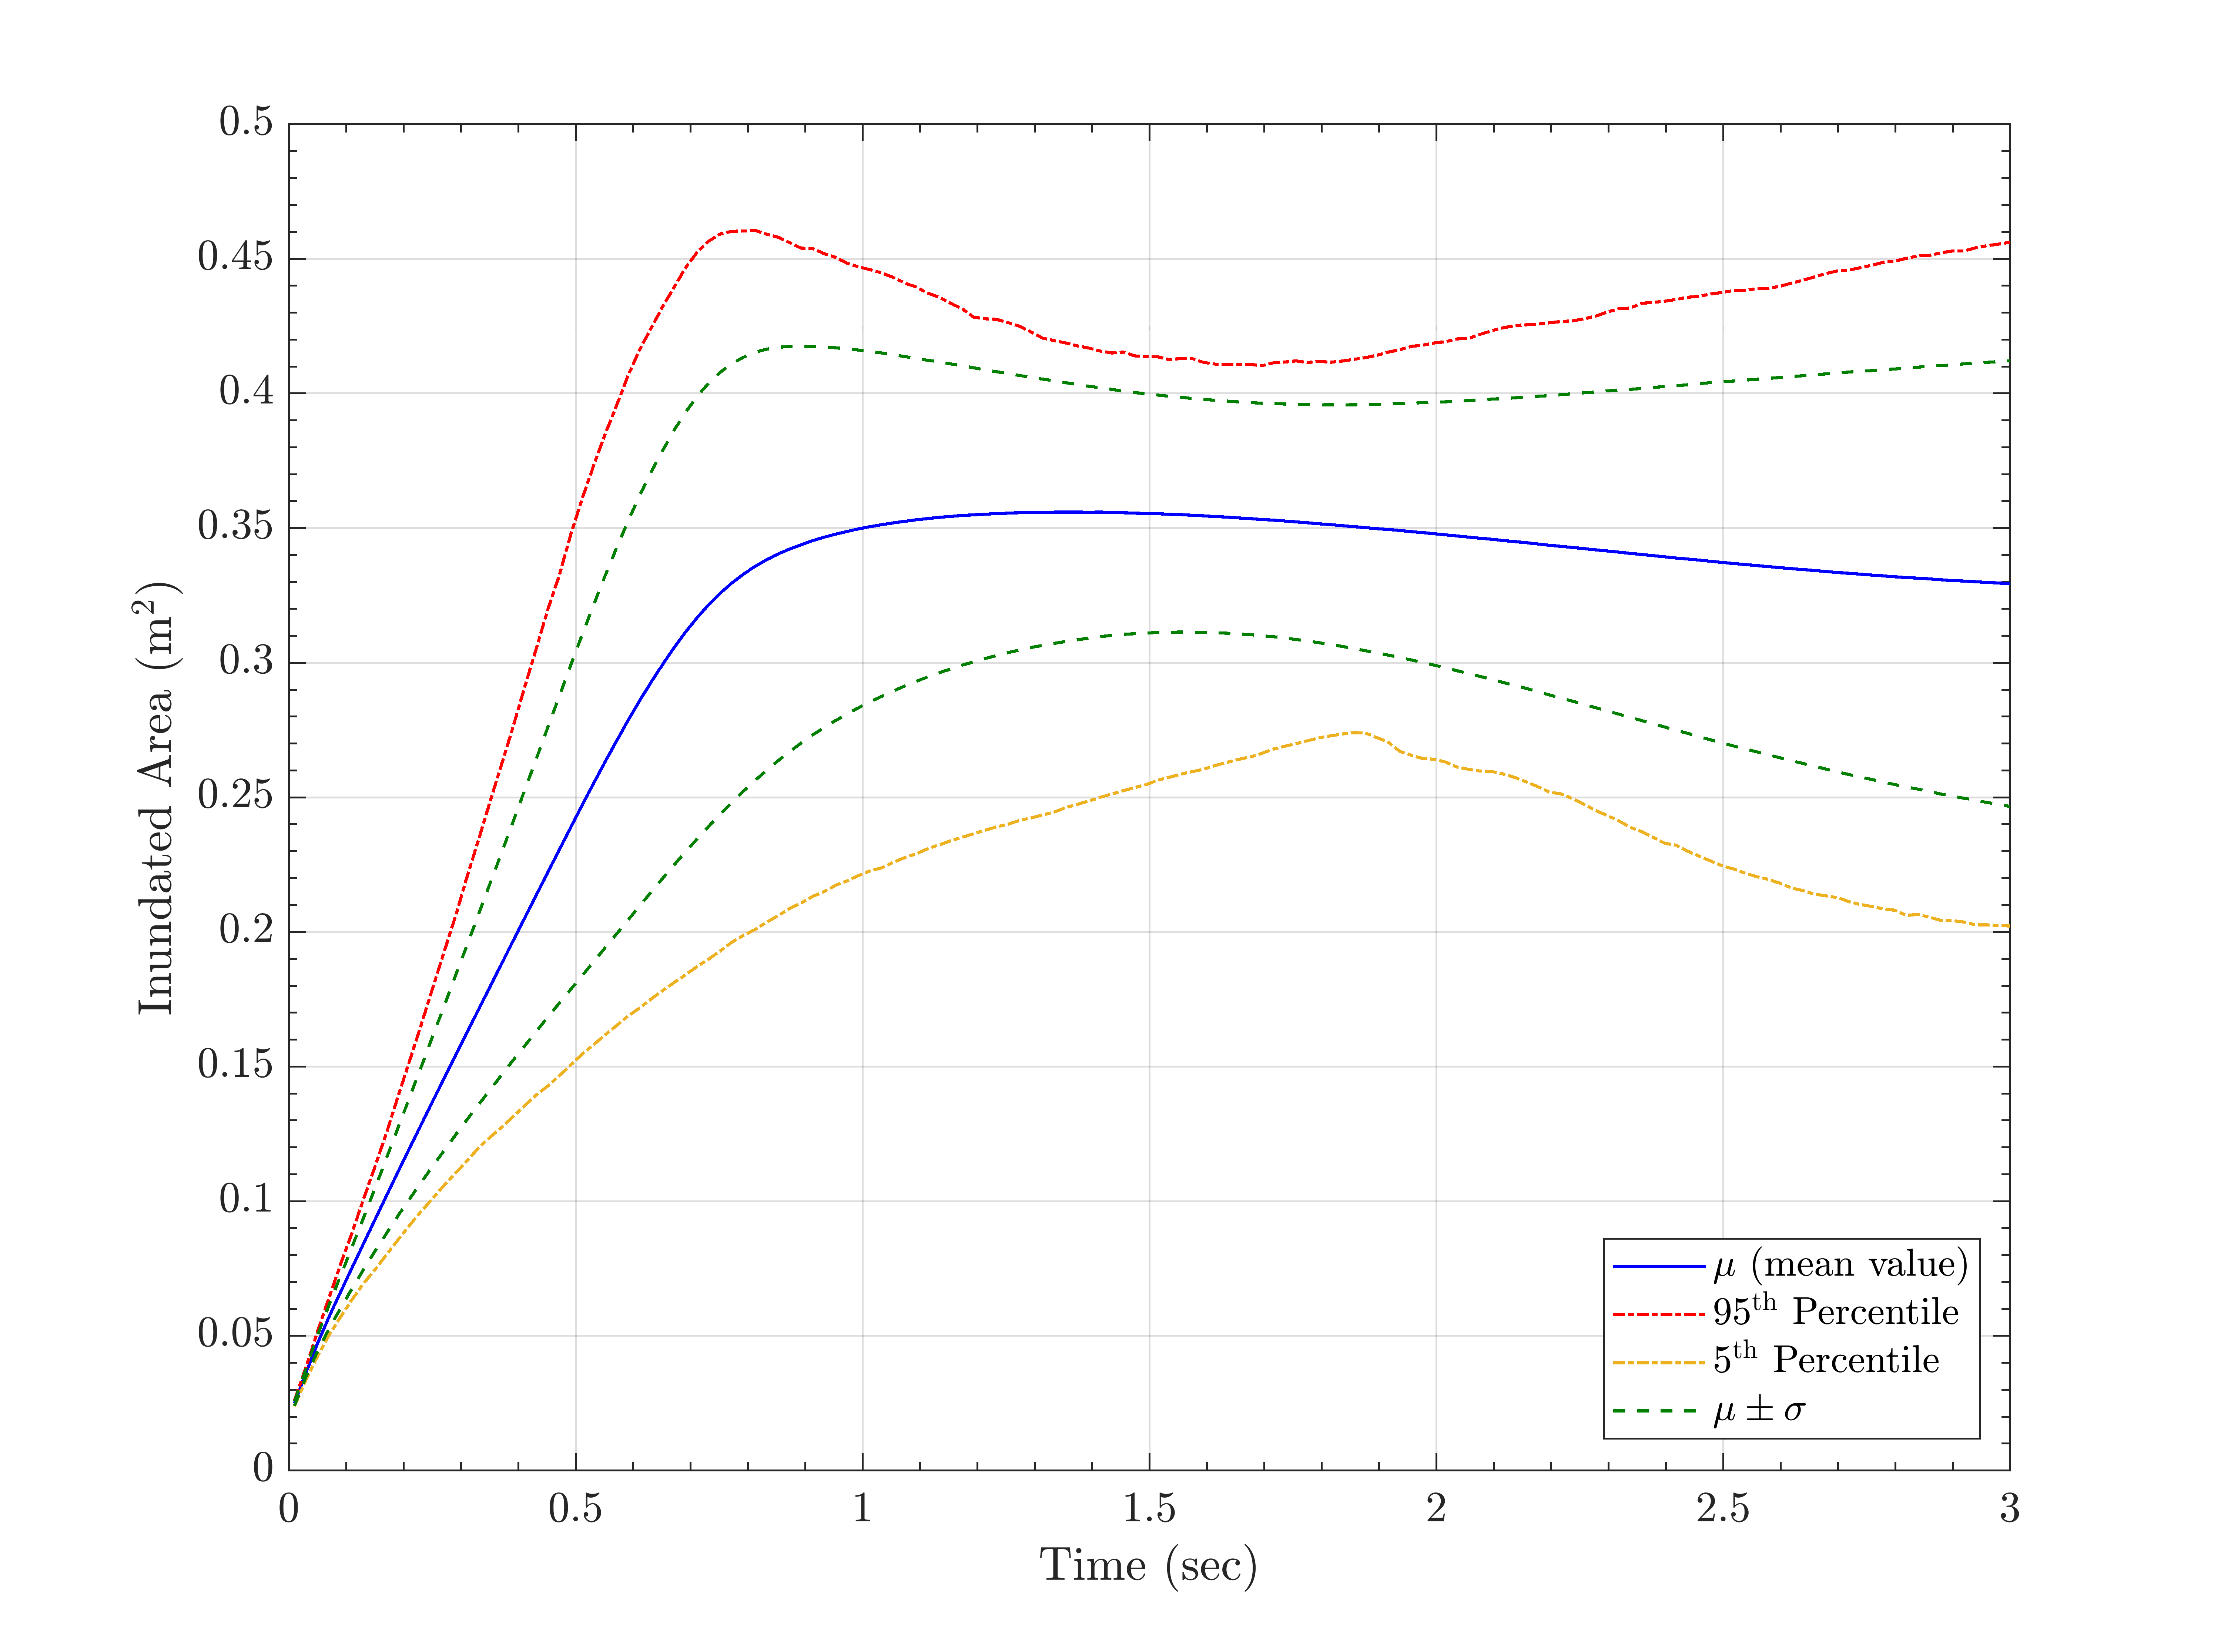
\includegraphics[width=0.5\textwidth]{InclinedPlane/GlobalRecords/V_Global_Ar.png}
                \subcaption{Voellmy-Salm model.}
                \label{fig:Ramp-SP-InundAr-V}
        \end{minipage}
        \caption{Full statistics of temporal records of inundated area by the flowing material.}
        \label{fig:Ramp-SP-InundAr}
\end{figure}

\section{Results and Discussion -- All}

\newpage
\bibliographystyle{unsrt}
\bibliography{mybibfile}

\end{document}
